\documentclass[11pt, twoside,a4paper]{book}
\usepackage{doc}
\usepackage{a4wide}
\usepackage{makeidx}
\usepackage[tight,footnotesize]{subfigure}
\usepackage{amsmath}
\usepackage{amsfonts}
\usepackage{multirow}
\usepackage{booktabs}
\newtheorem{theorem}{Theorem}
\newtheorem{problem}{Problem}
\newtheorem{definition}{Definition}
\usepackage{graphicx}
\graphicspath{{./figs/}}
%\usepackage{algorithmic}
\usepackage{listings}
\usepackage[utf8]{inputenc}
\usepackage[noend]{algpseudocode}
\usepackage{hyperref}
\hypersetup{
colorlinks,
citecolor=black,
filecolor=black,
linkcolor=black,
urlcolor=black
}
\usepackage[table]{xcolor}
\newcommand{\mat}[1]{\ensuremath{#1}}
\newcommand{\vek}[1]{{\ensuremath{\mathbf #1}}}
\newcommand{\figref}[1]{Figure~\protect\ref{#1}}
\newcommand{\secref}[1]{Section~\protect\ref{#1}}
\newcommand{\chapref}[1]{Chapter~\protect\ref{#1}}
\newcommand{\defref}[1]{Definition~\protect\ref{#1}}
\newcommand{\coderef}[1]{Algorithm~\protect\ref{#1}}
\newcommand{\appref}[1]{Appendix~\protect\ref{#1}}


\usepackage{color}
\definecolor{lightgray}{rgb}{.9,.9,.9}
\definecolor{darkgray}{rgb}{.4,.4,.4}
\definecolor{purple}{rgb}{0.65, 0.12, 0.82}

\lstdefinelanguage{JavaScript}{
keywords={typeof, new, true, false, catch, function, return, null, catch, switch, var, if, in, while, do, else, case, break,for},
keywordstyle=\color{blue}\bfseries,
ndkeywords={class, export, boolean, throw, implements, import},
ndkeywordstyle=\color{darkgray}\bfseries,
identifierstyle=\color{black},
sensitive=false,
comment=[l]{//},
morecomment=[s]{/*}{*/},
commentstyle=\color{purple}\ttfamily,
stringstyle=\color{red}\ttfamily,
morestring=[b]',
morestring=[b]"
}

\lstset{
language=JavaScript,
backgroundcolor=\color{lightgray},
extendedchars=true,
basicstyle=\footnotesize\ttfamily,
showstringspaces=false,
showspaces=false,
numbers=left,
numberstyle=\footnotesize,
numbersep=9pt,
tabsize=2,
breaklines=true,
showtabs=false,
captionpos=b
}
\renewcommand{\lstlistingname}{Algorithm}

\newcommand{\setR}{\ensuremath{\mathbb{R}}}
\newcommand{\col}{\ensuremath{c}}
\newcommand{\row}{\ensuremath{r}}
\newcommand{\field}[1]{\mathbb{#1}}
\newcommand{\R}{\ensuremath{\field{R}}}
\newcommand{\sparsifysymbol}{\ensuremath{\rho}}
\newcommand{\sparsify}[1]{\ensuremath{\sparsifysymbol(#1)}}
\newcommand{\todo}[1]{\textbf{#1}}
\newcommand{\nnz}[1]{\ensuremath{\operatorname{nz}(#1)}}
% Define the name of the two minimization problems
\newcommand{\MinStaBic}{\textsc{Minimum Star Bicoloring}}
\newcommand{\MinUniCom}{\textsc{Minimum Unidirectional Compression}}
\newcommand{\MinBidCom}{\textsc{Minimum Bidirectional Compression}}

\newcommand{\MinRStaBic}{\textsc{Minimum Restricted Star Bicoloring}}
\newcommand{\MinRUniCom}{\textsc{Minimum Restricted Unidirectional Compression}}
\newcommand{\MinRBidCom}{\textsc{Minimum Restricted Bidirectional Compression}}

\begin{document}
\pagenumbering{roman}
\begin{titlepage}
\centering

\includegraphics[width=0.3\linewidth]{logo}
\par
\vspace{2cm}
{\uppercase{\Large Combinatorial Scientific Computing\par}}
\vspace{2cm}
{\Large Mohammad Ali Rostami\par}
{\Large Supervisor: Prof. Martin B{\"u}cker\par}
\vspace{1cm}
{\Large Faculty of Mathematics and Computer Science\\Friedrich Schiller University Jena\par}
\vspace{2cm}
{\Large \today}
\end{titlepage}
\chapter*{Abstract}
Solving problems originating from the real-world applications are often based
on the solution to some linear equations containing a sparse Jacobian matrix.
These sparse Jacobian matrices are most of the time huge. Hence, there
is much research to exploit the sparsity structure and to decrease the amount of needed storage. In contrast to full Jacobian computation in which all elements are meant to be determined, partial Jacobian computation is looking at a subset of these elements. This property brings a lot of conventions leading to a faster
and more efficient computation.
Determining these nonzero elements in full or partial Jacobian computations by automatic differentiation techniques
can be modeled as graph coloring in graph language.

Since a matrix-vector product (instead of the whole Jacobian)
is needed in iterative solvers, automatic differentiation fits
the best in the iterative solvers.
On the other hand, the preconditioning techniques are used to improve the convergence of iterative solvers and need access to the nonzero elements. So, a sparsification applies on the Jacobian before computing the preconditioner. The elements produced from the sparsification are also considered as the required elements in the partial coloring.
There is a procedure which selects a subset of the remaining nonrequired elements and adds to the sparsified matrix such that no fill-ins or increase of the number of colors happens.
The current thesis first looks at different ways to optimize
the processes of selecting elements.
At the second part of this thesis, we introduce an interactive educational module to teach these
tricky concepts in the classroom.

\chapter*{Zusammenfassung}
\chapter*{Acknowledgements}
\noindent This project would not have been possible without
the support of many people. I must express my first gratitude
towards \textit{Prof. Dr. Martin B\"ucker} for his continuous
support during my research, patience, immense knowledge,
and attention to details.
I should confess that I can not imagine a better and friendlier supervisor.
Besides, I would like to thank \textit{Michael Lülfesmann}
Finally, I wish to thank my wife \textit{Masoumeh Seydi} and
my best friend \textit{Azin Azadi} for encouraging me throughout all my studies at University.

\tableofcontents
\chapter{Introduction}
\pagenumbering{arabic}
Partial differential equations (PDE) are the most common models of the real-world problems. Iterative solvers are a solution to these linear systems which need a multiplication of Jacobian and a vector in each iteration.
Many strategies were studied to compute these products efficiently.
Automatic Differentiation~\cite{Griewank2008EDP,Rall1981ADT} computes not only the differentiation without numerical errors but also the matrix-vector multiplication automatically.
Based on this ability of AD techniques, different methods are analyzed to reduce the memory that is needed to store the Jacobian matrix as well as speeding up the computation. These methods are parts of a bigger area called combinatorial scientific computing.

On the other hand, another method to speed up the convergence of the linear solver
is preconditioning. The preconditioning techniques need most of the time access to
the elements of Jacobian which is in contrast to the requirements of automatic differentiation.
Applying a sparsification operator first on the Jacobian matrix and do the ILU preconditioning
on the sparsified matrix would be a solution to the problem of determination of
all elements. This process becomes complete by trying to add more elements to the matrix
without producing more fill-ins or colors. We introduce new heuristics to for this purpose.

This dissertation is structured as follows.
First, we go through basic definitions in \chapref{prel} needed in other chapters.
We discuss the known graph models for full Jacobian computation and partial Jacobian
computation. A sparsification is introduced which helps in the formulation of
mix of automatic differentiation and preconditioning.
\chapref{package} discusses new heuristics for distance-$2$ coloring and
star bicoloring. We also look at a simple parallelization technique for the
coloring algorithm. Also, we look at the ordering for the ILU preconditioning.
In this chapter, we restructure a previous software
to be more readable and extensible and to contain new heuristic algorithm.
\chapref{explain} discuss an interactive educational module
which is designed to teach the computational science algorithms in the classroom.
Finally, the conclusion and future work come in \chapref{conc}.

\chapter{Graph Models from Scientific Computing}
\label{prel}
In this chapter, we would briefly discuss already existing concepts which we need to understand
the other parts of the paper. In each section of this chapter,
we provide some references to read these concepts further in details.
We look at the ideas to determine the nonzeros of sparse matrices in
\secref{s.det.nonzero}. Then, the block diagonal sparsification
and its corresponding combinatorial model is discussed~\secref{s.block.diag.sp}.
Finally, we look at definitions on mixing ILU preconditioning and AD, and
a corresponding bipartite graph model in \secref{s.precond}.

%===================================================================================================
\section{Determining Nonzeros of Sparse Matrices}
\label{s.det.nonzero}
%===================================================================================================
There are many literature on exploiting the sparsity pattern of the Jacobian matrix
to improve the automatic differentiation and its several applications.
Here, we look at the two parts of full and partial Jacobian computation in
\secref{s.full.jac} and \secref{s.part.jac}.
%===================================================================================================
\subsection{Full Jacobian Computation}
\label{s.full.jac}
%===================================================================================================
If there is a program which computes the function $f(x) : \setR^n \rightarrow \setR^m$
in the computational cost $t$,
techniques of automatic differentiation (AD)~\cite{Griewank2008EDP,Rall1981ADT} generate
Computer programs capable of evaluating the $m \times n$ Jacobian matrix $J$.
The so-called forward mode of automatic differentiation creates a program automatically
which computes the product of Jacobian matrix with some given so-called seed matrix $V$,
i.e. $JV$. There is an inverse mode of automatic differentiation which computes the product $WJ$.
These techniques of automatic computes the Jacobian $J$ without assembling it.

Suppose the matrix $V$ has $\col$ number of columns and the matrix $W$ has $\row$ number of rows,
the computational costs to compute these products would be $\col t$ and $\row t$, respectively.
In general, the Jacobian $J$ is computed choosing either $c=n$ and $V$ as the identity of
order~$n$ in the forward mode or $r = m$ and $W$ as the identity of order $m$ in the
reverse mode. However, if $J$ is sparse and its sparsity pattern is known the number of
columns of~$V$ in the forward mode or the number of rows of~$W$ in the reverse mode can
be reduced to $\col < n$ or $\row < m$ such that all nonzero entries of $J$ still appear
in the product $JV$ or $WJ$. This way, the computational cost is decreased using either
the forward mode with a suitable linear combination of the columns of~$J$ or the reverse
mode with a suitable linear combination of the rows of~$J$; see the
survey~\cite{Gebremedhin05whatcolor}.
In \secref{ss.problem.full} and \secref{ss.problem.full}, we formulate problems to compute the
minimum values for $\col$ and $\row$ and the corresponding combinatorial problem.
%===================================================================================================
\subsubsection{Problem}
\label{ss.problem.full}
%===================================================================================================
Here, we formulate a problem to find the optimal seed matrix in which
the number of rows and columns are smaller than the actual Jacobian matrix, so called compression.
A unidirectional compression is a compression in either rows or columns in contrast to
a bidirectional compression in which both rows and columns are compressed in the same time.
The key idea behind this \emph{unidirectional compression} is now illustrated for the
forward mode. First, we present a definition as follows,
\begin{definition}[Structurally Orthogonality]
\label{d:struct_orth}
Let $J=[c_1, c_2, \dots, c_n]$ denote the Jacobian matrix in which $c_i \in \setR^m$ is the $i$th
column. Two columns $c_i$ and $c_j$ are
called \emph{structurally orthogonal} if they do not have any nonzero element in a same
row. Two columns are called \emph{structurally non-orthogonal} if there is at least one
row in which both columns, $c_i$ and $c_j$, have a nonzero element.
Analogously, two rows are
\emph{structurally orthogonal} if they do not have any nonzero element in the same column.
\end{definition}
We can compute a linear combination of structurally orthogonal columns of the seed matrix
to reduce the number of columns of the seed matrix. This linear combination contains actually all elements of each columns. The definition of the structurally orthogonal columns can be similarly adapted to rows. The number of structurally orthogonal groups scales with the computational cost either for columns or rows.
\figref{f.mat-ex-for-orth} (Left) and \figref{f.mat-ex-for-orth} (Middle) shows two examples
of the matrices which can be compressed efficiently by columns and rows, respectively.
\begin{figure}
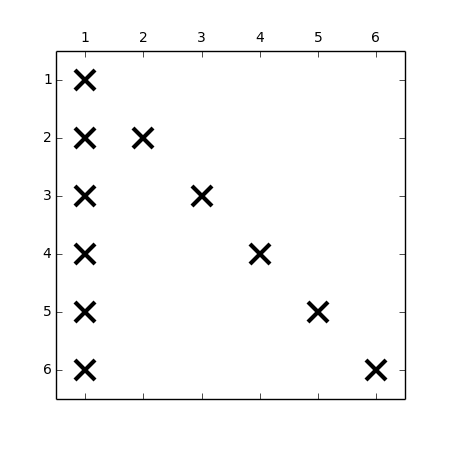
\includegraphics[width=0.3\linewidth]{diag-col}
\hfill
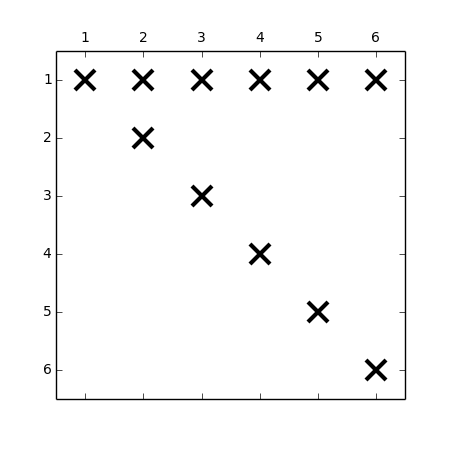
\includegraphics[width=0.3\linewidth]{diagrow}
\hfill
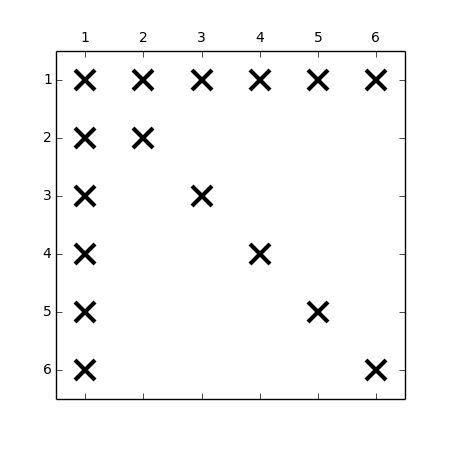
\includegraphics[width=0.3\linewidth]{arrow}
\caption{
(Left) An example of a matrix compressed efficiently by columns.
(Middle) An example of a matrix compressed efficiently by rows.
(Right) An example of a matrix which cannot be compressed efficiently either by columns nor by rows.
}
\label{f.mat-ex-for-orth}
\end{figure}
Now, consider the matrix $C$ in \figref{f.mat-ex-for-orth} (Right) that has neither structurally orthogonal columns nor structurally orthogonal rows.
Therefore, there is no unidirectional compression of the
matrix $C$, neither by \col\ columns nor by \row\ rows which reduce \col\ or \row\ below
the number of columns or rows.
The technique of bidirectional, which compresses both columns and rows in the same time, will reduce the computational cost. This technique computes both forward and reverse mode of automatic differentiation.

For general sparsity patterns,
it is not straightforward to figure out how to linearly combine columns and rows such that
the computational cost is minimized. Hence, we introduce the combinatorial
optimization problems~\ref{p.seed.uni} and ~\ref{p.seed.bid}
for unidirectional or bidirectional compressions to determine the nonzero elements of huge Jacobians efficiently.

\begin{problem}[\MinUniCom]
\label{p.seed.uni} Let $J$ be a sparse ${m\times n}$ Jacobian matrix with known sparsity
pattern. Find a seed matrix $V$ of dimension $n\times \col$
whose number of columns of $V$ sums up
to a minimal value, $\col$, such that all nonzero elements of $J$ also appear in
the matrix-matrix product $JV$.
\end{problem}

\begin{problem}[\MinBidCom]
\label{p.seed.bid} Let $J$ be a sparse ${m\times n}$ Jacobian matrix with known sparsity
pattern. Find a pair of binary seed matrices $V$ of dimension $n\times \col$ and $W$~of
dimension $\row \times m$ whose number of columns of $V$ and number of rows of $W$ sum up to a minimal value, $\col + \row$, such that all nonzero elements of $J$ also appear in
the matrix-matrix products $JV$ and $WJ$.
\end{problem}

%==========================================================================================
\subsubsection{Combinatorial Model}
\label{s.modeling.full}
%==========================================================================================
We reformulate the scientific computing problems which
we have discussed in \secref{ss.problem.full}.
The new formulation is an equivanet problem defined on a
carefully chosen graph model. The survey \cite{Gebremedhin05whatcolor}
discusses different methods
to exploit the sparsity involved in derivative computations.
We first look at a simple graph model for the unidirectional compression,
%
\begin{definition}[Column Intersection Graph]
\label{d:cig}
The column intersection graph $G = (V,E)$ associated with an $n \times n$ Jacobian $J$
consists of a set of vertices $V=\{v_1, v_2, \dots, v_n\}$ whose vertex $v_i$ represents
the $i$th column $J(:,i)$. Furthermore, there is an edge $(v_i,v_j)$ in the set of edges
$E$ if and only if the columns $J(:,i)$ and $J(:,j)$ represented by $v_i$ and $v_j$ have
a nonzero element in at least a same row position.
\end{definition}

As we have a graph model intrepreted from our Jacobian matrix in \defref{d:cig},
the grouping of columns can be encoded in the following well-know graph coloring problem.
%
\begin{definition}[Coloring]
A coloring of $G$ is a mapping $\Phi : V \to {1, \dots, p}$ with the property
$\Phi(v_i)\neq \Phi(v_j)$ for $(v_i,v_j) \in E$.
\end{definition}
%
Coleman and Mor\'{e} \cite{Coleman1983EoS} then showed that Problem~\ref{p.seed.uni}, which
asks for a seed matrix with a minimal number of columns, is equivalent to the following
coloring problem.

\begin{problem}[Minimum Coloring]
\label{p:mincol}
Find a coloring $\Phi$ of the column intersection graph $G$ with a minimal number of
colors.
\end{problem}

As shown, there is an intimate connection between the sparse Jacobian computations described in Problem~\ref{p.seed.uni} and the graph coloring issues described by Problem~\ref{p:mincol}.
If a vertex represents a row and an edge represents structural
non-orthogonality of two rows a row-intersection graph can be adapted too.

Although, this model is convincing for the unidirectional compression,
the bidirectional compression can not be an instance of model.
A bidirectional compression needs the information of both rows and columns. Therefore, a bipartite graph model is defined for this purpose as in~\cite{Coleman1996SaE,cv:ecs,hs:csj}.

\begin{definition}[Bipartite Graph Model]
\label{d.bip.graph}
In the bipartite graph model, the vertex set $V=V_c\cup V_r$
is decomposed into a set of vertices~$V_c$ representing columns of $J$ and another set of
vertices~$V_r$ representing rows. The set of edges~$E$ is used to represent the nonzero
elements and it is defined as follows. An edge $(c_i , r_j) \in E$ connects a column
vertex $c_i \in V_c$ and a row vertex $r_j \in V_r$ if there is a nonzero element in $J$
at the position represented by $c_i$ and $r_j$. The graph is bipartite indicating that
all edges connect vertices from one set~$V_c$ to the other set $V_r$. That is, there is
no edge connecting vertices within the set $V_c$ or within $V_r$. Moreover, two vertices
that are connected by a path of length two, are called \emph{distance-$2$ neighbors}.
\end{definition}

The coloring problem in the column-intersection graph \ref{p.seed.uni} can also be represented in
this bipartite graph model. This equivalent coloring is done only in the set of
column vertices. Also, \emph{distance-$2$ neighbors} should be considered instead of
the classic definition of neighborhood.

The overall idea behind transforming Problem \ref{p.seed.bid}, \MinBidCom, into an equivalent
problem using the bipartite graph model is as follows. The grouping of the columns and
rows is expressed by representing each group by a color. Vertices that belong to the same
group of columns/rows are assigned the same color. Formally, this is represented by a
coloring of a bipartite graph. Such a coloring is mapping
$$
\Phi:V_c \cup V_r \to \{0,1,\dots ,p\}
$$
that assigns to each vertex a color represented by an integer. Recall from the previous
section that, in general, there can be columns or rows that are not chosen in the
grouping at all. Therefore, the coloring~$\Phi$ also involves a ``neutral'' color
representing this ``don't color'' situation. A vertex $v \in V_c \cup V_r$ that is not
used in the grouping of columns/rows is assigned the neutral color $\Phi(v)=0$. More
precisely, if $\Phi(v)=0$ for a column vertex $v$ then every nonzero represented by an
incident edge of $v$ is determined by a linear combination of rows. Similarly, a nonzero
entry represented by an edge that is incident to a neutrally-colored row vertex is
determined by a linear combination of columns.

To represent the process of finding seed matrices using the bipartite graph model, it is
necessary to consider the underlying properties, which are as follows:
\begin{enumerate}
\item The computational cost roughly consists of the number of groups of columns and
rows. Since the overall cost is the sum of the costs associated to the forward mode
and to the reverse mode, the (non-neutral) colors for the forward mode and the
(non-neutral) colors for the reverse mode need to be different.

\item Recall from our example with the products $CV$ and $WC$ that some nonzero
elements may be computed twice, by the forward mode in $JV$ and by the reverse mode
in $WJ$. Therefore, an edge representing such a nonzero element connects two
vertices with two different non-neutral colors. In general, since problem
\MinBidCom\ asks for computing \emph{all} nonzero elements, at least one vertex of
every edge has to be colored with a non-neutral color.

\item Recall from the example that structural orthogonality is no longer required for
grouping the rows and columns. However, there is still the following restriction.
Suppose two columns are structurally non-orthogonal and have a nonzero element in a
same row. If this row is not handled by the reverse mode, these two columns need to
be in different column groups. The same argument holds for corresponding situations
with row groups.

\item Consider three nonzero elements in matrix positions $(i,k)$, $(i,\ell)$, and
$(j,k)$. Suppose that the nonzero at $(i,k)$ is computed by the reverse mode
assigning some (non-neutral) color to the row vertex $r_i$. Then, if $(j,k)$ is
also computed via the reverse mode, a second (non-neutral) color is needed for
$r_j$. Now, if $(i,\ell)$ is already determined by the reverse mode for row $i$ the
column vertex $c_\ell$ is assigned the neutral color. However, if $(i,\ell)$ is
computed by the forward mode, a third (non-neutral) color is needed for $c_\ell$. A
similar argument holds if $(i,k)$ is computed by the forward mode.

\end{enumerate}

Based on these considerations, the following definition captures these properties.

\begin{definition}[Star Bicoloring]\label{d.coloring}
Given a bipartite graph $G=(V_c\cup V_r, E)$, then a mapping $\Phi:V_c \cup V_r \to
\{0,1,\dots ,p\}$ is a star bicoloring of $G$ if the following conditions are satisfied:
\begin{enumerate}
\item Vertices in $V_c$ and $V_r$ receive disjoint colors, except for the neutral color~$0$. That
is, for every $c_i \in V_c$ and $r_j \in V_r$, either $\Phi(c_i) \neq \Phi(r_j)$ or
$\Phi(c_i)=\Phi(r_j)=0$.

\item At least one vertex of every edge receives a non-neutral color. That is, for every
$(c_i,r_j)\in E$, the conditions $\Phi(c_i)\neq 0$ or $\Phi(r_j)\neq 0$ hold.

\item For every path $(u,v,w)$ with $\Phi(v) = 0$, the condition $\Phi(u)\neq \Phi(w)$ is
satisfied.
\item Every path of length three with four vertices uses at least three colors
(possibly including the neutral color).
\end{enumerate}
\end{definition}

Using the bipartite graph model and the definition of a star bicoloring, the problem
\MinBidCom\ is equivalent to the following graph problem.

\begin{problem}[\MinStaBic]
\label{p.coloring} Given the bipartite graph $G=(V_r\cup V_c, E)$ associated to a sparse Jacobian
matrix~$J$, find a star bicoloring of $G$ with a minimal number of non-neutral colors.
\end{problem}

A unidirectional compression is a special case of a bidirectional compression. More precisely, a
unidirectional compression with respect to columns corresponds to a star bicoloring in which all
the vertices in $V_c$ are colored with a non-neutral color and all row vertices are colored with
the neutral color. This way, the coloring constraint of a star bicoloring reduces to coloring
distance-$2$ neighbors in the bipartite graph using different (non-neutral) colors. This distance-2
coloring in the bipartite graph model is then equivalent to a coloring in the undirected graph
model in which all neighbors are colored differently. Finally, a discussion of the computational
complexity of Problem~\ref{p.coloring} including recent new results is given in~\cite{jj:cjr}.

%To illustrate the tricky transformation from \MinBidCom\ to \MinStaBic, we design a new
%educational module explained in Section~\ref{s.bidirectional}.
%%%%%%%%%%%%%%%%%%%%%%%%%%%%%%%%%%%%%%%%%%%%%%%%%%%%%%%%%%%%%%%%%%%%%%%%%%%%%%%%%%%%%%%%%%%%%%%%%%%%%%%%%
\subsection{Partial Jacobian Computation}
\label{s.part.jac}
%%%%%%%%%%%%%%%%%%%%%%%%%%%%%%%%%%%%%%%%%%%%%%%%%%%%%%%%%%%%%%%%%%%%%%%%%%%%%%%%%%%%%%%%%%%%%%%%%%%%%%%%%
Gebremedhin et al~\cite{Gebremedhin05whatcolor} introduced the concept of the partial Jacobian computation
in which the assumption is that only a subset of Jacobian, so called the required elements,
should be determined.
L{\"u}lfesmann~\cite{Lulfesmann2012Fap} has studied more considerably in this area and
introduced some heuristics for partial computation.
%%%%%%%%%%%%%%%%%%%%%%%%%%%%%%%%%%%%%%%%%%%%%%%%%%%%%%%%%%%%%%%%%%%%%%%%%%%%%%%%%%%%%%%%%%%%%%%%%%%%%%%%%
\subsubsection{Problem}
\label{ss.problem.part}
%%%%%%%%%%%%%%%%%%%%%%%%%%%%%%%%%%%%%%%%%%%%%%%%%%%%%%%%%%%%%%%%%%%%%%%%%%%%%%%%%%%%%%%%%%%%%%%%%%%%%%%%%
Suppose the required elements are shown by $R$, the definition of
\emph{structurally orthogonality} is adapted for the partial coloring as follows,a
\begin{definition}[Partially Structurally Orthogonal]\label{d.part.str.orth}
Two columns $c_i$ and $c_j$ are partially structurally orthogonal with respect to $R$
if and only if they do not have a nonzero element in the same row where at least
one of these nonzero elements is required.
\end{definition}

The corresponding problem can be formulated as follows for either unidirectional
or bidirectional compression,
\begin{problem}[\MinRUniCom]
\label{p.seed.runi} Let $J$ be a sparse ${m\times n}$ Jacobian matrix with known sparsity
pattern and $R$ be a proper subset of $J$. Find a seed matrix $V$ of dimension $n\times \col$
whose number of columns of $V$ sums up
to a minimal value, $\col$, such that all nonzero elements of $R$ also appear in
the matrix-matrix product $JV$.
\end{problem}

\begin{problem}[\MinRBidCom]
\label{p.seed.rbid} Let $J$ be a sparse ${m\times n}$ Jacobian matrix with known sparsity
pattern and $R$ be a proper subset of $J$.
Find a pair of binary seed matrices $V$ of dimension $n\times \col$ and $W$~of
dimension $\row \times m$ whose number of columns of $V$ and number of rows of $W$ sum up
to a minimal value, $\col + \row$, such that all nonzero elements of $R$ also appear in
the pair of matrix-matrix products $JV$ and $WJ$.
\end{problem}

An equivalent graph-theoretical formulation of this problem is discussed in the next
section.

\subsubsection{Combinatorial Model}
Based on \cite{Gebremedhin05whatcolor,Lulfesmann2012Fap}, the definitions
of the full Jacobian colorings are adapted as follows,
\begin{definition}[Restricted distance-$2$ coloring]\label{d.coloring.d2}
Given a bipartite graph $G=(V_c\cup V_r, E)$ and a subset of required edges
$E_R\subset E$ , then a mapping $\Phi:V_c \to
\{0,1,\dots ,p\}$ is a distance-$2$ coloring
of $G$ restricted to $E_R$ if no column vertex gets a zero color and
for every path $(c_k,r_i,c_j)$ with $c_k\in V_c$,
$\Phi(c_k) \neq \Phi(c_j)$.
\end{definition}
\begin{definition}[Restricted star bicoloring]\label{d.coloring.bicol}
Given a bipartite graph $G=(V_c\cup V_r, E)$ and a subset of required edges
$E_R\subset E$ , then a mapping $\Phi:V_c \cup V_r \to
\{0,1,\dots ,p\}$ is a star bicoloring of $G$ restricted to $E_R$
if the following conditions are satisfied:
\begin{enumerate}
\item Vertices in $V_c$ and $V_r$ receive disjoint colors, except for the neutral color~$0$. That
is, for every $c_i \in V_c$ and $r_j \in V_r$, either $\Phi(c_i) \neq \Phi(r_j)$ or
$\Phi(c_i)=\Phi(r_j)=0$.

\item At least one end point of and edge in $E_R$ receives a nonzero color.
\item For every edge $(r_i,c_j)\in E_R$, $r_i, r_l\in V_r$, and
$c_j, c_k\in V_c$,
\begin{itemize}
\item if $\Phi (r_i) = 0$, then for every path $(c_k,r_i,c_j)$, $\Phi (c_k)\neq \Phi (c_j)$
\item if $\Phi (c_j) = 0$, then for every path $(r_i,c_j,r_l)$, $\Phi (r_i)\neq \Phi (r_l)$
\item if $\Phi (r_i) = 0$ and $\Phi (c_j) = 0$, then for every path $(c_k,r_i,c_j,r_l)$,
$\Phi (c_k)\neq \Phi (c_j)$ or $\Phi (r_i)\neq \Phi (r_l)$
\end{itemize}
\end{enumerate}
\end{definition}

The optimization problems would be to
find the minimum restricted distance-$2$ coloring
and the minimum restricted star bicoloring.
\section{Block Diagonal Sparsification}
\label{s.block.diag.sp}
Here, we look at the sparsification of the coefficient matrix $J$. The
sparsification of $J$ is represented by the symbol \sparsify{J}. The idea is to select a
subset of all nonzero elements of $J$, described by~\sparsify{J}, and construct a
preconditioner based on these selected nonzero elements~\cite{Cullum2006}. These nonzero
elements selected by \sparsify{J} are called \emph{required} nonzero elements. Throughout
this paper we consider the special case of a sparsification in the form of $k\times k$
blocks on the main diagonal. That is, the pattern of the required nonzero elements is
given by the pattern of all nonzero entries within these $k\times k$ blocks on the
diagonal. If the block size $k$ does not divide the matrix order $n$, we adapt the size
of the last diagonal block to some smaller value such that the sum of all block sizes
equals $n$. We formulate the new problem that represents the assembly of the
semi-matrix-free approach with a relative minimal cost as follows.
%
\begin{problem}[Block Seed]
\label{p:block}
%
Let $J$ be a sparse $n \times n$ Jacobian matrix with known sparsity pattern and let
\sparsify{J} denote its sparsification using $k \times k$ blocks on the diagonal of $J$.
Find a binary $n \times p$ seed matrix~$S$ with a minimal number of columns, $p$, such
that all nonzero entries of \sparsify{J} also appear in the compressed matrix $J \cdot
S$.
\end{problem}

We now focus on reformulating this combinatorial problem from
scientific computing regarding an equivalent problem defined on a suitable graph model.
Recall that the set of nonzero elements is divided into required and nonrequired
elements. Two columns can be linearly combined without losing information on the
required elements as long as one of the following conditions is satisfied:
\begin{itemize}
\item There is no row position in which both columns have a nonzero element, whether
required or nonrequired.
\item There is one or more row positions in which both columns have a nonzero element
and both these nonzeros in the same row are nonrequired elements.
\end{itemize}

Thus, the case where two columns can be assigned to the same column group is encoded by
the following definition.

\begin{definition}[Structurally $\sparsifysymbol$-Orthogonal]
A column $J(:,i)$ is structurally $\sparsifysymbol$-orthogonal to column $J(:,j)$ if and
only if there is no row position $\ell$ in which $J(\ell,i)$ and $J(\ell,j)$ are nonzero
elements and at least one of them belongs to the set of required element \sparsify{J}.
\end{definition}

We now construct a modified column intersection graph in which the set of vertices is the
same as in Def.~\ref{d:cig}, but whose set of edges is defined differently.
%
\begin{definition}[$\sparsifysymbol$-Column Intersection Graph]
\label{d.part.cig}
The $\sparsifysymbol$-column intersection graph $G_\sparsifysymbol =
(V,E_\sparsifysymbol)$ associated with a pair of $n \times n$ Jacobians $J$ and
\sparsify{J} consists of a set of vertices $V=\{v_1, v_2, \dots, v_n\}$ whose vertex
$v_i$ represents the $i$th column $J(:,i)$. Furthermore, there is an edge $(v_i,v_j)$ in
the set of edges $E_\sparsifysymbol$ if and only if the columns $J(:,i)$ and $J(:,j)$
represented by $v_i$ and $v_j$ are not structurally $\sparsifysymbol$-orthogonal.
\end{definition}

So, the edge set $E_\sparsifysymbol$ is constructed in such a way that columns
represented by two vertices $v_i$ and $v_j$ need to be assigned to different groups if
and only if $(v_i, v_j) \in E_\sparsifysymbol$. This constructions shows that
Problem~\ref{p:block} is equivalent to the following coloring problem.
%
\begin{problem}[Minimum Block Coloring]
\label{p:minblockcol}
%
Find a coloring $\Phi$ of the $\sparsifysymbol$-column intersection graph
$G_\sparsifysymbol$ with a minimal number of colors.
\end{problem}

A column of $J$ without any required nonzero element is represented by a vertex to which
no edge is incident in~$G_\sparsifysymbol$. These isolated vertices do not need to be
colored. So, in general, colors are assigned to a subset of the vertices in
$G_\sparsifysymbol$.

Finally, an alternative formulation can be derived by using a bipartite graph model in
which there is a vertex set for the rows and another vertex set for the columns of the
Jacobian. Using the more general bipartite graph model, Problem~\ref{p:minblockcol} could
be reformulated as a minimum distance-2 coloring of a bipartite graph when restricted to
the set of required edges. This is called partial coloring in~\cite{Gebremedhin05whatcolor}.
%%%%%%%%%%%%%%%%%%%%%%%%%%%%%%%%%%%%%%%%%%%%%%%%%%%%%%%%%%%%%%%%%%%%%%%%%%%%%%%%%%%%%%%%%%%%%
\section{Adapted ILU Preconditioning}
\label{s.precond}
%%%%%%%%%%%%%%%%%%%%%%%%%%%%%%%%%%%%%%%%%%%%%%%%%%%%%%%%%%%%%%%%%%%%%%%%%%%%%%%%%%%%%%%%%%%%%
The computation of Jacobian is always one part of solving partial differential equations.
In general, we are considering the solution to the following system of linear equations,
$$
J\vek{x} = \vek{b},
$$
in which $J$ is a large sparse non-symmetric nonsingular Jacobian matrix. An approximative iterative solver is an
effective solution since they have a faster convergence and need less memory. As we discussed,
these solvers are matrix-free which makes AD as a suitable method of differentiation in this case.

Another way to speed up these iterators are
the preconditioning techniques~\cite{precond1,precond2}.
Rather than solving the previous system,
we can consider solving the preconditioned system
\begin{equation}
\label{e:precond}
M^{-1} J \vek{x}= M^{-1}\vek{b},
\end{equation}
where the $n \times n$ matrix $M$ serves as a preconditioner that approximates
the coefficient matrix,
$$M \approx J.$$

%%%%%%%%%%%%%%%%%%%%%%%%%%%%%%%%%%%%%%%%%%%%%%%%%%%%%%%%%%%%%%%%%%%%%%%%%%%%%%%%%%%%%%%%%%%%%
\subsection{Problem}
\label{ss.problem.precond}
%%%%%%%%%%%%%%%%%%%%%%%%%%%%%%%%%%%%%%%%%%%%%%%%%%%%%%%%%%%%%%%%%%%%%%%%%%%%%%%%%%%%%%%%%%%%%
Today, there is no general and established
strategy on how to combine automatic differentiation with preconditioning. The reason is
that standard preconditioning techniques typically need access to individual nonzero
elements of the coefficient matrix whereas automatic differentiation gives efficient
access to a different level of granularity, namely rows or columns.
In \cite{Lulfesmann2012Fap}, a novel approach is explained.
We discuss this method briefly here.

Common approaches to constructing the preconditioner $M$ are based on accessing individual
nonzero entries $J(i,j)$ of the Jacobian. For instance, diagonal scaling consists of the
diagonal matrix $M$ whose diagonal entries $M(i,i)$ are equal to $J(i,i)$ for all
$i=1,2,\dots, n$. Another option is to compute a decomposition of the form
$$M = LU$$
where $L$ is a unit lower triangular matrix and $U$ is an upper triangular matrix
resulting from performing Gaussian elimination on $J$ and dropping out nonzero elements
that would be generated by this process in certain predetermined positions. Similar to
diagonal scaling, this incomplete LU factorization (ILU) needs access to individual
nonzero entries of $J$ or segments of rows/columns of $J$. In general, accessing an
individual nonzero entry via automatic differentiation is as efficient as accessing a
complete column or row. In practice, an access to some individual nonzero entry is
therefore prohibitively expensive regarding computing time.

We discussed the sparsification operator~\sparsify{J} which selects a subset of the nonzeros of the Jacobian matrix $J$.
It does not mean that the whole Jacobian is available, but
only the nonzero pattern of the matrix should be known before.
Now, the preconditioner is built based on these selected nonzero elements~\cite{Cullum2006}.
These nonzero elements selected by \sparsify{J} are called initially
\emph{required} nonzero elements and represented by $R_i$.
An example would be the special case of a sparsification in the form of $k\times k$
blocks on the main diagonal.

We discussed the full and partial coloring algorithms regarding AD techniques.
Now, the problem~\ref{p:minblockcol} can be solved for Jacobian
restricted to the set of initially
required nonzero elements $R_i$. The result of coloring would group
columns and rows together. In this processes, the required elements would always
be computed. However, the nonrequired elements would be divided into two sets of
elements: the elements which are computed and the ones which would be
eliminated. We can think of these computed nonzero elements as the byproduct
of the coloring. Since the number of colors does not change,
an idea would be to add these extra byproducts also to $R_i$.
However, it could generate new fill-ins in the preconditioning step.
So, we call these new set of byproduct elements as the potentially
required elements $R_p$ and computed as follows,
$$
R_p \subset pat(A) - R_i \quad\text{so that}\quad |\Phi(R_i)| = |\Phi(R_i\cup R_p)|.
$$

As we have discussed, an ILU preconditioner is applied to $R_i$ which can
produce a set of fill-in.
Different methods can be employed to compute the preconditioner.
A pure matrix version of the ILU preconditioning can be found in~\cite{cscpaper}.

Now, a maximum subset of potentially required elements
is selected such that no new fill-ins are generated which is called
additionally required elements $R_a$. These elements can be added to the
initially required elements for further computation.
The additionally required elements are formulated as follows,
$$
R_a \subset R_p \quad\text{so that}\quad SILU(R_i) \cup R_a = SILU(R_i\cup R_a),
$$
in which $SILU$ means the symbolic ILU factorization.

\subsection{Combinatorial Model}
\label{ss.comb.precond}
The bipartite graph model presented in~\defref{d.bip.graph} is
a basic model to find new algorithms for the initially, potentially,
and additionally required elements. Three subsets $E_i, E_p, E_a\subset E$
are considered for the initially, potentially,
and additionally required elements, respectively.
Given the sparsification operator $\rho$ and the Jacobian matrix $A$,
here is a list of steps in the computation of additionally required elements
and the corresponding algorithm on the bipartite graph model
(details can be found in~\cite{Lulfesmann2012Fap},
\begin{itemize}
\item compute the initially required elements $R_i = \rho(A)$.
\item setup the bipartite graph $G$ from $A$ and the subset $E_i\subset E$ fom $R_i$.
\item compute the partial coloring the bipartite graph $G$ restricted to $E_i$
and save colors as the properties of vertices $\Phi_{G}(E_i)$
\item find a subset of edges $E_p\subset E - E_i$ such that $\Phi_{G}(E_i) = \Phi_{G}(E_i \cup E_p)$
\item find a subset of potentially required edges $E_a\subset E_p$ such
that $SILUR(R_i) \cup R_a = SILU(R_i \cup R_a)$
\end{itemize}
\coderef{code.pot.d2} and \coderef{code.pot.sb} shows the algorithms to compute the
potentially required elements for the distance-$2$ coloring and star bicoloring, respectively.
\begin{figure}
\begin{lstlisting}[caption=Find potentially required elements for
distance-$2$ coloring,label=code.pot.d2,mathescape]
function pot_d2_color($G_b$,$E_i$)
$R_p=\emptyset$
for $(r_i,c_j)\in E_i$ with $\Phi(c_j)\neq 0$
for $c_k\in N_1(r_i,c_j)$ with $j\neq k$ and $(r_i,c_k)\notin E_i$
if $\Phi(c_j) = \Phi(c_k)$
continue
E_p = E_p \cup {(r_i,c_j)}
\end{lstlisting}
\end{figure}
\begin{figure}
\begin{lstlisting}[caption=Find potentially required elements for star bicoloring,label=code.pot.sb,mathescape]
function pot_star_bicoloring($G_b$,$E_i$)
$E_p = \emptyset$
for $(r_i,c_j)\in E-E_i$ with $\Phi(r_i)\notin 0$ or $\Phi(c_j)\notin 0$
if($\Phi(r_i) = 0$)
for $c_k\in N_1(r_i,G)$ with $j\neq k$ and $(r_i,c_k)\notin E_i$
if($\Phi(c_j)==\Phi(c_k)$)
continue with the next edge $(r_i,c_j)\in E - E_i$

if($\Phi(c_j) = 0$)
for $r_l\in N_1(c_j,G)$ with $j\neq l$ and $(r_l,c_j)\notin E_i$
if($\Phi(r_i)==\Phi(r_l)$)
continue with the next edge $(r_i,c_j)\in E - E_i$

if($\Phi(r_i) \neq 0$ and $\Phi(c_j) \neq 0$)
for $c_k\in N_1(r_i,G)$ with $i\notin k$
for $r_l\in N_1(c_j,G)$ with $j\notin l$
if($\Phi(c_j)==\Phi(c_k)$ and $\Phi(r_i)==\Phi(r_l)$)
continue with the next edge $(r_i,c_j)\in E - E_i$

$E_p = E_p \cup {(r_i,c_j)}$
\end{lstlisting}
\end{figure}

To compute the additionally required elements, a formulation of ILU preconditioning
in the language of graph is needed.
Hysom and Pothen~\cite{precond-pothen} introduced first a graph model for the incomplete
LU factorization in which the matrix is the adjacency matrix of this graph.
It should be considered that the graph would be directed if the matrix is not symmetric.
A concept of \textit{fill path} is defined to characterize the fill-ins in preconditioning,
\begin{definition}[Fill path]\label{d.fill.path}
A fill path is a path $(v_i,...,v_k,...,v_j)$ with
$k<min(i,j)$. It means the index of the all inner nodes in a given ordering of vertices
should be smaller than indices of the vertices $v_i$ and $v_j$.
Equivalently, a matrix element $(i,j)$ is a fill-in if there is a fill path between
$v_i$ and $v_j$.
\end{definition}
In addition to the concept of fill path, another concept of fill level $l$ is needed to
formulate the level-based incomplete LU factorization~\cite{precond-pothen}.
This parameter is used to filter the generated fill-ins.
This parameter is the length of the fill path.
The level-based incomplete LU factorization the generated fill-ins are allowed
to be considered only up to the level $l$.

Lülfesmann~\cite{Lulfesmann2012Fap} adapted a
corresponding bipartite graph model for ILU preconditioning.
The concept of fill path is also redefined for bipartite graph model
in which a path is replaced by distance-$2$ paths.
The details can be found in Lülfesmann~\cite{Lulfesmann2012Fap}.
Based on the bipartite graph models for coloring and the ILU preconditioning,
two algorithms are proposed also to compute the additionally required
elements:\coderef{code.add} and \coderef{code.add2}.

\begin{figure}
\begin{lstlisting}[caption=Find additionally required elements,
label=code.add,mathescape]
function add($G_b$,$E_i$,$E_p$)
$E_a = \emptyset$
for $(r_i,c_j)\in E_p$
if $i > j$
if $\exists c_l\in N_1(r_j,G[E_i \cup (E_f\cup E_a)])$ with $l>j$
continue with next edge $(r_i,c_j)\in E_p$
else if $i > j$
if $\exists r_k\in N_1(c_i,G[E_i \cup (E_f\cup E_a)])$ with $k>i$
continue with next edge $(r_i,c_j)\in E_p$
$E_a = E_a \cup {(r_i,c_j)}$
\end{lstlisting}
\end{figure}

\begin{figure}
\begin{lstlisting}[caption=Find additionally required elements (an improved version),
label=code.add2,mathescape]
function add_improved($G_b$,$E_i$,$E_p$)
$E_a = \emptyset$
do
for $(r_i,c_j)\in E_p$
if $i > j$
if $\exists c_l\in N_1(r_j,G[E_i \cup (E_f\cup E_a)])$ with $l>j$
continue with next edge $(r_i,c_j)\in E_p$
else if $i > j$
if $\exists r_k\in N_1(c_i,G[E_i \cup (E_f\cup E_a)])$ with $k>i$
continue with next edge $(r_i,c_j)\in E_p$
$E_a = E_a \cup {(r_i,c_j)}$
$E_p = E_p - {(r_i,c_j)}$
while $|E_a|$ is increased in the last iteration
\end{lstlisting}
\end{figure}
We consider the improved version in \coderef{code.add2}
to compute the additionally required elements
throughout this thesis.
%%%%%%%%%%%%%%%%%%%%%%%%%%%%%%%%%%%%%%%%%%%%%%%%%%%%%%%%%%%%%%%%%%%%%%%%%%%%%%%%%%%%%%%%%%%%%%%%%%%%%%%%%%%%%%%%%%%%%%%%%%%%%%%%
%%%% PRECONDITIONING AND COLORING
%%%%%%%%%%%%%%%%%%%%%%%%%%%%%%%%%%%%%%%%%%%%%%%%%%%%%%%%%%%%%%%%%%%%%%%%%%%%%%%%%%%%%%%%%%%%%%%%%%%%%%%%%%%%%%%%%%%%%%%%%%%%%%%%
\chapter[New Coloring Heuristics]{New Coloring Heuristics considering incomplete LU Preconditioning}
\label{package}
The different steps of computing the additionally required elements are discussed in
\secref{ss.comb.precond}. Here, we look at effects of ordering on the number of fill-ins
in \secref{s.ilu} and how it fits into the automatic differentiation.
In \secref{s.heuristic}, we discuss different strategies to increase the number of
additionally required elements as well as first ideas toward parallelization.

Lülfesmann and Bücker~\cite{Lulfesmann2012Fap} started a package for computation of the uni-
and bidirectional (partial-)coloring as well as the partial computation and its relative preconditioning
which we discussed in ~\ref{s.precond}.
We improved the software in various ways explained in~\secref{s.extend}.
Finally, a MATLAB interface and a JAVA interface for this software package is introduced
in ~\secref{s.interfaces}.

Throughout this thesis, we did experiments on some matrices from the Florida sparse
matrix collection~\cite{florida.matrices}. Table~\ref{florida.mats} shows these matrices
together with their information.

\begin{table}
\centering
\begin{tabular}{|c|c|c|c|}
\hline
Name & Size & Nonzeros & Structure\\\hline
\textit{steam1} & $240\times 240$ & $3762$ & unsymmetric \\\hline
\textit{steam2} & $600\times 600$ & $13760$ & unsymmetric \\\hline
\textit{685\_bus} & $685\times 685$ & $1967$ & symmetric \\\hline
\textit{nos3} & $960\times 960$ & $8402$ & symmetric \\\hline
\textit{ex7} & $1633\times 1633$ & $54543$ & unsymmetric \\\hline
\textit{ex33} & $1733\times 1733$ & $11961$ & symmetric\\\hline
\textit{orani678} & $2529\times 2529$ & $90158$ & unsymmetric \\\hline
\textit{cavity16} & $4562\times 4562$ & $138187$ & unsymmetric \\\hline
\textit{crystm01} &$4875\times 4875$ & $55107$& symmetric\\\hline
\textit{rajat01} & $6833\times 6833$ & $43250$ & unsymmetric\\\hline
\textit{gyro\_m} & $17361\times 17361$ & $178896$ & symmetric\\\hline
\textit{cage3} & $5\times 5$ & $19$ & unsymmetric\\\hline
\textit{cage4} & $9\times 9$ & $49$ & unsymmetric\\\hline
\textit{cage5} & $37\times 37$ & $233$ & unsymmetric\\\hline
\textit{cage7} & $340\times 340$  & $3084$ & unsymmetric\\\hline
\textit{cage8} & $1015\times 1015$  & $11003$ & unsymmetric\\\hline
\textit{cage9} & $3534\times 3534$  & $41594$ & unsymmetric\\\hline
\textit{cage10} & $11379\times 11379$ & $150645$& unsymmetric\\\hline
\textit{cage12} & $130228\times 130228$ &  $2032536$ & unsymmetric\\\hline
\end{tabular}
\caption{The experiments are done these matrices
from the Florida sparse matrix collection throughout this thesis.}
\label{florida.mats}
\end{table}
%%%%%%%%%%%%%%%%%%%%%%%%%%%%%%%%%%%%%%%%%%%%%%%%%%%%%%%%%%%%%%%%%%%%%%%%%%%%%
%%%%%%%%%%%%%%%%%%%%%%%%%%%%%%%%%%%%%%%%%%%%%%%%%%%%%%%%%%%%%%%%%%%%%%%%%%%%%
\section{Maximizing Potentially Required Elements}
\label{s.heuristic}
%%%%%%%%%%%%%%%%%%%%%%%%%%%%%%%%%%%%%%%%%%%%%%%%%%%%%%%%%%%%%%%%%%%%%%%%%%%%%
In partial coloring, we compute the coloring focusing on
required nonzero elements. However, there are other nonrequired nonzero elements
which are also computed as a by-product of the computation of required elements.
These are important elements for the determination of potentially required elements
and additionally required elements. Look at the following example,
\newcolumntype{r}{>{\columncolor{red!60}}c}
\newcolumntype{b}{>{\columncolor{blue!60}}c}
\begin{equation}
\left(\begin{array}{rrb}
* & * & *\\
0 & r & r \\
* & 0 & *
\end{array}\right)
\qquad
\left(\begin{array}{rbr}
* & * & *\\
0 & r & r \\
* & 0 & *
\end{array}\right)
\label{twocolorings}
\end{equation}
in which the symbol $r$ stands for the required element,
the symbol \textit{$*$} stands for the other nonzero elements,
and the number $0$ denotes the actual zero elements.
If the first and second column are colored with the same color,
you will get the nonzero at position $(3,1)$ as a by-product.
However, there are certain degrees of freedom. In
this example, you could also assign the same color to columns $1$ and
$3$ in which no nonzero element in the last row will be computed
as a by-product. This leads to the question of maximizing
the number of nonzero elements that are computed as a by-product.

Let's look at the same story differently.
The columns $2$ or $3$ could have the same color with the first column to compute the
required elements. (Of course, $2$ and $3$ are not allowed to have the same color
because the required elements would sum up.)
However, the number of nonrequired elements which survive would increase if
we color the first and second column with the same color and the
other one with the other color. Now, the question is: can we save
more nonrequired elements in the process of coloring? Can we maximize a term like $\alpha C + \beta N$ where alpha and beta are
weighting coefficients, $C$ is the coloring number, and $N$ is the
number of survived nonrequired elements?
Here, we introduce a new heuristic which increases the number of survived nonrequired elements such that the number of colors remains almost the same.
\subsection{Distance-$2$ coloring}
Since finding an exact coloring is a known NP-complete problem~\cite{SPINRAD198589},
different heuristics are employed to obtain an estimation of minimal coloring.
The greedy coloring is a widely used coloring which has a low computational complexity
and computes a reasonable coloring~\cite{spaa14}.
The partial greedy coloring algorithm for a bipartite graph restricted to $E_i$
is given in \coderef{code.greedy}. The idea is to to iterate over all vertices
and check the color of distance-$2$ neighbours, the computational complexity
of this algorithm is $\mathcal{O}(n + \Delta)$ in which $n$
and $\Delta$ are the number of vertices and the maximum vertex
degree, respectively.

\begin{figure}
\begin{lstlisting}[caption=The greedy algorithm for
the distance-$2$ coloring for columns in which $N_2(v)$ shows
the distance-$2$ neighbours of $v$.
,label=code.greedy,mathescape]
function d2_color($G=(V_r\cup V_c,E)$,$E_i\subset E$)
for $v\in V_c$
  $\Phi(v)=-1$
  $forbiddenColors[v] = 0$
for $v\in V_c$
  if $\exists n\in N_2(v): (v,n)\in E_i$
    for $n\in N_2(v)$
      if $\Phi(n) \neq 0$
        $forbiddenColors[\Phi(n)] = v$
    $\Phi(v) = min \{ a>0:forbiddenColor[a]\neq v\}$
\end{lstlisting}
\end{figure}

In this coloring, the assumption is that vertex,
equivalently each column, is available and colored one at a time.
Therefore, the vertex ordering plays an important role in the greedy algorithm.
Hence, there are many publications on how to choose
a suitable ordering heuristics for a serial or parallel version of
coloring~\cite{ordering1,ordering2,ordering3}.
Various orderings are inquired for coloring heuristics
throughout years. Here is some orderings for coloring,
\begin{itemize}
\item Largest-First Ordering (LFO)~\cite{LFO} chooses a vertex with the minimum degree in each step.
\item Incidence-degree Ordering (IDO)~\cite{IDO} chooses first the vertex with maximum degree in $G$, namely $v$. Then, it selects the matrix with the maximal degree in the subgraph induced by $V(G)-v$. It means the vertex with the maximum incidence degree is selected.
\item Saturation-degree Ordering (SDO)~\cite{SDO} chooses first the vertex with the maximum degree in $G$, namely $v$. Then, it chooses the vertex with the maximum saturation degree in
$V$. The saturation degree of the vertex $v$ is the number of different colored vertices in the neighbors of $v$.
\item Smallest last ordering (SLO)~\cite{ordering1} makes a set of vertices ${v_1,v_2,...,v_n}$ in a so-called smallest-last
order whenever $v_i$ has minimum degree in the maximal subgraph on the vertices $v_1,v_2,...,v_i$ for all $i$.
\end{itemize}
The computation of this ordering can have a higher complexity than $\mathcal{O}(n+m)$ or to have the same complexity. For example, the \textit{SLO} ordering has the same time complexity~\cite{ordering1} although it has the different space complexity.
These various orderings can be used to improve the results of coloring.

Our goal here is to increase the number of potentially required elements.
A potential required element is selected from the nonrequired elements such that
number of colors does not increase.
In general, we say a nonrequired element at the position of $(i,j)$
can be \textit{survived} in a compression of two columns $j$ and $k$
if there is no nonzero element in the position $(i,k)$.
Given two columns $j$ and $k$
we show the number of survived nonrequired elements in the compression of
$j$ and $k$ as the function $Nreq(i,j)$.
If the input parameters of this function are vertices,
then it considers the corresponding row and column.
\begin{figure}
\begin{lstlisting}[caption=New coloring heuristic for distance-$2$ coloring
considering the nonrequired elements.,label=code.new.d2,mathescape]
function d2_color_nreq($G=(V_r\cup V_c,E)$,$E_i\subset E$)
for $v\in V_c$
  $\Phi(v)=-1$
  $forbiddenColors[v] = 0$

for $v\in V_c$ with $\Phi(v)=0$
  $forbiddenColors[0] = v$
  if $\exists n\in N_2(v): (v,n)\in E_i$
    for $n\in N_2(v)$
      if $\Phi(n) \neq 0$
        $forbiddenColors[\Phi(n)] = v$

    $\Phi(v) = min \{ a>0:forbiddenColor[a]\neq v\}$
    $I_v=\{u\in V_c: u\notin N_2(v)\}$
    $M = \{ (i,Nreq(i,v)): i\in I_v\}$
    $maxs = \{ a\in keys(map): map[a] = max(values(M))\}$
    $\Phi(maxs[0]) = \Phi(v)$
\end{lstlisting}
\end{figure}
We introduce a new heuristic coloring to handle the survived nonrequired nonzeros.
Our approach in this new heuristic coloring algorithm is based on finding an independent set.
A subset of the vertices $S\subset V$ is
called an independent set~\cite{bondy2008graph} if no edge between any of these vertices exists,
$$\forall u,v\in S: (u,v)\notin E.$$
For a given vertex $v$, we show an independent set containing $v$ by $I_v$.
Now, we compute $Nreq(u,v)$ for each element $u\in I_v$
and color a vertex $w$ from the set $I_v$ with the maximum value of $Nreq(v,w)$
beside coloring the vertex $v$ in each step and with the same color as $w$.
\coderef{code.new.d2} represents this approach.
The time complexity of this new heuristic is estimated as follow.
We need to go through all vertices
and find the maximum independent set containing each vertex.
Then, we need to find all nonrequired elements which can be survived
that results in the computational complexity of $\mathcal{O}(n^2)$.
However, the computation takes shorter actually since we color two vertices in each step.

Although we color a vertex $v$ and another vertex $u\in I_v$
it does not mean that the coloring is valid.
Given the following example,
\begin{equation}
\left(\begin{array}{cccc}
r & 0 & 0 & 0  \\
0 & * & r & 0 \\
0 & * & * & 0 \\
0 & r & 0 & r \\
\end{array}\right)
\label{twocolorings}
\end{equation}
\coderef{code.new.d2} colors the first and second columns with the same color
in the first step. Then, the third column is colored with the same color as the
first column since there is no conflict. The fourth column gets the color of
the third column regarding the algorithm. However, this is not a valid coloring
since the fourth and second columns can not be compressed.
\begin{figure}
\begin{lstlisting}[
label=consistency,
caption=A function checking the consistency of the coloring when
the vertex $v$ is supposed to be colored by the color $c$.
,mathescape]
function consistent($G$, $v$, $c$)
  for $n \in N_2(v)$
    if($\Phi(n) == c$)
      return false
  return true
\end{lstlisting}
\end{figure}

Considering this problem, we need to check the consistency of adding colors in
any part of algorithm. Therefore, we define the function in \coderef{consistency} in which
$G_b$, $v$, and $c$ are the given bipartite graph, the vertex we want to color
and the given color, respectively.
This function checks if the vertex $v$ can be colored with the color $c$.
This means that \coderef{code.new.d2} should be rewritten as \coderef{code.new.d2.consistent},
\begin{figure}
\begin{lstlisting}[caption=New coloring heuristic for distance-$2$ coloring
considering the nonrequired elements and checking the consistency.,
label=code.new.d2.consistent,mathescape]
function d2_color_nreq($G=(V_r\cup V_c,E)$,$E_i\subset E$)
for $v\in V_c$
  $\Phi(v)=-1$
  $forbiddenColors[v] = 0$

for $v\in V_c$ with $\Phi(v)=0$
  $forbiddenColors[0] = v$
  if $\exists n\in N_2(v): (v,n)\in E_i$
    for $n\in N_2(v)$
      if $\Phi(n) \neq 0$
        $forbiddenColors[\Phi(n)] = v$

    $\Phi(v) = min \{ a>0:forbiddenColor[a]\neq v\}$
    $I_v=\{u\in V_c: u\notin N_2(v)\}$
    $M = \{ (i,Nreq(i,v)): i\in I_v\}$
    $maxs = \{ a\in keys(map): map[a] = max(values(M))\}$
    if(consistent($G$,$maxs[0]$,$\Phi(v)$))
      $\Phi(maxs[0]) = \Phi(v)$
\end{lstlisting}
\end{figure}



\begin{table}
\centering
\begin{tabular}{|c|c|c|c|c|}
\hline
Name & \multicolumn{2}{c|}{$|R_{pot}|$} & \multicolumn{2}{c|}{$|R_{add}|$}\\\hline
{} & Greedy & New & Greedy & New\\\hline
\textit{steam1} & $64$ & $786$ & $64$ & $630$ \\\hline
\textit{steam2} & $240$ & $1880$ & $240$ & $1400$ \\\hline
\textit{nos3} & $1638$ & $6572$ & $1106$ & $4136$ \\\hline
\textit{ex33} & $7408$ & $8710$ & $4920$ & $5470$\\\hline
\textit{crystm01} & $17822$ & $47556$& $10338$ & $28318$\\\hline
\end{tabular}
\caption{The comparison between the number of potentially and additionally required
elements compted by the greedy algorithm and the new heuristic.
The block size is $10$ and the ILU level parameter is $2$.}
\label{mats.pot.add.gr.vs.nreq}
\end{table}

Table~\ref{mats.pot.add.gr.vs.nreq} presents the number of potentially
and additionally required elements computed
by the greedy algorithm and our new heuristic. The size of diagonal blocks
and the ILU level parameter are fixed to $10$ and $2$, respectively.
In this matrixes, the number of potentially required elements is increased
by our new heuristc coloring.
It is obvious that the number of additionally required elements would increase too.
\figref{bls_adds_ex33_without_alpha} shows the number of additionally required elements
computed by this new approach, compared with the greedy algorithm. Clearly,
the new approach computes more additionally required elements als than the greedy approach.
This is an interesting result since the number of colors remains almost the same
as it can be seen in~\figref{bls_cols_ex33_without_alpha}.
Both computations is carried out on the matrix \textit{ex33}. The block size changes
from $1$ to $70$. The number of colors in~\figref{bls_cols_ex33_without_alpha} for the greedy coloring
is the minimum value between different orderings \textit{LFO}, \textit{SLO}, and \textit{IDO}.

\begin{figure}
\centering
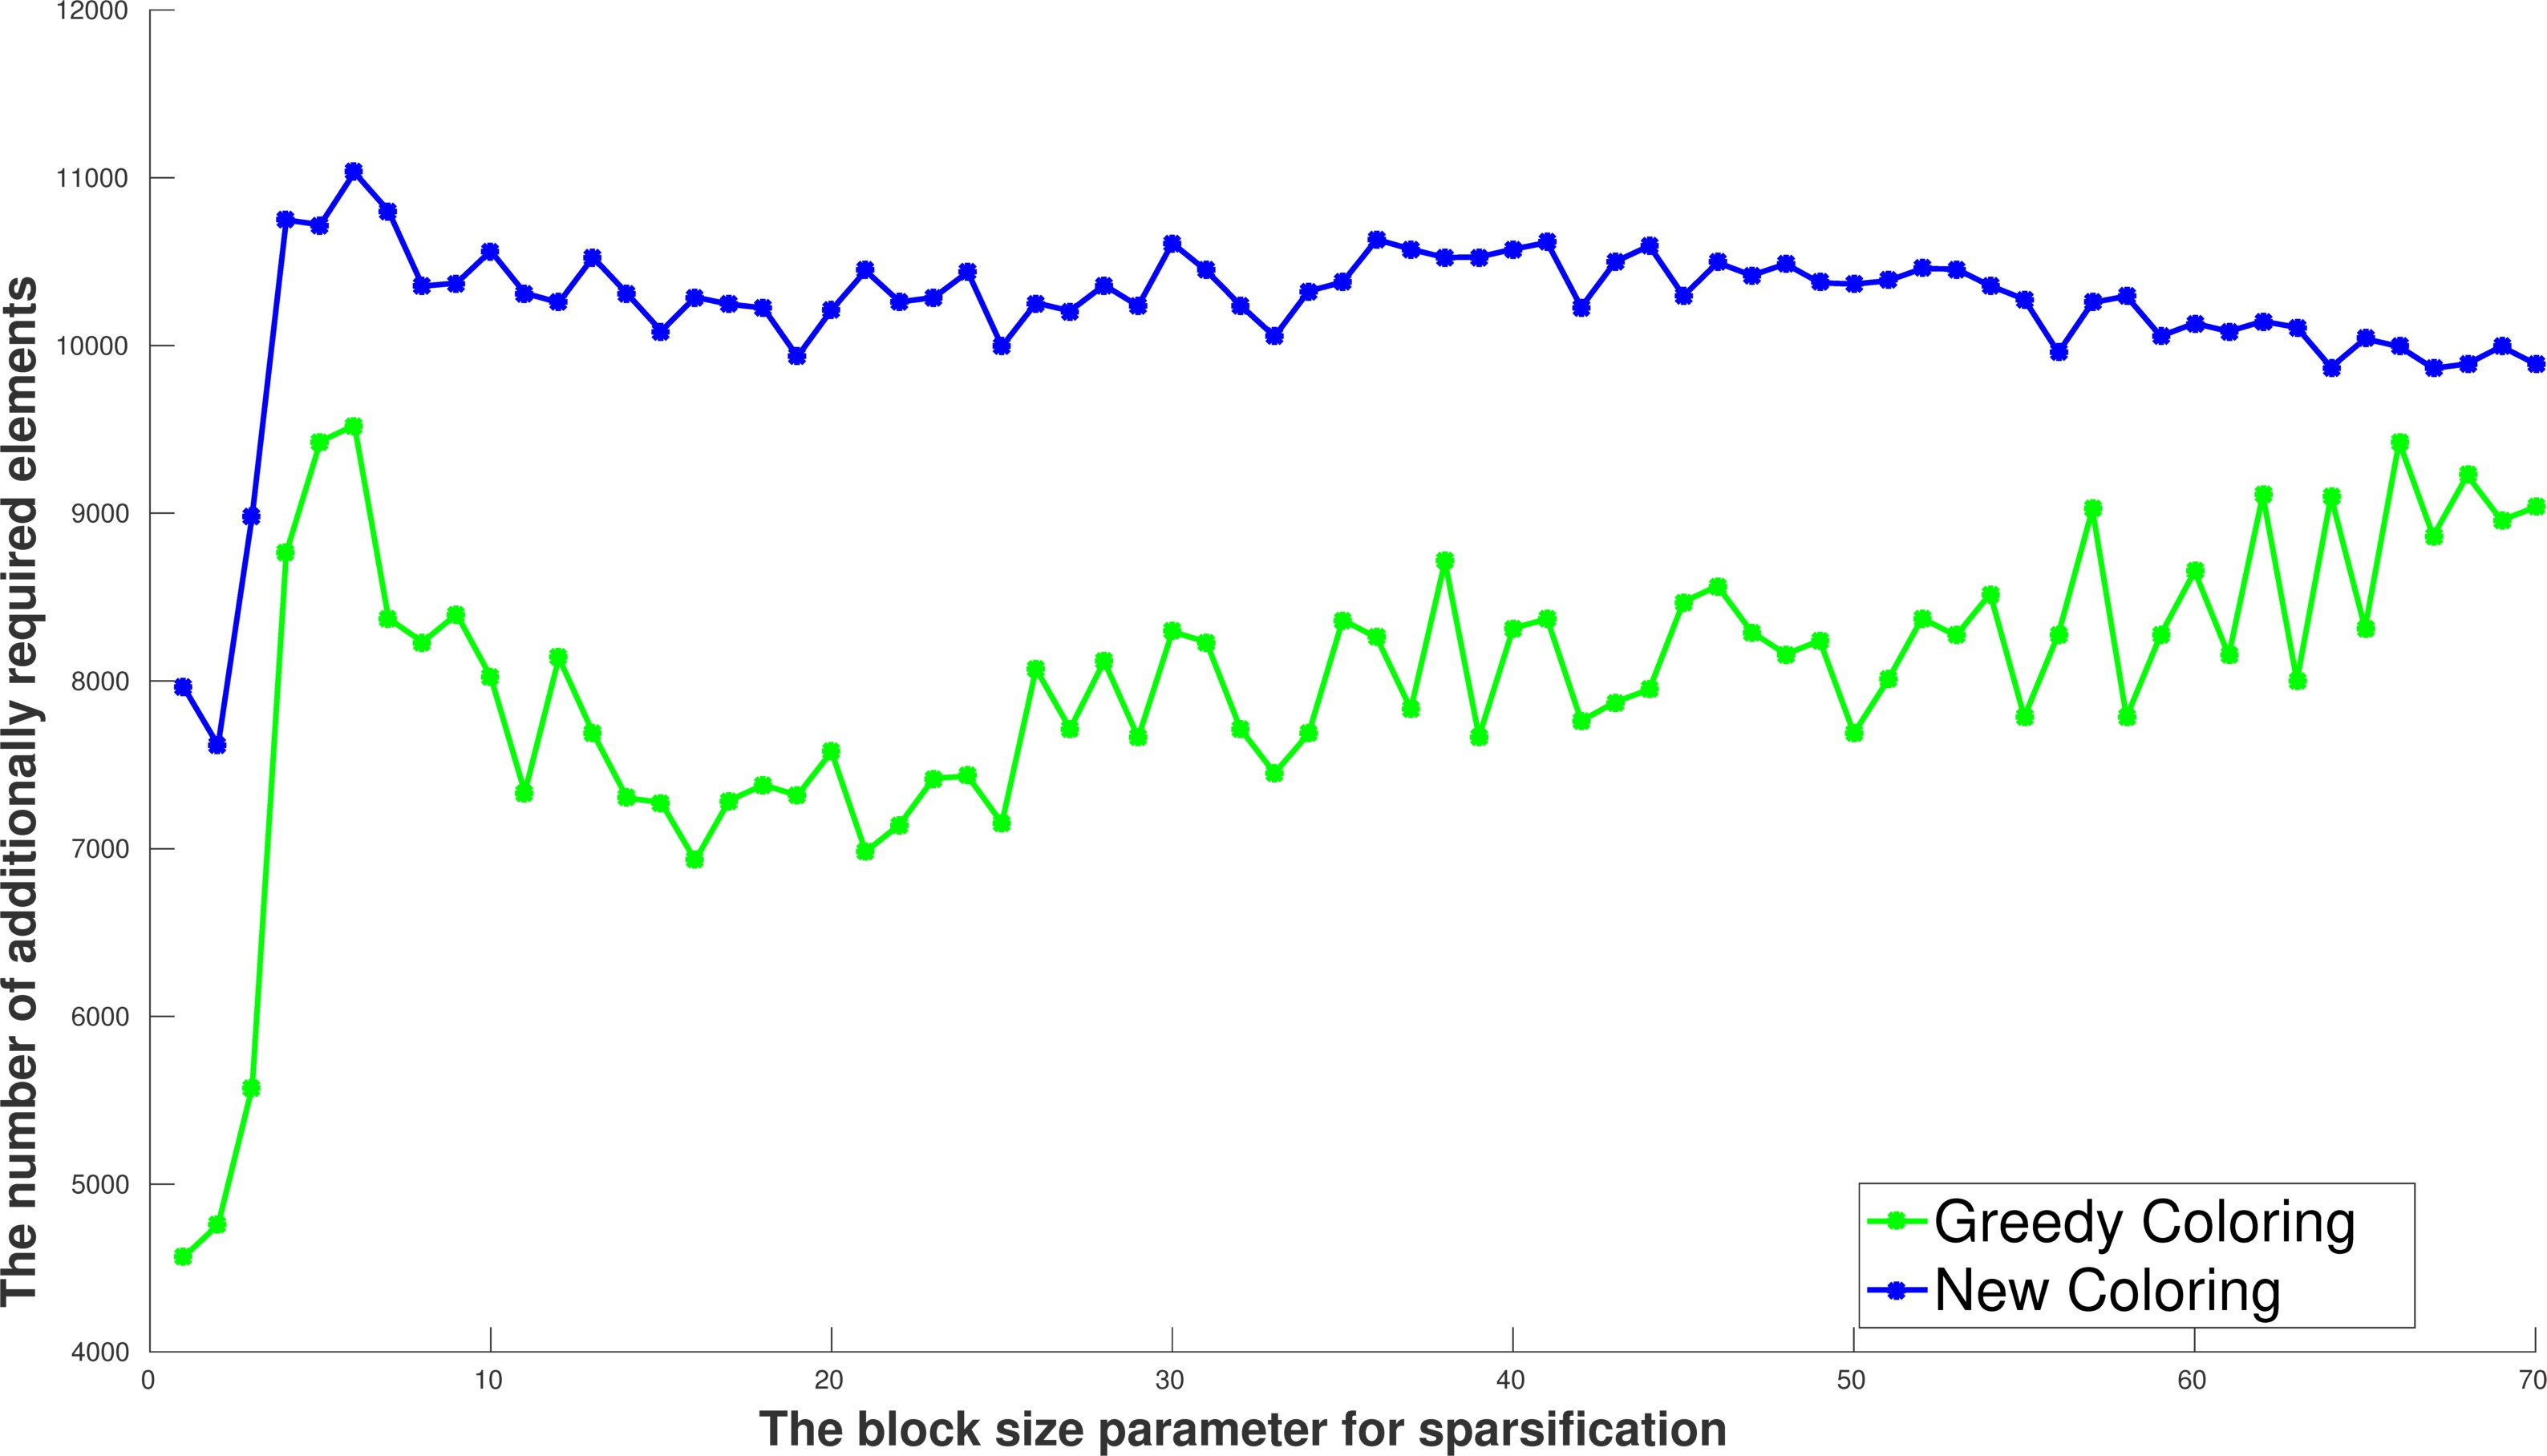
\includegraphics[width=0.9\linewidth]{bls_adds_ex33_without_alpha}
\caption{The number of colors in the new heuristic coloring compared with the greedy algorithm.
The computation is carried out on the matrix \textit{ex33}. }
\label{bls_adds_ex33_without_alpha}
\end{figure}

\begin{figure}
\centering
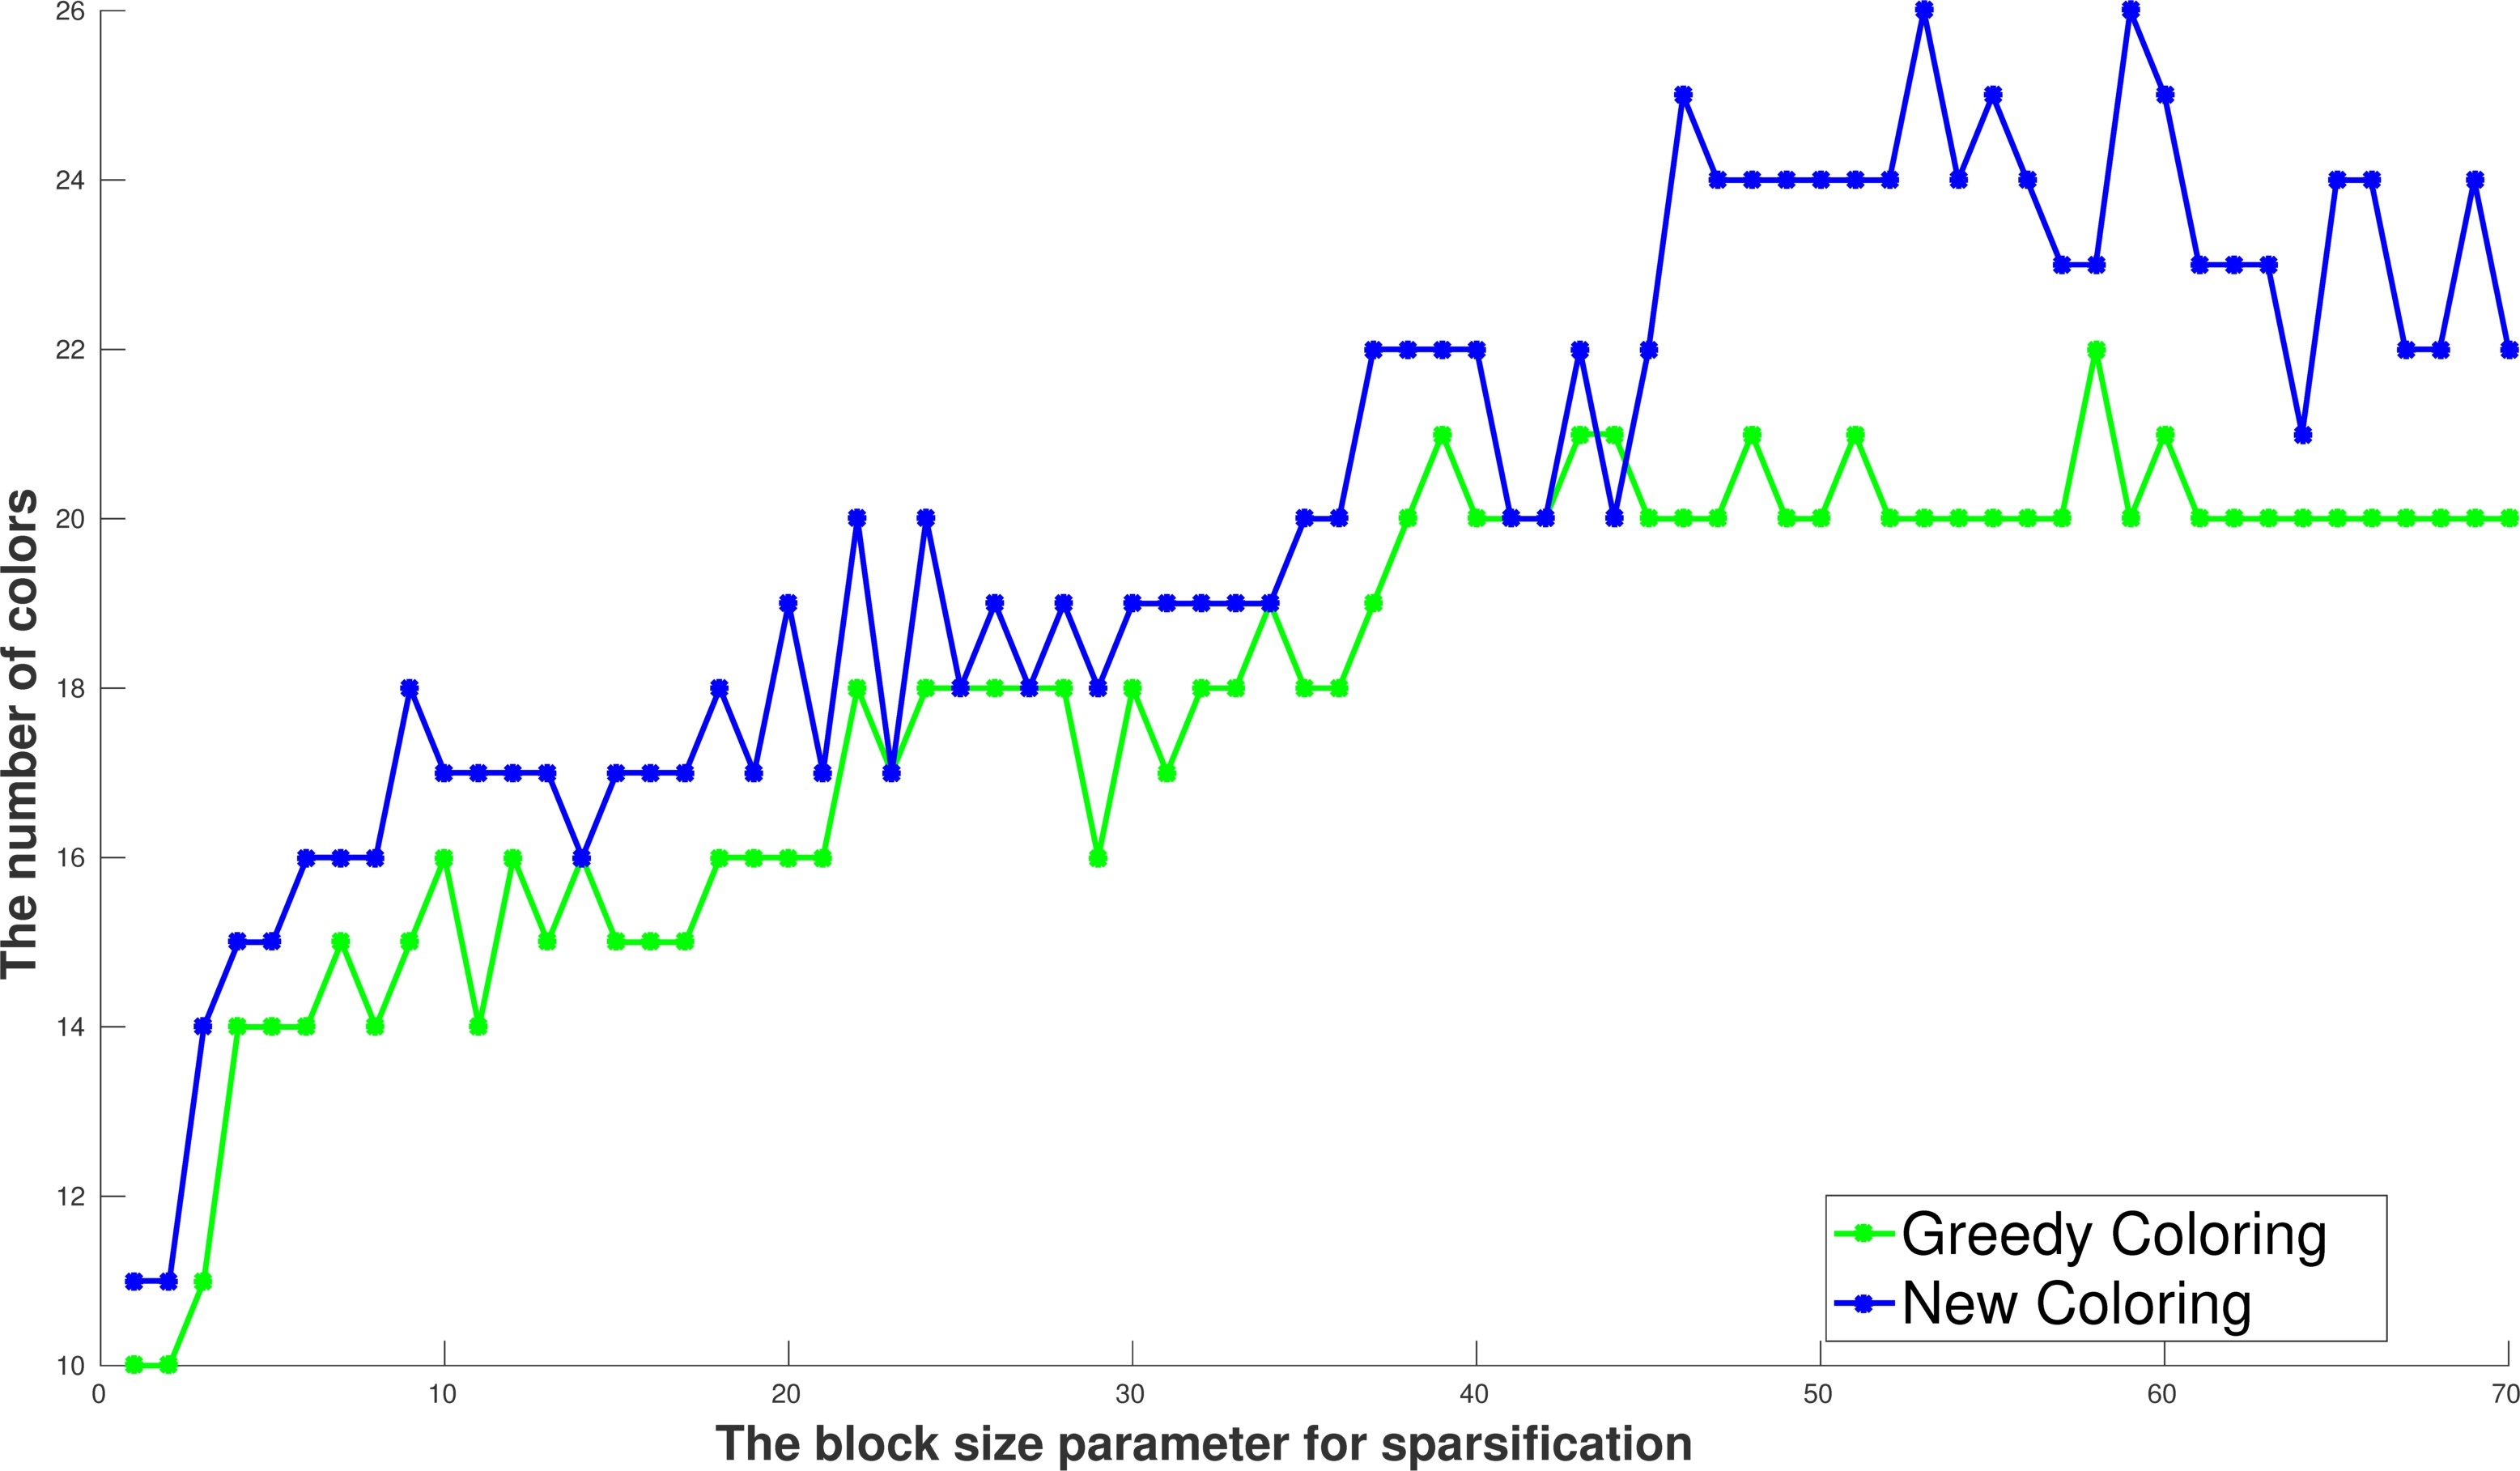
\includegraphics[width=0.9\linewidth]{bls_cols_ex33_without_alpha}
\caption{The number of additionally required elements in the new heuristic coloring compared with the greedy algorithm.
The computation is carried out on the matrix \textit{ex33}. }
\label{bls_cols_ex33_without_alpha}
\end{figure}
So far, we color a vertex with the maximum survived nonrequired elements.
However, it can happen
that we have more than one vertex with the maximum nonrequired elements in each step.
Suppose we are looking at the vertex $v$ and two vertices $a$ and $b$ have maximum values of
$Nreq(v,a) = Nreq(v,b)$.
It is not always the best decision
to color both vertices $a$ and $b$ in a step with the same color
because the value of $Nreq(a,b)$ can be very small and gives us smaller number
of potentially required elements (it can decrease the number of colors too).
So, a careful selection between computed set of vertices with the maximum number of
nonrequired elements would increase the potentiallye required elements without
any major changes in the structure of algorithm.
\begin{figure}
\begin{lstlisting}[
caption=A modification of the previous algorithm in which
a specific element is selected from the set of colums with
the maximum survived nonrequired elements.
we select only an arbitrary element in the previous version.,
label=code.new.impr1,mathescape]
function d2_color_nreq_modified($G=(V_r\cup V_c,E)$,$E_i\subset E$)
for $v\in V_c$
  $\Phi(v)=-1$
  $forbiddenColors[v] = 0$

for $v\in V_c$ with $\Phi(v)=0$
  $forbiddenColors[0] = v$
  if $\exists n\in N_2(v): (v,n)\in E_i$
    for $n\in N_2(v)$
      if $\Phi(n) \neq 0$
        $forbiddenColors[\Phi(n)] = v$

    $\Phi(v) = min \{ a>0:forbiddenColor[a]\neq v\}$
    $I_v=\{u\in V_c: u\notin N_2(v)\}$
    $M_1 = \{ (i,Nreq(i,v)): i\in I_v\}$
    $maxs = \{ a\in keys(M_1): M_1[a] = max(values(M_1))\}$
    $M_2 = \{ (i,req(i)): i\in maxs \}$
    $mins =\{ a\in keys(M_2): M_2[a] = min(values(M_2))\}$
    if(consistent($G$,$mins[0]$,$\Phi(v)$))
      $\Phi(mins[0]) = \Phi(v)$
\end{lstlisting}
\end{figure}

In \secref{s.max.add.req}, we will select those nonrequired elements which have more possibility
to be among the additionally required elements using the fill path theorem.
However, a first idea would be to select a vertex with the minimum number of required elements
among the computed set of vertices with the maximum number of nonrequired elements.
This facilitates gathering of more nonrequired elements in the same column since
it remains more free places for the other elements.

Let the function $Req(i)$ computes the number of required elements in the column $i$ or the
number of required edges which are neighbours of the vertex $i$,
we modify the previous algorithm as in \coderef{code.new.impr1} to
apply this idea. The set $M_1$ and $M_2\subset M_1$ contain the set of columns with the maximum
number of nonrequired elements and its subset with the minimal value of required elements.
The time complexity is still the same as \coderef{code.new.d2}
since only an additional part of sorting is computed.
\figref{bls_add_ex33_compare_max} shows how the number of additionally
required elements are increased comparing the new modified version with the previous strategy.
\begin{figure}
\centering
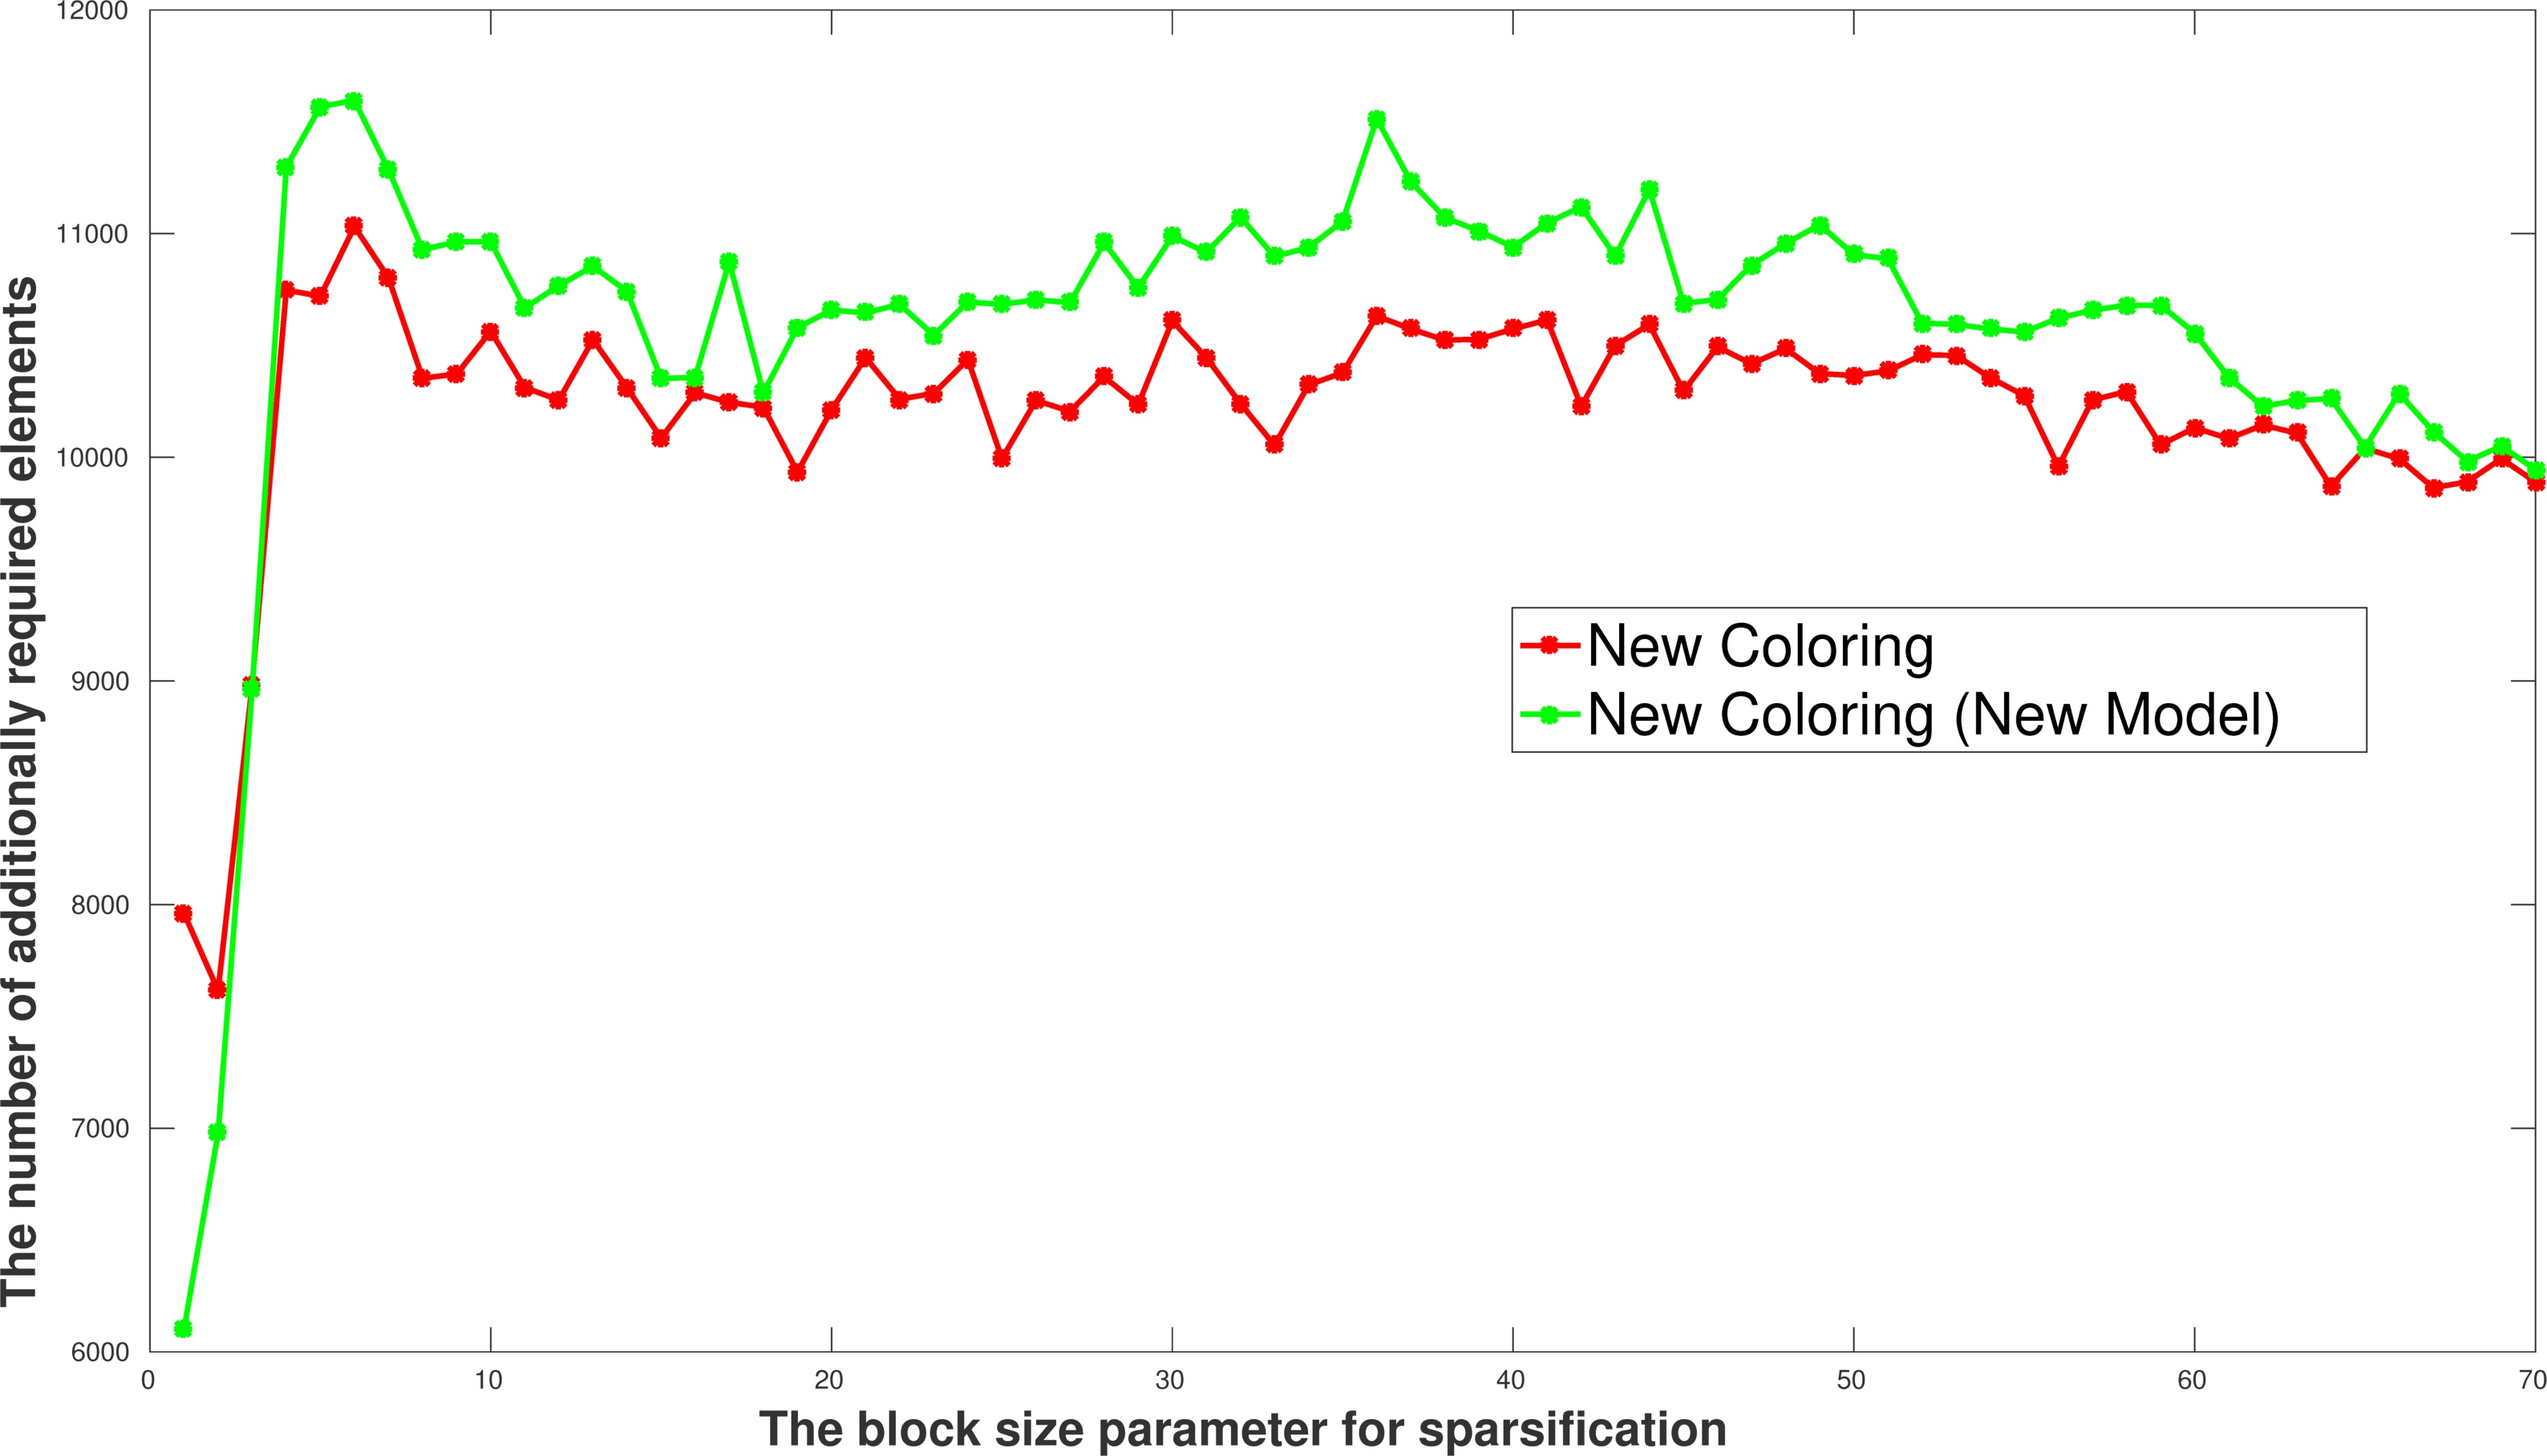
\includegraphics[width=0.9\linewidth]{bls_add_ex33_compare_max}
\caption{the number of additionally required elements are compared between the new heuristics
and the modified version.}
\label{bls_add_ex33_compare_max}
\end{figure}

Our algorithm is to color the columns such that the number of colors
remain almost the same while the number of additionally required elements are increased.
What if one can have some control over colors too.
A good heuristic for coloring is to color independent sets in each step.
For example, \figref{bls_cols_indset_ex33_} shows a comparison between a greedy algorithm and
an algorithm which colors the independent set first. As you can see the independent set algorithm
produces definitely less number of colors. However, it does not perform good in the case of additionally
required elements as in \figref{bls_adds_indset_ex33_}.

\begin{figure}
\centering
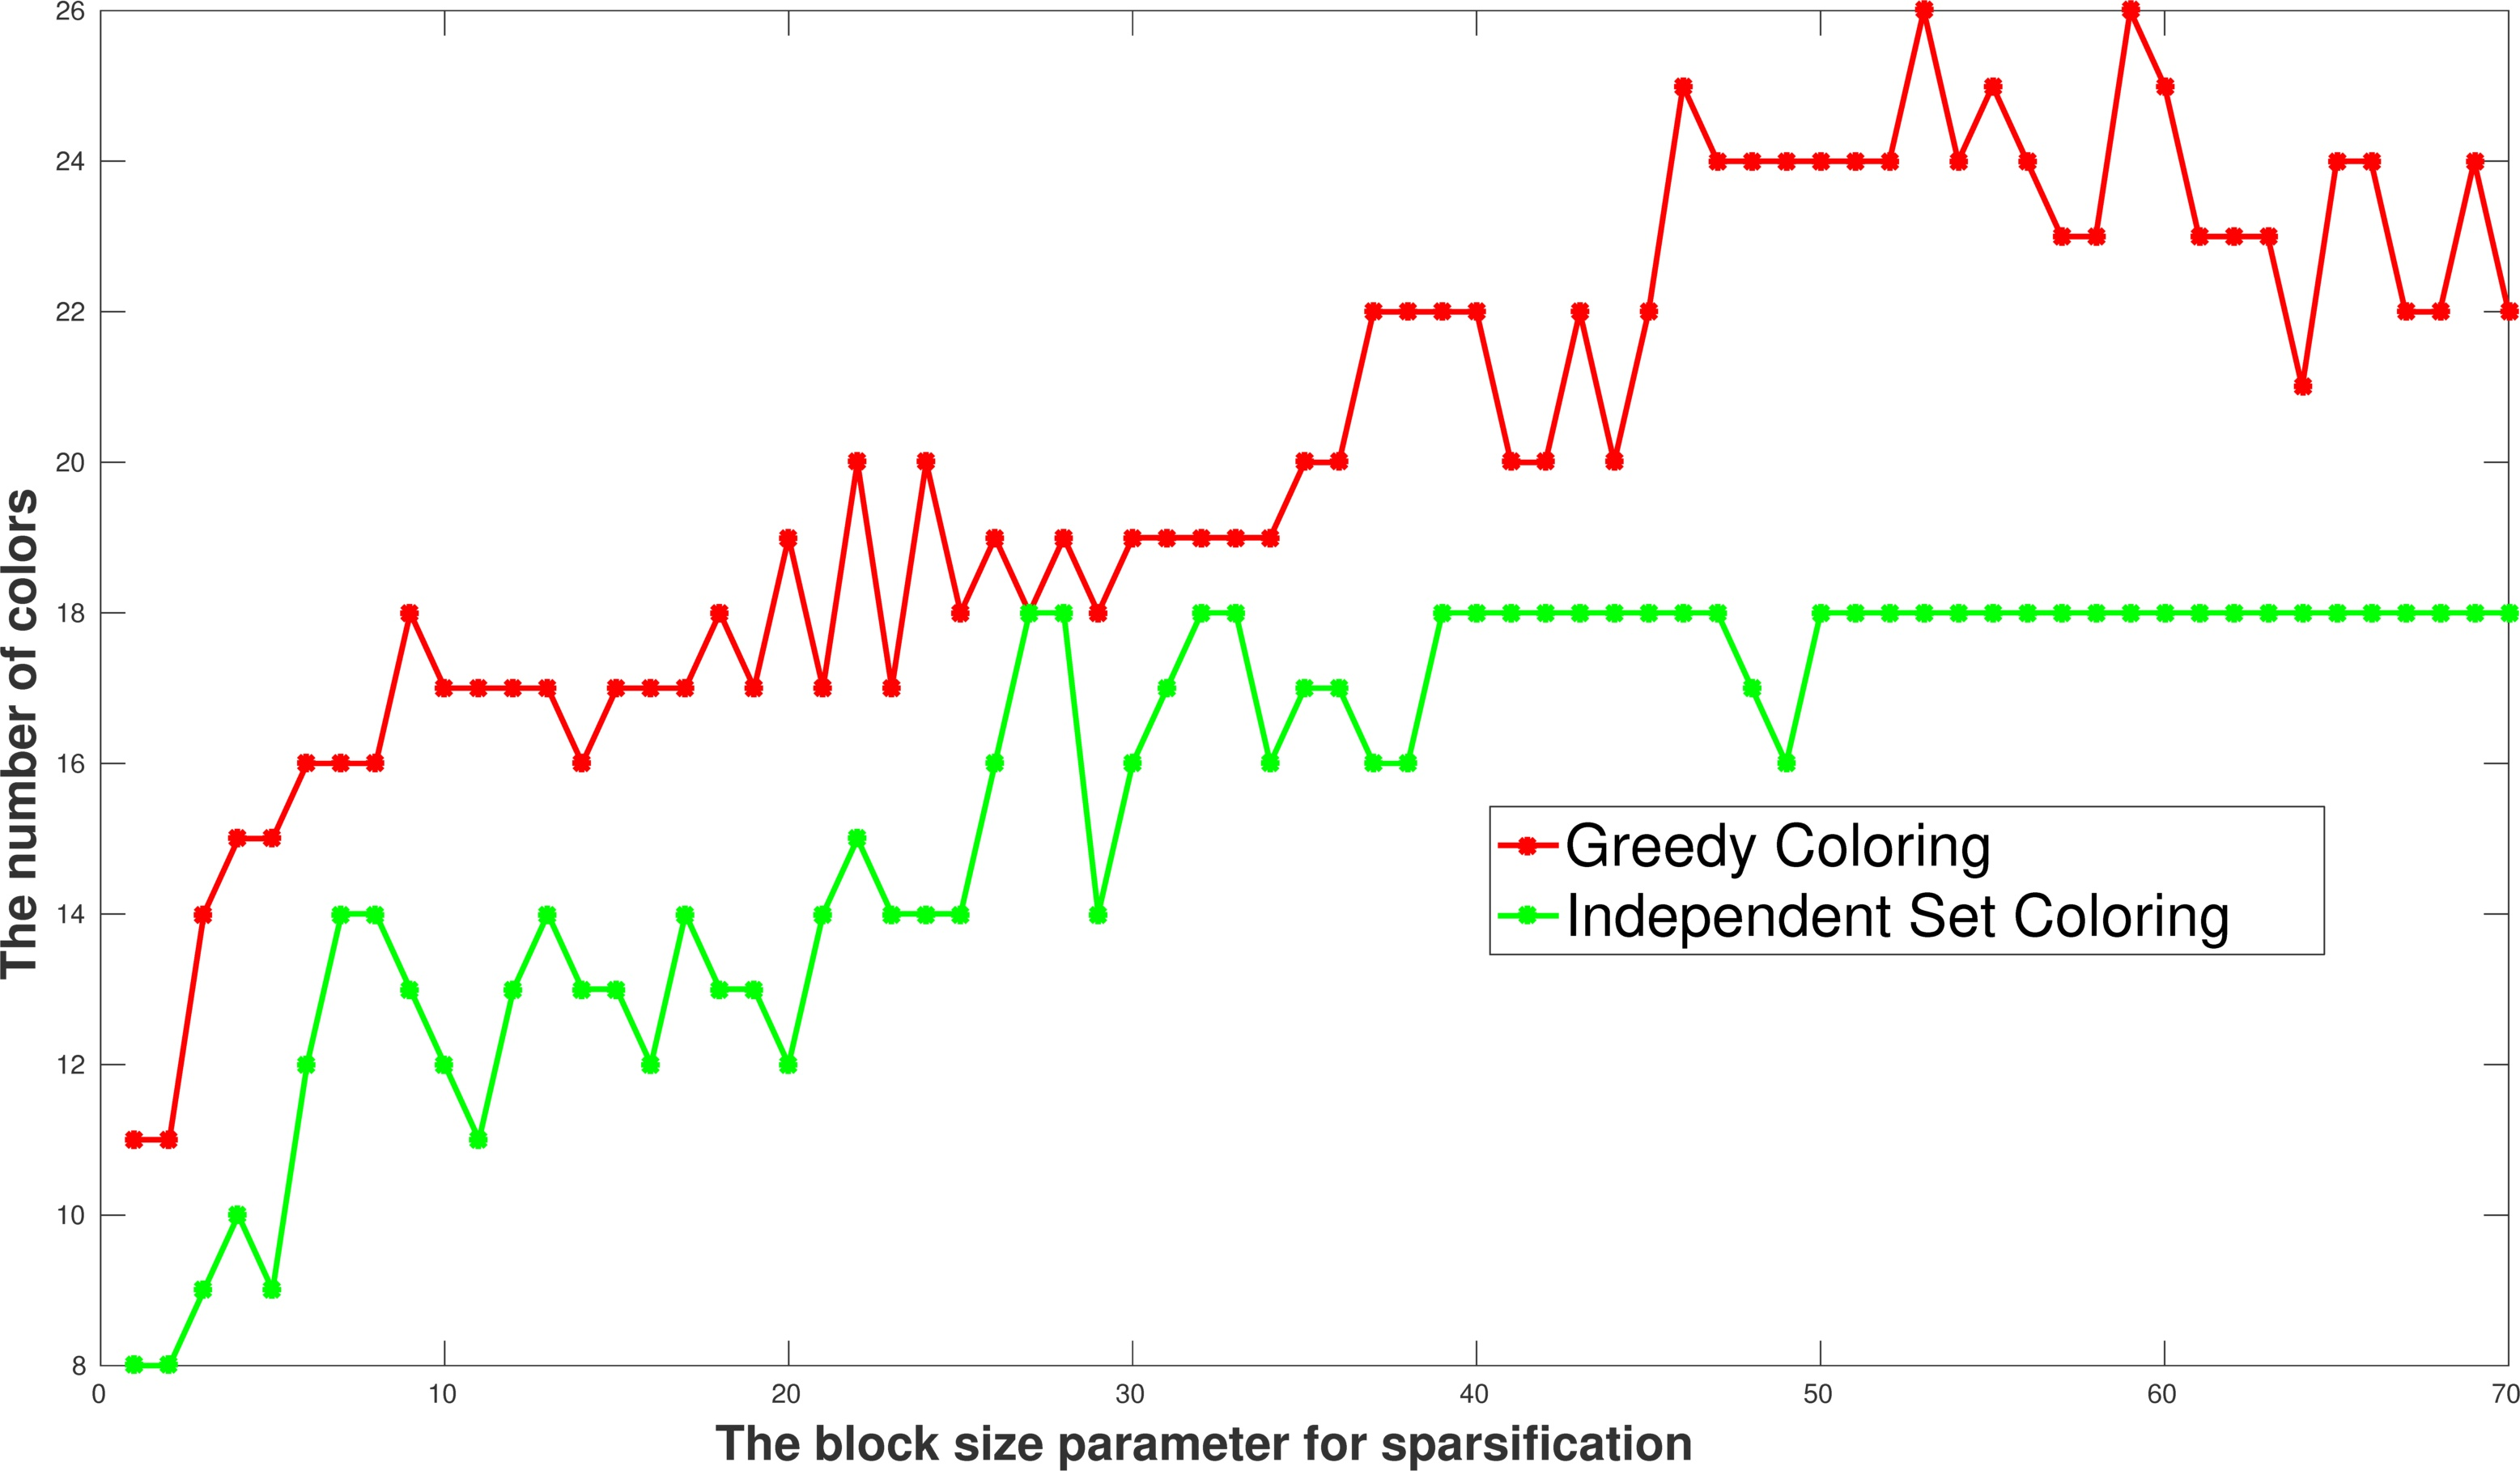
\includegraphics[width=0.9\linewidth]{bls_cols_indset_ex33_}
\caption{The comparison of an algorithm which color the independent sets first and
the greedy algorithm with respect to the number of colors.}
\label{bls_cols_indset_ex33_}
\end{figure}
\begin{figure}
\centering
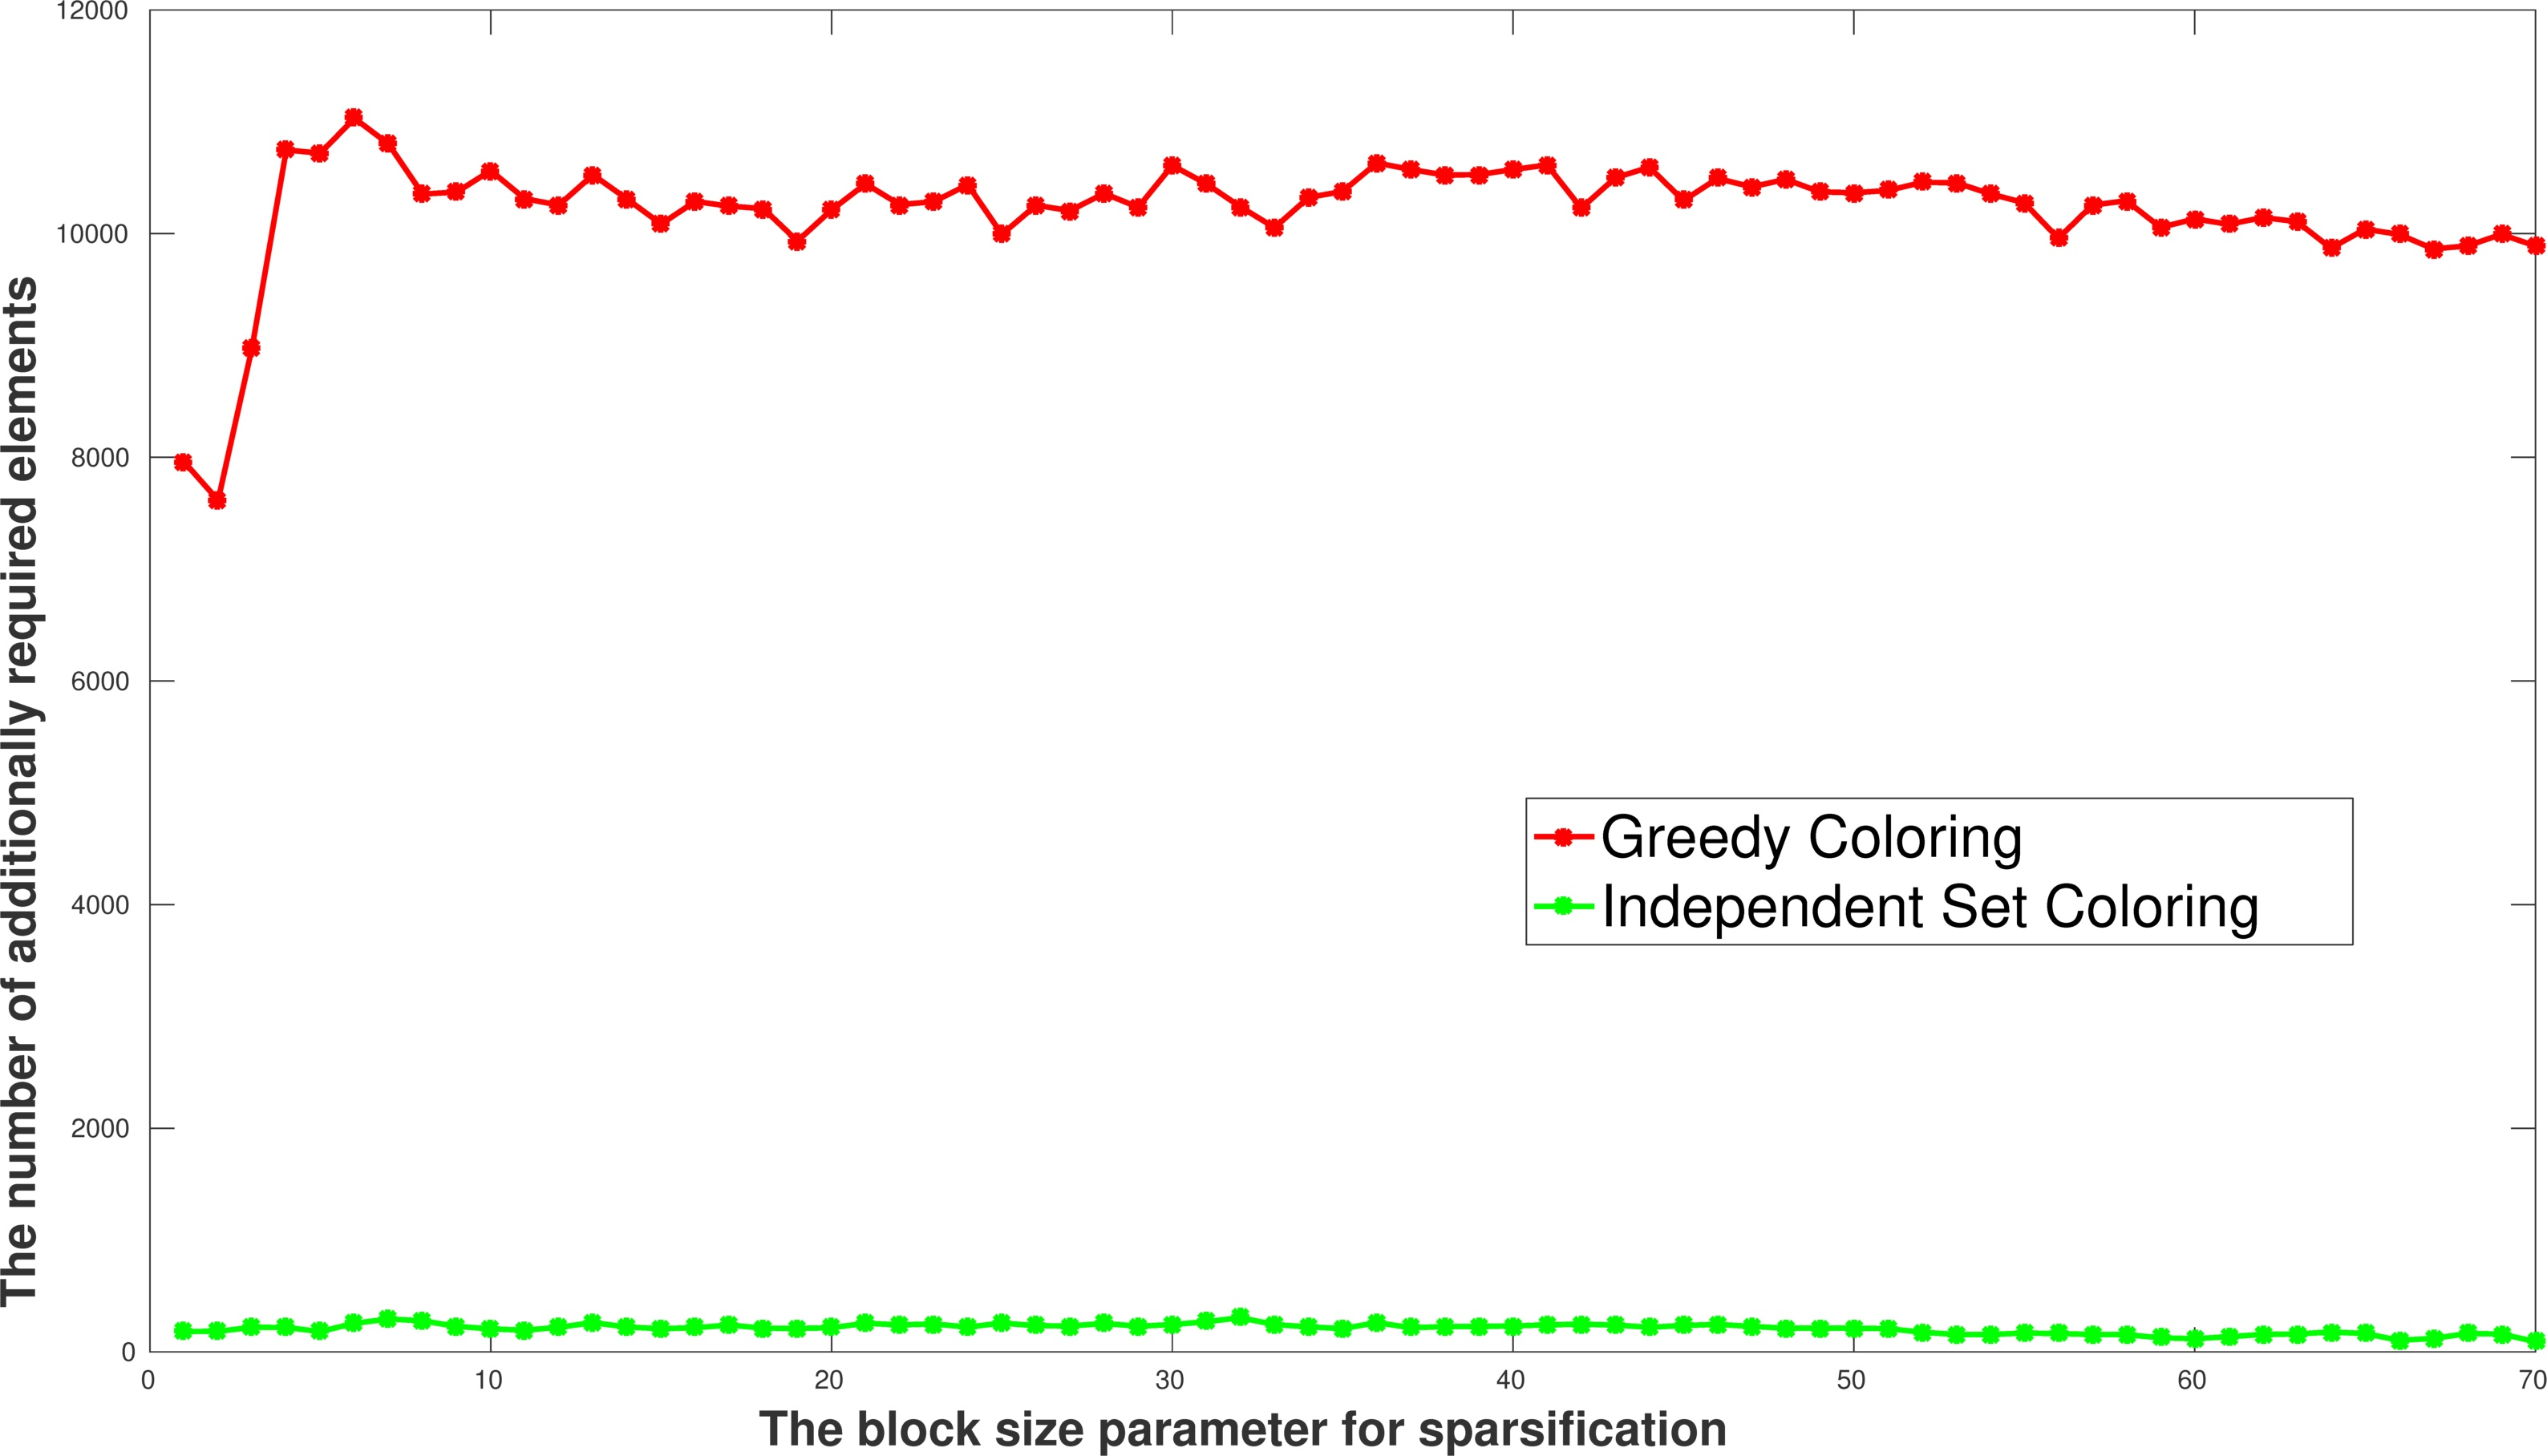
\includegraphics[width=0.9\linewidth]{bls_adds_indset_ex33_}
\caption{The comparison of an algorithm which color the independent sets first and
the greedy algorithm with respect to the number of additionally required elements.}
\label{bls_adds_indset_ex33_}
\end{figure}

It is a logical result since we saw that selecting two columns with the maximum number of nonrequired
elements does not give us always more number of additionally required elements.
So, we propose to choose only column with the maximum number of nonrequired elements and
choose $\alpha$ other columns with the minimum number of nonrequired elements. In this case,
we can decrease the number of colors by increasing the value $\alpha$ while the number of
additionally required elements decrease only a little bit.
The new star bicoloring algorithm is as \coderef{code.new.impr2}.
\begin{figure}
\begin{lstlisting}[
caption=New coloring heuristc with a controller to balance
the number of colors and the number of additionally required elements.,
label=code.new.impr2,mathescape]
function d2_color_nreq_balance($G=(V_r\cup V_c,E)$,$E_i\subset E$,$\alpha$)
for $v\in V_c$
  $\Phi(v)=-1$
  $forbiddenColors[v] = 0$

for $v\in V_c$ with $\Phi(v)=0$
  $forbiddenColors[0] = v$
  if $\exists n\in N_2(v): (v,n)\in E_i$
    for $n\in N_2(v)$
      if $\Phi(n) \neq 0$
        $forbiddenColors[\Phi(n)] = v$

    $\Phi(v) = min \{ a>0:forbiddenColor[a]\neq v\}$
    $I_v=\{u\in V_c: u\notin N_2(v)\}$
    $M_1 = \{ (i,Nreq(i,v)): i\in I_v\}$
    $maxs = \{ a\in keys(M_1): M_1[a] = max(values(M_1))\}$
    $M_2 = \{ (i,req(i)): i\in maxs \}$
    $mins =\{ a\in keys(M_2): M_2[a] = min(values(M_2))\}$
    if(consistent($G$,$mins[0]$,$\Phi(v)$))
      $\Phi(mins[0]) = \Phi(v)$
    for $i\in\{0,1,...,\alpha\}$
      if(consistent($G$,$mins[i]$,$\Phi(v)$))
        $\Phi(mins[i]) = \Phi(v)$
\end{lstlisting}
\end{figure}

So if we choose $\alpha=0$, we would have the same algorithm as before.
As in~\figref{new.col.add.alpha.zero}, the number of additionally required elements
would increase. The number of colors is almost in the same order as in~\figref{new.col.col.alpha.zero}.
It can be compared to the computation on the same configuration but with different $\alpha=6$.
The number of colors would increase as in~\figref{new.col.col.alpha.six} while
the number of additionally required elements would not decrease a lot as in~\figref{new.col.col.alpha.six}.
\begin{figure}
\centering
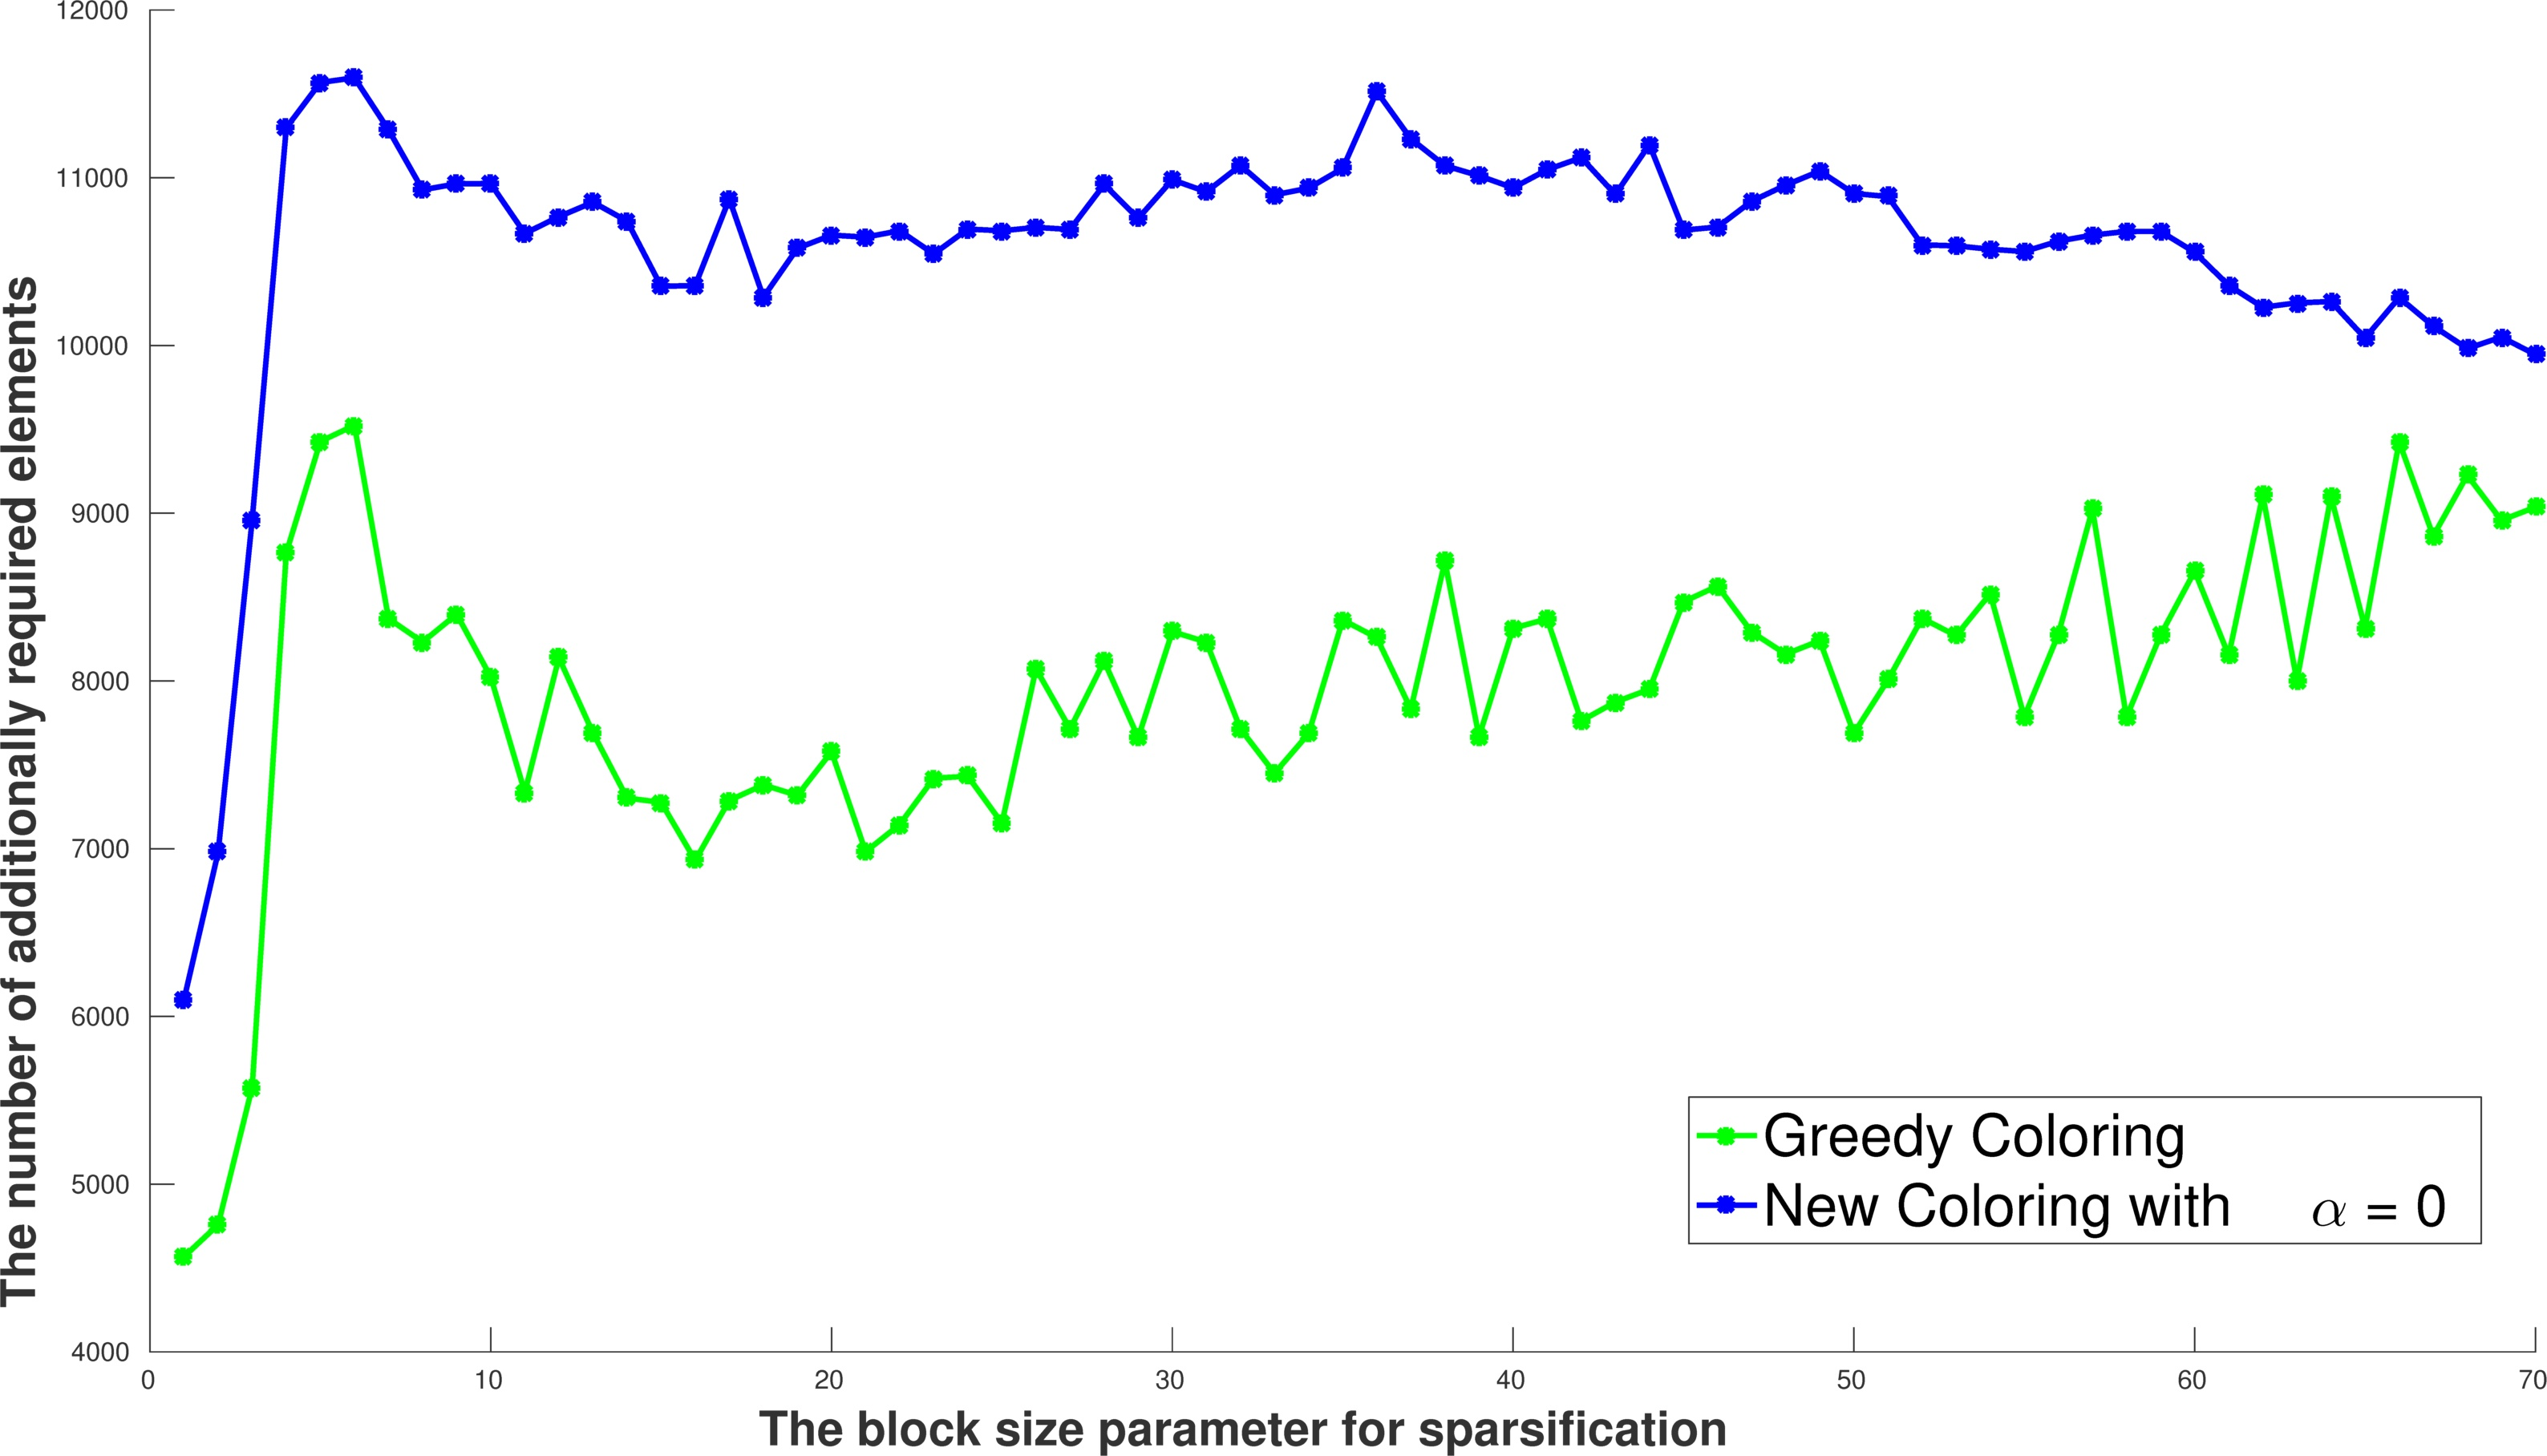
\includegraphics[width=0.9\linewidth]{bls_add_alpha_0}
\caption{The number of additionally required elements computed by the new heuristics compared with the
greedy algorithm. The computation carried out on the matrix \textit{ex33} and value of $\alpha$ is
set to $0$.}
\label{new.col.add.alpha.zero}
\end{figure}
\begin{figure}
\centering
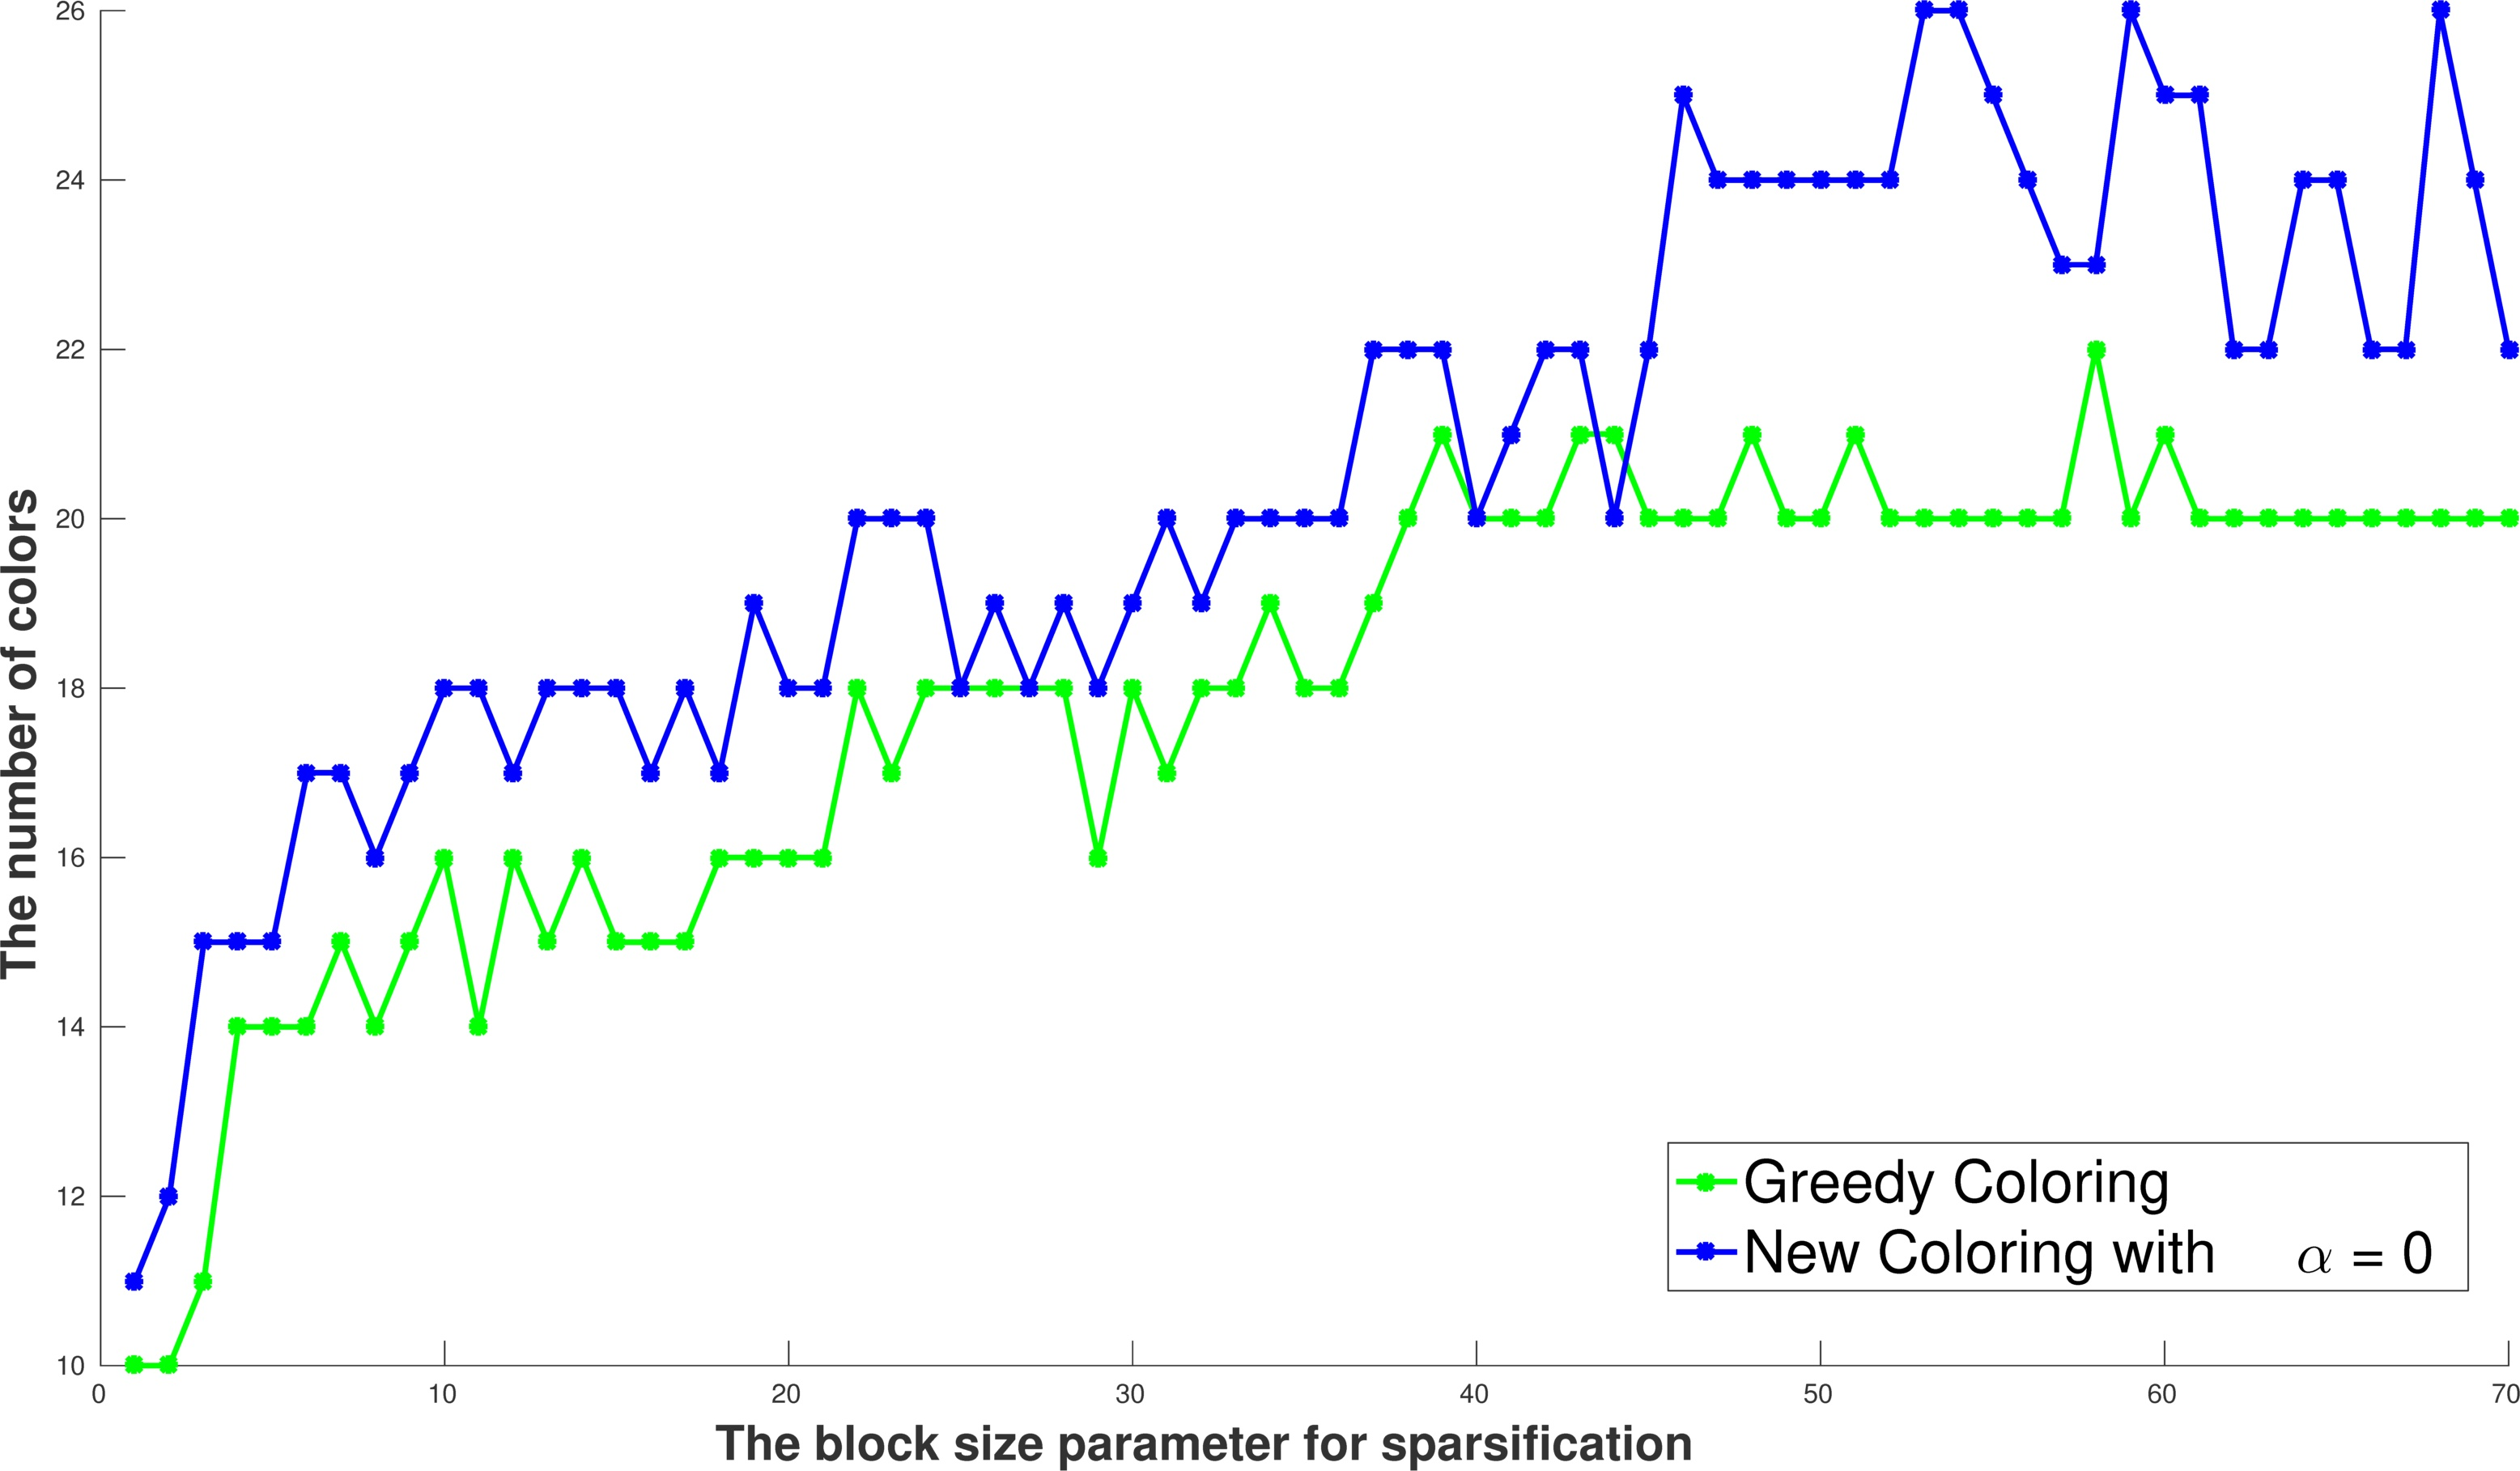
\includegraphics[width=0.9\linewidth]{bls_col_alpha_0}
\caption{The number of colors computed by the new heuristics compared with the
greedy algorithm. The computation carried out on the matrix \textit{ex33} and value of $\alpha$ is
set to $0$.}
\label{new.col.col.alpha.zero}
\end{figure}

\begin{figure}
\centering
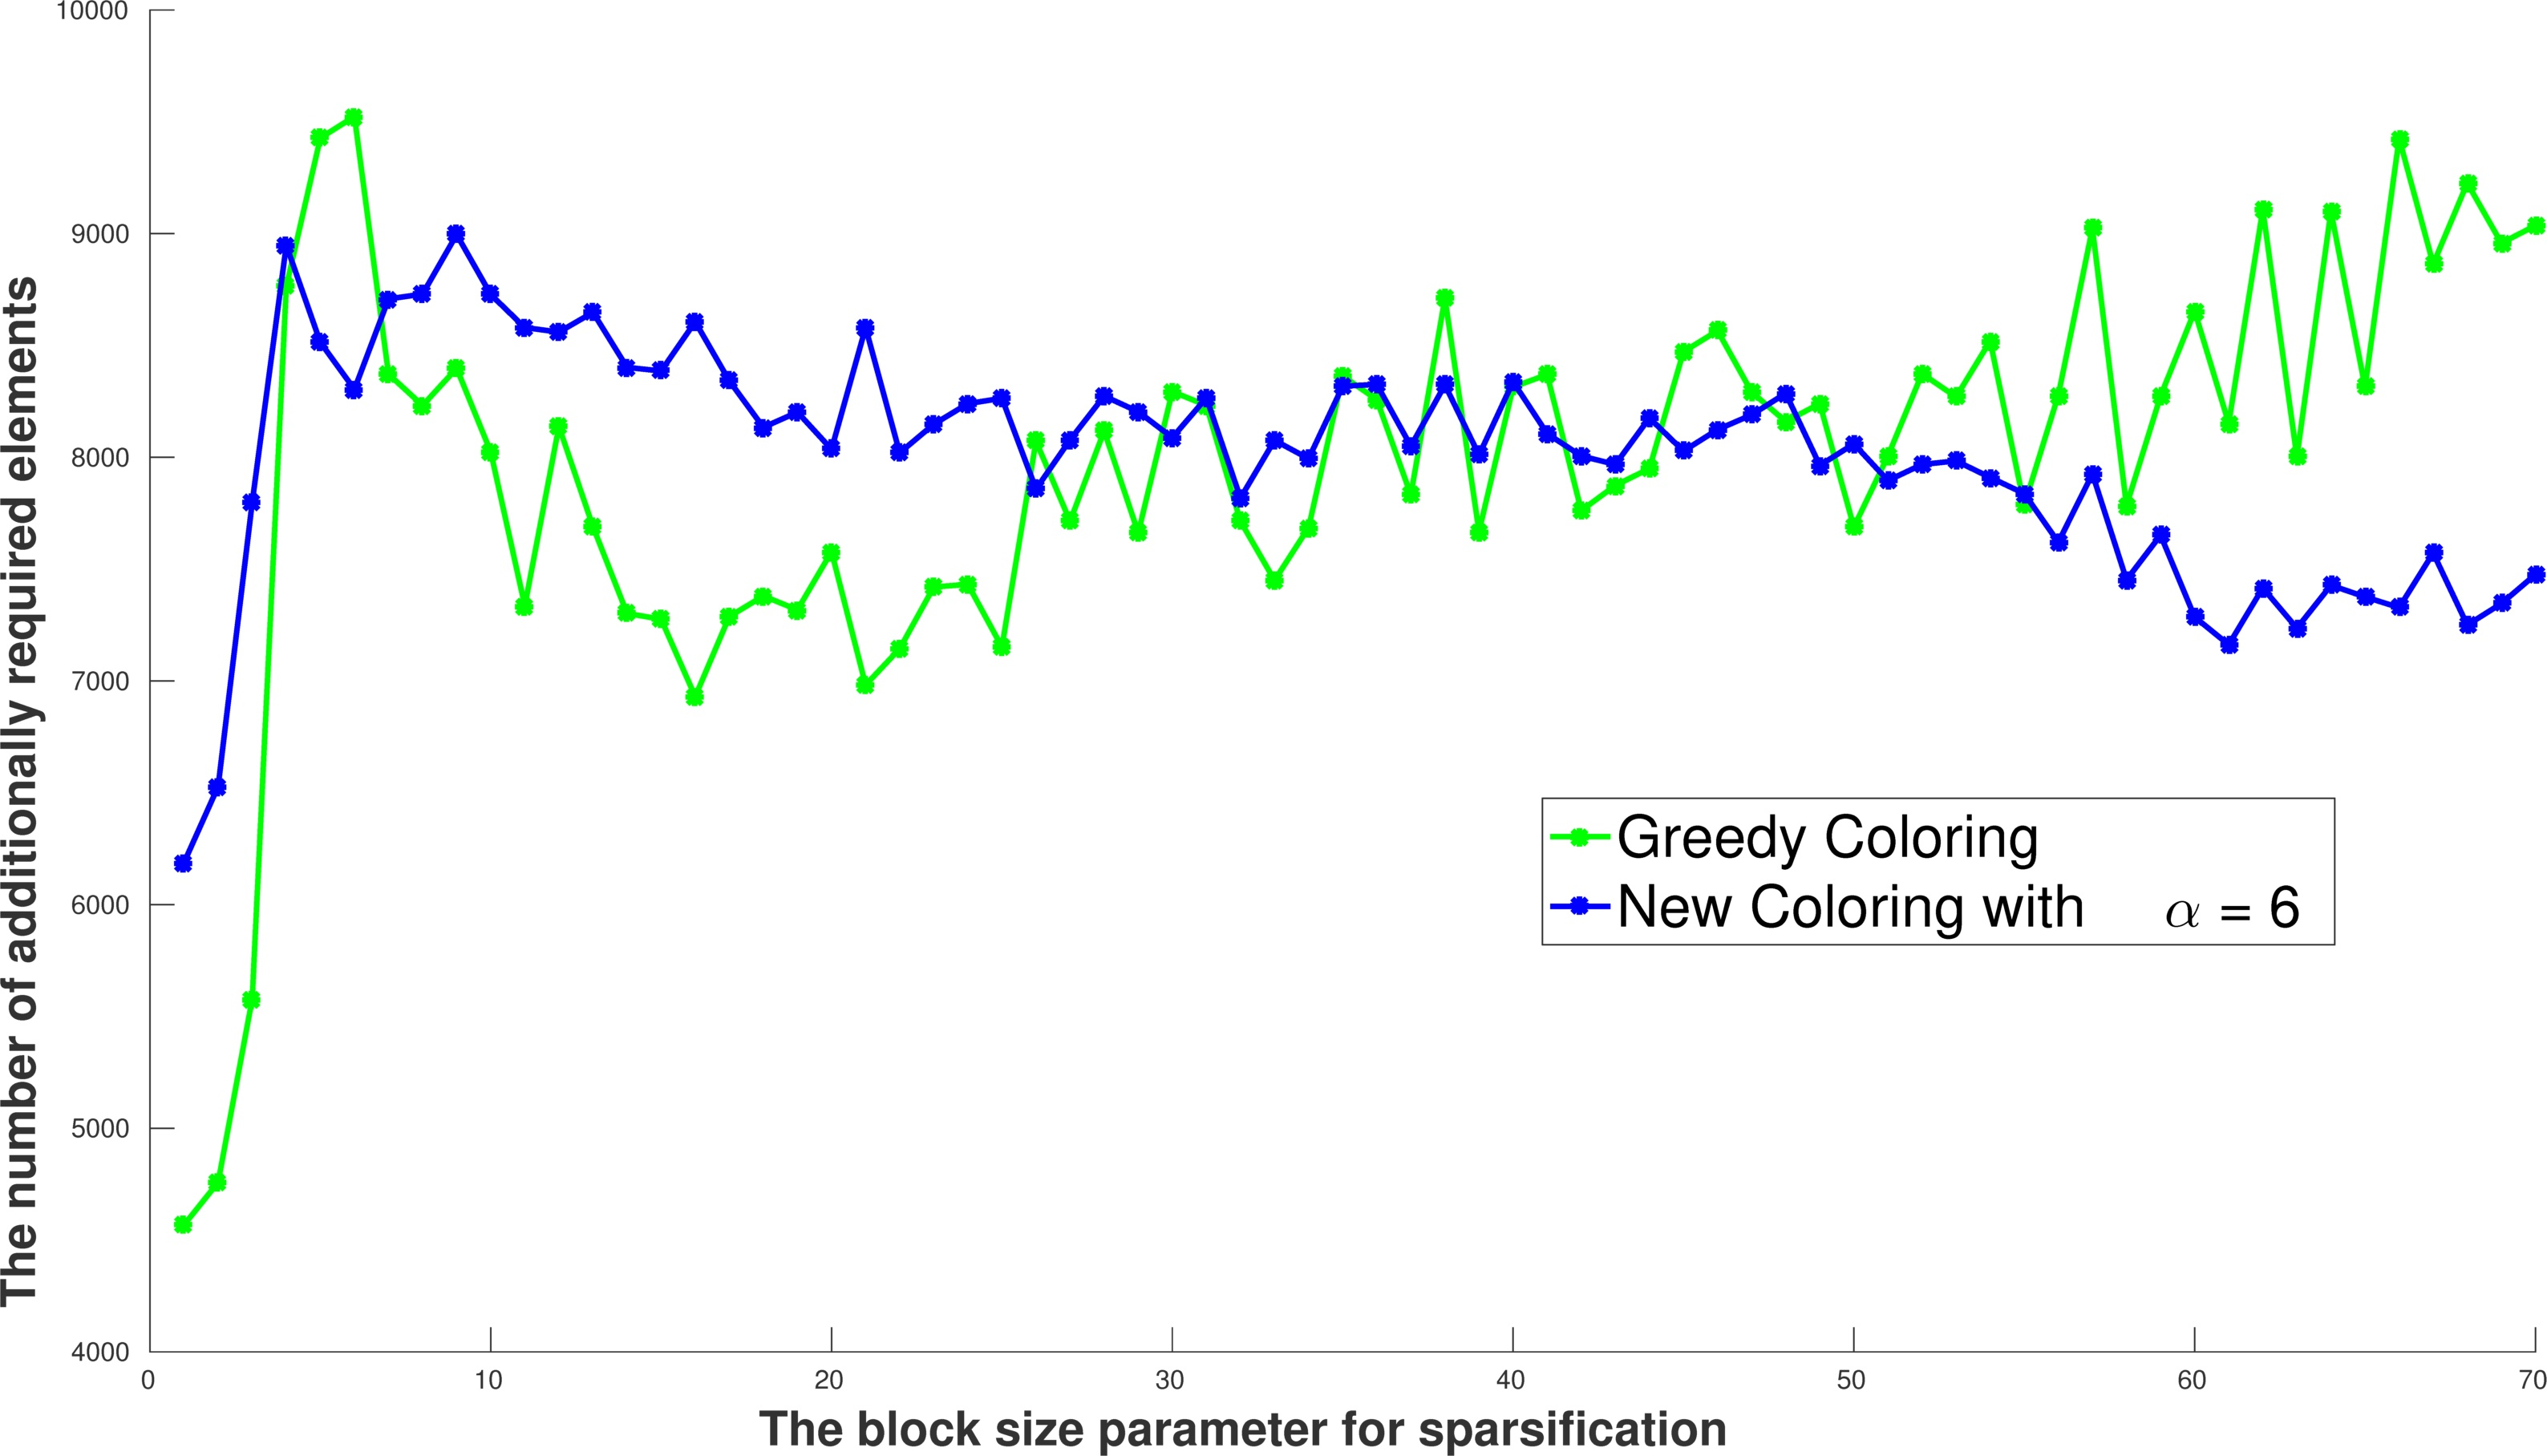
\includegraphics[width=0.9\linewidth]{bls_add_alpha_6}
\caption{The number of additionally required elements computed by the new heuristics compared with the
greedy algorithm. The computation carried out on the matrix \textit{ex33} and value of $\alpha$ is
set to $6$.}
\label{new.col.add.alpha.six}
\end{figure}
\begin{figure}
\centering
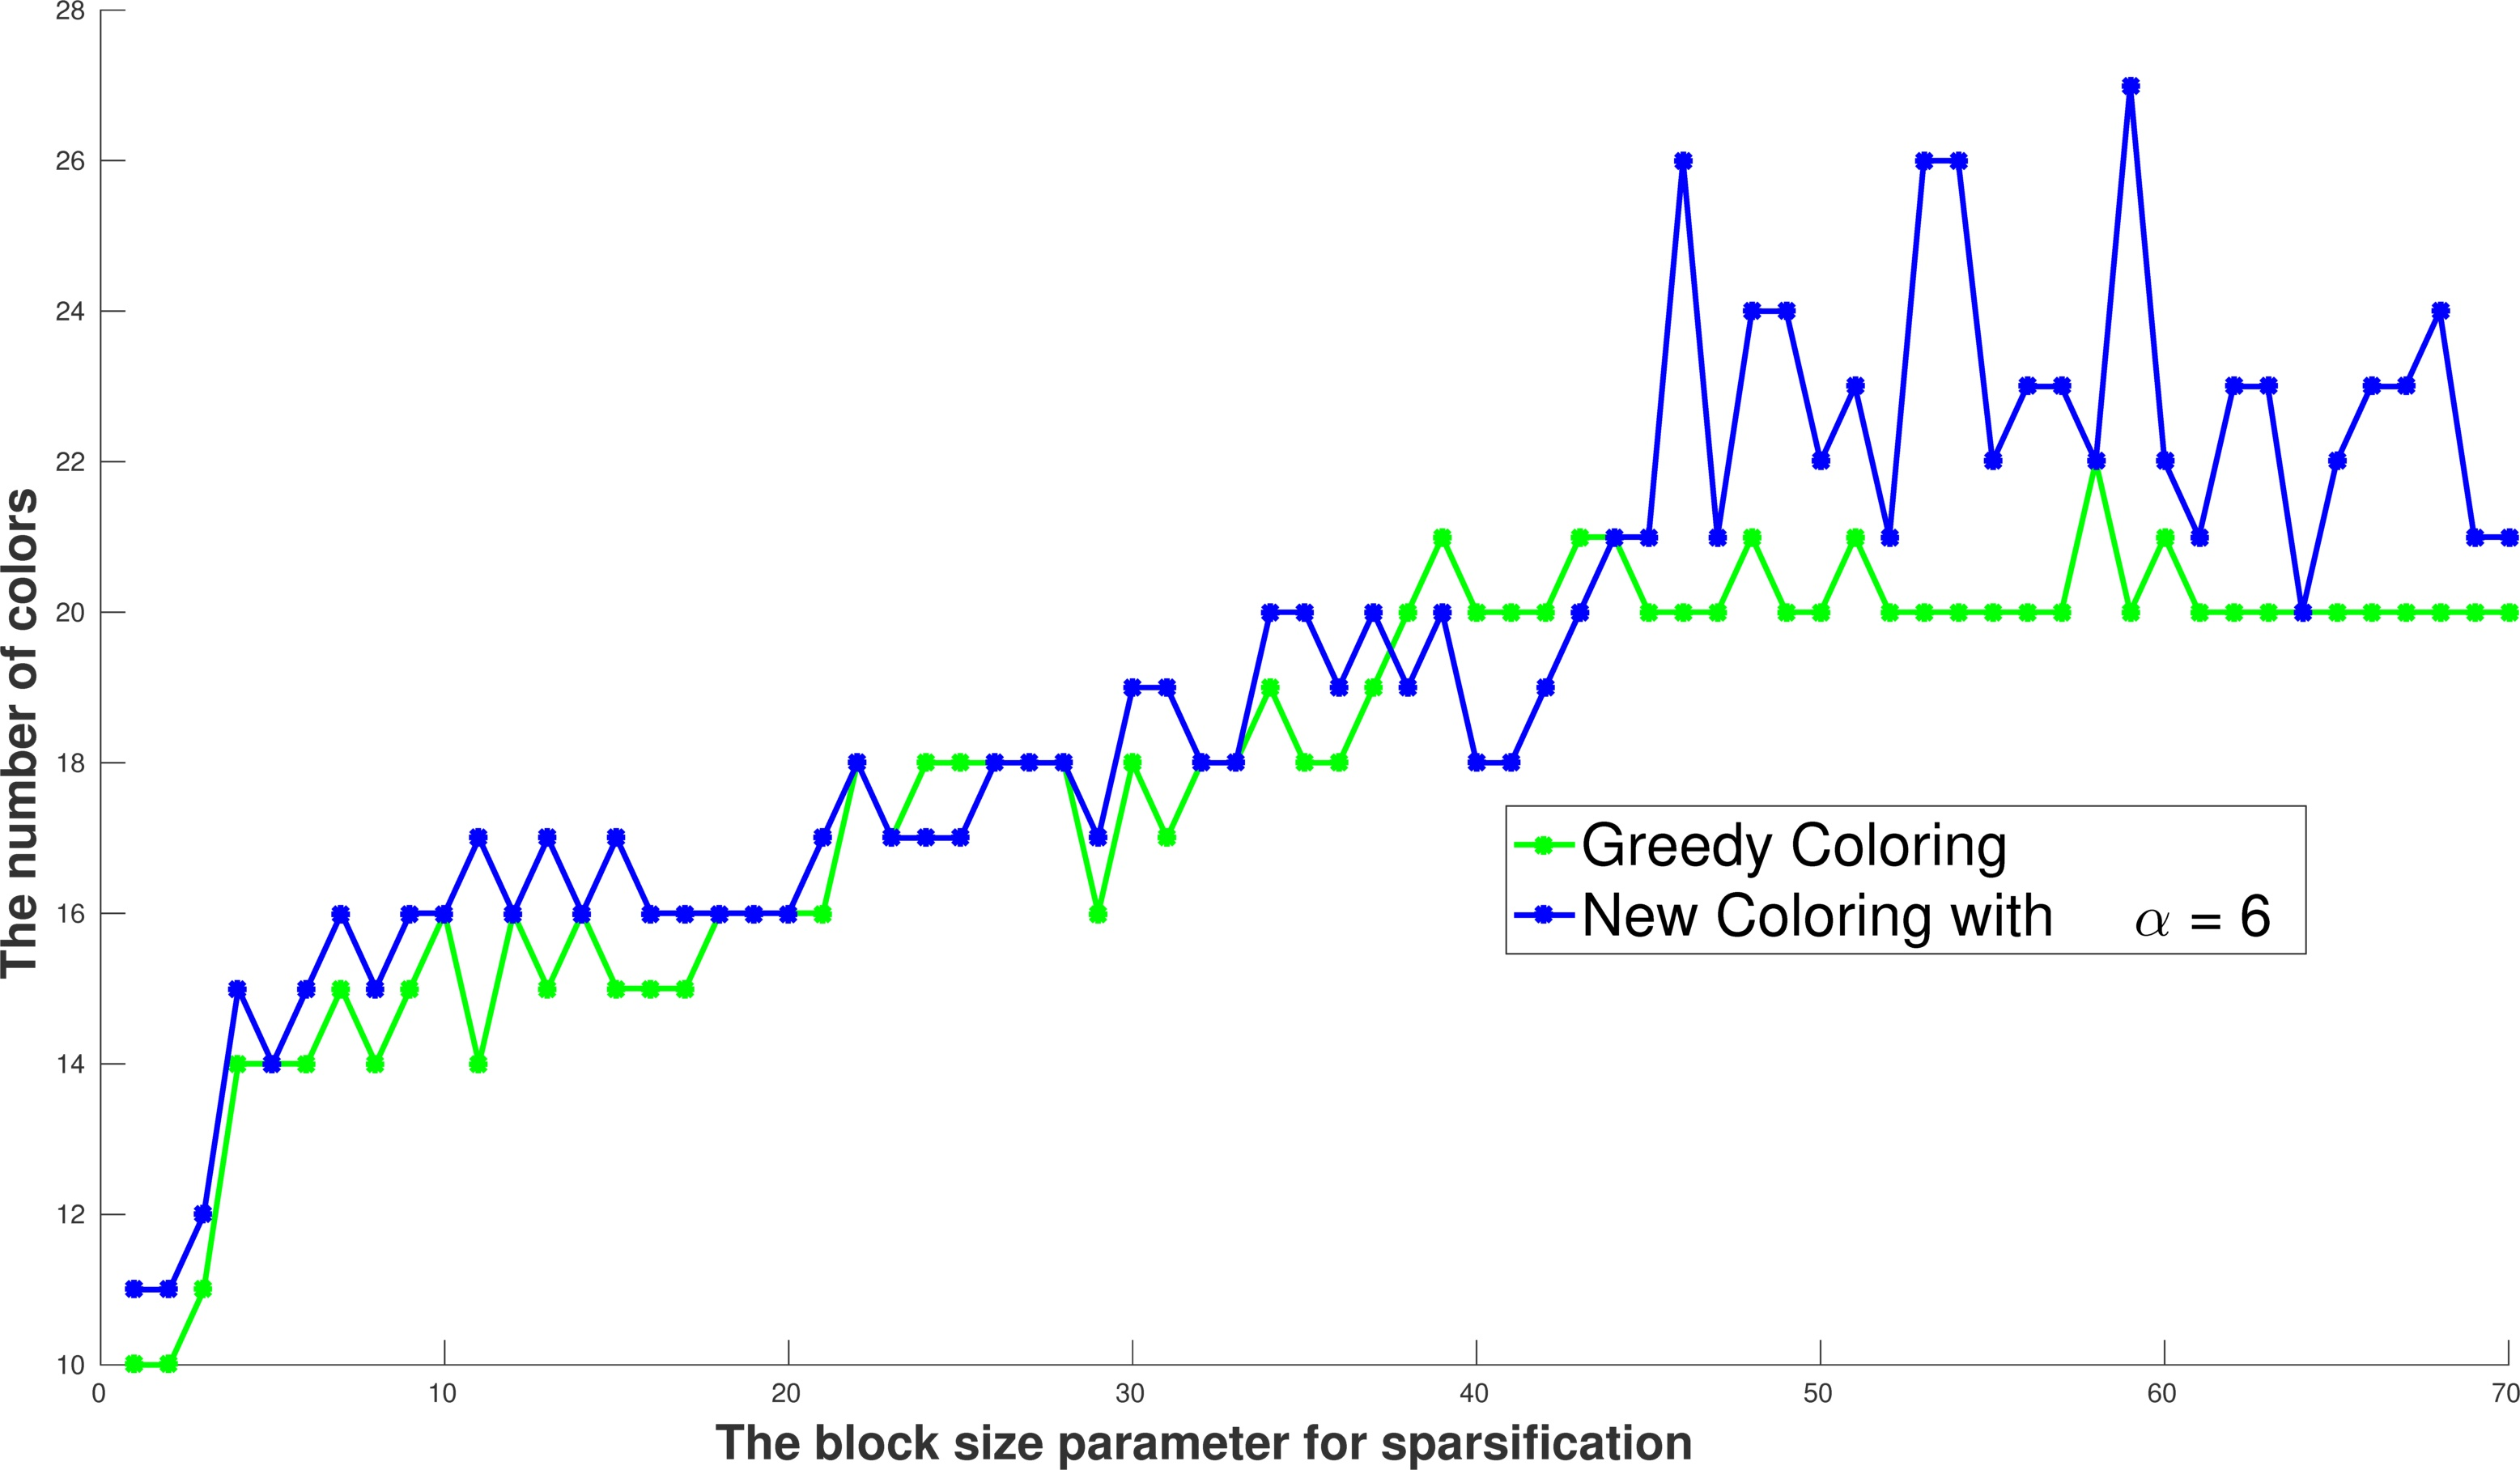
\includegraphics[width=0.9\linewidth]{bls_col_alpha_6}
\caption{The number of colors computed by the new heuristics compared with the
greedy algorithm. The computation carried out on the matrix \textit{ex33} and value of $\alpha$ is
set to $6$.}
\label{new.col.col.alpha.six}
\end{figure}

Here, we compute the new heuristic on the other matrix \textit{nos3}
and the results for $\alpha=10$ are shown in~\figref{new.col.add.alpha.ten.nos3}
and~\figref{new.col.col.alpha.ten.nos3}
and for $\alpha=1$ are shown in~\figref{new.col.add.alpha.one.nos3} and
in~\figref{new.col.col.alpha.one.nos3}.
The new computations shows almost the same results. However,
the only difference is that all the results change dramatically
after the size of block $40$. In general, an observation can be
summarized that the results are better than for the smaller size of blocks
specially when the matrix is small.

\begin{figure}
\centering
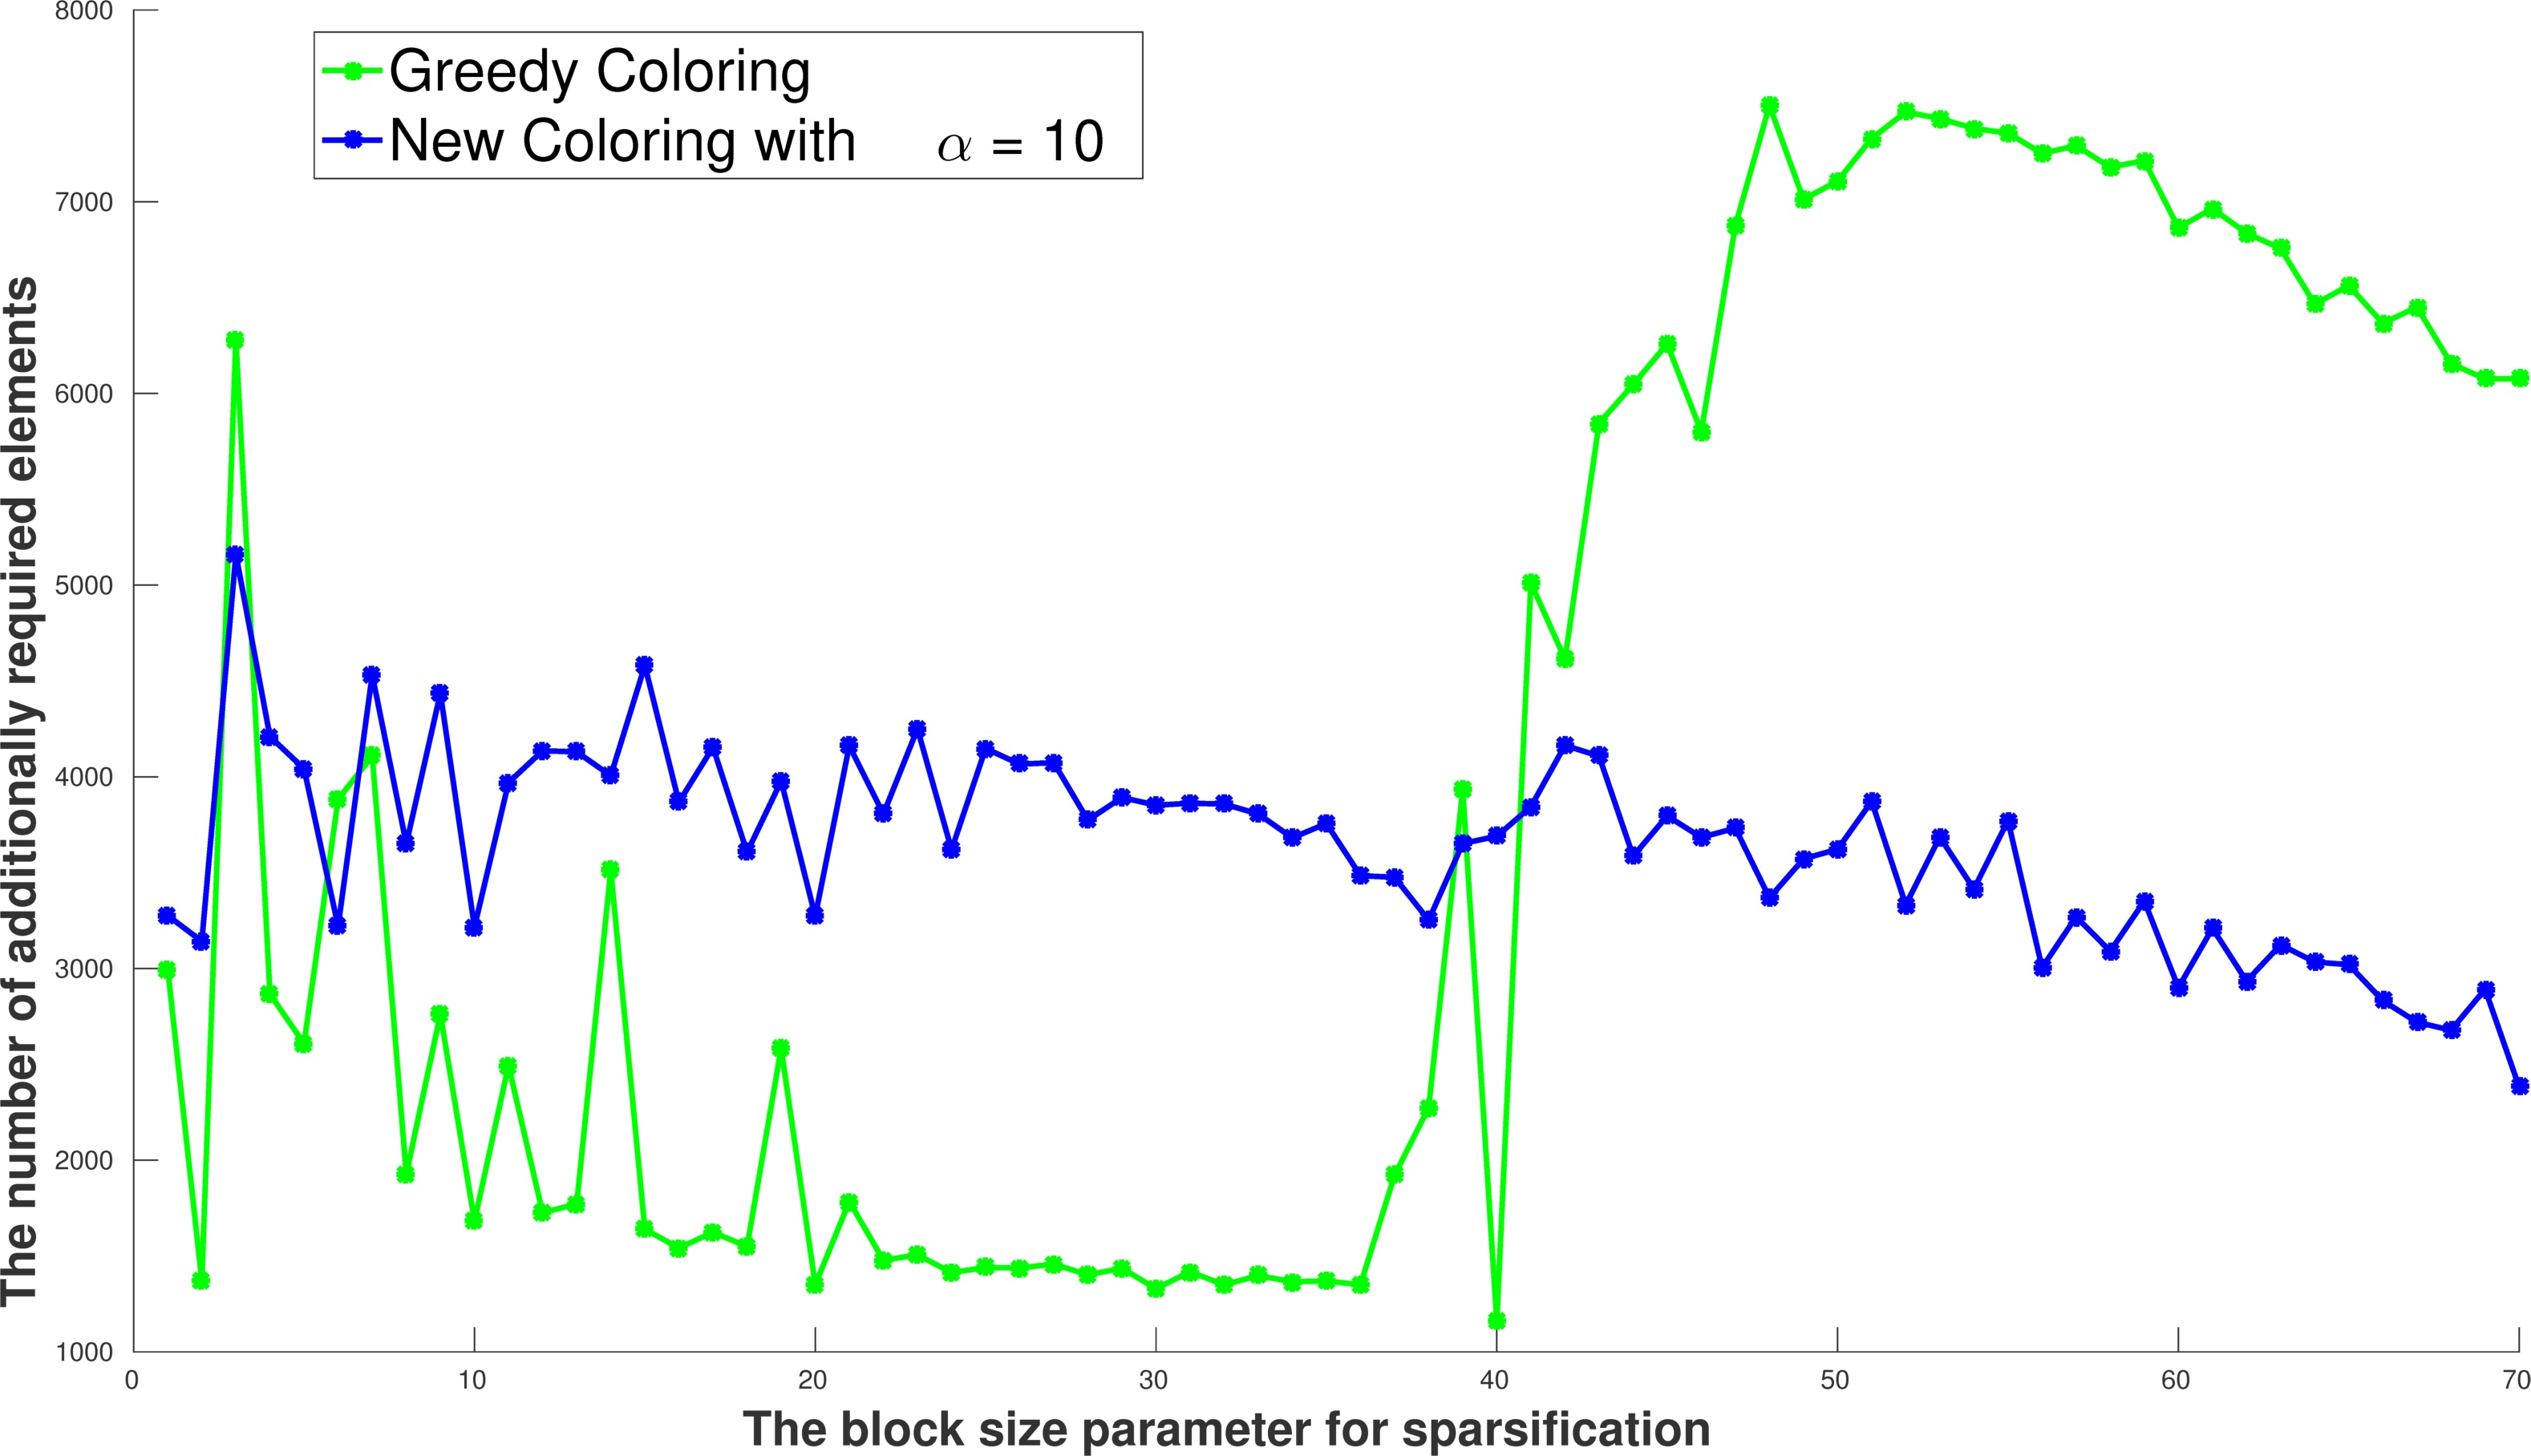
\includegraphics[width=0.9\linewidth]{bls_add_alpha_10_nos3}
\caption{The number of additionally required elements computed
by the new heuristics compared with the greedy algorithm.
The computation carried out on the matrix \textit{nos3}
and value of $\alpha$ is set to $10$.}
\label{new.col.add.alpha.ten.nos3}
\end{figure}
\begin{figure}
\centering
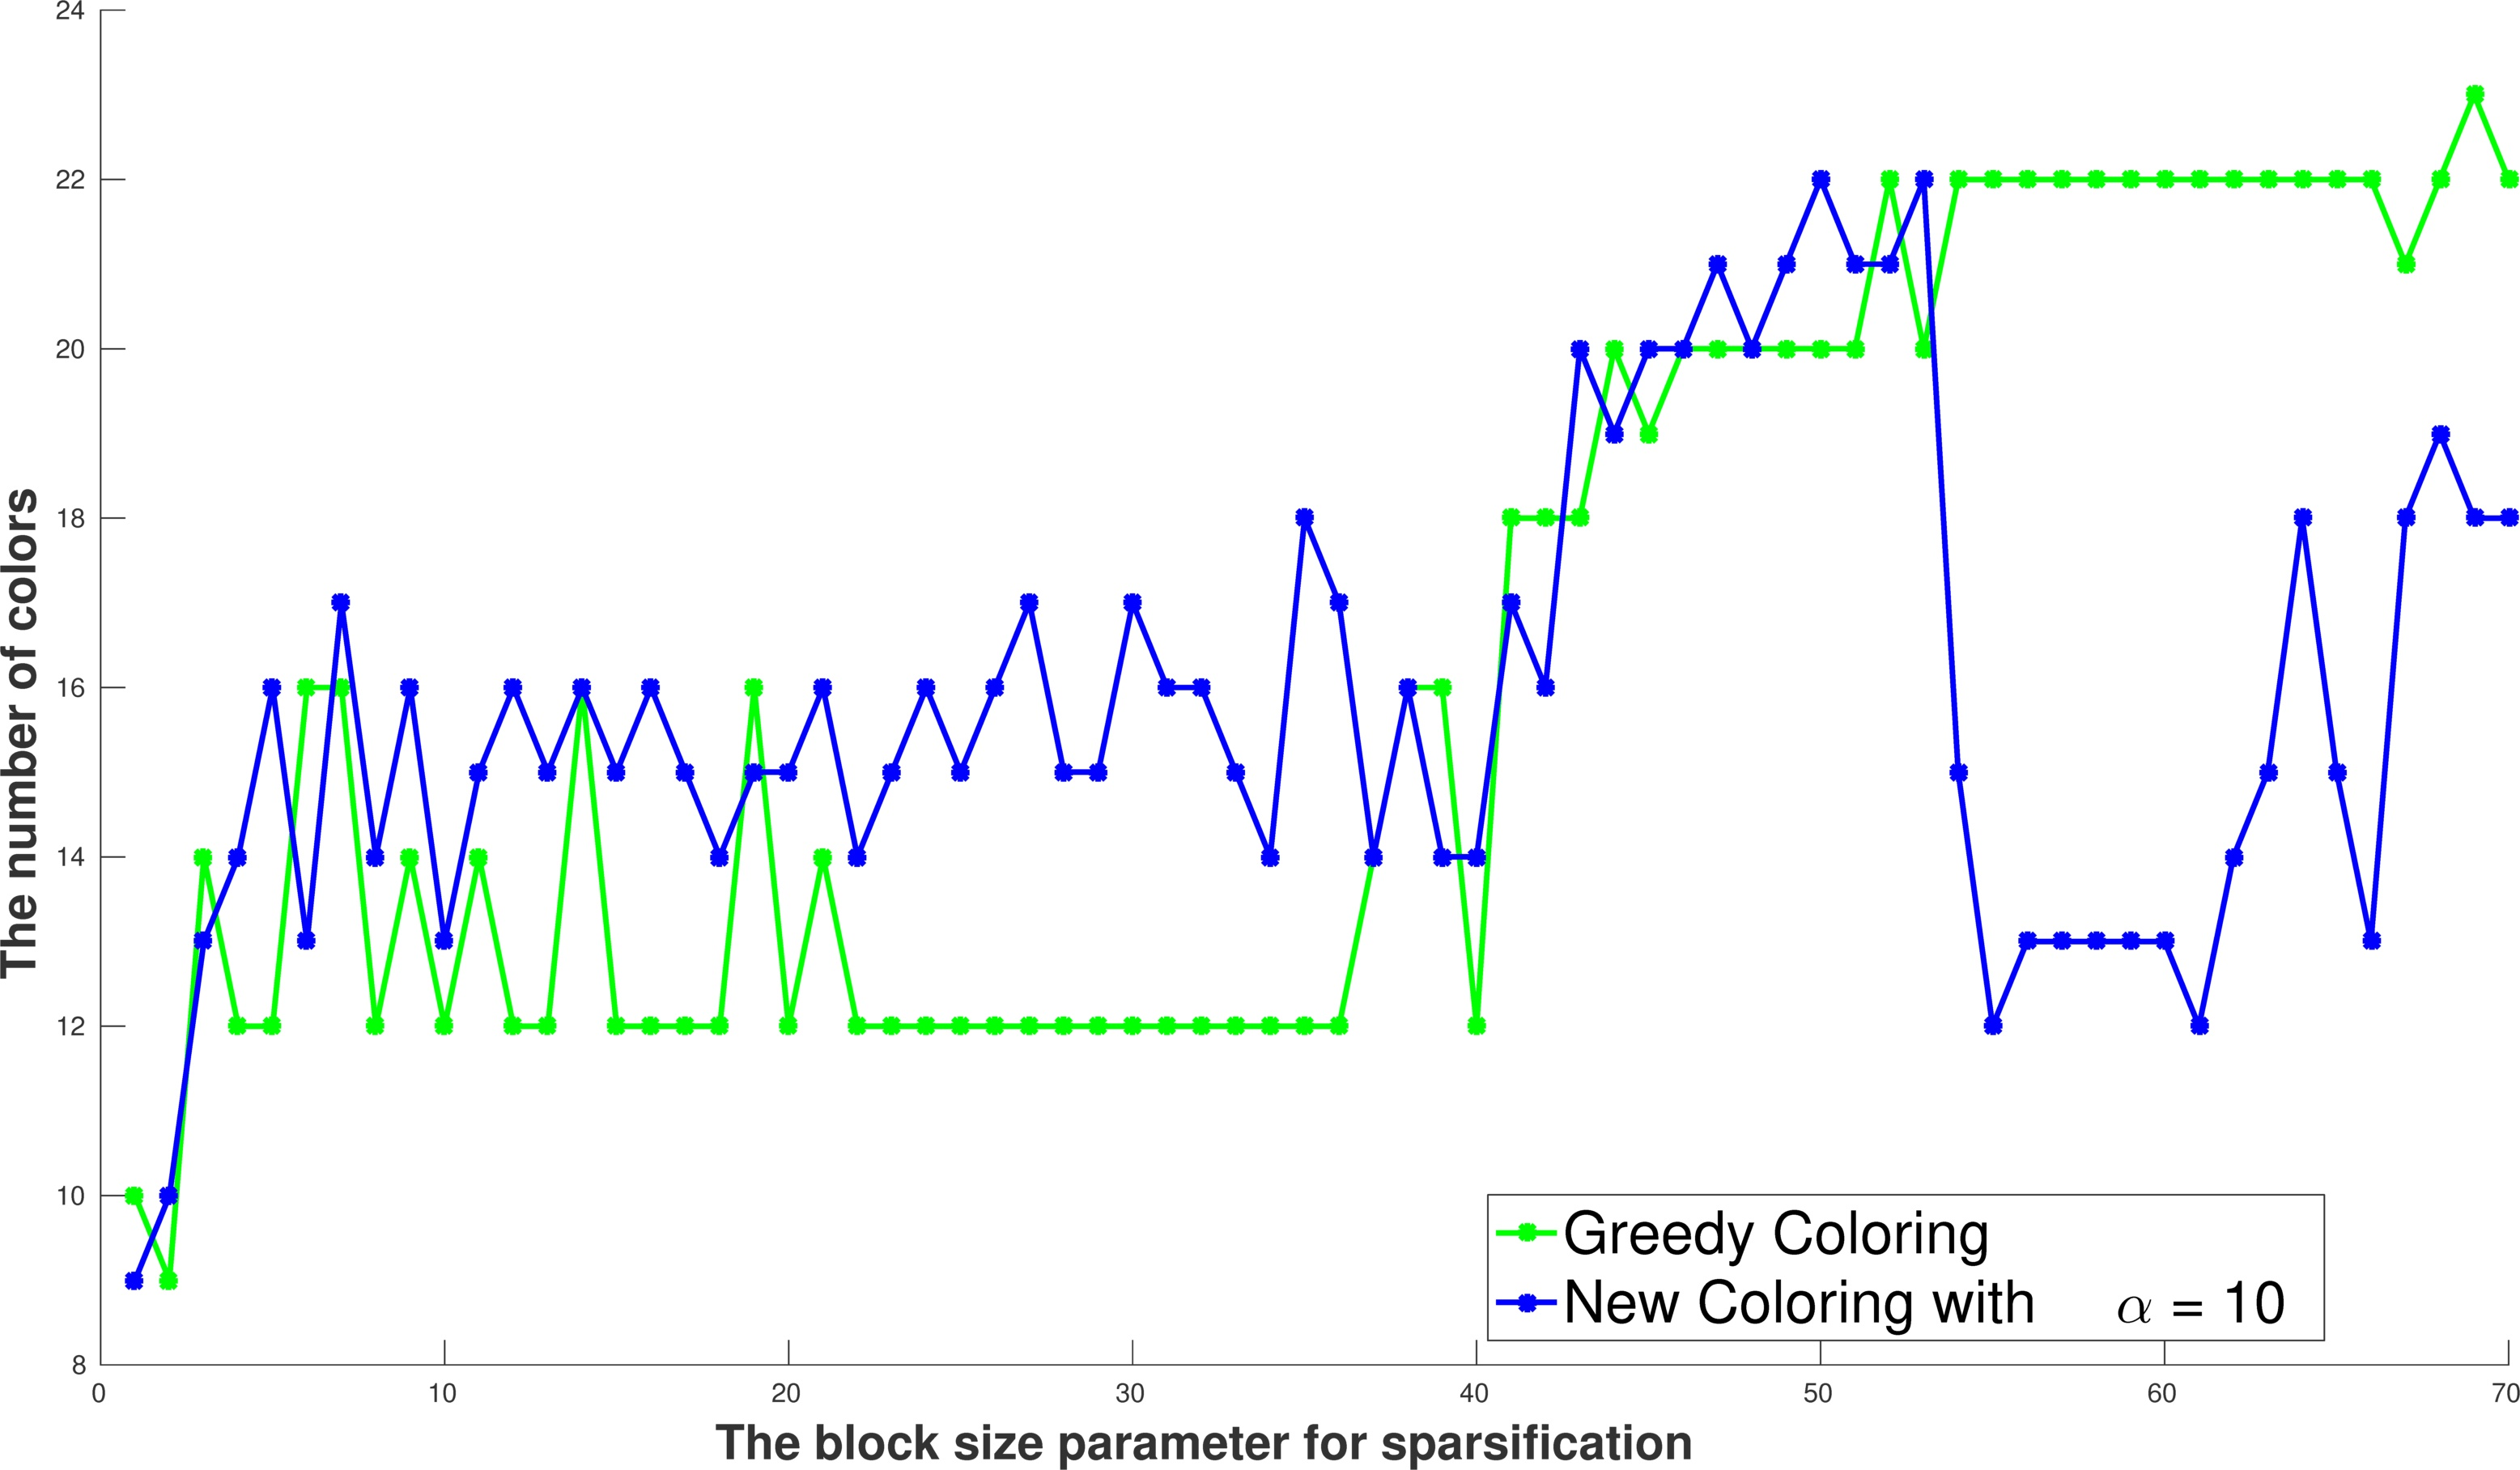
\includegraphics[width=0.9\linewidth]{bls_col_alpha_10_nos3}
\caption{The number of additionally required elements computed
by the new heuristics compared with the
greedy algorithm. The computation carried out on
the matrix \textit{nos3} and value of $\alpha$ is
set to $10$.}
\label{new.col.col.alpha.ten.nos3}
\end{figure}

\begin{figure}
\centering
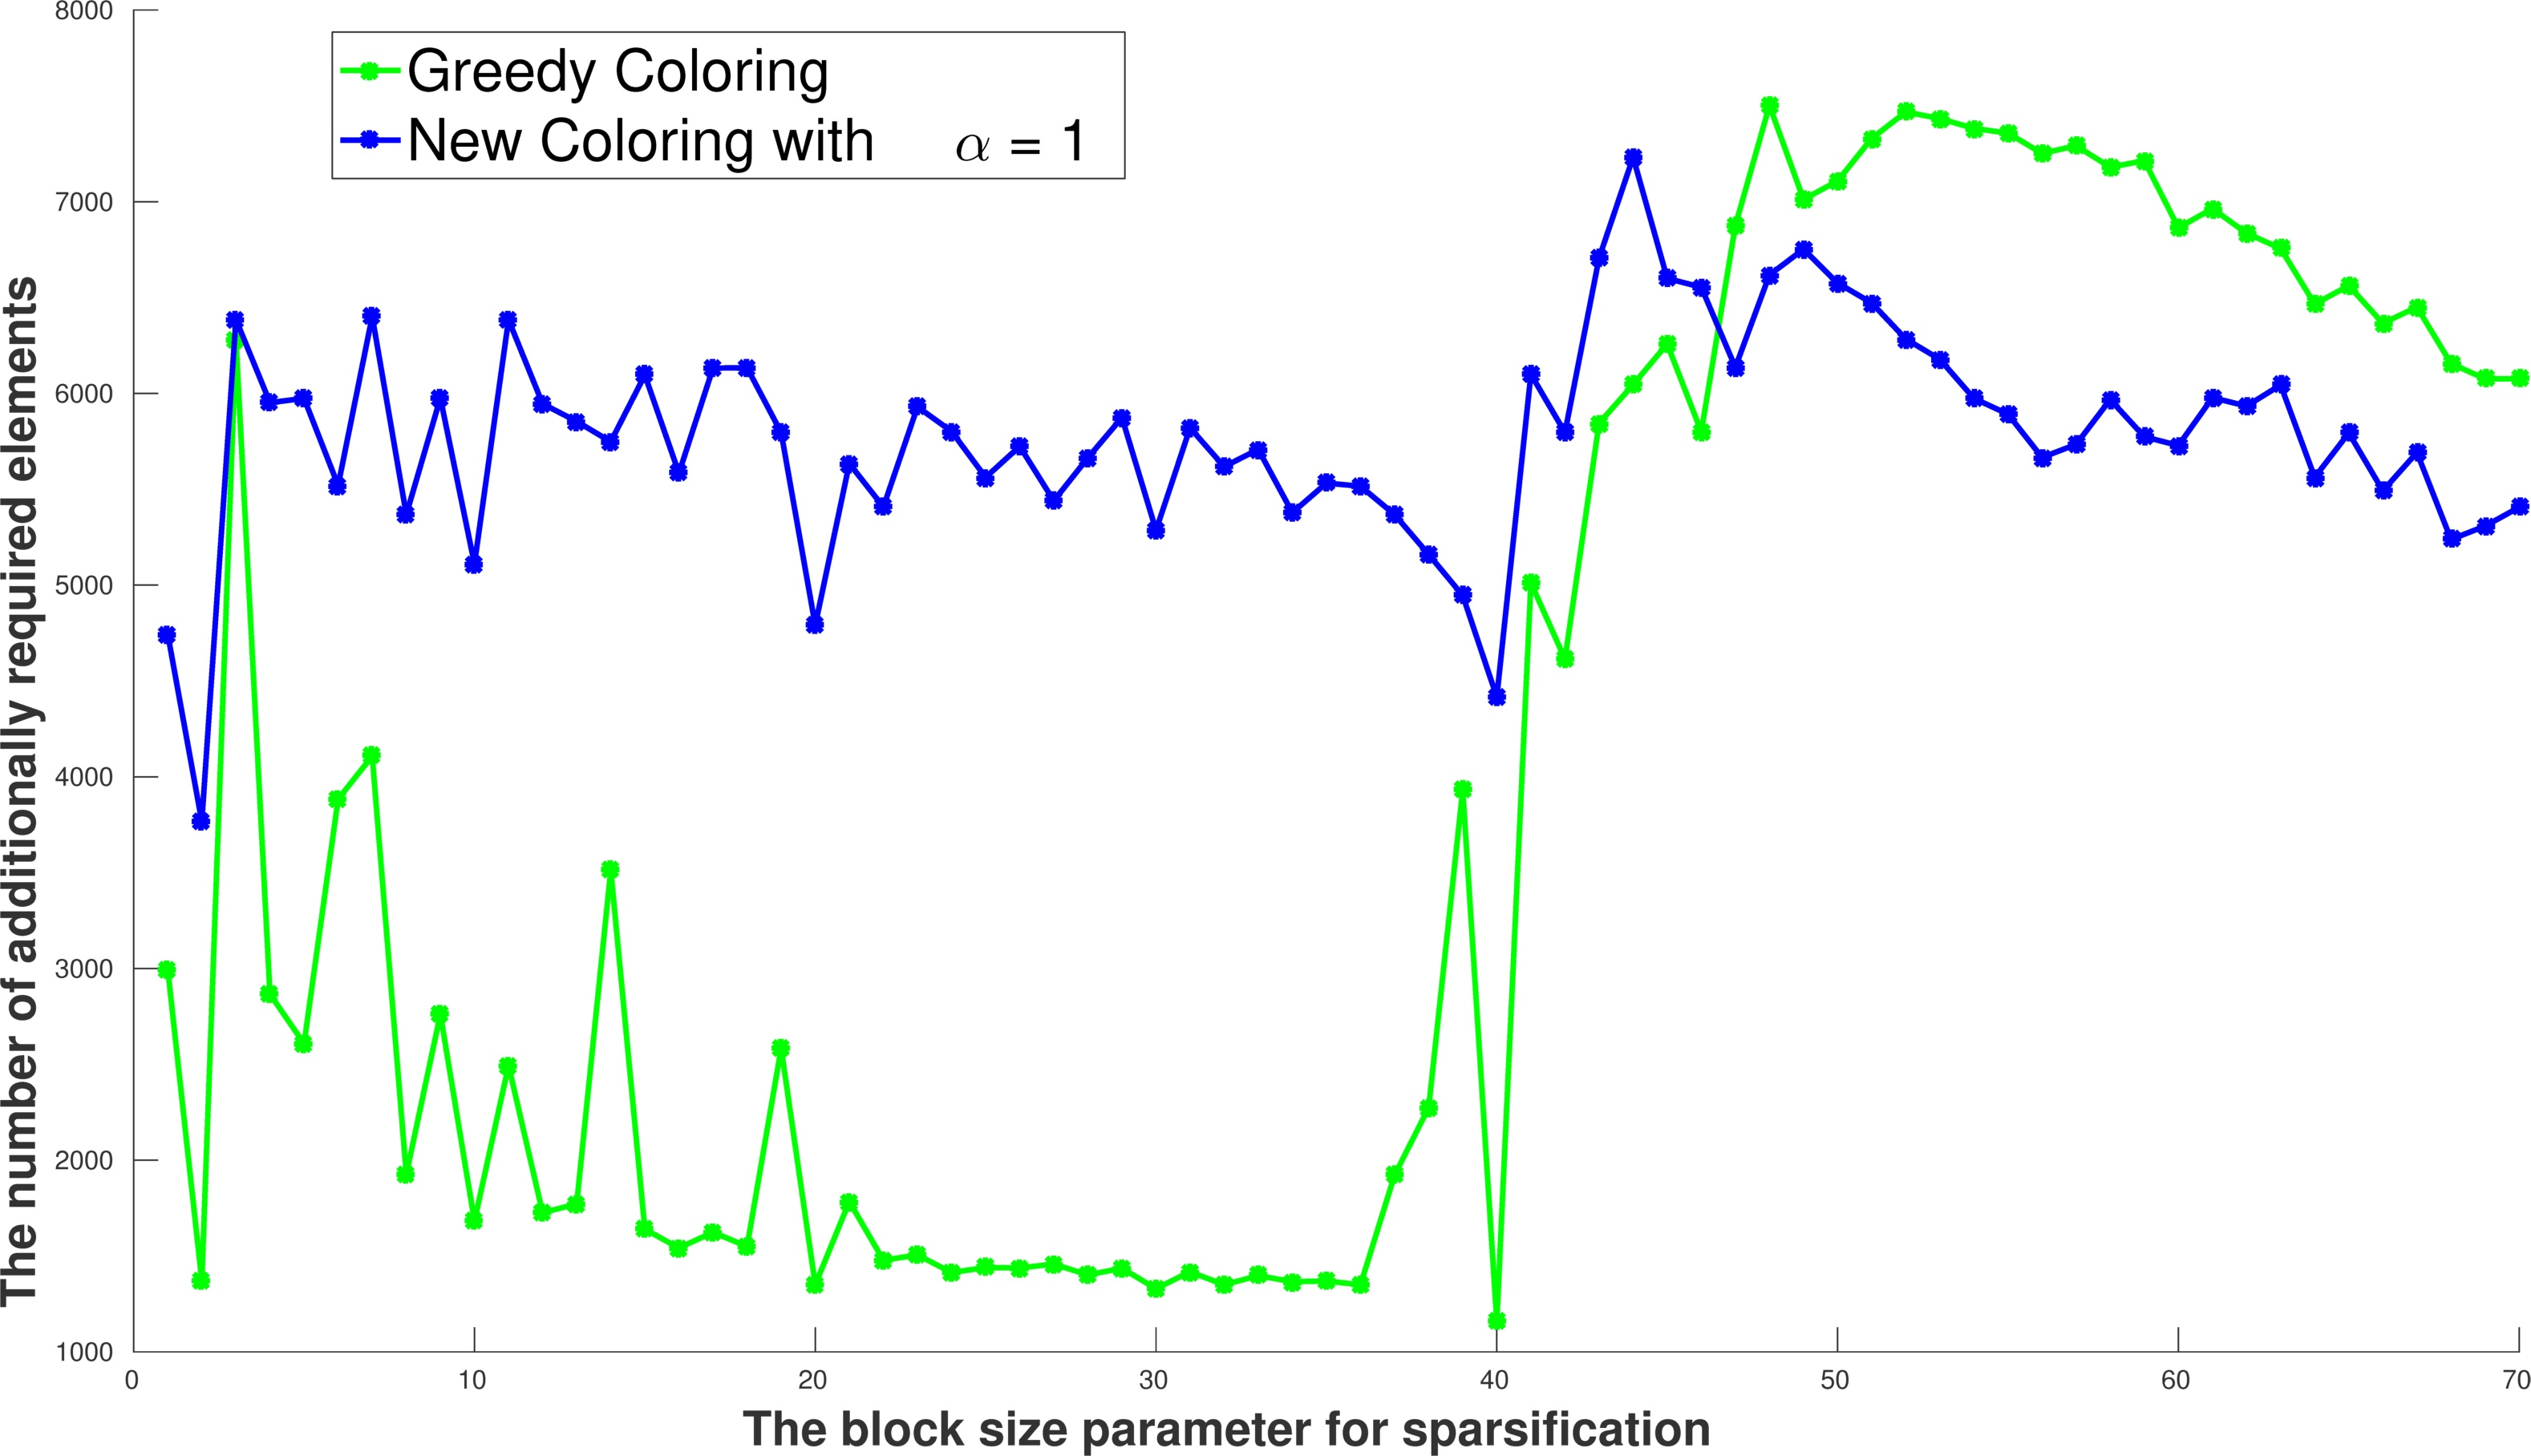
\includegraphics[width=0.9\linewidth]{bls_add_alpha_1_nos3}
\caption{The number of additionally required elements computed
by the new heuristics compared with the
greedy algorithm. The computation carried out on the matrix
\textit{nos3} and value of $\alpha$ is
set to $1$.}
\label{new.col.add.alpha.one.nos3}
\end{figure}
\begin{figure}
\centering
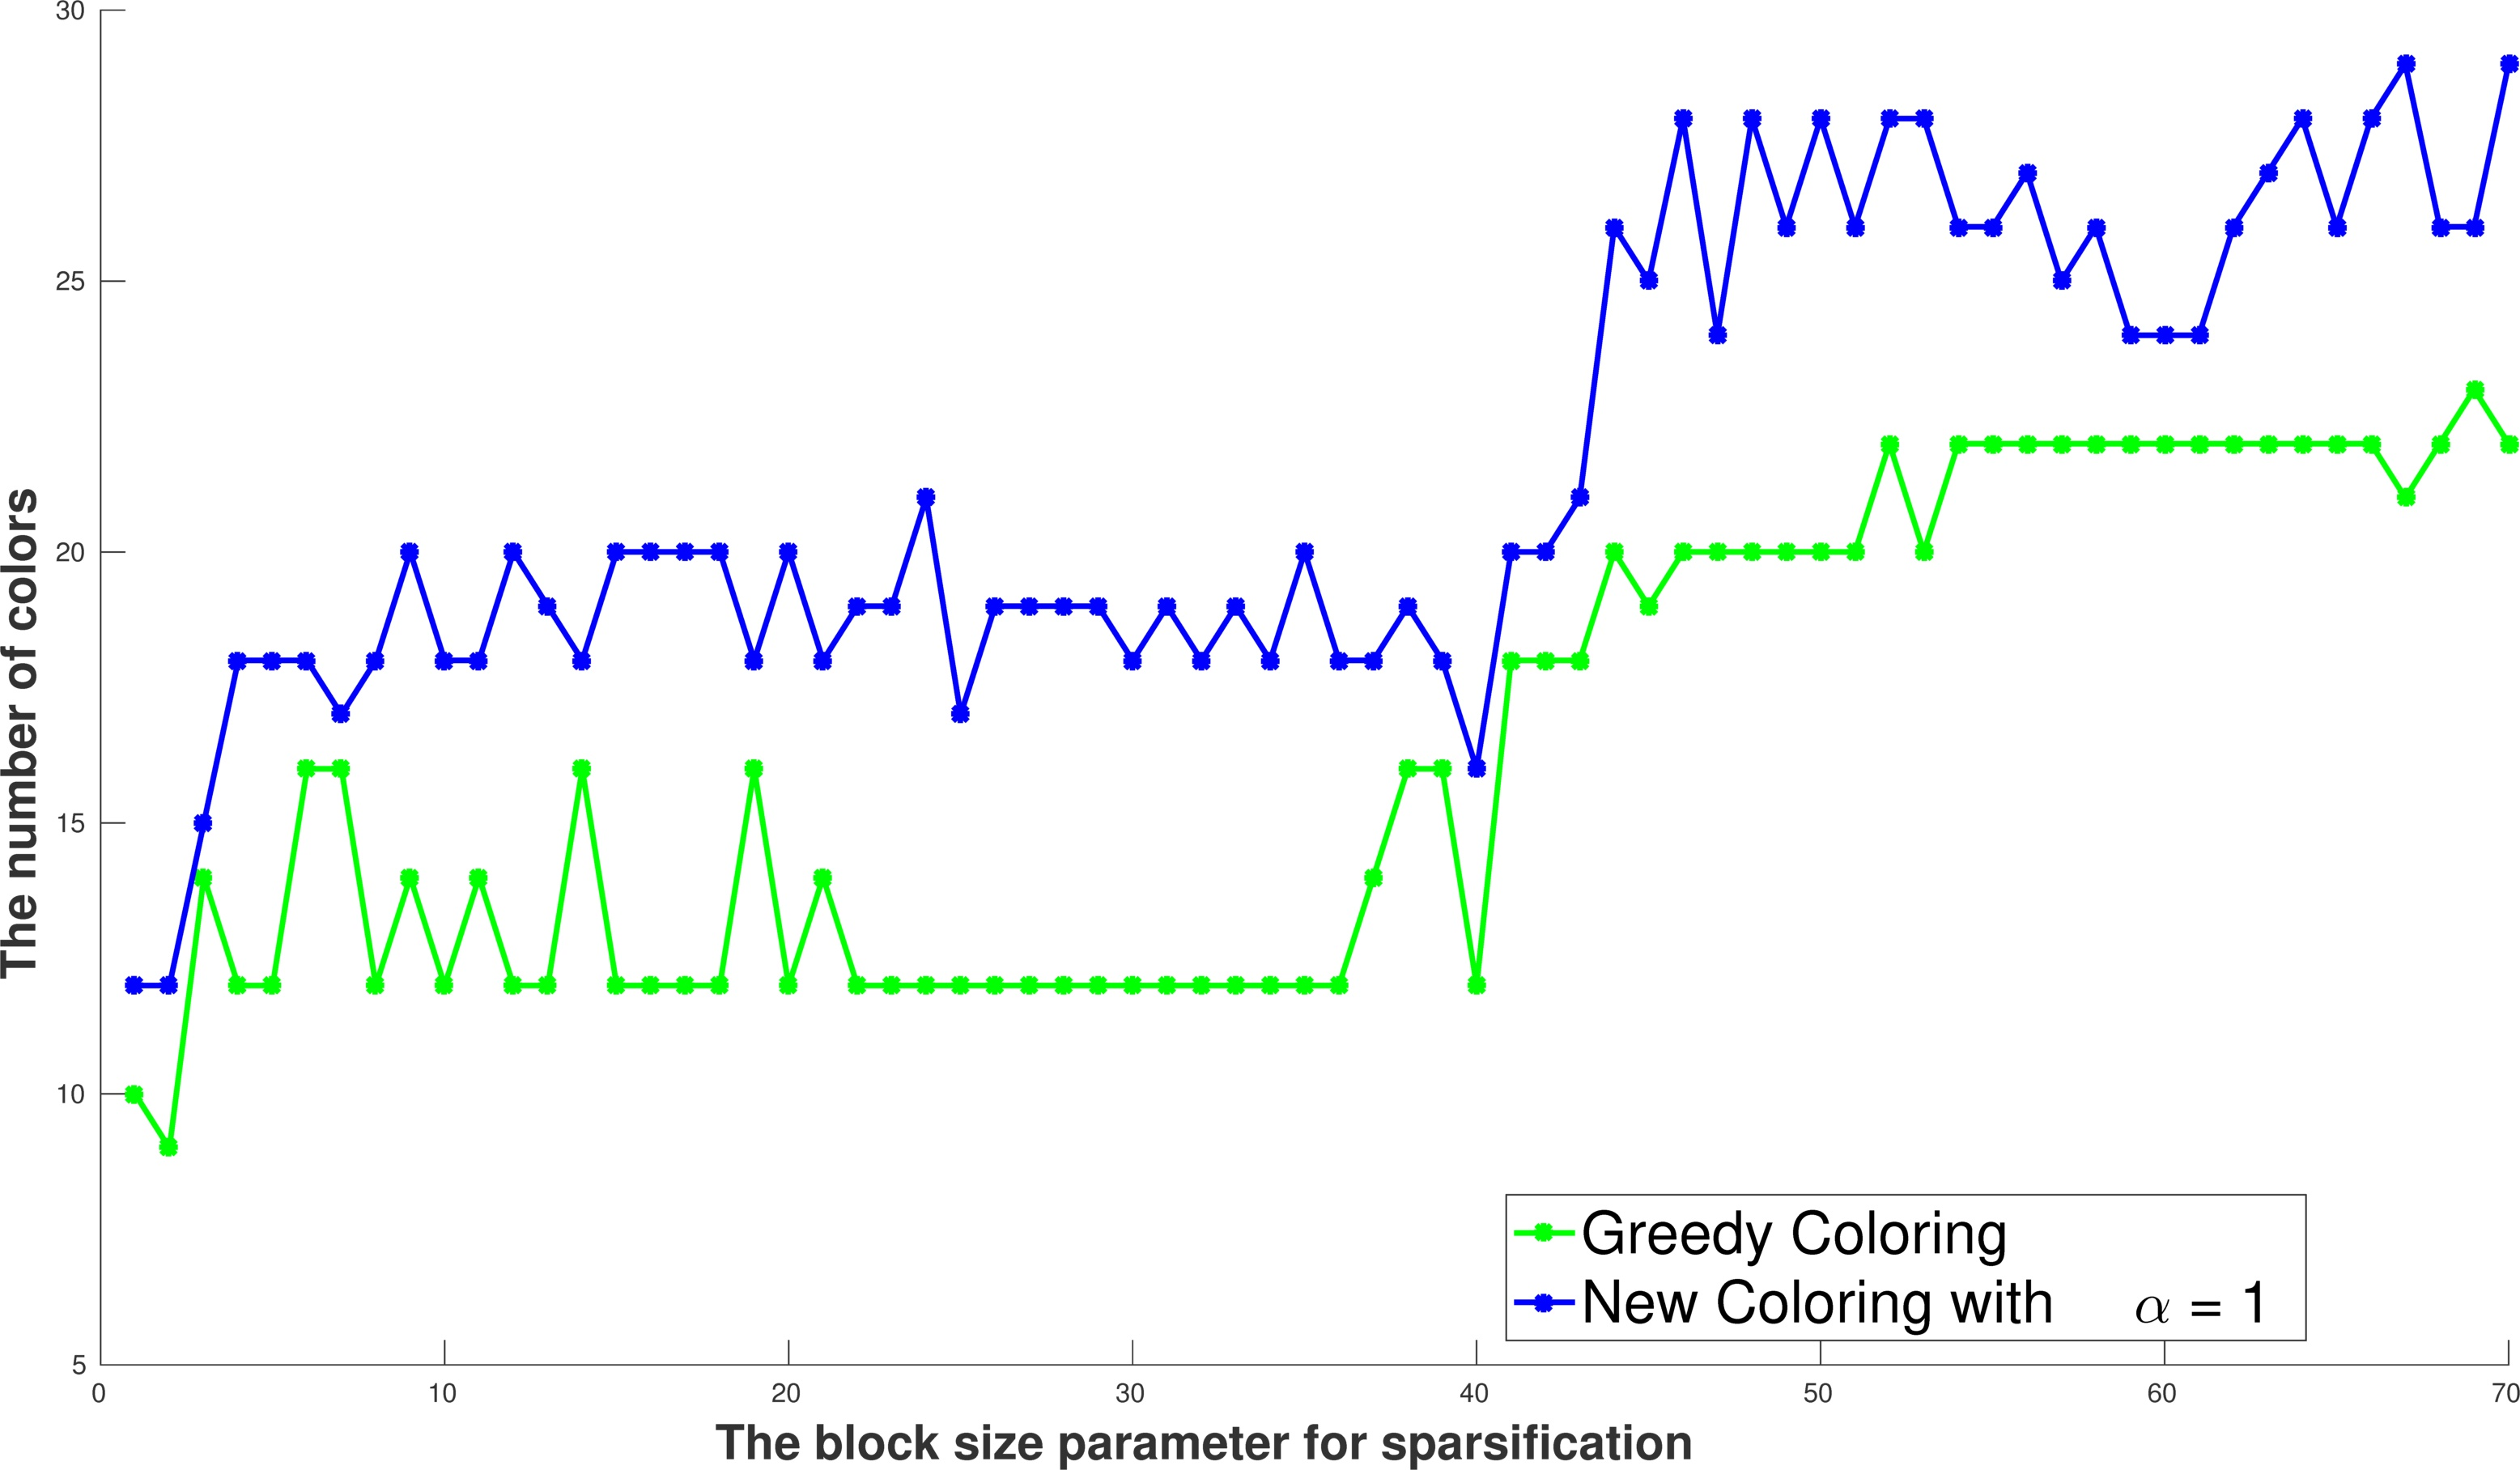
\includegraphics[width=0.9\linewidth]{bls_col_alpha_1_nos3}
\caption{The number of additionally required elements computed
by the new heuristics compared with the greedy algorithm.
The computation carried out on the matrix \textit{nos3}
and value of $\alpha$ is set to $1$.}
\label{new.col.col.alpha.one.nos3}
\end{figure}

\subsection{Star bicoloring}
\label{s.heuristic.starbicoloring}
The classical approach toward star bicoloring is first introduced in
\cite{Gebremedhin05whatcolor} as star bicoloring scheme.
This algorithm is implemented and evaluated in
Lülfesmann~\cite{LulfesmannMaster}. This algorithm performs convincing
since the steps of the algorithms is near to the definition of the coloring.
Complete direct solver bicoloring and Row/Column Fill Bicoloring~\cite{Hossain95computinga}
are the other algorithms which are introduced for bicoloring.
As Calotoiu~\cite{CalotoiuMaster} dicusses theses algorithms do not perform
better than the classic star bicoloring scheme.
Calotoiu~\cite{CalotoiuMaster} introduces the integrated star bicoloring
and total ordering star bicoloring which performs better than
star bicoloring scheme in some matrices and not much worse in some other
matrices.

As same as the last section, we search for a modified version of star bicoloring
which increases the number of additionally required elements without
a high increase the number of colors. The idea from the new heuristic
can be applied here. However it can survive less additionally required
elements since a survived nonrequired elements from the column compression
it is not necessary a survived nonrequired elemtns form the row compression.

We consider the implemenetation of star bicoloring in \coderef{orig.star.bicoloring} based on
the algorithm from Lülfesmann~\cite{Lulfesmann2012Fap}.
Here, the notation $G[S]$ means the graph induces on the edge set $S$.
\begin{figure}
\begin{lstlisting}[
caption=A new heuristic for star bicoloring algorithm
considering the survived nonrequired elements.,
label=orig.star.bicoloring,mathescape]
function star_bicolor_nreq($G=(V_r\cup V_c,E)$,$E_i\subset E$)
for $v\in V_c$
  $\Phi(v)=-1$
  $forbiddenColors[v] = 0$

$v = -1$
$E_R^{'} = E_R$
while $E_R^{'}$ is not empty
  if($\Delta(V_r,G[E_R^{'}]) > \rho \Delta(V_c,G[E_R^{'}])$ then
    v = $v_r\in V_r$ with maximum degree in $G[E_R^{-1}]$
  else
    v = $v_c\in V_c$ with maximum degree in $G[E_R^{-1}]$
  $E_R^{'} = E_R^{'} - {(v,w)\in E_R^{'}:w\in N_1(v,G[E_R^{'}])}$
  for all $w\in N_1(v,G)$
    if $\Phi(w) \leq 0$
  for all $x\in N_1(w,G)$ with $\Phi(w) > 0$
    if $(v,w) \in E_R$ or $(w,x) \in E_R$
      $forbiddenColors[\Phi (x)]=v$
    else
      for all $x\in N_1(w,G[E_R])$ with $\Phi(w) > 0$
      for all $y\in N_1(x,G)$ with $\Phi(y) > 0$ and $y\neq w$
        if $\Phi(w) = \Phi(y)$
          $forbiddenColors[\Phi (x)] = v$
          $\Phi(v) = min(\{j>0: forbiddenColors[j] \neq v\})$
          for all $v_c\in V_c$ with $\Phi(v_c) > 0$
            $\Phi (v_c) = \Phi (v_c) + max(\{\Phi (v_r): v_r \in V_r\})$
          for all $v\in V_r\cup V_c$ with $\Phi(v)\neq -1$
            $\Phi (v) = 0$
\end{lstlisting}
\end{figure}
This algorithm process a vertex either from column vertices
or row vertices with maximum degree in each step.
We first did some computations to find the influence of $\rho$ on the
number of additioanlly required elements. The value of $\rho$ is a weightening factor which
is a balance between columns or row vertices. A higher value of $\rho$
makes the compression mostly in the column vertices and vice versa.
There are some discussion on how to choose the value of $\rho$ in
\cite{Gebremedhin05whatcolor}. Also,
Lülfesmann~\cite{Lulfesmann2012Fap,LulfesmannMaster} did som computation for some
specific $\rho$.
However, the main goal in these previous literature
is to minimize the number of colors.
As the \figref{rho_value_685_bus} and \figref{rho_value_orani678},
the value of $\rho$ has definitely a direct influence on
the number of additionally required elements.
The interesting observation is that a tiny change
on the value of $\rho$ can dramatically change the
results. For example, changing the value of $\rho$ from
$0.3$ to $0.4$ in \figref{rho_value_orani678} would result
in a change of $10000$ in the number of additionally required elements.

\begin{figure}
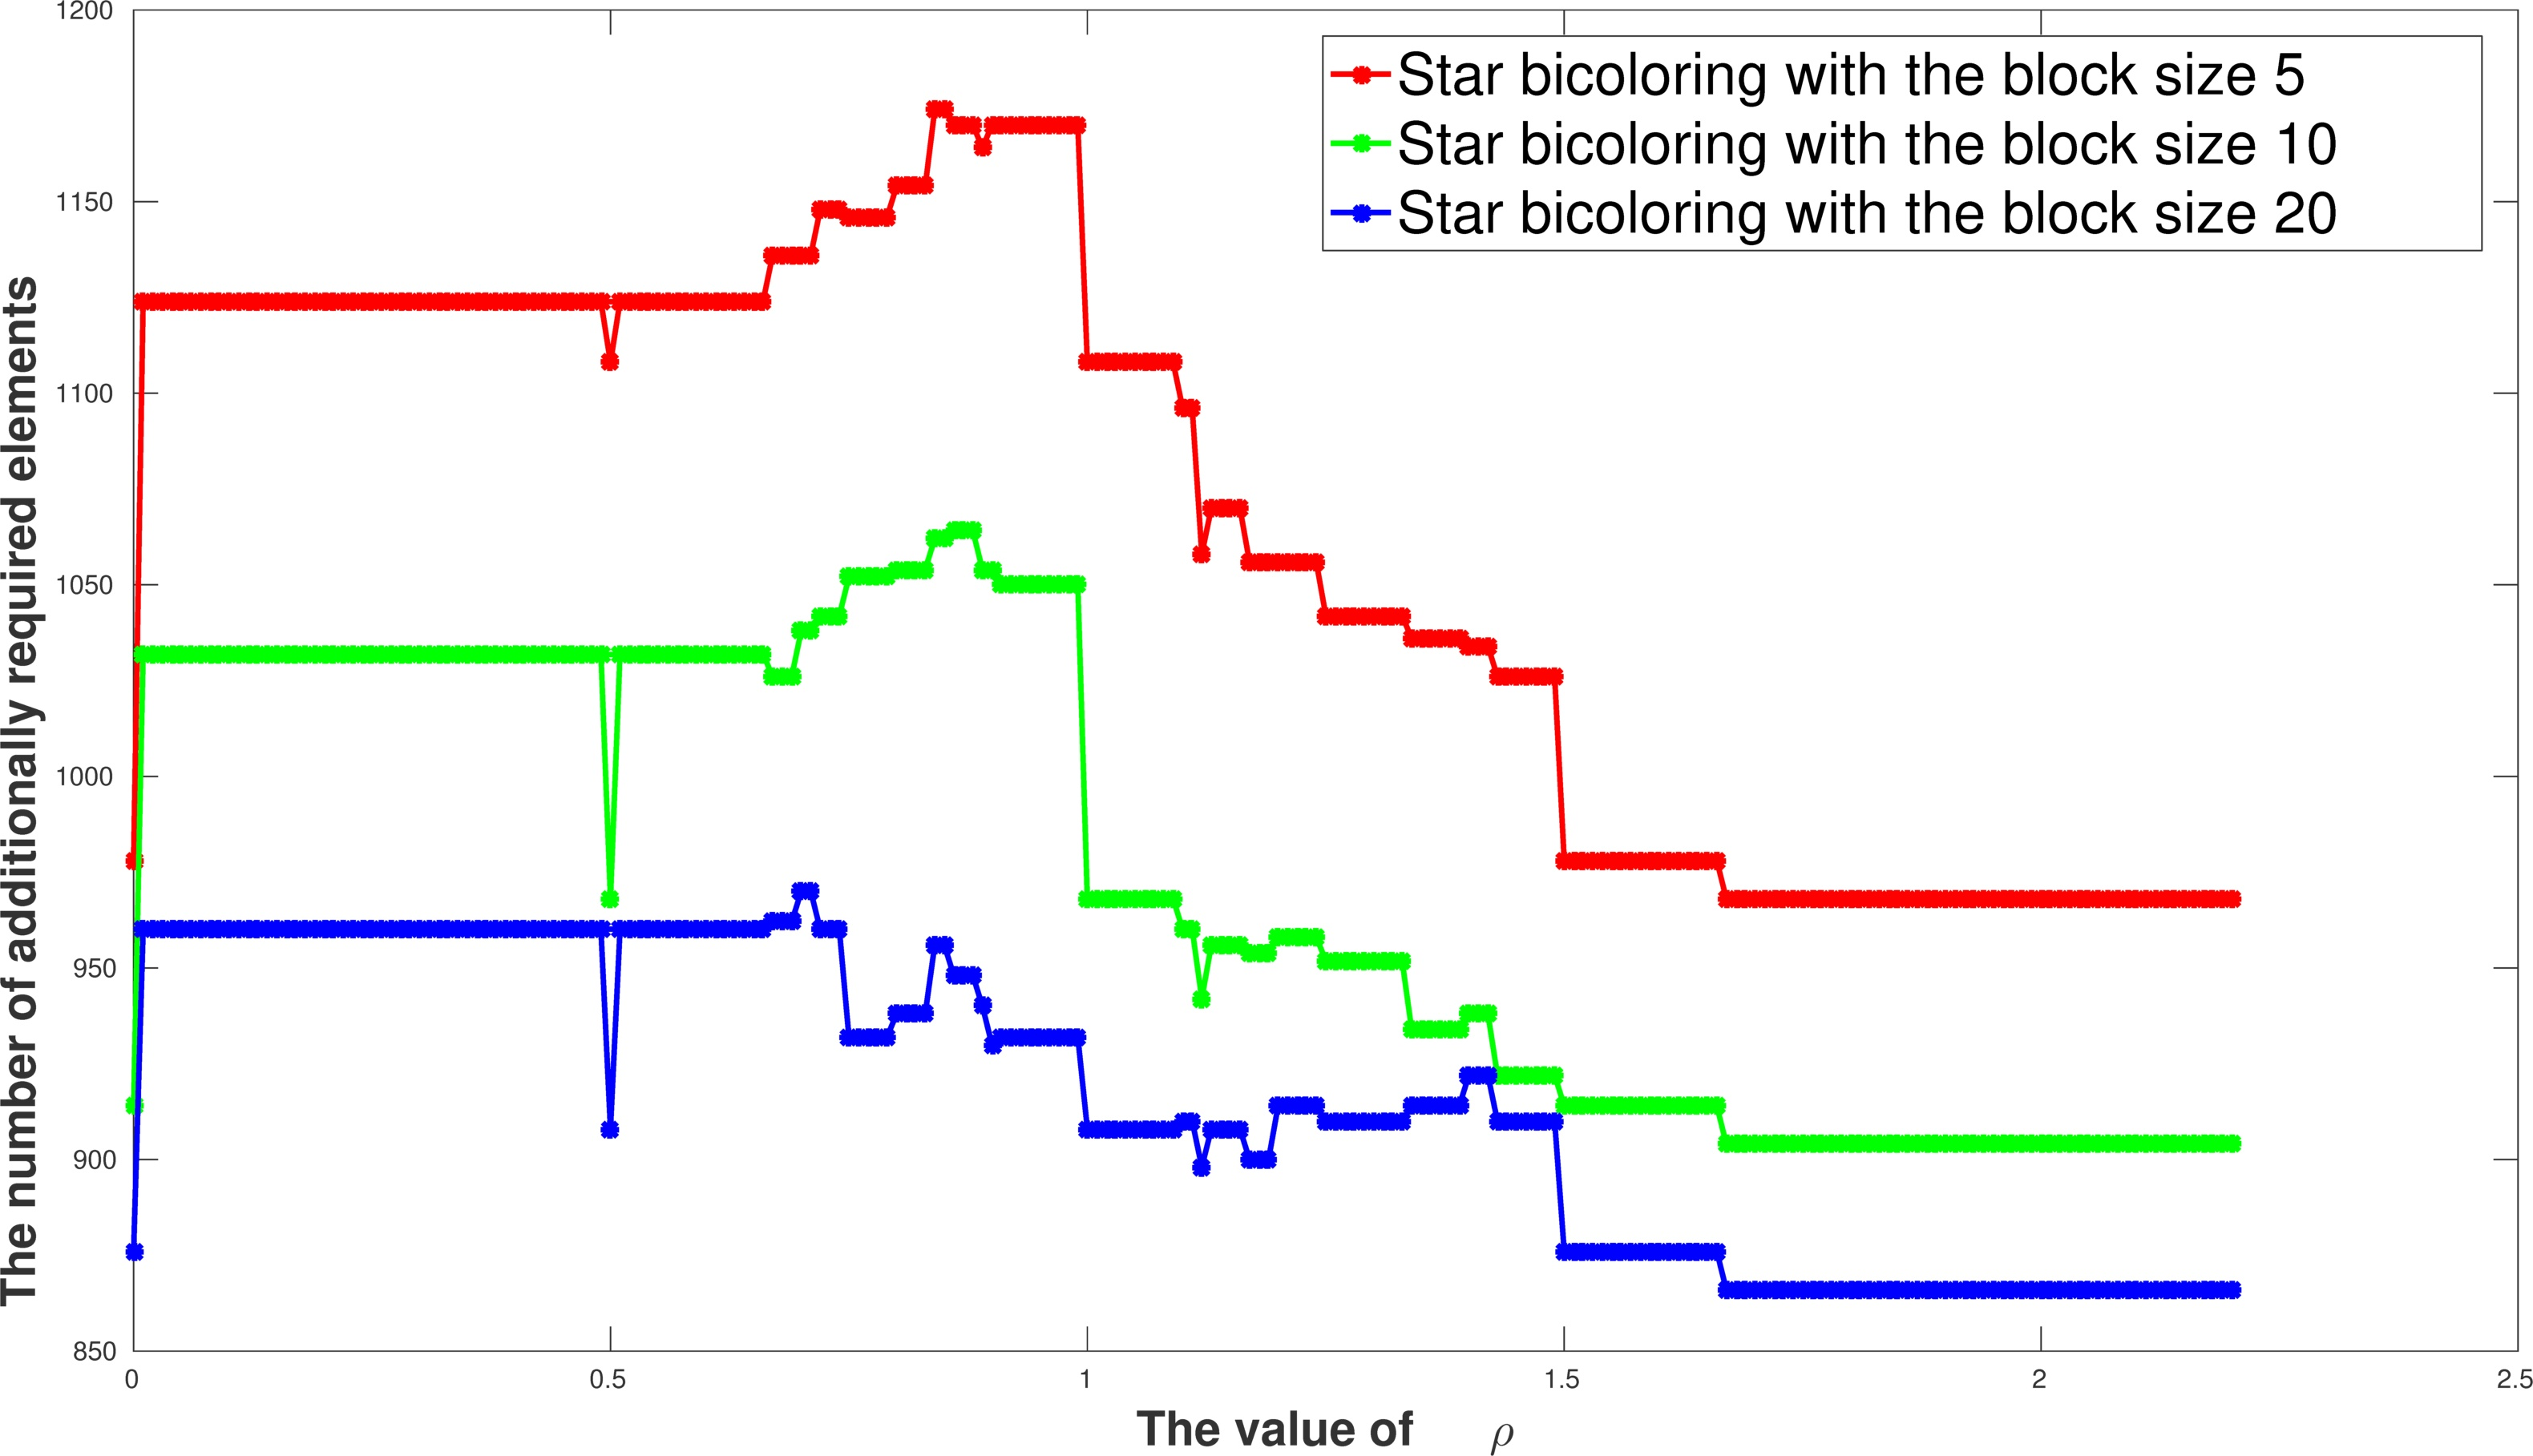
\includegraphics[width=0.9\linewidth]{rho_value_685_bus}
\caption{The influence of $\rho$ is computed on the additionally required elements
for the matrix \textit{685\_bus}.}
\label{rho_value_685_bus}
\end{figure}

\begin{figure}
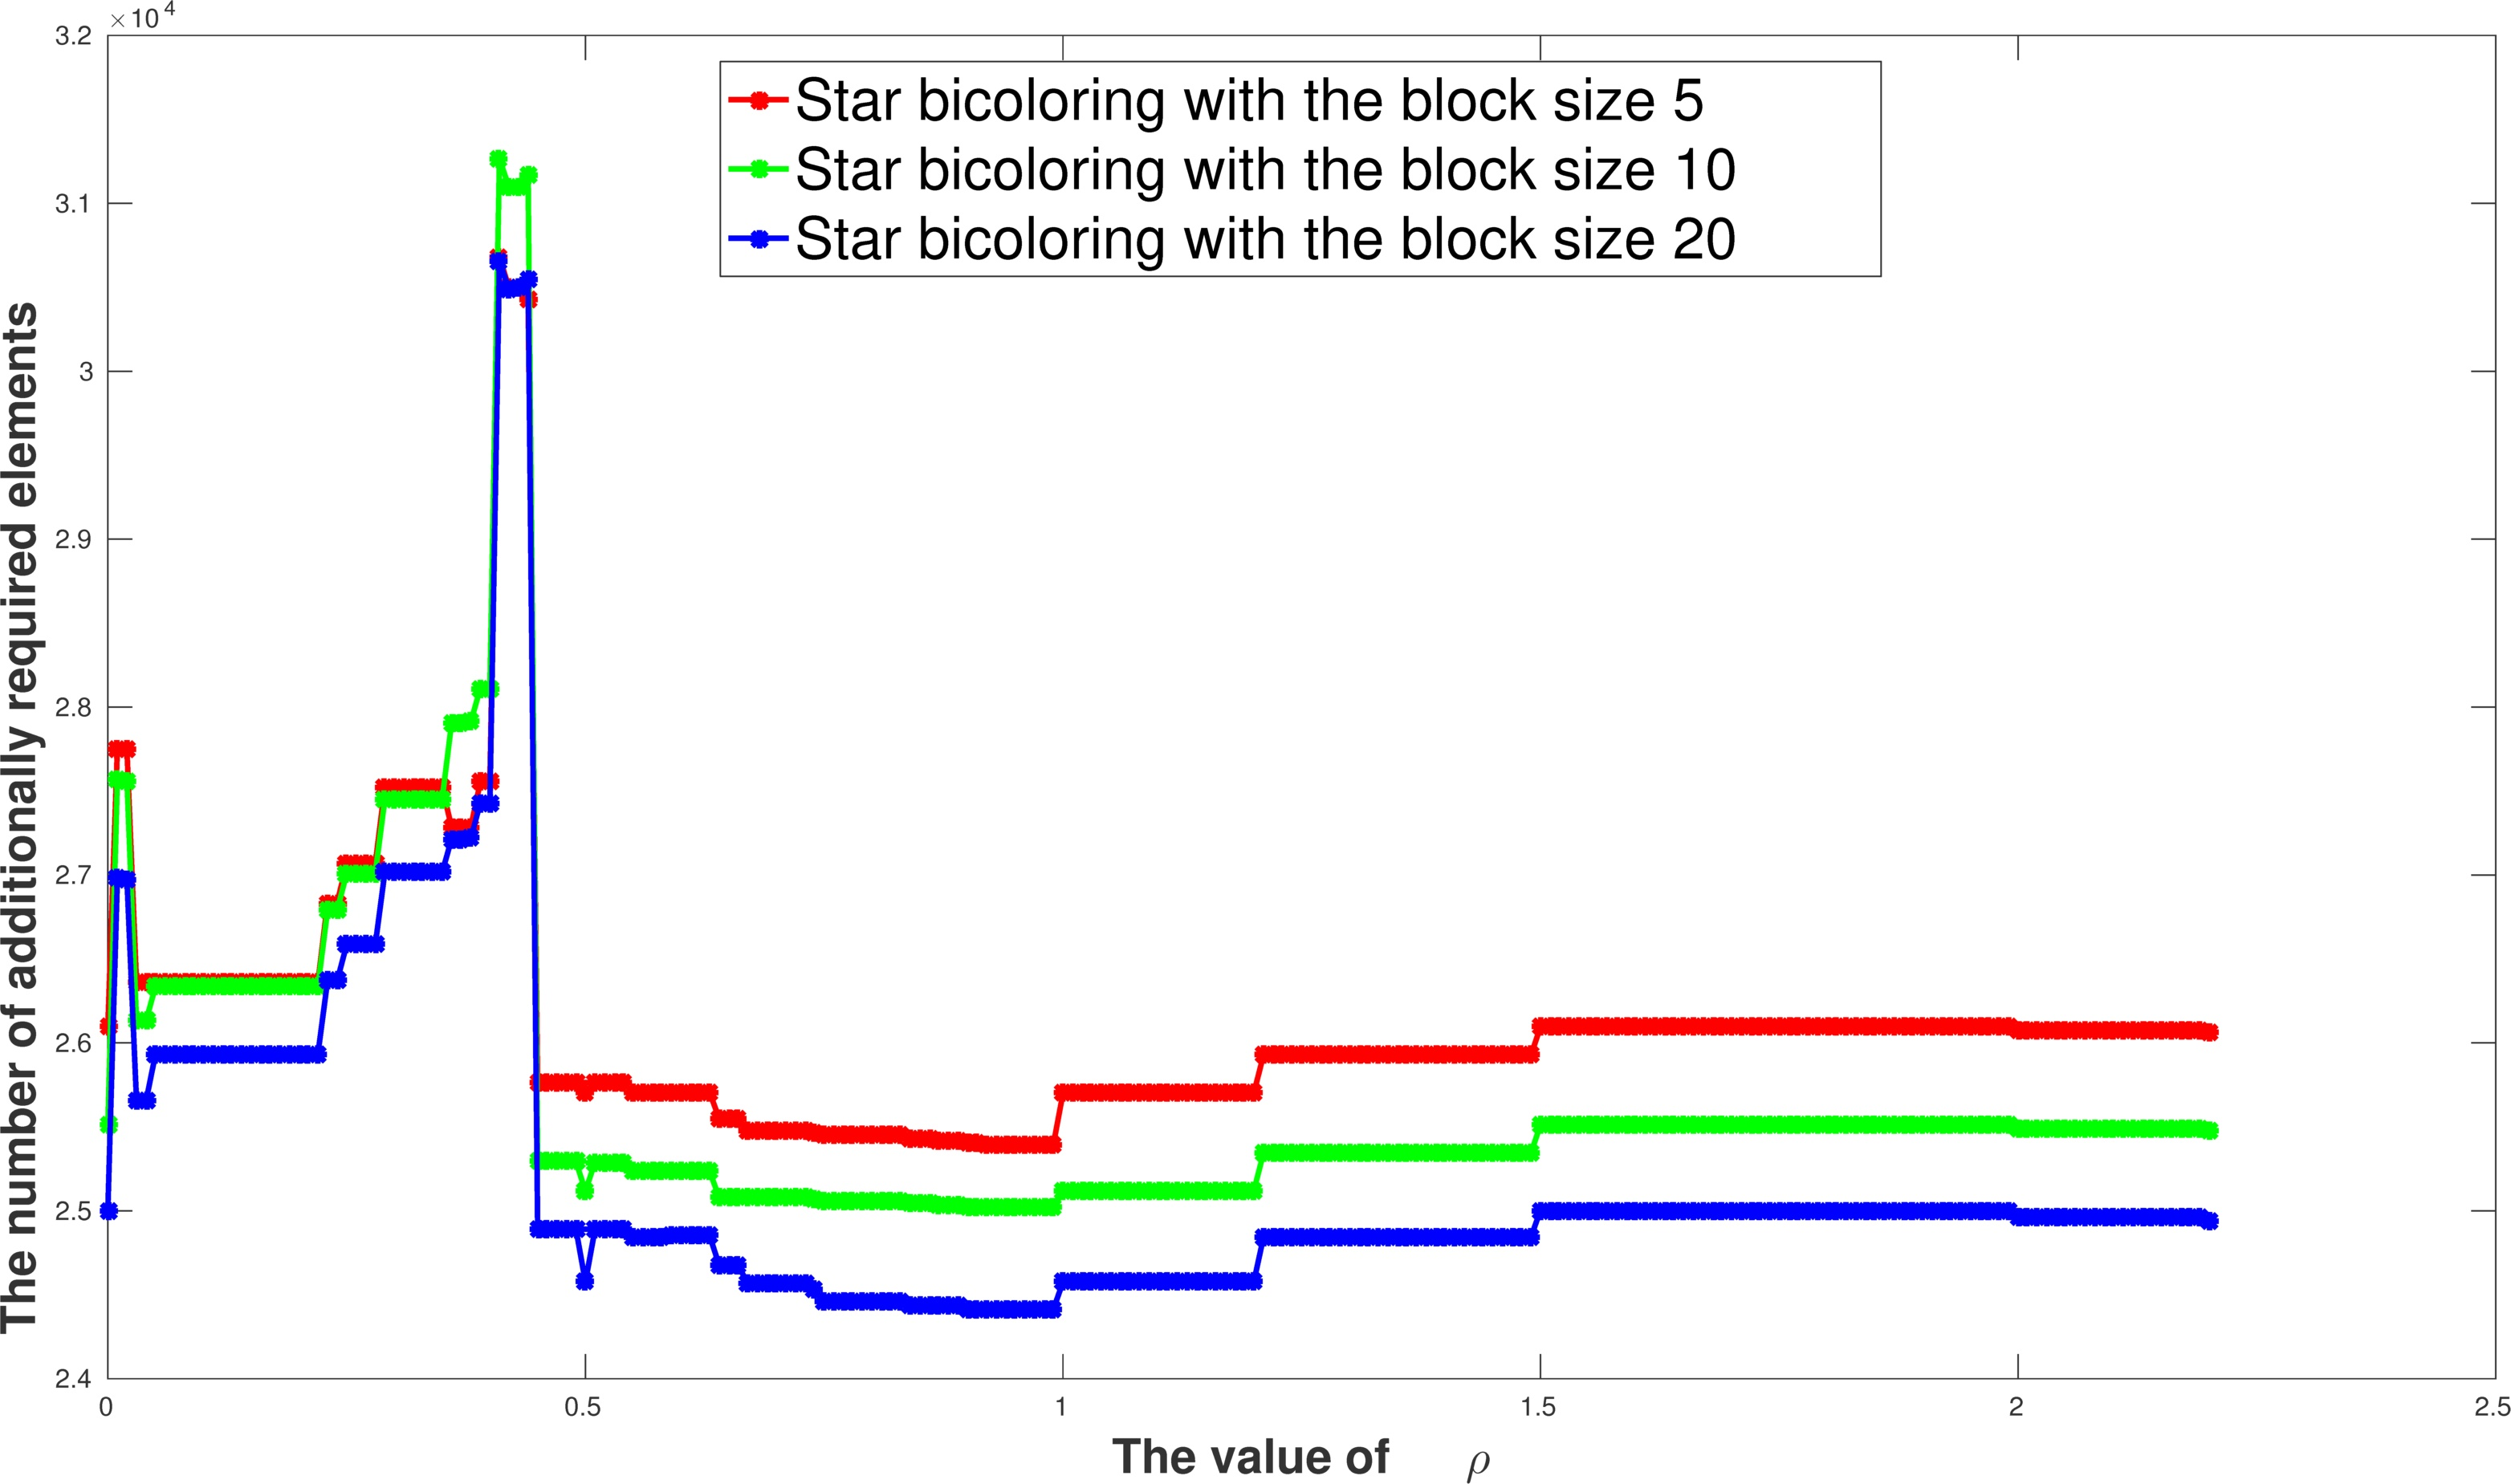
\includegraphics[width=0.9\linewidth]{rho_value_orani678}
\caption{The influence of $\rho$ is computed on the additionally required elements
for the matrix \textit{orani678}.}
\label{rho_value_orani678}
\end{figure}

As we said, the first part of algorithms chooses the next vertex
which should be processed from the maximum degree vertices
in a graph induces on the required edges.
We change this part of algorithm to process a specific algorithm
with maximum degree and maximum nonrequired elements instead of
an arbitrary vertex. After the first step, this processes can be
repeated or we can process the vertices with
minimum number of nonrequired elements.

\begin{figure}
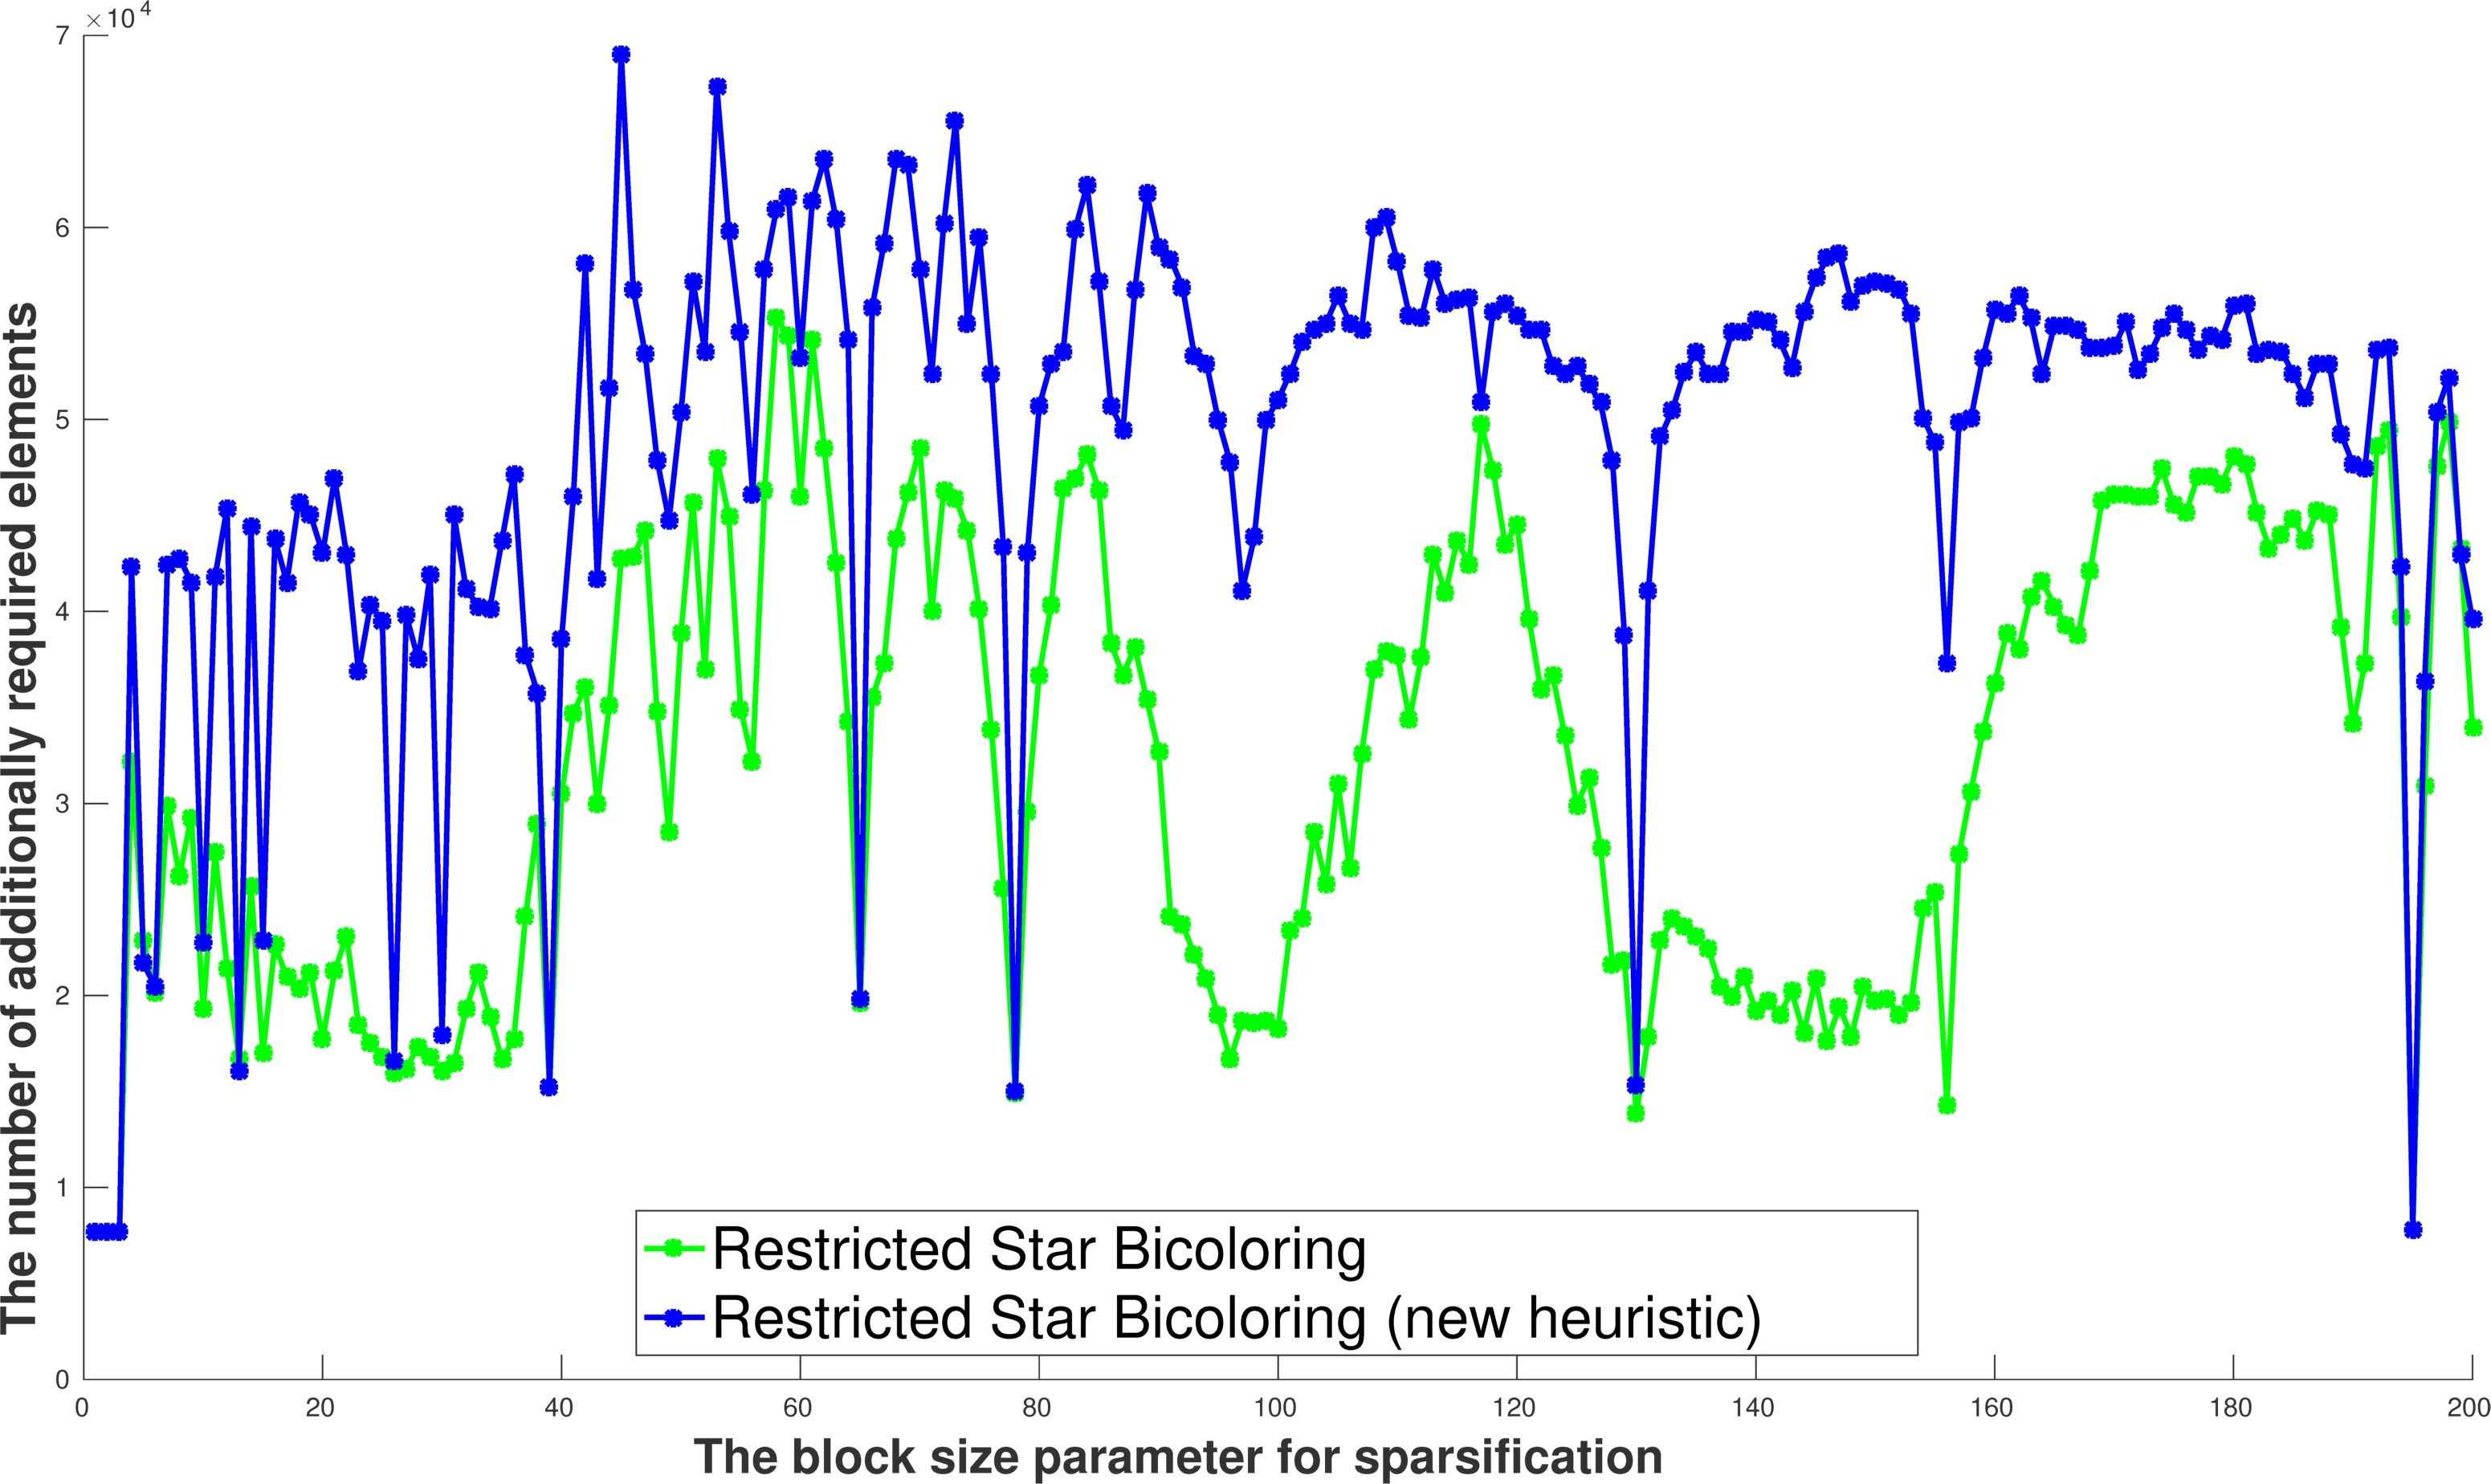
\includegraphics[width=\linewidth]{bls_adds_crystm01_old_star_vs_new}
\caption{The number of additionally required elements computed with
the new star bicoloring compared with the older implementation.
The asymmetric matrix \textit{$crystm01$} is used here.}
\label{bls_adds_crystm01_old_star_vs_new}
\end{figure}

\begin{figure}
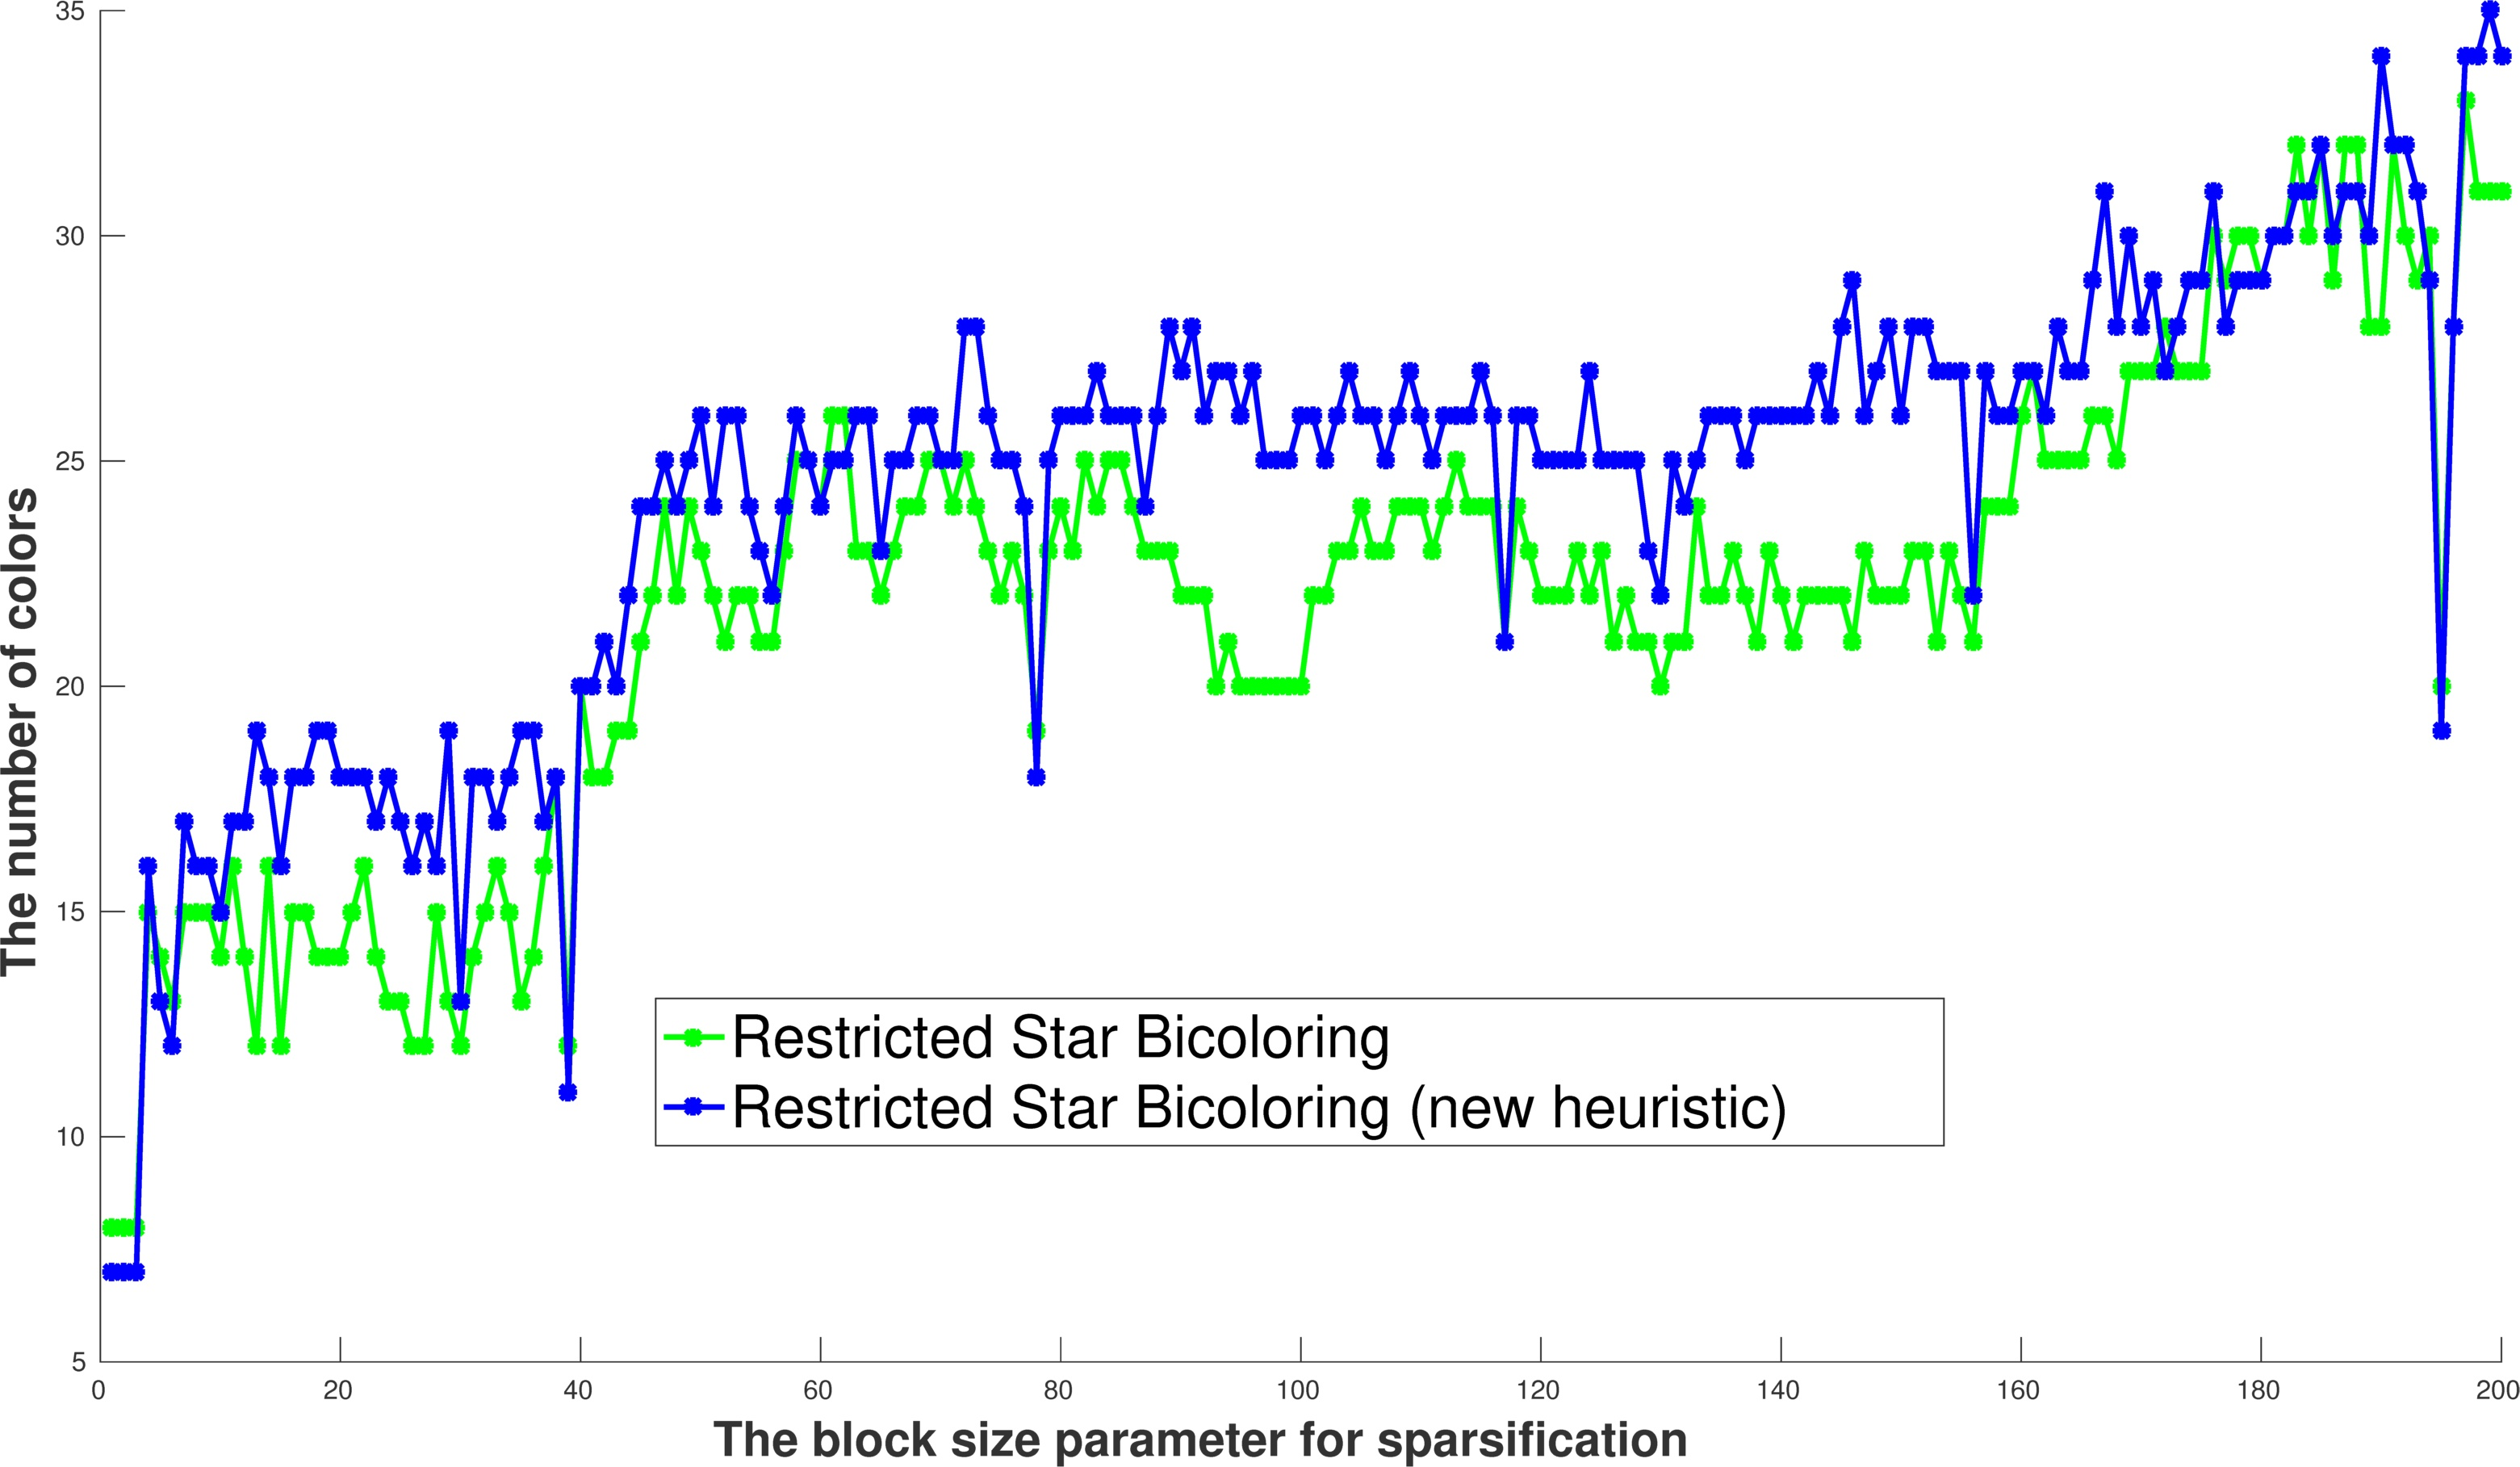
\includegraphics[width=\linewidth]{bls_cols_crystm01_old_star_vs_new}
\caption{The number of additionally required elements computed with
the new star bicoloring compared with the older implementation.
The asymmetric matrix \textit{$crystm01$} is used here.}
\label{bls_cols_crystm01_old_star_vs_new}
\end{figure}
%%%%%%%%%%%%%%%%%%%%%%%%%%%%%%%%%%%%%%%%%%%%%%%%%%%%%%%%%%%%%%%%%%%%%%%%%%%%%%%%%%%%%%%%
\section{Maximizing Additionally Required Elements}
\label{s.max.add.req}
%%%%%%%%%%%%%%%%%%%%%%%%%%%%%%%%%%%%%%%%%%%%%%%%%%%%%%%%%%%%%%%%%%%%%%%%%%%%%%%%%%%%%%%%%
In \secref{s.heuristic}, our focus was to increase the potentially required elements
which probably increases also the number of the additionally required elements.
Here, we check directly in the process of coloring
if a potential required element can be an additionally required elements.
For this purpose, we use the bipartite graph model for ILU preconditioning
as well as the fill path theorem introduced
in~\secref{ss.comb.precond} to be consistent with the bipartite graph model for coloring.

In \coderef{code.new.impr1}, we compute the required nonzero elements
The idea is to check if the current nonzero required elements

\subsection{Experiments on Effects of Orderings}
\label{s.ilu}
In the idea of mixing the preconditioning and AD discussed in~\secref{s.precond},
the ILU preconditioning is computed using the natural ordering of the given matrix. However,
it is a well-known fact that the number of fill-ins is highly dependent on the ordering.
So, we can improve the number of fill-ins by carefully choosing an ordering.
On the other hand, we compute the Jacobian matrix by AD techniques in which
the matrix computed in a specific ordering. We need a reformulation to
fit these two computations from ILU preconditioning and the automatic differentiation.

As we discussed in the iterative solvers, like BICGSTAB,
we always need to have a matrix-vector product like $Az$.
This suits the AD behavior which gets a seed matrix, here the vector $z$, and
computes the matrix-vector product.
A reordering of the matrix for ILU preconditioning
needs a consideration also in the seed matrix.
Without reordering, a preconditioning would look like as,
$$
Ax = b \rightarrow M^{-1} Ax = M^{-1}b.
$$
We would add the reordering to this equation results in the following equations,
\begin{align*}
Ax = b \rightarrow M^{-1} Ax &= M^{-1}b\\
P^T M^{-1} P P^T A P P^T x &= P^T M^{-1} P P^T b\\
(P^T M^{-1} P) (P^T A P) P^T x &= (P^T M^{-1} P) P^T b\\
(P^T M P)^{-1} (P^T A P) P^T x &= (P^T M P)^{-1} P^T b\\
\tilde{M}^{-1}\tilde{A}\tilde{x} &= \tilde{M}^{-1}\tilde{b}.
\end{align*}
As this equation shows, we need a reordering in the matrix $A$ if we
have the reordering in the preconditioner.
So, the matrix-vector product $\tilde{A}.\tilde{x} = P^T A P x$
should be computed instead of $A.x$.

Let the function $ad$ to compute the automatic differentiation
and the function $bicgstab$ to compute a step of BICGSTAB iterative solver,
we modify the seed matrix and the return result of this function
to adapt the reordering as follows,
\begin{align*}
z &= P \tilde{x}\\
APz &= ad(f,z,...)\\
\tilde{x} &= bicgstab(P^T APz,...)
\end{align*}
in which the seed matrix $P \tilde{x}$ is used instead of $x$.
After computation of AD, the resulting matrix-vector product $APz$,
should be multiplied by $P^T$ from the left before continuing by the
computations regarding BICGSTAB.

Here, we investigate the preconditioning based on the incomplete LU factorization (ILU) \cite{ilu2003}.
Between different models of ILU, we consider the level-based ILU factorization here.
We use a graph model for ILU instead of the current matrix model to have a unified
work on graphs in the implemented library. This graph model is based on the proposed
model in ~\cite{precond-pothen}. If the given matrix is asymmetric,
we put a vertex for each row. We also connect the vertex $i$ to the
vertex $j$ with a directed edge if the corresponding element $(i,j)$ in matrix
in nonzero. If the matrix is symmetric, these edges are undirected. This means
the graph is a simple graph and the given matrix is actually the adjacency
matrix of the graph.
Now, we look at the effects of preordering for the vertices of the given preconditioning graph to reduce fill-ins in ILU factorization. Later, we would study further how this fill-in reduction would increase the additionally required elements.

As same as coloring algorithms, finding an ILU factorization with the minimum
fill-ins is also an NP-complete problem. There are a lot of literature
considering this problem\cite{ilu_ordering1,ilu_ordering2,ilu_ordering3,ilu_ordering4}.
Again, the ILU factorization is computed in a specific order which is essential
in the minimum fill-ins. Here we bring an example to show how the order affects
the ILU factorization and the number of fill-ins.
For example, let's consider first the following matrix,
$$\begin{bmatrix}
1 & 1 & 0 & 1 & 0 & 1 & 0\\
1 & 1 & 1 & 0 & 0 & 0 & 0\\
0 & 1 & 1 & 0 & 1 & 0 & 1\\
1 & 0 & 0 & 1 & 1 & 0 & 0\\
0 & 0 & 1 & 1 & 1 & 1 & 1\\
1 & 0 & 0 & 0 & 1 & 1 & 1\\
0 & 0 & 1 & 0 & 1 & 1 & 1\\
\end{bmatrix}.$$

We set up a graph for ILU preconditioning.
The graph for preconditioning would be an undirected graph
since the matrix is symmetric.
For example, the graph in Figure~\ref{bad_order_fillin}
is computed from the previous matrix. Here, we illustrated the
computation of Cholesky factorization step by step.
Figure~\ref{bad_order_fillin} computes the Cholesky factorization
in which the order of vertices are the numbering written on the vertices
as labels. The ordering in Figure~\ref{bad_order_fillin} is a worst-case ordering that produces $6$ fill-ins. These fill-ins are illustrated as dotted lines.

%\begin{figure}
%\centering
% 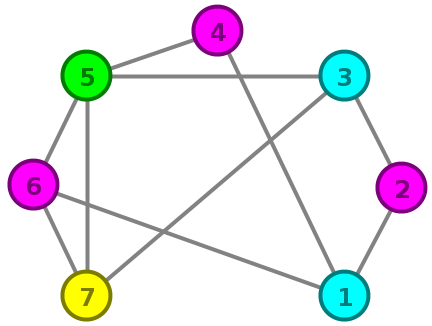
\includegraphics[width=0.45\linewidth]{bad_order_color}
% \hfill
% 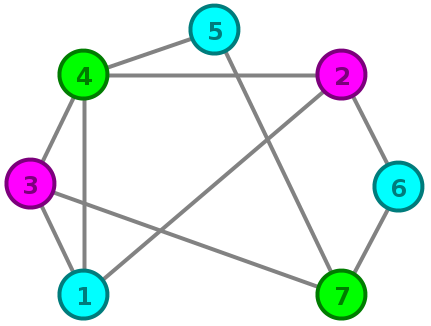
\includegraphics[width=0.45\linewidth]{good_order_color}
%\end{figure}

\begin{figure}
\centering
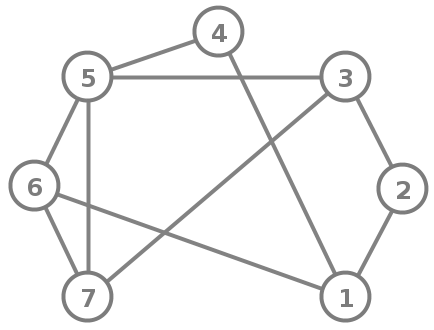
\includegraphics[width=0.28\linewidth]{bad_order}
\hfill
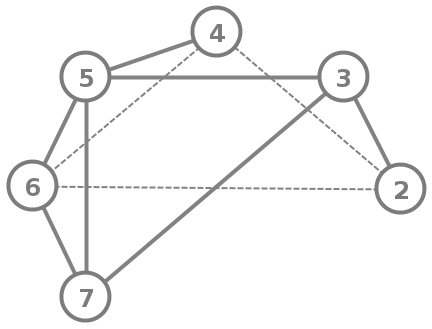
\includegraphics[width=0.28\linewidth]{bad_order_1_removed}
\hfill
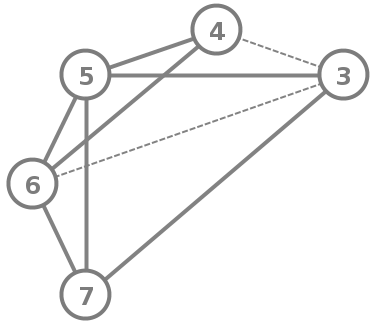
\includegraphics[width=0.23\linewidth]{bad_order_2_1_removed}
\hfill
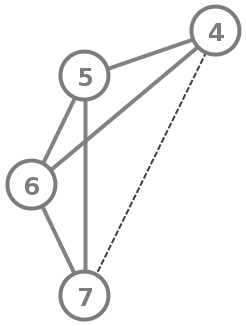
\includegraphics[width=0.16\linewidth]{bad_order_3_2_1_removed}
\caption{A worst case ordering generates $6$ fill-ins. The ordering here is the
numbering which visualized as labels.}
\label{bad_order_fillin}
\end{figure}

Figure~\ref{good_order_fillin} shows how the new ordering produces
$5$ fill-ins when the ordering is $2, 3, 4$. However, the best ordering produces only $3$ fill-ins
as Figure~\ref{good_order_fillin2} shows when the ordering is $2, 5, 3$.

\begin{figure}
\centering
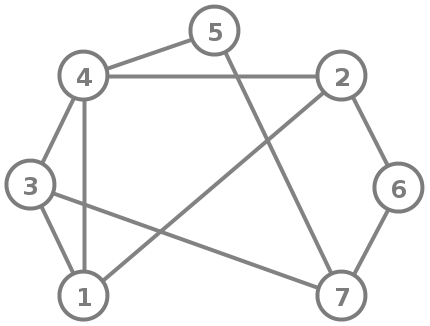
\includegraphics[width=0.28\linewidth]{good_order}
\hfill
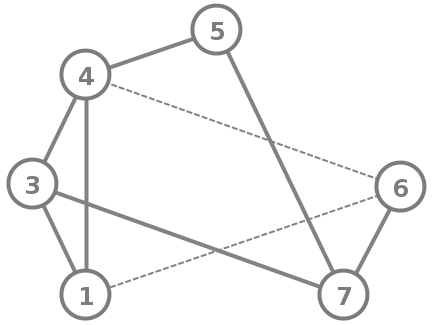
\includegraphics[width=0.28\linewidth]{good_order_2_removed}
\hfill
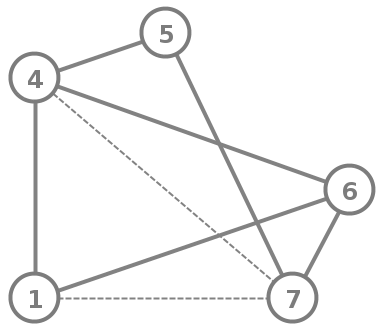
\includegraphics[width=0.23\linewidth]{good_order_3_2}
\hfill
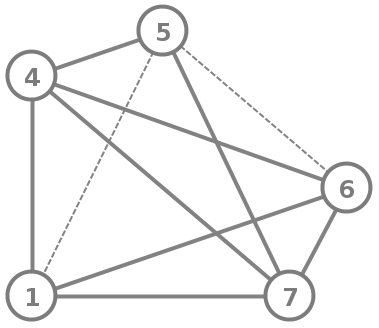
\includegraphics[width=0.16\linewidth]{good_order_4_3_2}
\caption{The order of elimination $2, 3, 4$ generates $5$ fill-ins.}
\label{good_order_fillin}
\end{figure}


\begin{figure}
\centering
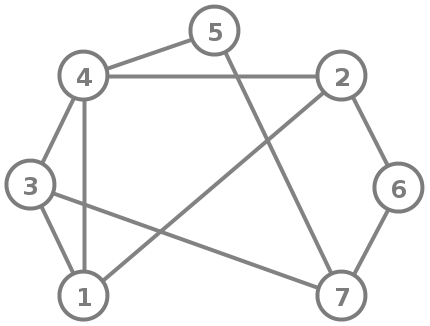
\includegraphics[width=0.27\linewidth]{good_order}
\hfill
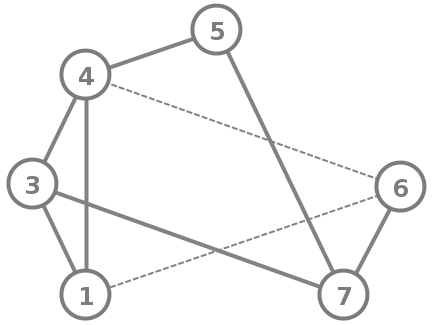
\includegraphics[width=0.27\linewidth]{good_order_2_removed}
\hfill
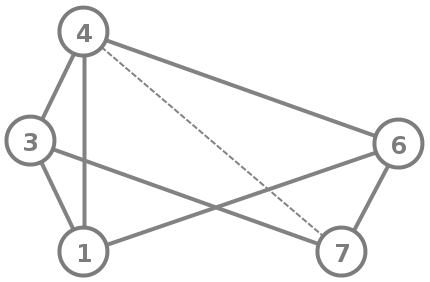
\includegraphics[width=0.23\linewidth]{good_order_5_2_removed}
\hfill
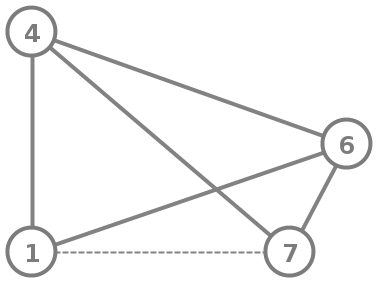
\includegraphics[width=0.18\linewidth]{good_order_3_5_2_removed}
\caption{The order of elimination $2, 5, 3$ generates $3$ fill-ins.}
\label{good_order_fillin2}
\end{figure}

There are various ordering which were studied for coloring heuristics
throughout years.
As we discussed in the previous section, there are different ordering for coloring
like \textit{LFO}, \textit{IDO}, and \textit{SLO}.
%Here, we have a list of such orderings for coloring
%which is available in \textit{PreCol}.
%In each item, we explain how the algorithm select the next vertex.
%\begin{itemize}
%\item Largest-First Ordering (LFO)~\cite{LFO} chooses a vertex with minimum degree in each step.
%\item Incidence-degree Ordering (IDO)~\cite{IDO} chooses first the vertex with maximum degree in $G$, namely $v$. Then, it selects the %matrix with the maximal degree in the subgraph induced by $V(G)-v$. It means the vertex with the maximum incidence degree is selected.
%\item Saturation-degree Ordering (SDO)~\cite{SDO} chooses first the vertex with the maximum degree in $G$, namely $v$. Then, it chooses the vertex with the maximum saturation degree in
%$V$. The saturation degree of the vertex $v$ is the number of different colored vertices in the neighbors of $v$.
%\end{itemize}
In addition to these orderings, we consider three other orderings for preconditioning:
\begin{itemize}
\item Natural Ordering (Nat): This is the natural ordering of the input matrix.
\item Minimum Degree Ordering (Min): The one generates a list of vertices which are sorted based on the degree from minimum to maximum.
\item Metis Ordering\cite{metis,par-nested-disection} (Metis):
This is a fill-reducing ordering based on the algorithm of nested dissection. We use the software \textit{Metis} for generating this ordering.
\end{itemize}
The Table~\ref{ilu-effect} shows how different ordering generates different fill-ins required elements.
The number of fill-ins compared based on the different orderings
for the graph vertices. The number of colors remains the same since we change only the ordering for
ILU factorization.
The left table is the computation for the matrix \textit{nos3.mtx}
and the right one is the computation for the matrix \textit{gyro\_m}.
Both are from the Florida sparse matrix collections.
\begin{table}
\begin{tabular}{|c|c|c|c|c|}
\hline
Orders & Colors & Fill-ins\\\hline
Nat & 15 & 70\\\hline
Min & 15 & 52\\\hline
Metis & 15 & 52\\\hline
\end{tabular}
\hfill
\begin{tabular}{|c|c|c|c|c|}
\hline
Orders & Colors & Fill-ins \\\hline
Nat & 34 & 8760 \\\hline
Min & 34 & 8414 \\\hline
Metis & 34 & 642\\\hline
\end{tabular}
\caption{The number of fill-ins compared based on the different orderings
for the graph vertices. The number of colors remains the same since we change only the ordering for
ILU factorization.
The left table is the computation for the matrix \textit{nos3.mtx}
and the right one the computation is for the matrix \textit{gyro\_m}.
Both are from the Florida sparse matrix collections.}
\label{ilu-effect}
\end{table}

These results are computed on the matrix \textit{nos3.mtx}
and the matrix \textit{gyro\_m} from
the Florida sparse matrix collections. The block size is
chosen to be $50$ for the matrix \textit{gyro\_m} and $15$ for
the matrix \textit{nos3}. Also, the coloring algorithm would be a one-sided
partial coloring. In this table, the fill-reducing Metis ordering
generates the minimum fill-in.
Another observation is that the Metis and Min ordering are generating almost the same
number of fill-ins for the small matrices.
It is only for the big matrices which the efficiency of Metis ordering can be seen.

This difference in the number of fill-ins can affect the convergence speed
relatively. Both Figure~\ref{nat_convergence}
and Figure~\ref{metis_convergence} show
the convergence history of the BICGSTAB solvers on the matrix \textit{nos3}.
The three line charts are the convergence history of the solver with
no preconditioning, ILU preconditioning with block-diagonal sparsification,
and ILU preconditioning with block-diagonal sparsification together with the found
additionally required elements, respectively.
Here, the block size is chosen to be $10$ and the level of ILU factorization
is $10$.
Clearly, Figure~\ref{metis_convergence} has a better convergence rate in the chart
in which the additionally required elements are added in comparison with the same
chart in Figure~\ref{nat_convergence}.

\begin{figure}
\centering
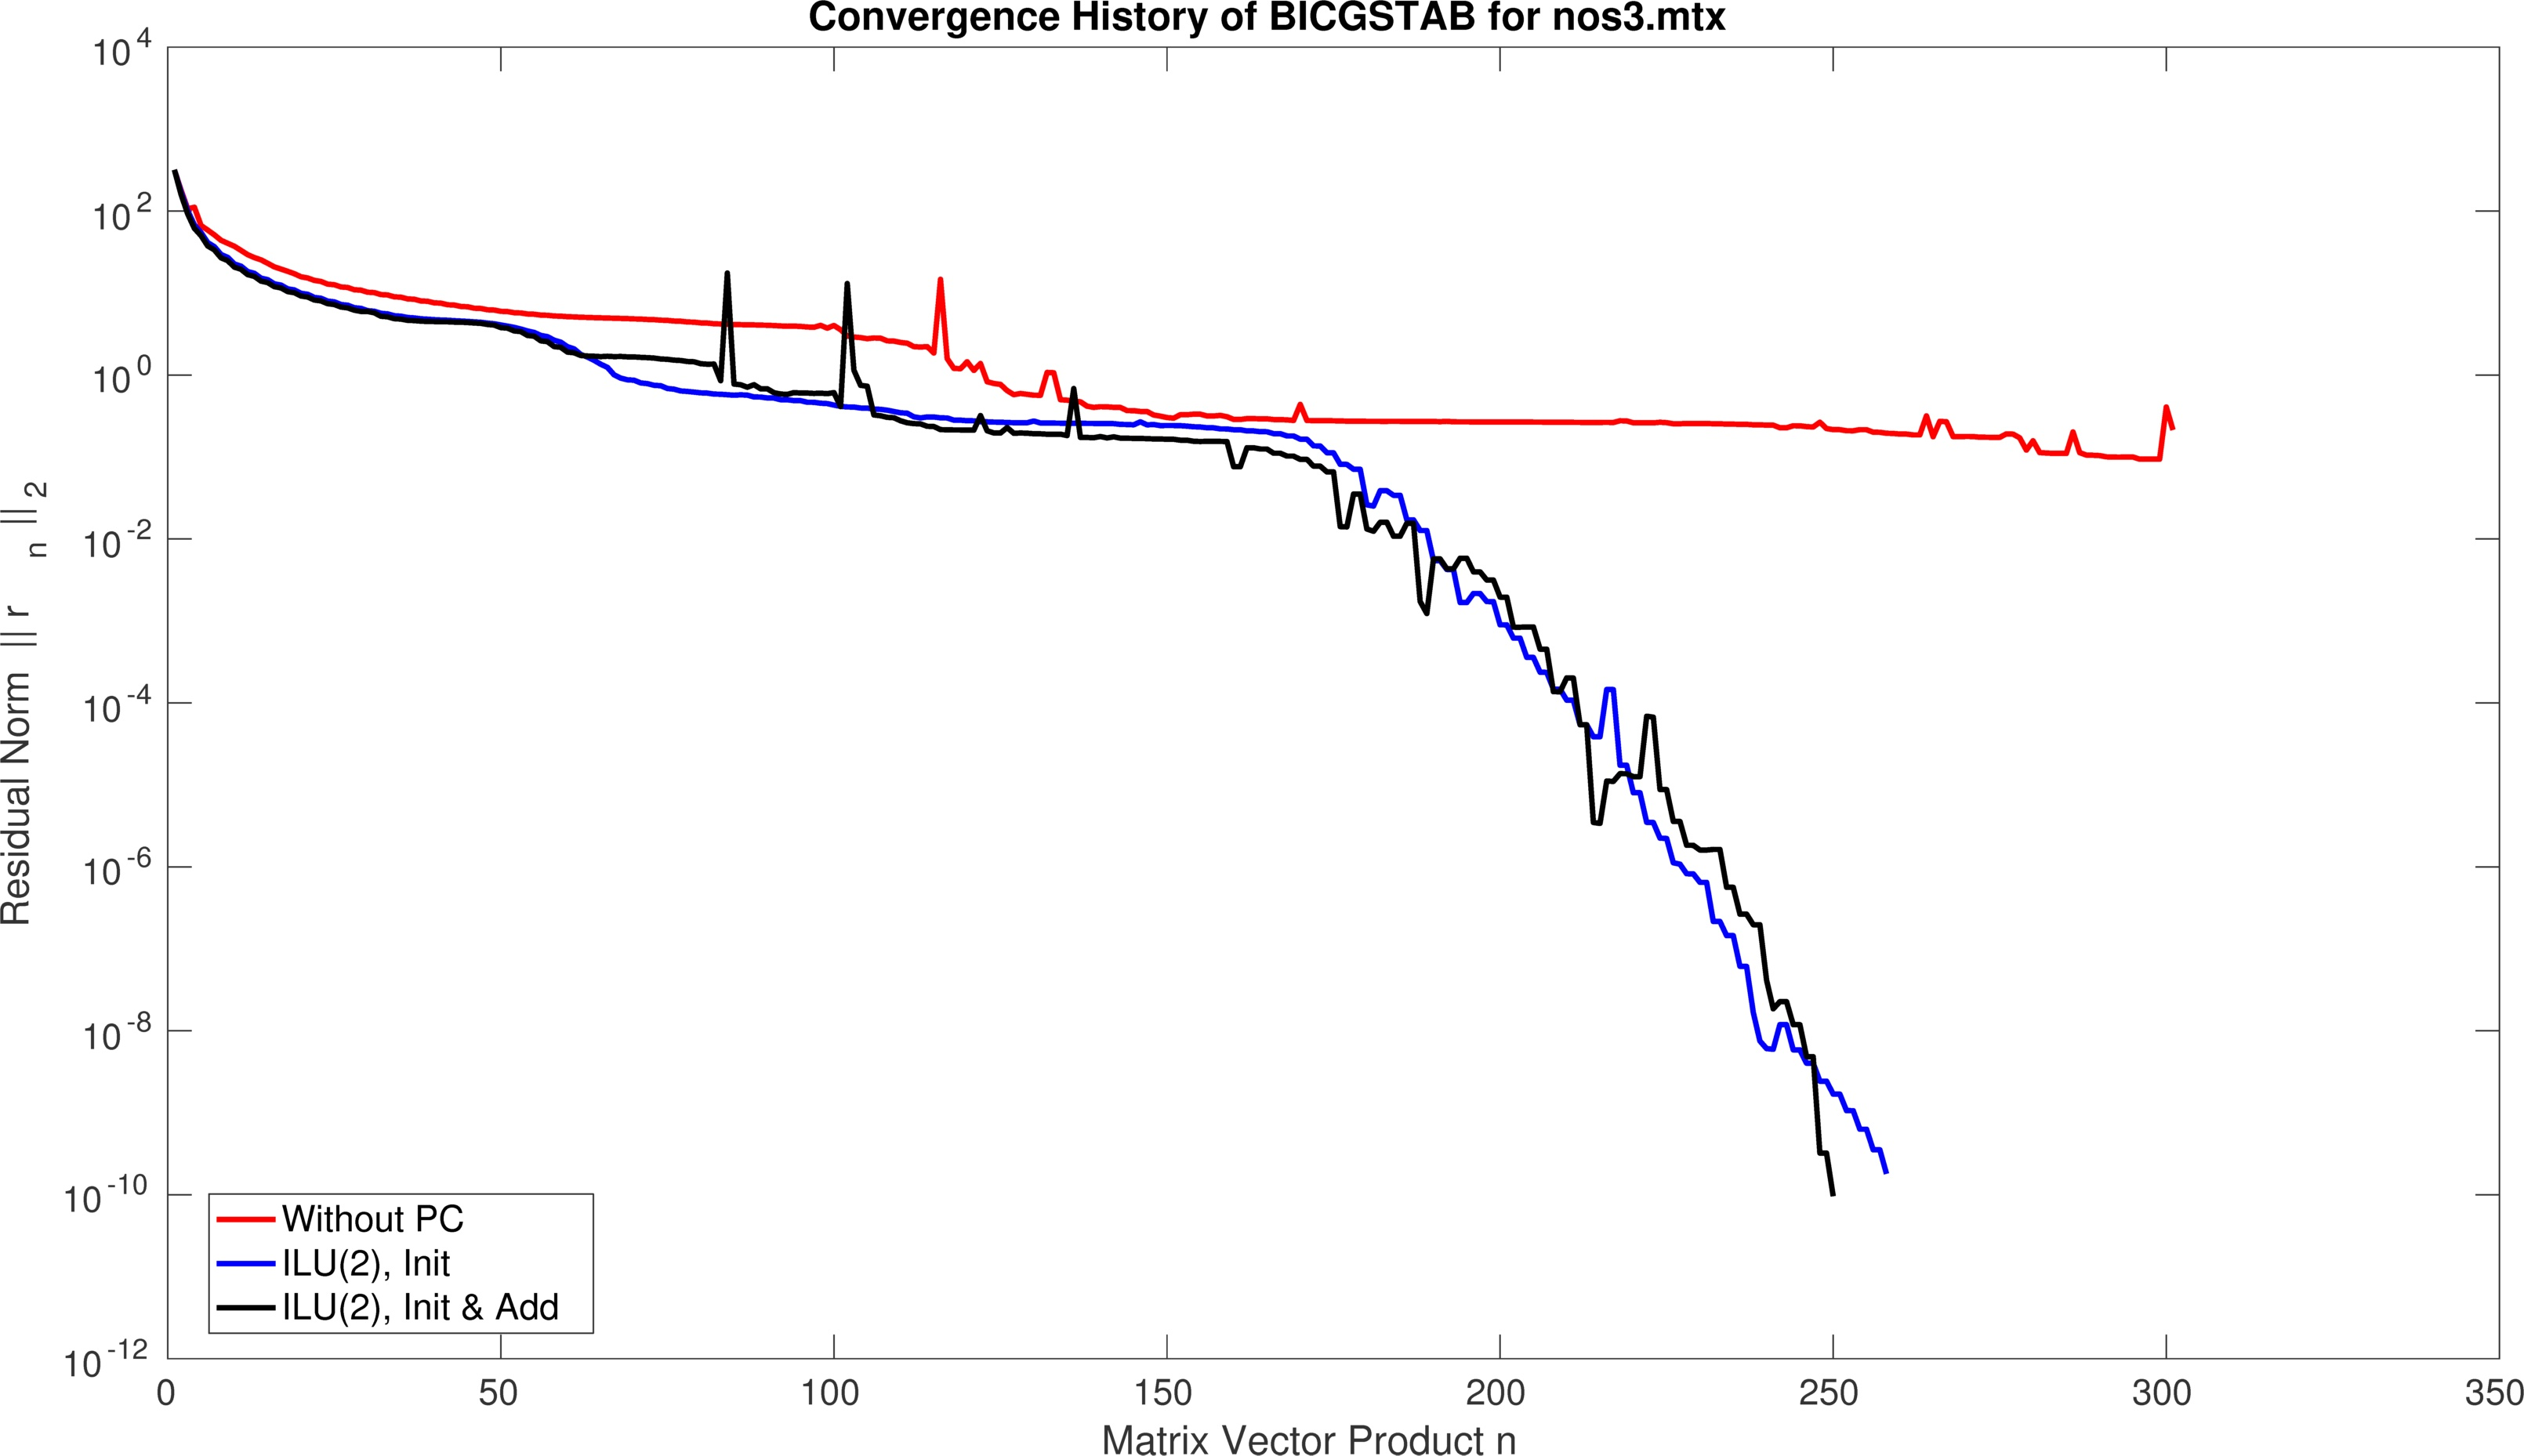
\includegraphics[width=0.9\linewidth]{nos3_mtx_convergence_nat}
\caption{Natural ordering results in a worst convergence.}
\label{nat_convergence}
\end{figure}
\begin{figure}
\centering
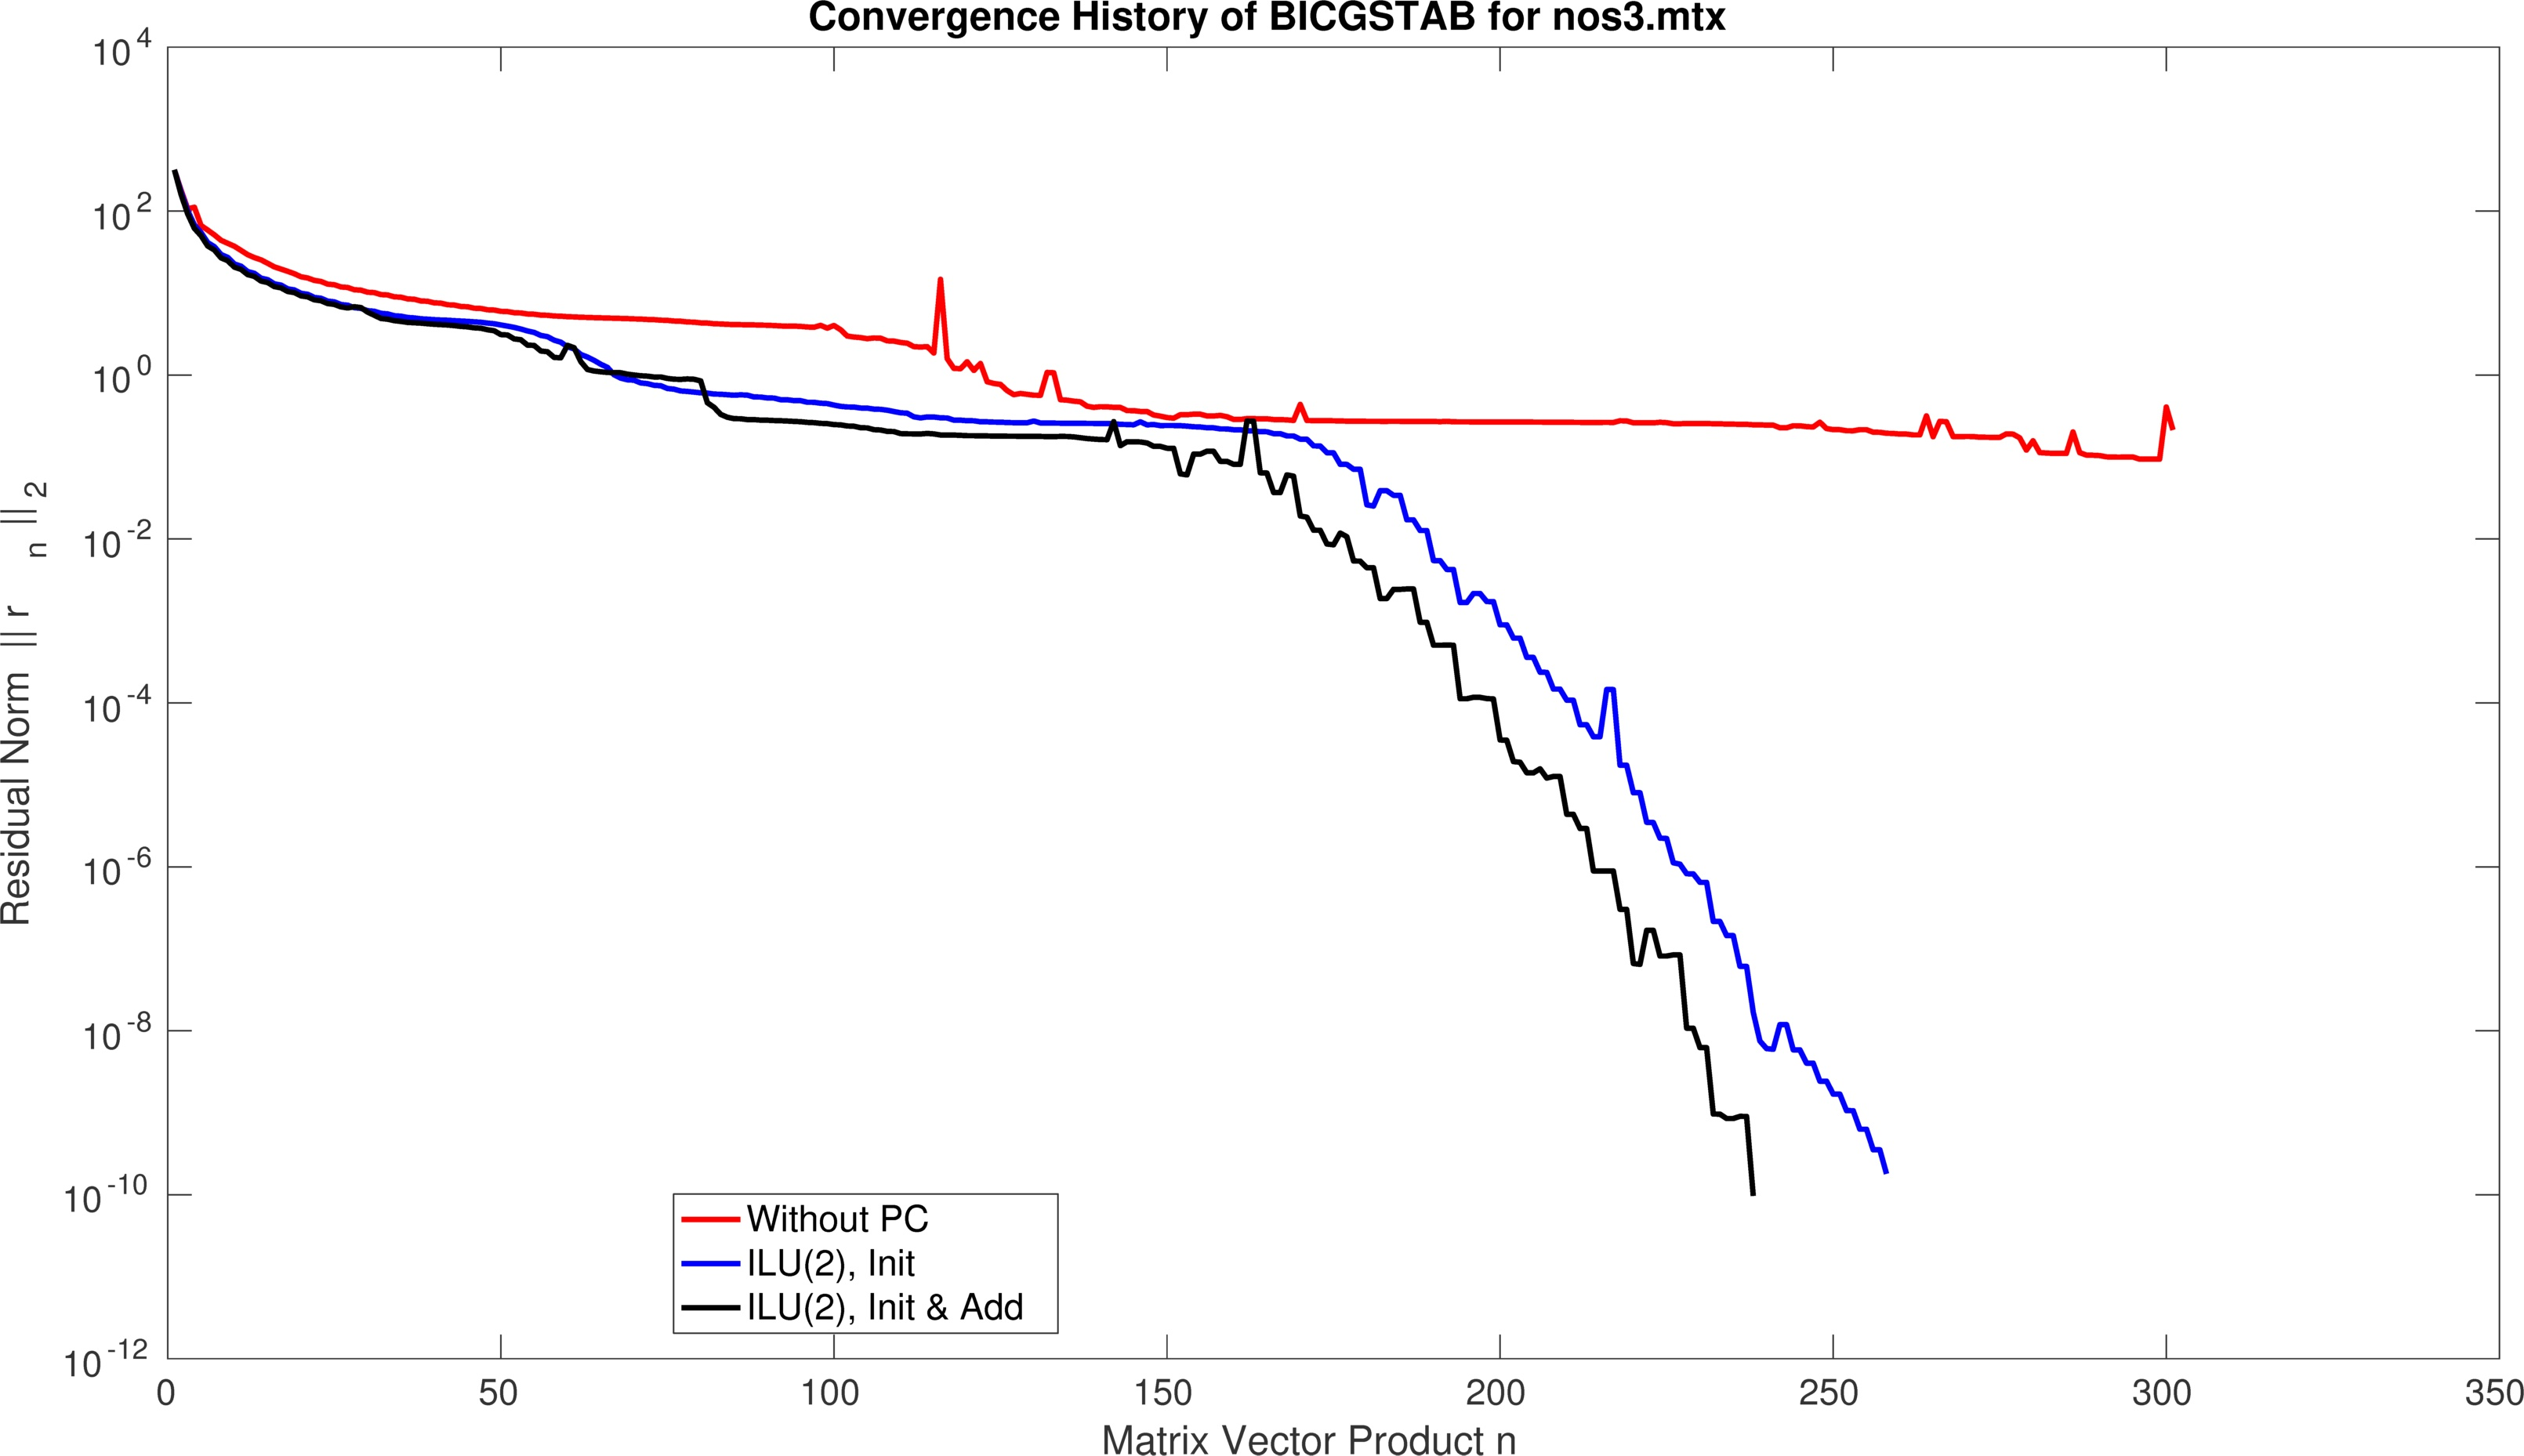
\includegraphics[width=0.9\linewidth]{nos3_mtx_convergence_metis}
\caption{Metis ordering results in a better convergence.}
\label{metis_convergence}
\end{figure}

So far, we decided for the level of ILU factorization arbitrarily.
Here, we want to see the actual influence of the level parameter on
the fill-ins which is visualized in \figref{el_fillins_orderings},
\begin{figure}
\centering
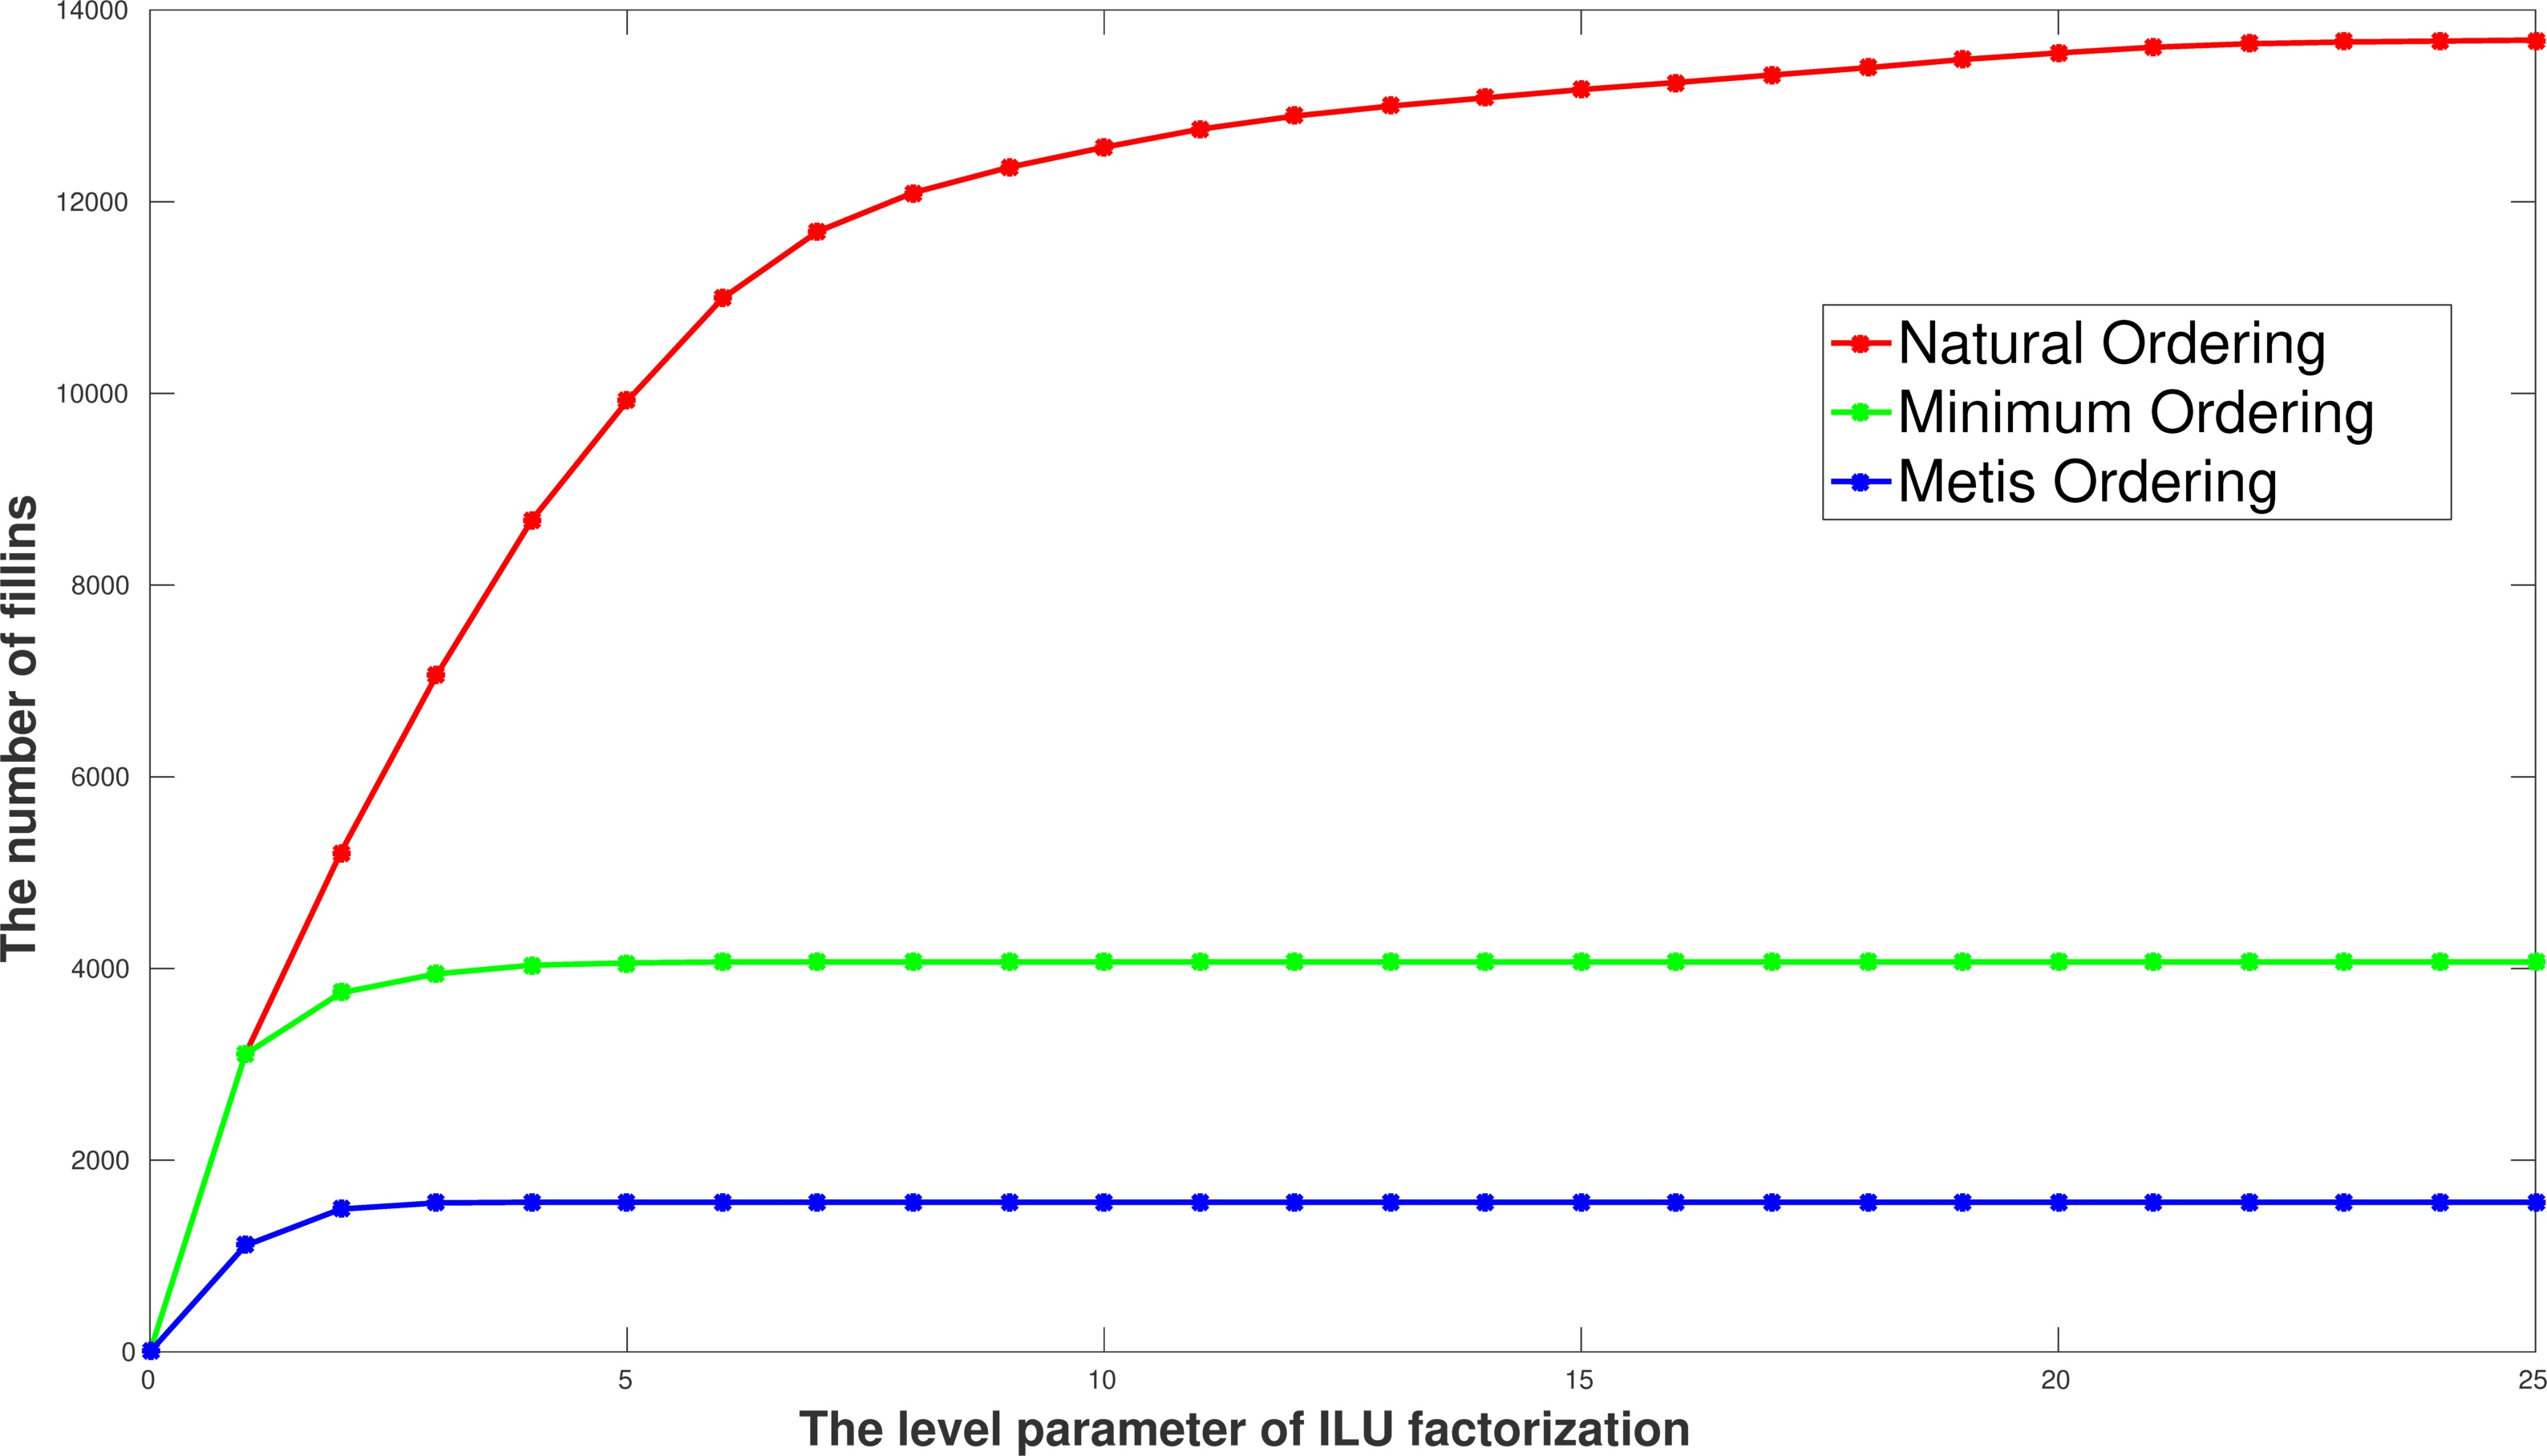
\includegraphics[width=0.9\linewidth]{el_fillins_orderings.jpg}
\caption{The influence of the level parameter for ILU on the number of fill-ins
while three different orderings are employed.
The block size is fixed to $100$.
The matrix is \textit{ex33} and the level parameter changes from $0$ to $25$.
The ordering for coloring is \textit{LFO}.}
\label{el_fillins_orderings}
\end{figure}

\begin{figure}
\centering
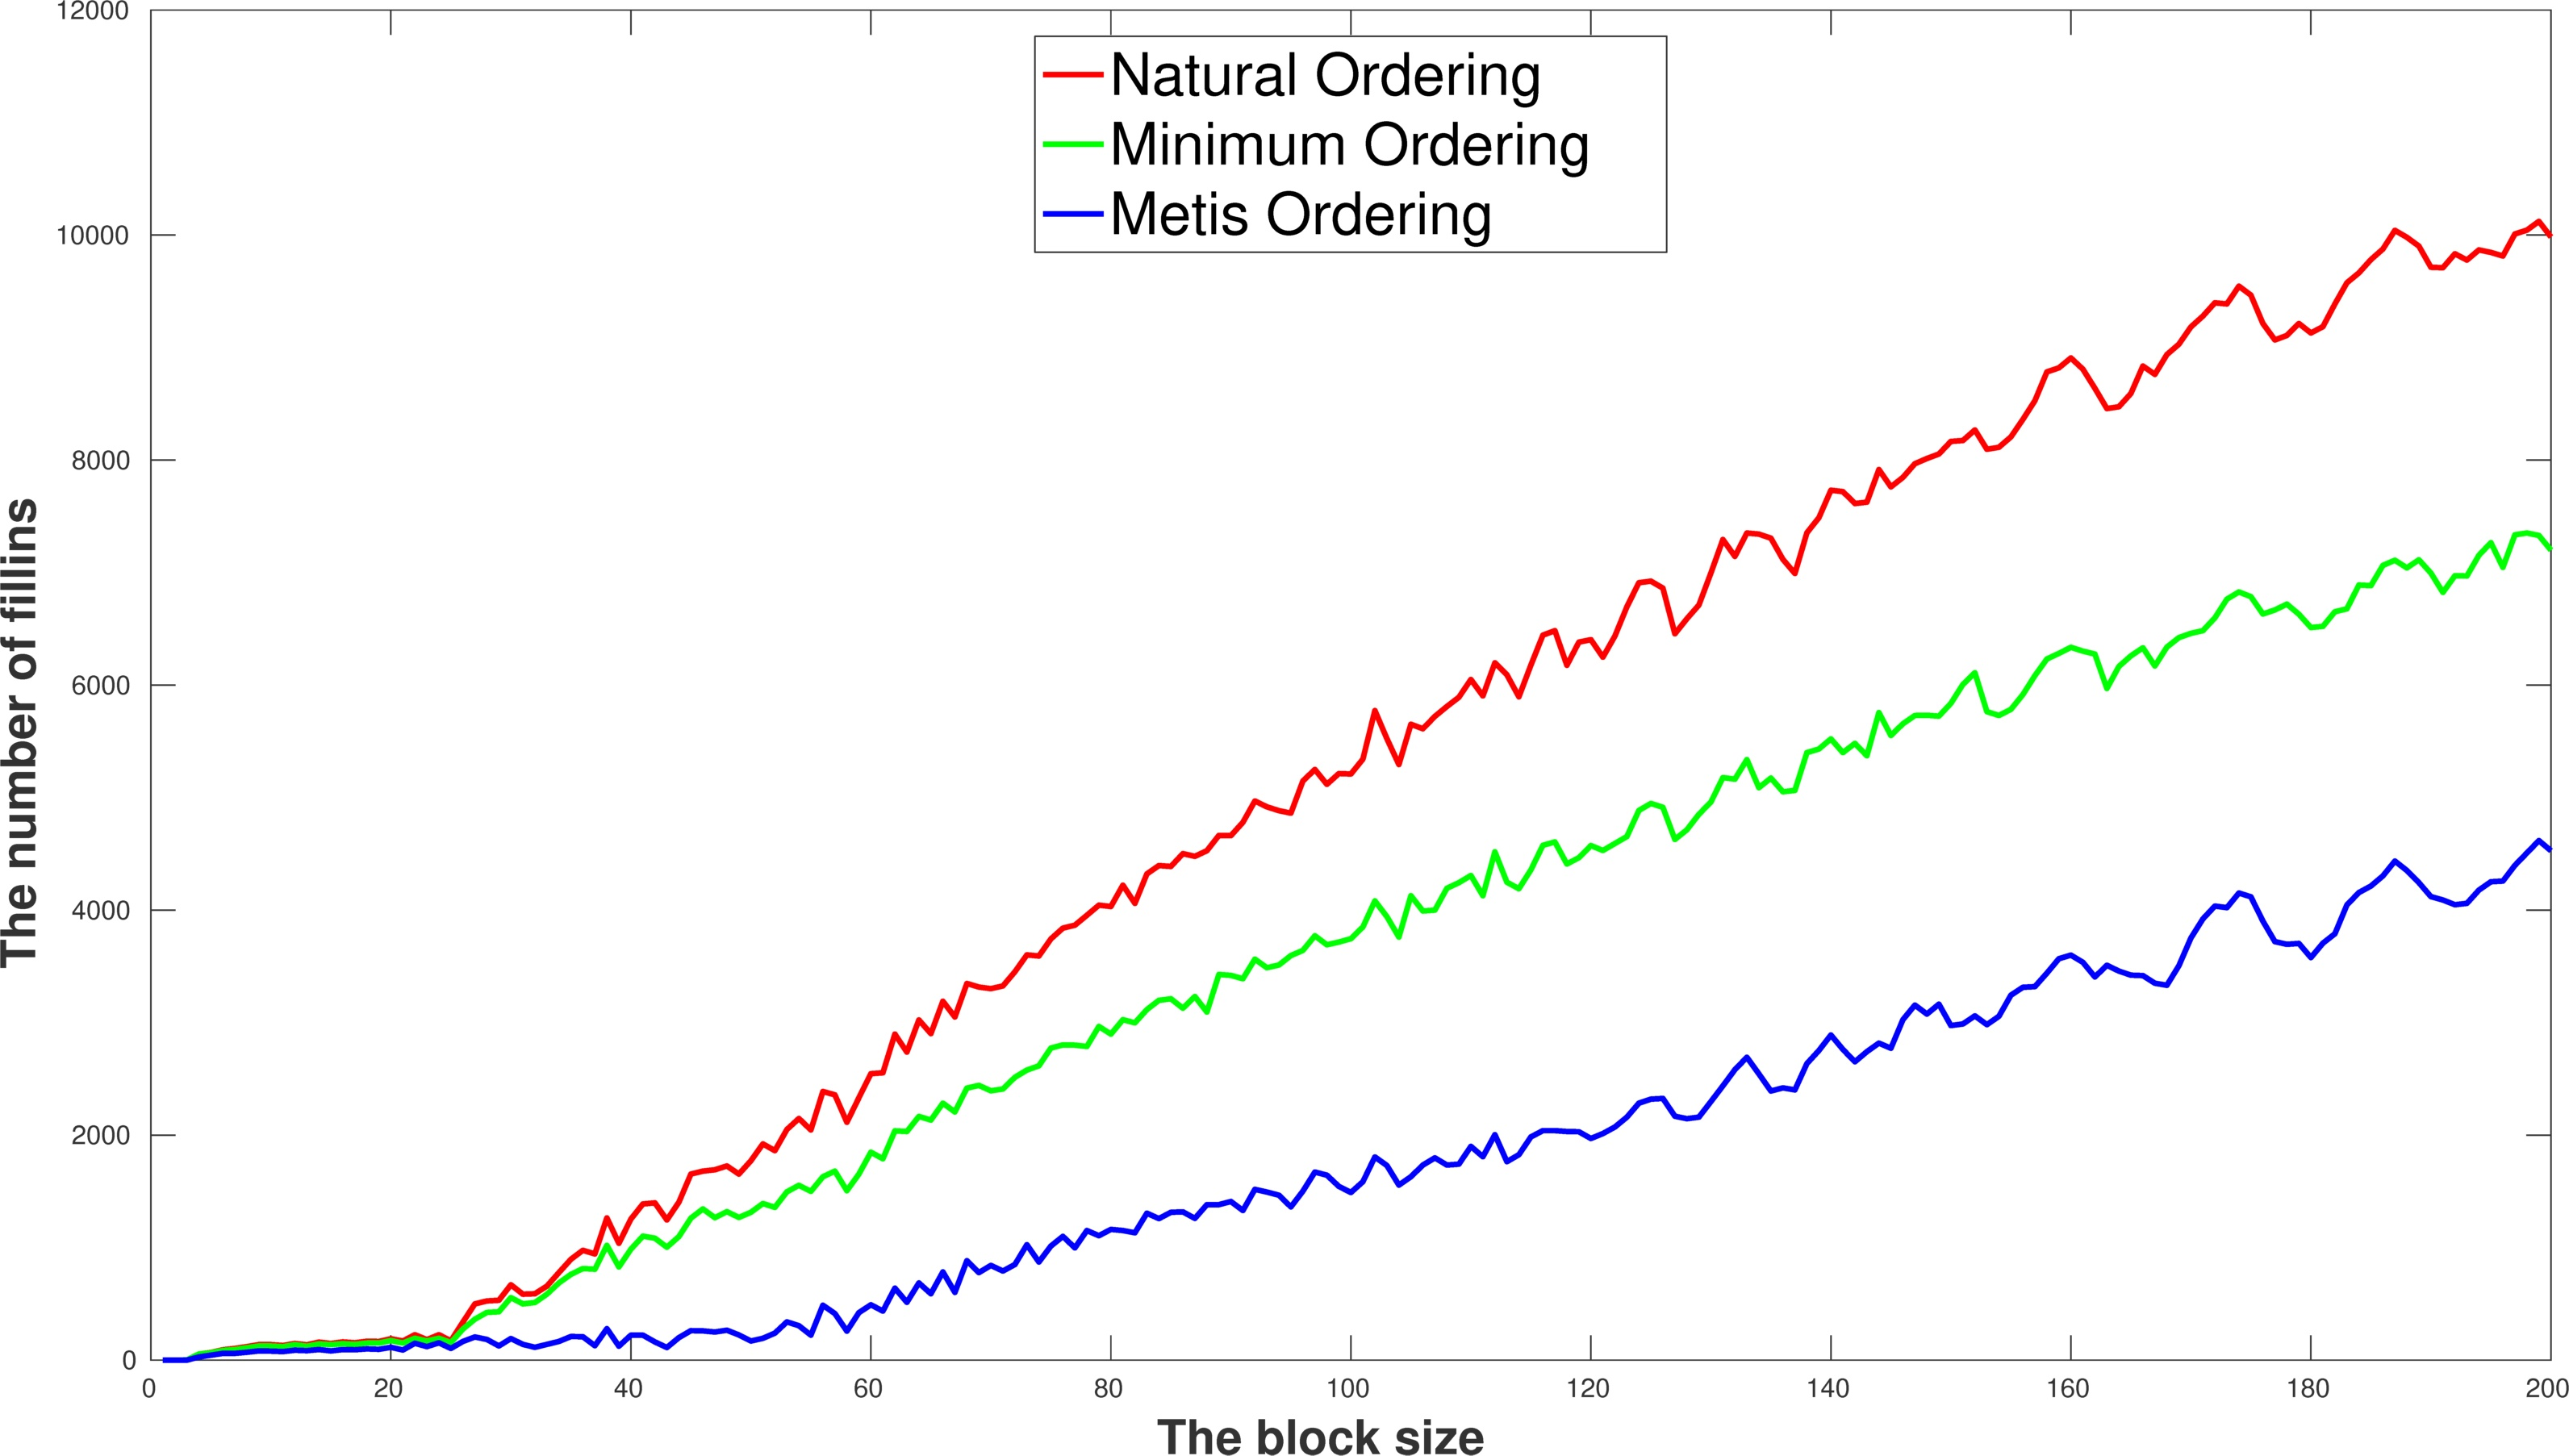
\includegraphics[width=0.9\linewidth]{bls_fillins_orderings.jpg}
\caption{The influence of the block size for sparsification on the number of fill-ins
while three different orderings are employed.
The block size is fixed to $100$.
The matrix is \textit{ex33} and the block size changes from $1$ to $200$.
The ordering for coloring is \textit{LFO}.}
\label{bls_fillins_orderings}
\end{figure}

On the other hand, the coloring has its influence on the number of
additionally required elements. Table~\ref{col-effect}

Here, we did not change any settings other than the ordering of coloring. The ordering for
ILU preconditioning is fixed to the natural ordering.
The block size is $50$ and $10$ and the ILU level is $5$ and $2$ for two matrices
\textit{gyro\_m} and \textit{nos3}, respectively.
The matrix is \textit{gyro\_m}.
\begin{table}
\begin{tabular}{|c|c|c|c|}
\hline
Ordering & Colors & Fill-ins & $|R_a|$ \\\hline
LFO & 34 & 8760 & 66554 \\\hline
SLO & 33 & 8760 & 57760 \\\hline
IDO & 35 & 8760 & 66588 \\\hline
\end{tabular}
\hfill
\begin{tabular}{|c|c|c|c|}
\hline
Ordering & Colors & Fill-ins & $|R_a|$ \\\hline
LFO & 15 & 50 & 394 \\\hline
SLO & 12 & 50 & 384 \\\hline
IDO & 16 & 50 & 436 \\\hline
\end{tabular}
\caption{The effect of coloring on the number of additionally required elements
computed for two matrix \textit{gyro\_m} and \textit{nos3}. }
\label{col-effect}
\end{table}

It can be seen that the number of additionally required elements increases when
the number of colors decreases. This is understood as the number of potentially
required elements are chosen from the non-required elements and added to the required elements
such that number of colors does not increase. Hence, if the number of colors is more,
the freedom of choosing elements gets higher.
As two tables~\ref{ilu-effect} and~\ref{col-effect} shows,
both the ordering of coloring and the ordering of preconditioning affects the number of
additionally required elements. Although smaller number of fill-in increases
the number of additionally required elements, the smaller number of colors
decreases the number of additionally required elements.
This is in contrast to the minimum number of colors which we are searching for,
in the automatic differentiation.

%\subsection{Consdiering the positions of required elements}
%\subsection{Predicting the additionally required elements }

\section{Partial Coloring Restricted to Diagonal Elements}
So far, we consider the partial Jacobian computation with an arbitrary
set of required elements. However, a better heuristics is proposed if the
pattern of the required elements is priori known.

In Lülfesmann~\cite{Lulfesmann2012Fap}, it is shown that the number of colors of
a partial star bicoloring restricted to diagonals is equal to
the minimal number of colors in a partial distance-$2$ coloring restricted
to diagonals. It means the bidirectional compression is not better than
a distance-$2$ coloring.
Looking at the proof, this theorem can be generalized by considering any
coloring instead of the optimal coloring.

On the other hand, the set of diagonal elements in the theorem
can be replaced by any set of required elements
in which each column and row should contain only one required nonzero elements.
This property is nothing than a matching~\cite{bondy2008graph} in a graph language.
Given a graph and the vertex and edge set $G=(V,E)$, a matching $M\subset E$ contains
a list of edges which do not have any vertex in common.
A maximum matching is a matching with a maximum possible number of edges.
Then, a diagonal for example in our bipartite graph is a maximum matching.

Now, we can formulate a new theorem on the comparison of one directional and
bidirectional coloring as follows,
\begin{theorem}
\label{t.matching}
Given the graph $G=(V,E)$ and a matching $M\subset E$ representing
the required elements, any valid partial star bicoloring $Q_{sp}$ restricted to $M$
with the number of colors $\chi_{sp}$
can be transformed to a valid distance-$2$ coloring restricted to $M$
with the number of colors $\chi_{d2}$ such that $\chi_{sp} \leq \chi_{d2}$.
These number of colors can be different than the minimal number of colors.
\end{theorem}
The proof is straightforward and can be found in \appref{app.proof.1}.
Based on the $\sparsifysymbol$-column intersection graph defined in~\defref{d.part.cig},
it is easy to see
that the partial coloring restricted to diagonal is still a NP-complete problem.
We discussed this shortly in \appref{app.npcomp}.
Therefore, we should still use some heuristics to compute these colorings.
The examples in Table~\ref{table.starbic.d2.diag} from Florida sparse collection shows that the
inequality in Theorem~\ref{t.matching} can happen. The second column of this table
shows the number of colors computed by the heurstic for star bicoloring.
The third column shows the number of colors computed by the greedy distance-$2$ coloring
in which the minimum number of colors between the row and column version is selected.
It can be seen that even for a small matrix as the matrix \textit{cage3} which has only
$5$ rows and columns, the star bicoloring can produce a better result.
However, the difference between the number of colors is not so high for these examples.
So, it is not maybe efficient to run the star bicoloring to get a better coloring for
the one-sided coloring. Hence, a new heuristic is proposed with a lower complexity
to compute the same coloring.
\begin{table}
\centering
\begin{tabular}{|c|c|c|}
\hline
Name & $\Phi_{sb}$ & min($\Phi_r$,$\Phi_c$)\\\hline
\textit{cage3} & $3$ & $4$\\\hline
\textit{cage4} & $3$ & $4$ \\\hline
\textit{cage5} & $5$ & $7$\\\hline
\textit{cage7} & $7$  & $8$\\\hline
\textit{cage8} & $8$  & $10$\\\hline
\textit{cage9} & $9$  & $11$\\\hline
\textit{cage10} & $10$ & $11$\\\hline
\textit{cage12} & $13$ &  $14$\\\hline
\end{tabular}
\hfill
\begin{tabular}{|c|c|c|}
\hline
Name & $\Phi_{sb}$ & min($\Phi_r$,$\Phi_c$)\\\hline
\textit{ex7} & $18$ & $22$ \\\hline
\textit{nos3} & $10$ & $10$ \\\hline
\textit{steam1} & $6$ & $6$ \\\hline
\textit{steam2} & $8$ & $8$ \\\hline
\textit{rajat01} & $8$ & $8$ \\\hline
\textit{gyro\_m} & $15$ & $15$\\\hline
\textit{ex33} & $12$ & $11$\\\hline
\textit{cavity16} & $20$ & $18$ \\\hline
\end{tabular}

\caption{The comparison of number of colors in star bicoloring and in
distance-$2$ coloring restricted to diagonals.
The ordering is the natural ordering of the matrix for the both colorings.
%the value of $\alpha$ is equal $1.0$
}
\label{table.starbic.d2.diag}
\end{table}

We have developed some ideas based on Theorem~\ref{t.matching}
for a better heuristic. The idea is that a heuristic for star bicoloring maybe
find a better coloring because of the inequality in the theorem.
As theorem proposes, every required nonzero element
is determined by either a column or a row and not both. Hence, a heuristic
can iterate on the required element and selects between the row and column of
the nonzero in favour of minimal coloring.
Thus, the star bicoloring heuristic can be rewritten for a better computational complexity.
Regarding these ideas, the star bicoloring is rewritten as in \coderef{star.diagonal}.
\begin{figure}
\begin{lstlisting}[
caption=An improved star bicoloring restricted to diagonal elements.
As the theorem says this coloring generates an equivalent distance-$2$ coloring.,
label=star.diagonal,mathescape]
funtion star_diag($G=(V_r\cup V_c)$, $E_R$)
for $v\in V_c$
  $\Phi(v)=-1$
  $forbiddenColors1[v] = 0$
  $forbiddenColors2[v] = 0$

for $e=(v,u)\in E_R$
  $forbiddenColors1[0] = v$
  $forbiddenColors2[0] = u$

  for $n\in N2(G_b,v)$
    if $\Phi(n) > 0$
      $forbiddenColors1[\Phi(n)] = v$

  forbiddenColors[0] = u;
  for $n\in N2(G_b,u)$
    if $\Phi(n) > 0$
      $forbiddenColors2[\Phi(n)] = u$

  $c_1 = min(\{j>0: forbiddenColors1[j] \neq v\})$
  $c_2 = min(\{j>0: forbiddenColors2[j] \neq u\})$

  if $c_1 < c_2$
    $\Phi(v) = c_1$
  else
    $\Phi(u) = c_2$

  for $v\in V_c$ with $\Phi(v)>0$
    $\Phi(v) = \Phi(v) + max(\{ \Phi(u):u\in V_r \})$

  for $v\in V_r\cup V_c$ with $\Phi(v) = -1$
    $\Phi(v) = 0$
\end{lstlisting}
\end{figure}
\section{Parallelization}
\label{s.parallel}
As we saw in \secref{s.precond}, different steps should be followed
to compute the additionally required elements. Here, we look at each of
these steps and examine how they can be parallelized by OpenMP
if it can be done efficiently.

First, we look at the coloring algorithm.
There are many literature for a parallelized coloring algorithm.
For example,
{\c{C}}ataly{\"{u}}rek~\cite{cataly2012} itroduced an OpenMP parallelized
algorithm which comptues the same number of colors as the serial version.
However, there are two points in each step of the algorithm in which two threads
need to be synchronized.
However, we focus on another algorithm from Rokos et al~\cite{Rokos2015}
which presents an algorithm in which only a point of synchronization is
needed. The number of colors also remains near to the number of colors
in the serial version. A bipartite version of the algorithm can be easily
adapted as in \coderef{omp.greedy.bip}. This algorithm first colors the vertices
greedily and then corrects the false colorings which can happen.
\begin{figure}
\begin{lstlisting}[caption=A OpenMP parallelized version of greedy algorithm
adapted for the bipartite graph.,label=omp.greedy.bip,mathescape]
function d2_color_omp($G$,$V$)
#progrma omp parallel for
for $v\in V$
$forbiddenColors[\Phi(n)] = v$
$\Phi(v) = min \{ a>0:forbiddenColor[a]\neq v\}$
#pragma omp barrier
$U_0 = V$
$i = 1$
while $U_{i-1}\neq \emptyset$
$L=\emptyset$
#pragma omp parallel for
for $v\in U_{i-1}$
if $\exists u\in N_2(v), u>v: \Phi(u) = \Phi(v)$
$forbiddenColors[\Phi(n)] = v$
$\Phi(v) = min \{ a>0:forbiddenColor[a]\neq v\}$
#pragma omp barrier
$U_i = L$
$i = i+1$
\end{lstlisting}
\end{figure}
This idea of parallelization can be applied to our new coloring heuristics.
It means we compute the coloring like before by a parallelized loop.
Then, we correct the coloring. \coderef{code.new.bip.omp} shows the parallelized
version of \coderef{omp.greedy.bip}.
\begin{figure}
\begin{lstlisting}[caption=New coloring heuristic in the bipartite graph model
parallelized by OpenMP,label=code.new.bip.omp,mathescape]
function d2_color_nreq($G_b$,$\alpha$)
#progrma omp parallel for
for $v\in V_c$ with $\Phi(v)=0$
$forbiddenColors[0] = v$
if $\exists n\in N_2(v): (v,n)\in E_i$
for $n\in N_2(v)$
if $\Phi(n) \neq 0$
$forbiddenColors[\Phi(n)] = v$

$\Phi(v) = min \{ a>0:forbiddenColor[a]\neq v$
$I_v=\{u\in V_c: u\notin N_2(v)\}$
$nreq_v = \{n\in N_2(v):(n,v)\notin E_i\}$
for $i \in I_v$
$nreq_i = \{n\in N_2(i):(n,i)\notin E_i\}$
$req_i = \{n\in N_2(i):(n,i)\in E_i\}$
$mapVtoNreq = mapVtoNreq \cup (i , count (nreq_i - nreq_v))$
$mapVtoreq = map \cup (i , count (req_i))$
$maxs = \{ a\in keys(map): map[a] = max(values(mapVtoNreq))\}$
$mins = \{ a\in keys(map): map[a] = min(values(mapVtoNreq))\}$
$minReq = \{ a\in maxs: mapVtoreq[a] = min(values(mapVtoreq))\}$
$\Phi(minReq) = \Phi(v)$
for $i\in\{0,1,...,\alpha\}$
$\Phi(mins[i]) = \Phi(v)$

#pragma omp barrier
$U_0 = V$
$i = 1$
while $U_{i-1}\neq \emptyset$
$L=\emptyset$
#pragma omp parallel for
for $v\in U_{i-1}$
if $\exists u\in N_2(v), u>v: \Phi(u) = \Phi(v)$
$forbiddenColors[\Phi(n)] = v$
$\Phi(v) = min \{ a>0:forbiddenColor[a]\neq v$
#pragma omp barrier
$U_i = L$
$i = i+1$
\end{lstlisting}
\end{figure}

We color the bipartite graph interpreted from the matrix \textit{Cavity16}
from the sparse matrix collection of University of Florida.
The timing are all from the computation carried on an Intel Core i5 with 8 Gb RAM.
Table~\ref{omp.res} shows the results of this computation.
Here, we change the number of threads from $1$ to $10$ shown in the first column.
The second colum shows the computation time in milliseconds. The third column
is also the number of colors which changes based on the number of colors.
Table~\ref{omp.res}(Left) shows the results of computation of \coderef{omp.greedy.bip}
and Table~\ref{omp.res}(Right) for \coderef{code.new.bip.omp}.
Also \figref{speedups} (Left) and \figref{speedups} (Right) visualize the speedup
based on the number of threads.
\begin{figure}
\begin{tabular}{|c|c|c|}
\hline
Threads & Time & Colors \\\hline
1 & 42.8745 & 47 \\\hline
2 & 33.9665 & 47 \\\hline
3 & 25.2741 & 48 \\\hline
4 & 20.6863 & 48 \\\hline
5 & 21.4943 & 47 \\\hline
6 & 20.1796 & 50 \\\hline
7 & 17.9640 & 49 \\\hline
8 & 16.1068 & 52 \\\hline
9 & 15.4174 & 47 \\\hline
10 & 16.1545 & 47 \\\hline
\end{tabular}\hfill
\begin{tabular}{|c|c|c|}
\hline
Threads & Time & Colors \\\hline
1 & 96.795 & 48 \\\hline
2 & 75.744 & 47 \\\hline
3 & 55.605 & 49 \\\hline
4 & 49.335 & 49 \\\hline
5 & 49.360 & 47 \\\hline
6 & 49.365 & 51 \\\hline
7 & 45.342 & 47 \\\hline
8 & 43.254 & 51 \\\hline
9 & 40.742 & 48 \\\hline
10 & 39.416 & 47 \\\hline
\end{tabular}
\caption{
(Left) The results of computation of greedy coloring parallelized by OpenMP.
(Right) The results of computation of new heuristics parallelized by OpenMP}
\label{omp.res}
\end{figure}

\begin{figure}
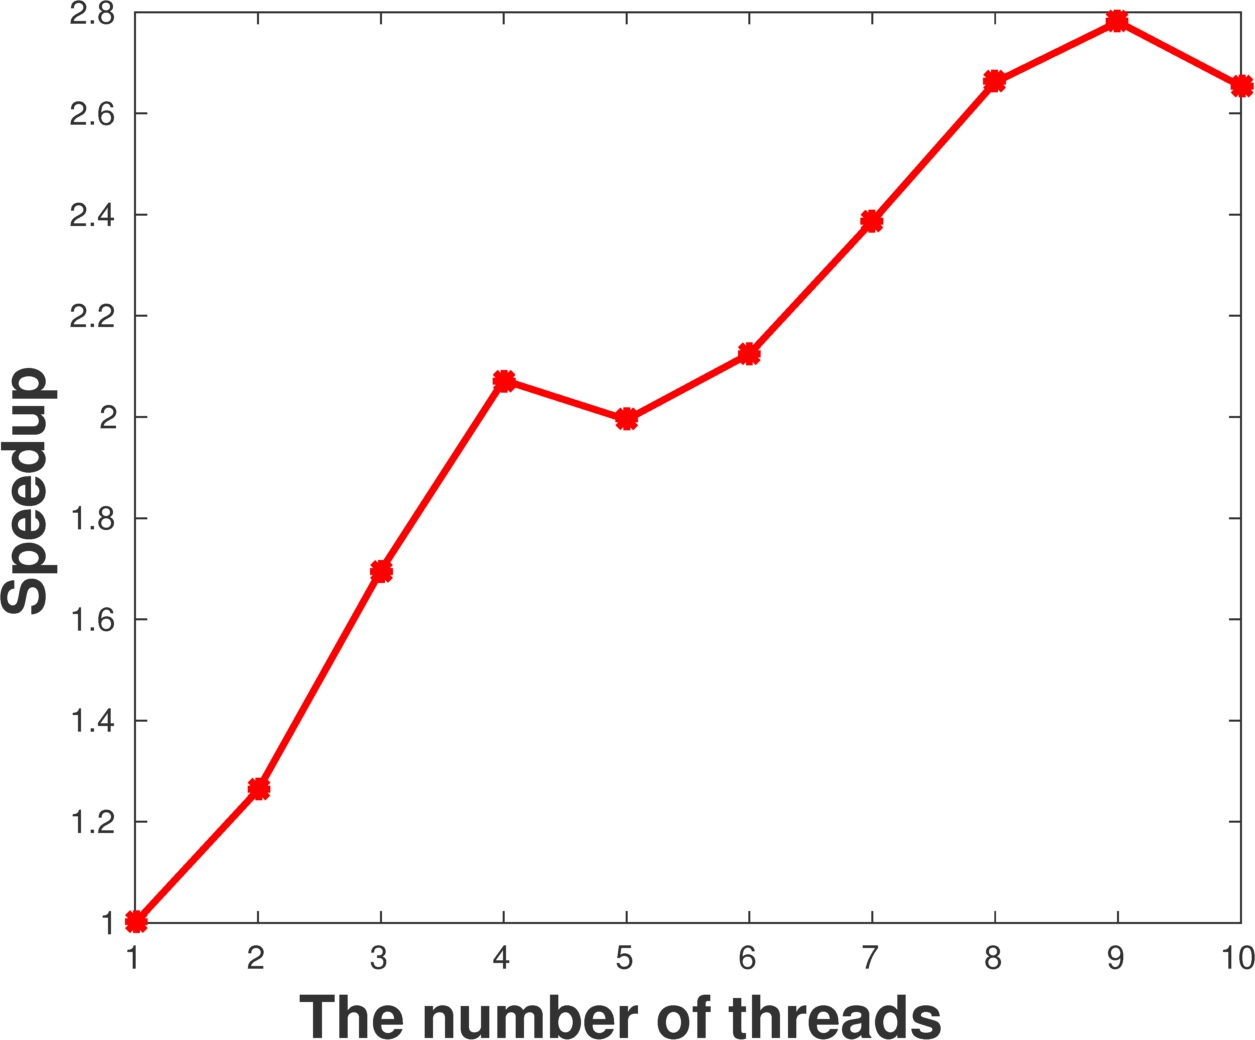
\includegraphics[width=0.44\linewidth]{ths_spd.jpg}\hfill
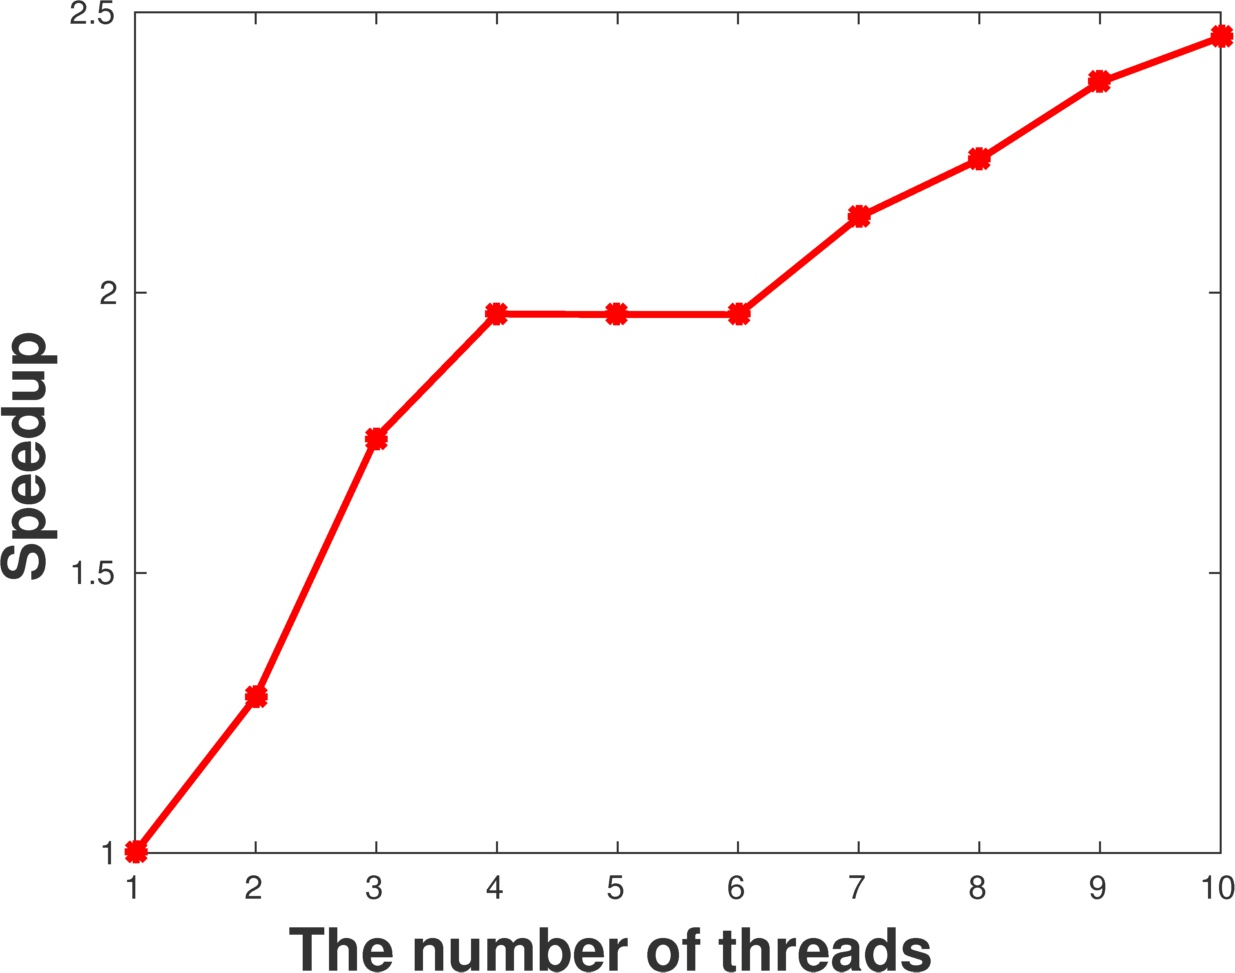
\includegraphics[width=0.47\linewidth]{ths_spd2.jpg}
\caption{
(Left) Speedup for the computation of greedy coloring in bipartite graph model parallelized by OpenMP.
(Right)Speedup for the computation of new coloring heurtistic in bipartite graph model parallelized by OpenMP.
}
\label{speedups}
\end{figure}

This idea can be applied to the new heuristic for star bicoloring which is a potential future work.
Apart from the parallelization of coloring, the block diagonal sparsification makes a suitable
matrix for parallelization. It is well known the fill-ins are generated only in the nonzero blocks in such matrices. This observation gives a direct idea of parallelization in which each process
works on each block. We do not go into details since it is already discussed in previous literature like~\cite{parblockilu}. However, it does not mean that the same idea can be applied in computation of
additionally required elements since those elements are outside the blocks.

%\cite{mpi_greedy_coloring}
%%%%%%%%%%%%%%%%%%%%%%%%%%%%%%%%%%%%%%%%%%%%%%%%%%%%%%%%%%%%%%%%%%%%%%%%%%%%%
\section{PreCol 1.0}
\label{s.extend}
%%%%%%%%%%%%%%%%%%%%%%%%%%%%%%%%%%%%%%%%%%%%%%%%%%%%%%%%%%%%%%%%%%%%%%%%%%%%%
We develop a software to compute the different algorihtm that we propose here.
Specially, the software is designed employing concepts from the object-oriented programming
such that it can be extended later with any new coloring heuristc as well as any preconditioning algorithm.
The developers can implement new extensions without going into details of core implementation.
This is explained in \secref{s.new.ext}.

%%%%%%%%%%%%%%%%%%%%%%%%%%%%%%%%%%%%%%%%%%%%%%%%%%%%%%%%%%%%%%%%%%%%%%%%%%%%%
\subsection{Developer Manual}
\label{s.new.ext}
%%%%%%%%%%%%%%%%%%%%%%%%%%%%%%%%%%%%%%%%%%%%%%%%%%%%%%%%%%%%%%%%%%%%%%%%%%%%%
Two main ingredients coloring and orderings can be implemented now only by deriving an interface.
For example, a new coloring and ordering can be added as easy as the following code.
\begin{lstlisting}
class New_Ordering : public Ordering {
  bool order(const Graph &G_b, vector<unsigned int> &ord, bool restricted) {...}
};

class New_Coloring : public ColAlg {
  int color() {...}
};
\end{lstlisting}

The developer needs to implement this new class in an only-header fashion~\cite{headeronly},
since the goal is to write an extension with a few code. So, the developer should
move the new header file to the corresponding directory which is the ordering directory
for this new ordering and \textit{algs} directory for coloring algorithms.
Now, building the software would bring this new ordering into the software execution.

Using the standard library of C++ as well as the concept of functional programming
in new C++ release~\cite{Sutherland2015}, we provide different functions which can be used
by developer to work on graphs. For example, the iteration of vertices
or edges can be easy as follows,
\begin{lstlisting}
for_each_v(G, f);
for_each_v(G, [&](Ver v) {...});
for_each_e(G, f);
for_each_e(G, [&](Edge e) {...});
\end{lstlisting}
, in which the variable $f$ is a function which gets an input parameter
of a vertex or an edge, respectively.
Also, the other syntax is the lambda function
from the new C++ functional programming to implement a function in place.

Following a unique solution, we implement all the possible part of algorithms
with the use of standard library of C++ which also improves the readability.
This strategy reduces the amount of the code dramatically and
make the code more readable.
Also, the standard algorithms would be automatically parallel in the next
release of C++ (C++17) next year~\cite{parallelcpp}.
%%%%%%%%%%%%%%%%%%%%%%%%%%%%%%%%%%%%%%%%%%%%%%%%%%%%%%%%%%%%%%%%%%%%%%%%%%%%%%%%%%%%%%%%%%%%%%%
\subsection{Software Design}
\label{s.software.design}
%%%%%%%%%%%%%%%%%%%%%%%%%%%%%%%%%%%%%%%%%%%%%%%%%%%%%%%%%%%%%%%%%%%%%%%%%%%%%%%%%%%%%%%%%%%%%%%
This is illustrated in Figure~\ref{f.structure} (Left).
This results in the lack of efficiency. On the other hand,
this mix of programming languages reduces
the accuracy and makes the versioning difficult.
%-----------------------------------------------------------------------------------------------
\begin{figure}
\centering
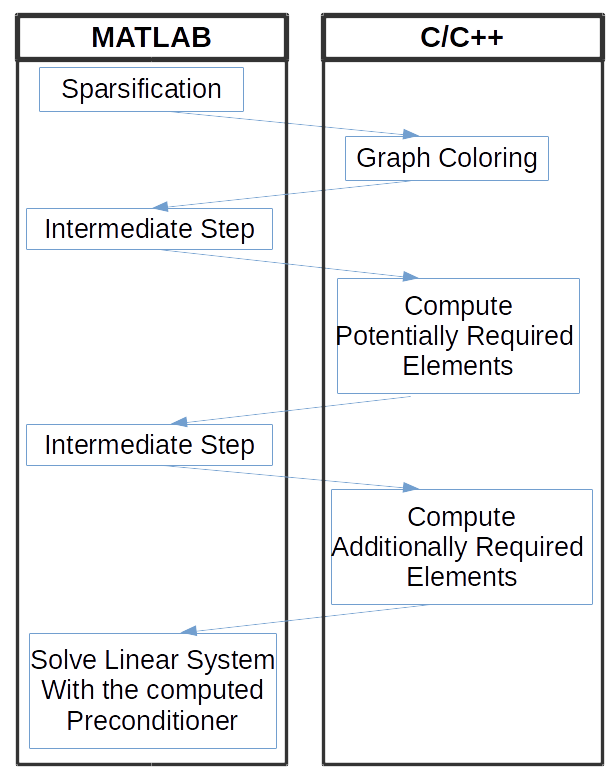
\includegraphics[width=0.42\textwidth]{old_struct}
\hfill
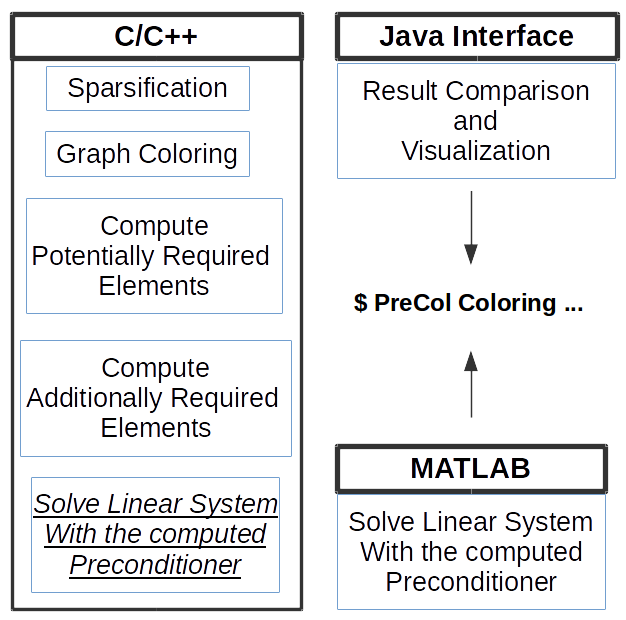
\includegraphics[width=0.52\textwidth]{new_struct}
\caption{There were many communications between MATLAB and C/C++ version. The communication
is done based on the MEX interface. A conversion from matrix to graph is computed
each time that the MEX interface is used. (Left) A new implementation reduces a lot of communication.
It brings together different parts of algorithm in a package. Two interfaces written
in MATLAB and Java call this package as a local program.}
\label{f.structure}
\end{figure}
%-----------------------------------------------------------------------------------------------

We improved the design of the software to resolve these problems.
So, all the parts of the algorithm are computed in \textit{C++} now.
Figure~\ref{f.structure} (Left) visualizes this new implementation.
All the parts can be computed in C++. However,
the part of iterative solver can also be computed in MATLAB.
The MATLAB functions in this area are in general more convincing.
For this goal, we implemented the preconditioning and the sparsification in C++.
As you can see in Figure~\ref{f.structure} (Left), we also introduced
two interfaces in MATLAB and JAVA languages which we will explain in
Section~\ref{s.interfaces}.

To use the software, the user can use a command-line command in addition to
the interfaces in JAVA and MATLAB. So, the user needs to specify different
options for coloring algorithm, orderings, the block size, and so.
These options can be entered directly in the terminal together with command
or can be written in a so called config file which is imported by the software.
The format of config file is as follows,
\begin{lstlisting}
alg: PartialD2Coloring
col_ord: Min
ilu_ord: LFO
type: BlockDiagonal
blk: 10
\end{lstlisting}
Different parameters possible in config file is as follows,
\begin{itemize}
\item alg:
\item col\_ord:
\item type:
\item blk:
\end{itemize}

We also generated a new documentation as a website which is available
under the website: http://csc.c3e.de/precol/html.
This website is generated automatically by Doxygen~\cite{Lischner2013}.
We implemented some new HTML/CSS template for doxygen to include extra
texts and documentation in the website.

\todo{zero or one}
mohem ... discussion about the sparsification in MATLAB and C/C++
staring from zero or one ???


\subsection{User interfaces}
\label{s.interfaces}
\textbf{JAVA interface.}
We extend our JAVA software GraphTea~
\cite{2014:07,2014:15,2014:16,2015:05,2015:06,2015:07,2015:08} to have a
set of reports for graph coloring and preconditioning. It has two different modes
to compute independently or to compute by calling the software \textit{PreCol}.
%Chemical Graph theory\cite{2015:05,2015:06,2015:07,2015:08}
GraphTea is a graph editing framework designed specifically to compute and visualize
different parameters of graphs interactively.
Figure~\ref{f.graphtea} shows a snapshot of the main
graph window together with two additional windows that give more details on the solution
of different graph problems. These separate windows providing additional information are
called ``reports.''

A report can be computed in GraphTea in two different ways:
a single report or an incremental report.
A single report means to compute some parameters on graph and look at the results
in a textual way. However, an incremental report happens when we have at least
two parameter for computation. So, we would change one of the parameter in
some range and would generate a table.

The main goal of developing GraphTea was to help the researcher through their research.
The following abilities of GraphTea could help the research in different dimensions:
\begin{itemize}
\item Generate different class of graphs and compute the parameters on them.
\item Get reports on the graph beside the parameter and find the connections.
\item Compute the operations on graphs and influence of these operations on parameters
of the graph.
\end{itemize}

If we divide the researcher's works follows,
\begin{enumerate}
\item Guess a hypothesis like a bound for coloring number
\item Evaluate this bound on different graphs
\item Prove the hypothesis
\end{enumerate}
The second step, i.e. evaluation, is always an important step since many first errors and
improvements could be found.
However, the researcher can only do this evaluation for small examples if they do not
use computer tools.
Different aspects of GraphTea can be used to overcome this evaluation.
The researchers can generate any graph up to any computationally-reasonable size
(i.e. commutable in a reasonable time) and compute the parameter.
This process of so-called conjecture checking on different graphs could often lead to a better guess.
%-----------------------------------------------------------------------------------------------
\begin{figure}
\centering
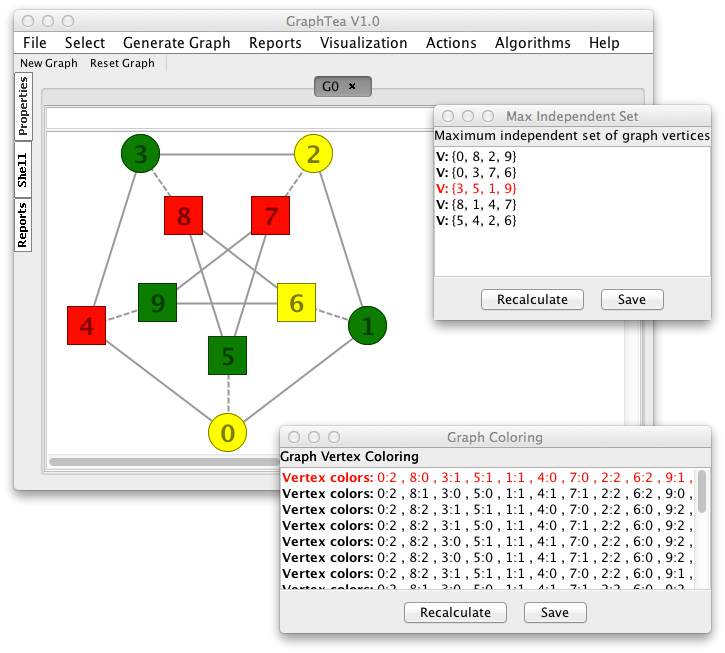
\includegraphics[width=0.7\textwidth]{graphtea}
\caption{An overview of GraphTea: A graph drawing window and
two floating dialogs with reports on a given graph.}
\label{f.graphtea}
\end{figure}
%-----------------------------------------------------------------------------------------------

Beside the automatic generation of graphs up to any size, we added the ability of loading
different sparse matrix as graphs to GraphTea.
A new data structure for the sparse matrix, called \textit{SpMat}, is designed
to handle the large sparse matrices. This data structure is basically an array.
This array has the size of number of rows. Each cell of this array points to
an array which is the corresponding columns of nonzeros in this row.

\textbf{MATLAB interface.}
%%%%%%%%%%%%%%%%%%%%%%%%%%%%%%%%%%%%%%%%%%%%%%%%%%%%%%%%%%%%%%%%%%%%%%%%%%%%%%%%%%%%%
\chapter{Interactive Educational Module}
\label{explain}
%%%%%%%%%%%%%%%%%%%%%%%%%%%%%%%%%%%%%%%%%%%%%%%%%%%%%%%%%%%%%%%%%%%%%%%%%%%%%%%%%%%%%
We develop an extensible collection of educational modules (\mbox{EXPLAIN})
to teach combinatorial scientific computing in classroom.
There is an increasing need for such educational tools since the connection
between the problem from scientific computing and the corresponding combinatorial
problem is tricky for the students.

\mbox{EXPLAIN} has two releases 1.0 and 2.0 so far which we will explain in more 
details in \secref{s.impl.explain}. Some of the modules which will be explained
are only available in the new release because of the efficiency. Both releases
are available now since they were developed on different technologies and have
pros and cons. However, the release 2.0 is an improved version and is developed
regularly.

During this chapter, we look first at the conceptual design of the software in
\secref{s.concept}. Then, we apply the gamification ideas on the software in
\secref{s.game} to involve the students more into the usage of \mbox{EXPLAIN}.
We explain how the conceptual design is finally visualized in \secref{s.vis}.
After looking at the available modules in \secref{s.av.modules}, we look at 
some implementation details in \secref{s.impl.explain}.
%%%%%%%%%%%%%%%%%%%%%%%%%%%%%%%%%%%%%%%%%%%%%%%%%%%%%%%%%%%%%%%%%%%%%%%%%%%%%%%%%%%%%
\section{Conceptual Design}
\label{s.concept}
%%%%%%%%%%%%%%%%%%%%%%%%%%%%%%%%%%%%%%%%%%%%%%%%%%%%%%%%%%%%%%%%%%%%%%%%%%%%%%%%%%%%%
Throughout the design stage, we were focused on the following goals.
This software is a self-study tool and the connection between the scientific computing
and combinatorial problems are explained by teacher in classroom.
The students can follow the algorithm on the graph by either
clicking on the vertices or edges.
So, neither the matrix nor its nonzeros are not clickable.
Clicking results in the modifications in both graph and matrix.
The available modifications on graph and matrix can be one or more actions
from the following list,
\begin{itemize}
\item Removing, adding, or coloring a vertex
\item Removing, adding, or coloring an edge
\item Changing the positions of vertices
\item Permutating matrix columns or rows or both.
\item Coloring any cell, column, or row of matrix
\end{itemize}

A sparse matrix is given as an input and the corresponding graph is built from this matrix.
The matrix and the corresponding graph are visualized side by side.
The graph model can be from one of the following types,
\begin{itemize}
\item Simple graph: an undirected graph without self-loops considering the given matrix as an adjacency matrix of graph.
\item Column-intersection graph: the graph explained in \defref{d:cig}.
\item Directed graph: the directed graph modle explained in \cite{Gebremedhin05whatcolor}.
\item Bipartite graph: the bipartite graph model explained in \defref{d.bip.graph}.
\end{itemize}

We define a set of predefined list of colors which can be selected by
the corresponding numbers, for example
$\{1=\text{green}, 2=\text{turquoise}, 3=\text{orange}, 4=\text{violet},
5=\text{red}, 6=\text{yellow}, ...\}$.
There colors are selected such that they look perceptually distinct.
However, a user can define any new color by \textbf{rgb} function.

%%%%%%%%%%%%%%%%%%%%%%%%%%%%%%%%%%%%%%%%%%%%%%%%%%%%%%%%%%%%%%%%%%%%%%%%%%%%%%%%%%%%%
\section{Gamification}
\label{s.game}
%%%%%%%%%%%%%%%%%%%%%%%%%%%%%%%%%%%%%%%%%%%%%%%%%%%%%%%%%%%%%%%%%%%%%%%%%%%%%%%%%%%%%
Though our primary aim is to design an educational model for illustrating the connection between
scientific computing and graph theory, we also experience with ideas from gamification
\cite{deterding2011:gug,deterding2011}. The use of elements from game design in the context of
computer science education is not new. In particular, programming assignments can involve
implementations of games. In \cite{la2007:gfa}, for instance, an introductory programming course is
taught under the common umbrella of two-dimensional game development. Similarly, a game project is
used in a course on software architecture~\cite{Wang2011:EEU}. Programming assignment can also
involve pieces of software that act as a player in an existing game. However, throughout the
present paper, our focus of serious games is different. Rather than implementing a game, we are
interested in situations where students learn by playing a game. Surprisingly, there are only a few
publications addressing this aspect of gamification. An example is given in
\cite{Hakulinen2011:usg} where game-based learning is used to teach a course in data structures and
algorithms. A collaborative game is described in \cite{shl:bsc} that aims at improving the teaching
quality of a course on mathematical logic.

To engage the students more in the teaching process, we improved EXPLAIN such that the students get
more feedback from the software. Gamification of the software does this by interpreting each
solution to a problem instance as a \textit{round}. The score diagram reporting the results of previous
rounds also provides another feedback. The idea of gamification is used to solve a combinatorial
minimization problem consisting of minimizing the size of the vertex separator while, at the same
time, balancing the size of the remaining components. The consistent use of colors in the graph
view, the matrix view, and in the score diagram makes it easier for the student to understand
minimizing a serial bottleneck in the Cholesky factorization while balancing the computational
load.
%%%%%%%%%%%%%%%%%%%%%%%%%%%%%%%%%%%%%%%%%%%%%%%%%%%%%%%%%%%%%%%%%%%%%%%%%%%%%%%%%%%%%%
\section{Visualization}
\label{s.vis}
Based on our goal to visualized the connection of the algorithm on the matrix and graph sides simultaneously,
we designed the software to have the four sections as illustrated in \figref{explain-design} (Left).
The graph is drawn on the circular layout first. The layout can be selected later
in the control panel. The matrix is visualized also at the right side and
their nonzero elements are shown by the notation $\times$.
\figref{explain-design} (Right) shows an actual example of the implemented view of
\mbox{EXPLAIN}.

%%%%%%%%%%%%%%%%%%%%%%%%%%%%%%%%%%%%%%%%%%%%%%%%%%%%%%%%%%%%%%%%%%%%%%%%%%%%%%%%%%%%%%
\begin{figure}
\centering
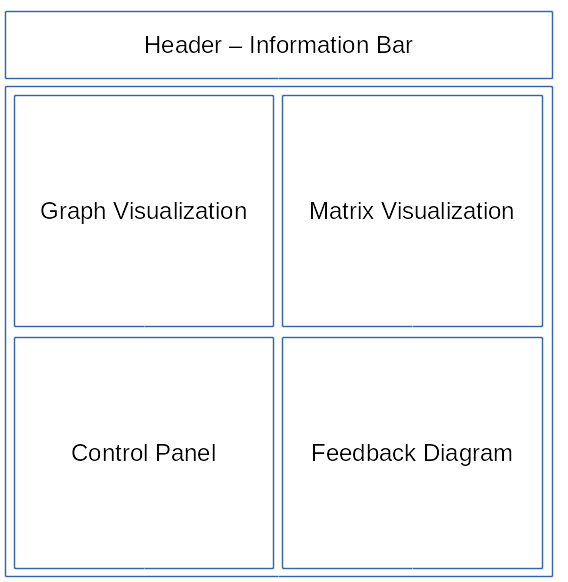
\includegraphics[width=0.44\textwidth]{explain-vis.png}
\hfill
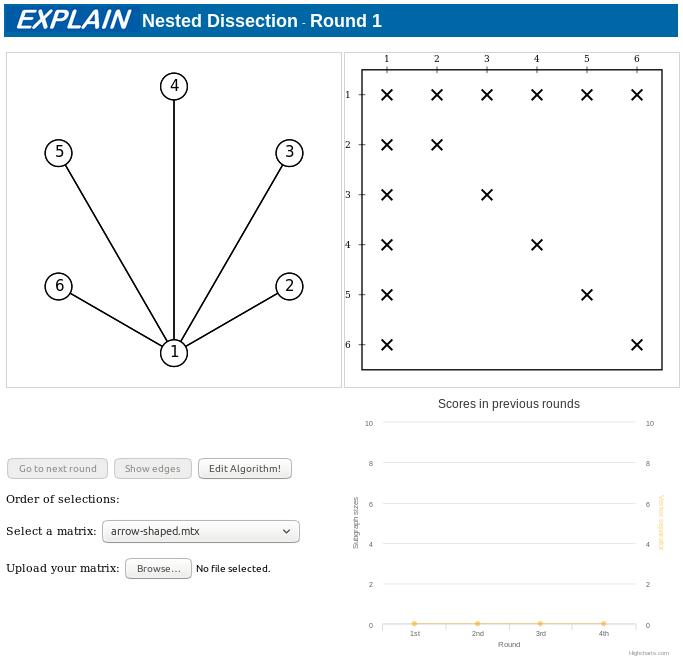
\includegraphics[width=0.48\textwidth]{explain2-init.png}
\caption{
(Left)~\mbox{EXPLAIN} has a fixed layout consists of four sections and a header.
(Right)~An example of the actual implemented view of \mbox{EXPLAIN}.}
\label{explain-design}
\end{figure}
%%%%%%%%%%%%%%%%%%%%%%%%%%%%%%%%%%%%%%%%%%%%%%%%%%%%%%%%%%%%%%%%%%%%%%%%%%%%%%%%%%%%%
\section{Available Modules}
\label{s.av.modules}
%%%%%%%%%%%%%%%%%%%%%%%%%%%%%%%%%%%%%%%%%%%%%%%%%%%%%%%%%%%%%%%%%%%%%%%%%%%%%%%%%%%%%
%%%%%%%%%%%%%%%%%%%%%%%%%%%%%%%%%%%%%%%%%%%%%%%%%%%%%%%%%%%%%%%%%%%%%%%%%%%%%%%%%%%%%
\subsection{Column Compression}
\label{s.column-compression}
%%%%%%%%%%%%%%%%%%%%%%%%%%%%%%%%%%%%%%%%%%%%%%%%%%%%%%%%%%%%%%%%%%%%%%%%%%%%%%%%%%%%%
In \cite{2013:05,2014:01}, we presented an educational module in \mbox{EXPLAIN} to visualize the
coloring algorithm for the column compression interactively. The idea is
summarized as follows.

\begin{figure}
\centering
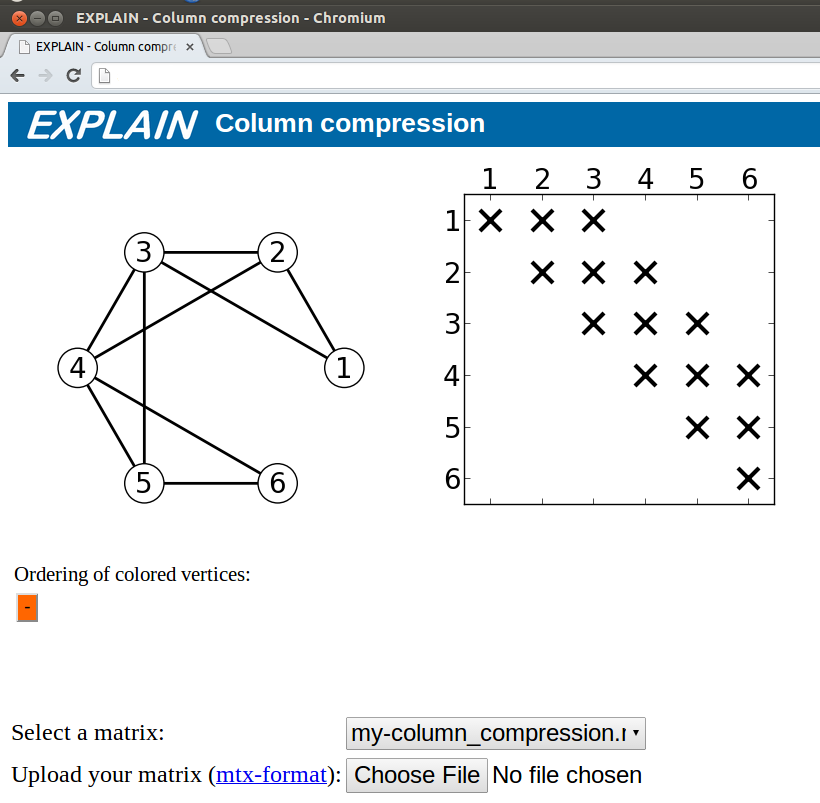
\includegraphics[width=0.5\textwidth]{fig1.png}
\caption{The initial layout of EXPLAIN for some given column compression problem. Matrix and graph are visualized side by side to recognize the underlying connection between these two equivalent representations. Nonzero elements are indicated by the symbol $\times$.}
\label{fig1}
\end{figure}
The module allows to select and, thus, color the vertices of a given graph step by step. The order in which the vertices are colored is interactively selected by the student. In each step, when the student selects a vertex, the program checks all of its neighbors regarding the colors. A color of the current step is then greedily selected from a predefined list, $\{1=\text{green}, 2=\text{turquoise}, 3=\text{orange}, 4=\text{violet}, 5=\text{red}, 6=\text{yellow}, ...\}$, such that it differs from the colors of those neighbors that are already colored. Recall that a group of columns corresponds to a set of vertices in the graph with the same color. To indicate this, we do not color only the vertices in the graph but also the corresponding columns in the matrix.

\figurename~\ref{fig1} shows a screenshot of the column compression module. The nonzero elements of the matrix are denoted by the symbol $\times$ in the matrix view; the corresponding column intersection graph is given immediately next to the matrix. In the bottom of the page, different preloaded matrices can be selected or a new matrix can be uploaded from a file on the file system of the student's computer. The tool provides an interactive interface for the student who can control the algorithm such as returning to previous steps or loading different graphs and matrices. Selecting the vertices in different orderings generates different colorings corresponding to different column compressions.

Suppose a vertex is selected in the first step. This vertex is then colored using the first color of the predefined list. Continuing this process of vertex selection, different colors are chosen and an ordered list of vertices is created which is already indicated in \figurename~\ref{fig1} marked by ''Ordering of colored vertices.'' In this figure the list is empty but it will become non-empty in later figures. Each button of this list is clickable, causing \mbox{EXPLAIN} to return to that step of the algorithm. The process is continued until all vertices are colored. The button labeled by the minus sign will go back to the first step keeping the whole process history.


\begin{figure}
\centering
\subfigure[Student selected $v_2$ and $v_6$ in that order.]{
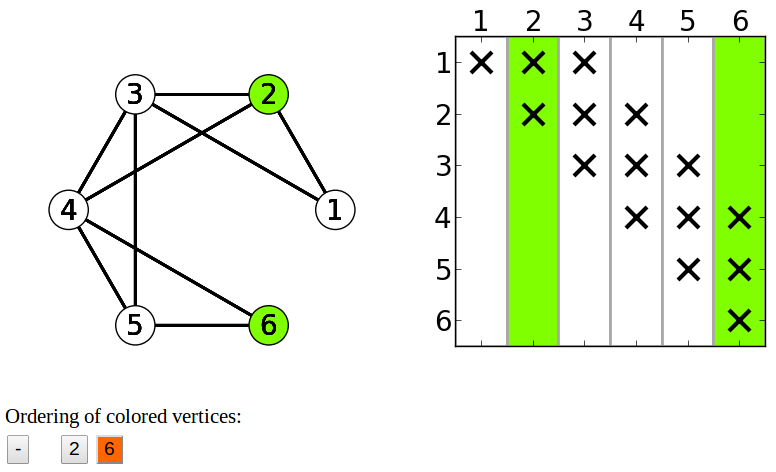
\includegraphics[width=0.47\textwidth]{fig2.png}
\label{fig2}
}
\centering
\subfigure[Student selected $v_2$, $v_6$, $v_3$, $v_5$, $v_1$, and $v_4$ in that order.]{
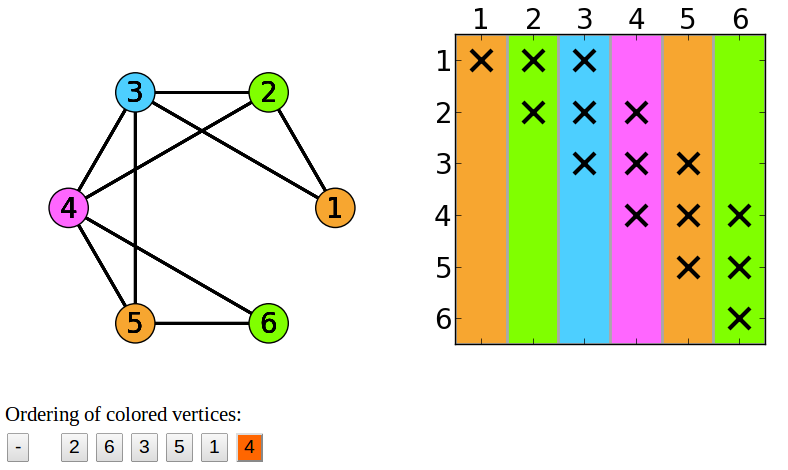
\includegraphics[width=0.47\textwidth]{fig3.png}
\label{fig3}
}
\centering
\subfigure[Student selected vertices as in \figurename~\protect\ref{fig3} and then jumped back to $v_2$.]{
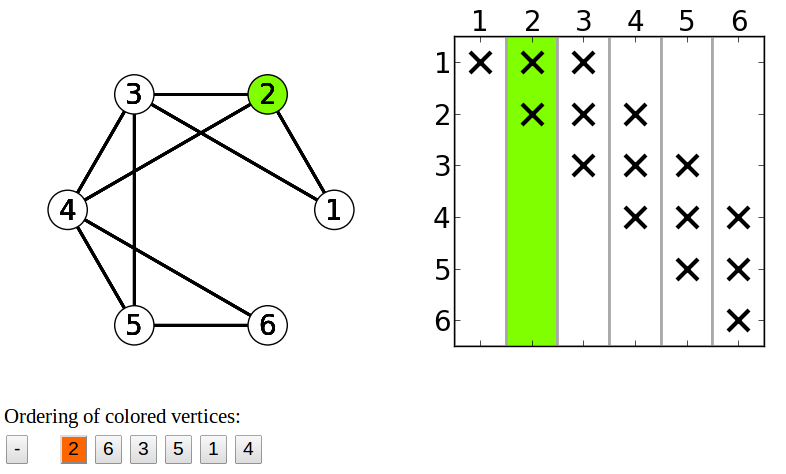
\includegraphics[width=0.47\textwidth]{fig4.png}
\label{fig4}
}
\centering
\subfigure[Student selected $v_2$, $v_1$, $v_3$, $v_4$, $v_5$, and $v_6$ in that order.]{
\includegraphics[width=0.47\textwidth]{fig5.png}
\label{fig5}
}
\caption{Display of various situations after interactively choosing vertices.}
\label{algorihtm}
\end{figure}
\figurename~\ref{fig2} shows a representation of nonzero pattern of the possible following matrix
\begin{equation}
\label{e:matrixJ}
J =
\begin{bmatrix}
1 & 2 & 3 & 0 & 0 & 0 \\
0 & 4 & 5 & 6 & 0 & 0 \\
0 & 0 & 7 & 8 & 9 & 0\\
0 & 0 & 0 & 10 & 11 & 12\\
0 & 0 & 0 & 0 & 13 & 14 \\
0 & 0 & 0 & 0 & 0 & 15
\end{bmatrix},
\end{equation}

and the related graph in which the student has already selected the two vertices $v_2$ and $v_6$. \figurename~\ref{fig3} represents the final step which shows that four colors are needed when the vertices are selected in the order $(v_2, v_6, v_3, v_5, v_1, v_4)$ displayed in the vertex list. The group of columns with the same color is compressed to a single column in the seed matrix as follows,
\begin{equation}
\label{e:matrixS}
J \cdot S =
J \cdot
\begin{bmatrix}
0 & 0 & 1 & 0 \\
0 & 1 & 0 & 0 \\
0 & 0 & 0 & 1 \\
0 & 0 & 1 & 0 \\
1 & 0 & 0 & 0
\end{bmatrix}
=
\begin{bmatrix}
2 & 3 & 1 & 0 \\
4 & 5 & 0 & 6 \\
0 & 7 & 9 & 8 \\
12 & 0 & 11 & 10\\
14 & 0 & 13 & 0 \\
15 & 0 & 0 & 0
\end{bmatrix}.
\end{equation}
Furthermore, the coloring of \figurename~\ref{fig3} is exactly the one corresponding to that compressed Jacobian~\eqref{e:matrixS}.

Since we want to provide the possibility to return to some step of the algorithm, a history of the selection process is kept in the ordered vertex list. Now, suppose the student selects to return to the step $1$ where the vertex $v_2$ was selected, then the program returns to that step of the algorithm. The resulting state is depicted in \figurename~\ref{fig4}. Notice that the program keeps the whole history and the student can click on any other vertex in the history.

On the other hand, the student can select a completely new selection order from the current step which can generate a smaller or larger number of colors. Employing the different ordering $(v_2,v_1,v_3,v_4,v_5,v_6)$ shown in \figurename~\ref{fig5} leads to a reduction of one color compared to the first ordering given in \figurename~\ref{fig3}. Actually, this is the minimum number of colors needed to color this graph. The corresponding seed matrix is given by
$$
S =
\begin{pmatrix}
1 & 0 & 0 \\
0 & 1 & 0 \\
0 & 0 & 1 \\
1 & 0 & 0 \\
0 & 1 & 0 \\
0 & 0 & 1 \\
\end{pmatrix}.
$$
%%%%%%%%%%%%%%%%%%%%%%%%%%%%%%%%%%%%%%%%%%%%%%%%%%%%%%%%%%%%%%%%%%%%%%%%%%%%%%%%%%%%%
\subsection{Bidirectional Compression}
\label{s.bidirectional}
%%%%%%%%%%%%%%%%%%%%%%%%%%%%%%%%%%%%%%%%%%%%%%%%%%%%%%%%%%%%%%%%%%%%%%%%%%%%%%%%%%%%%
In our publication~\cite{2014:09}, we design and implement an interactive module to
teach bidirectional compression and its connection to star bicoloring.
Figure~\ref{f.explain} shows an overview of the layout of the new module whose top and
bottom part are shown in~(a) and~(b), respectively. In the top part, a graph and a matrix
are visualized next to each other. Here, a matrix with a sparsity pattern in the form of
an arrow is taken as an example. The nonzero pattern of the matrix is shown right and the
corresponding bipartite graph is depicted left. A vertex $r_i$, which is placed on the
left part of the graph, represents the $i$th row of the matrix. Likewise, a vertex on the
right part of the graph labeled $c_i$ corresponds to the $i$th column of the matrix.
Different matrices can be selected from a predefined list or can be uploaded to the
server using the menu depicted in Fig.~\ref{f.explain} (b). We stress that EXPLAIN is
designed for small problem instances.

%------------------------------------------------------------------------------------------------
\begin{figure}
\centering
\subfigure[]{\includegraphics[width=0.43\textwidth]{init-bipartite}}
\hfill
\subfigure[]{\includegraphics[width=0.55\textwidth]{explain_bottom}}
\caption{The general layout of the bidirectional compression module. (a) The top part
contains the visualization of the graph and its corresponding matrix. (b)
The bottom part contains the intermediate steps, the input, and the
history of selections.}
\label{f.explain}
\end{figure}
%------------------------------------------------------------------------------------------------


%------------------------------------------------------------------------------------------------
\begin{figure}
\centering
\subfigure[]{%
% Matrix C: after choosing 2 vertices
\includegraphics[width=0.18\textwidth]{arrow-shaped-bipartite-graph-twoselected}
\includegraphics[width=0.24\textwidth]{arrow-shaped-matrix-twoselected}
}
\hfill
\subfigure[]{%
% Matrix C: after having completed the solution process
\includegraphics[width=0.18\textwidth]{arrow-shaped-almost-worst-coloring-graph}
\includegraphics[width=0.24\textwidth]{arrow-shaped-almost-worst-coloring-matrix}
}%
\caption{The graph and the nonzero pattern (a) taken from Fig.~\protect\ref{f.explain}
after the student interactively selected the vertices $r_2$
and $c_1$. A star bicoloring (b) of that example after trying to solve
\MinStaBic\ interactively. This star bicoloring uses $11$ colors.}
\label{f.arrow-shaped2}
\end{figure}
%------------------------------------------------------------------------------------------------

Using any web browser, the student can interactively solve \MinStaBic\ by clicking on
vertices of the bipartite graph. The selection of a vertex by a click refers to choosing
this vertex to be colored next. This coloring is visualized simultaneously in the graph
as well as in the matrix where the neutral color is the color white. By clicking on a row
vertex, the vertex itself and the corresponding row is colored. This color should obey
the rules specified in the definition of a star bicoloring. By clicking on a column
vertex, this vertex and the corresponding column are colored. Recall that a nonzero
element may be in both a colored column as well as in a colored row. In this case, we
divide the square surrounding this element into a triangle and the remaining part. The
triangle part is colored with the row color and the remaining part of the rectangle with
the column color.

%------------------------------------------------------------------------------------------------
\begin{figure}
\centering
\subfigure[]{%
% Matrix C: Minimal number of colors
\includegraphics[width=0.18\textwidth]{arrow-shaped-best-coloring-graph}
\includegraphics[width=0.24\textwidth]{arrowshaped-best-coloring-matrix}
}%
\hfill
\subfigure[]{%
% A different matrix : after having completed the solution process
\includegraphics[width=0.18\textwidth]{arrow-shaped2-best-coloring-graph}
\includegraphics[width=0.24\textwidth]{arrow-shaped2-best-coloring-matrix}
}%
\caption{A star bicoloring (a) of the problem instance from
Fig.~\protect\ref{f.explain} also considered in Fig.~\protect\ref{f.arrow-shaped2}. This
star bicoloring uses $3$ colors and is an exact solution of \MinStaBic. A star bicoloring
(b) of a different problem instance using $4$ colors which is also an exact
solution of \MinStaBic} \label{f.arrow-shaped4}
\end{figure}
%------------------------------------------------------------------------------------------------

We now take the problem with the arrow-shaped nonzero pattern from Fig.~\ref{f.explain}
as an example. Here and in the following, we zoom into the graph and matrix view of the
layout. The student interactively selects a sequence of row and column vertices to solve
\MinStaBic. Figure \ref{f.arrow-shaped2} (a) shows the situation after the student
selected the vertices $r_2$ and $c_1$.

The interactive selection then goes back and forth until a correct star bicoloring is
found. In EXPLAIN, the process of computing a solution of \MinStaBic\ is called a round.
The current round number is displayed at the top of the web page; see
Fig.~\ref{f.explain}~(a). When a coloring is found at round number $x$, the page shows
the message ``Round $x$ is completed!''

Selecting vertices in different orders will typically result in different star
bicolorings. A star bicoloring which is interactively chosen will not always have a
minimal number of colors. For example, the order of vertex selection visualized in
Fig.~\ref{f.arrow-shaped2}~(b) leads to a star bicoloring using $11$ colors, which is
obviously not the minimal number of colors. Here, all columns and rows are colored
differently. In contrast, Fig.~\ref{f.arrow-shaped4}~(a) illustrates an exact solution of
\MinStaBic\ for this problem instance using the minimal number of $3$ colors.

After completing a round, the student can solve the same problem instance once more. In
this case, the round number will be incremented, the colors will be removed, and another
round is started using the initial situation depicted in Fig.~\ref{f.explain}~(a). The
history of the number of non-neutral colors used in previous rounds is displayed below
the matrix in a score diagram as shown in Fig~\ref{f.explain}~(b). The idea behind this
score diagram is to use elements of game design to motivate and increase the student's
activity in the learning process. This way, the student can see how successful he or she
was in reducing the number of non-neutral colors.

The subtle issues in understanding the connection between bidirectional compression and
star bicoloring are more lucid when considering more irregularly-structured nonzero
patterns. Another problem instance with a different nonzero pattern is shown in
Fig.~\ref{f.arrow-shaped4}~(b). Here, it is more difficult to find out that this star
bicoloring with $4$ colors is indeed an exact solution to \MinStaBic.

\subsection{Partial Jacobian Computation}
The previous module of matrix compression is extended to support
also the partial Jacobian computation. Here, the student should
first select the required elements which are edges in Bipartite graphs.
So, when the student clicks on the edges, the colors of those edges change to red
and the corresponding nonzero elements are added to required elements.

As soon as the student starts to click the vertices, the required elements
are become fixed, i.e. no new required elements can be added.
The other processes of coloring are completely like the previous module.


%------------------------------------------------------------------------------------------------
\begin{figure}
\centering
\subfigure[]{%
% Matrix C: Minimal number of colors
\includegraphics[width=0.18\textwidth]{arrow-shaped-best-coloring-graph}
\includegraphics[width=0.24\textwidth]{arrowshaped-best-coloring-matrix}
}%
\hfill
\subfigure[]{%
% A different matrix : after having completed the solution process
\includegraphics[width=0.18\textwidth]{arrow-shaped2-best-coloring-graph}
\includegraphics[width=0.24\textwidth]{arrow-shaped2-best-coloring-matrix}
}%
\caption{A star bicoloring (a) of the problem instance from
Fig.~\protect\ref{f.explain} also considered in Fig.~\protect\ref{f.arrow-shaped2}. This
star bicoloring uses $3$ colors and is an exact solution of \MinStaBic. A star bicoloring
(b) of a different problem instance using $4$ colors which is also an exact
solution of \MinStaBic} \label{f.arrow-shaped4}
\end{figure}
%------------------------------------------------------------------------------------------------

\subsection{Nested Dissection Ordering}
Given a sparse symmetric matrix $A$, the nested dissection method finds a 
symmetric permutation $P^T A P$ of $A$ 
such that the permutated matrix gets the following form,
$$
A^{\prime} =
\begin{bmatrix}
A_1 & 0   & \cdots & 0 & B_1^T \\
0   & A_2 & \cdots & 0  & B_2^T \\
\vdots& \vdots & \ddots & 0 & \vdots \\
0   &   0 & \cdots & A_p & B_p^T \\
B_1 & B_2 & \cdots & B_p& C
\end{bmatrix},
$$
in which the size of the block matrices $A_1,...,A_p$ are balanced, 
and the size of block $C$ is minimum.
This reduces the computational work in different application areas.
An example can be found in \cite{2014:02}.

The graph model of this problem has the simple graph layout considering the matrix
as the adjacency matrix of a graph. 
The algorithm from~\cite{2014:02} searches for a so-called vertex-separator set
corresponding to the block $C$ here. A vertex separator $S$ of the given graph $G$ 
is a subgraph of $G$ if removing $S$ and its adjacent edges from $G$ results in two
disconnected components $V_1$ and $V_2$ of $G$. 
Suppose we move rows and columns corresponding to the vertex separator to the end of
the matrix and bringing together 
the corresponding columns of $V_1$ and $V_2$ by a permutation,
then a nested dissection would be visualized on the matrix.

We extended \mbox{EXPLAIN} with
a new module that considers the nested dissection ordering
of a given matrix and the equivalent graph problem, i.e.,
finding a vertex separator (see~\cite{2014:02} for the bisection). 
In this module, a round consists of finding a vertex separator.
We look first at a bisection, i.e. $p=2$. 
Figure~\ref{initial_10} shows the initial layout of an example 
and the selection of the vertex $10$ for the set of vertex separator. The module moves the 
corresponding column to the selected vertex to the end of the matrix
and both the vertex and its corresponding column get the orange color.
Additionally, the adjacent edges of the vertex are removed for a better visualization.

\begin{figure}
\centering
\subfigure[]{
\includegraphics[width=0.23\textwidth]{graph_initial}
\includegraphics[width=0.23\textwidth]{matrix_initial}}
\hfill
\subfigure[]{
\includegraphics[width=0.23\textwidth]{graph_10_selected}
\includegraphics[width=0.23\textwidth]{matrix_10_selected}}
\caption{
(a) Two equivalent representations in terms of a graph and a matrix.
(b) Graph and matrix view after selecting the vertex number~10.
The decomposition into two blocks is still not shown as the graph is not yet
decomposed into two disconnected components.}
\label{initial_10}
\end{figure}

Figure~\ref{selected_4_10_8_10} shows two scenario of selection with 
the worst and best case of selection. The left selection~\figref{selected_4_10_8_10}(a)
in which the vertex
$4$ is selected after the initial selection of $10$, we have an unbalanced result.
However, the right selection~\figref{selected_4_10_8_10}(b) results in a balanced result
by only selecting $8$ instead of $4$. 
When a vertex separator is found, the software colors the two disconnected components of graph
as well as the distinct block on diagonals after permutation
with blue and red.

\begin{figure}
\centering
\subfigure[]{
\label{selected410}
\includegraphics[width=0.23\textwidth]{graph_4_10_selected}
\includegraphics[width=0.23\textwidth]{matrix_4_10_selected}}
\hfill
\subfigure[]{
\label{selected810}
\includegraphics[width=0.23\textwidth]{graph_8_10_selected}
\includegraphics[width=0.23\textwidth]{matrix_8_10_selected}}
\caption{
(a) Graph and matrix view after selecting the vertices number 10 and then 4.
The selection is not adequate as the sizes of blocks are not balanced.
(b) Graph and matrix view after selecting the vertices number 10 and then 8. The block sizes are balanced and the separator size is minimized.}
\label{selected_4_10_8_10}
\end{figure}

A resulting score diagram from different rounds looks
like \figref{diagram}. Here, the blue and red curves should have
values close to each other since this indicates the balancing condition.
The orange curve should be as low as possible
because it represents the minimization of the separator size.
In this figure, the separator size is indeed minimal and the
balance condition is satisfied in the last round.
\begin{figure}
\centering
\includegraphics[width=0.47\textwidth]{diagram}
\caption{Score diagram resulting from four different rounds.}
\label{diagram}
\end{figure}

Based on the new features of \mbox{EXPLAIN 2.0}, we could improved the previous
bisection to a recursive nested dissection algorithm.
It contains the bisection itself. So, the student selects the vertex separator
as before until the graph becomes disconnected.
In this new version, the vertex separator will be shown on the bottom
of the graph. Also the two remaining parts of graph are shown separately
in two different circles at right and left.
In Figure~\ref{bad_bisection}, the result of a selection is visualized which
is inefficient since the parts of graphs are not balanced.
Figure~\ref{good_bisection} also shows the results of an efficient selection.

\begin{figure}
\centering
\includegraphics[width=0.8\textwidth]{bad_bisection}
\caption{A selection results in an inefficient bisection of graph.}
\label{bad_bisection}
\end{figure}

\begin{figure}
\centering
\includegraphics[width=0.8\textwidth]{good_bisection}
\caption{A selection results in an efficient bisection of graph.}
\label{good_bisection}
\end{figure}

\begin{figure}
\centering
\includegraphics[width=0.8\textwidth]{bad_disection}
\caption{A complete nested dissection up to the order 2 which has an
inefficient result.}
\label{bad_disection}
\end{figure}


\begin{figure}
\centering
\includegraphics[width=0.8\textwidth]{good_disection}
\caption{A complete nested dissection up to the order 2 which has an
efficient result.}
\label{good_disection}
\end{figure}

\begin{figure}
\centering
\includegraphics[width=0.8\textwidth]{good_disection2}
\caption{A complete nested dissection up to the order 2 which has an
even more efficient result.}
\label{good_disection2}
\end{figure}

Now, in contrast to the previous version, the student can click further
on the vertices of each part. This selection would trigger a recursive
bisection of the matrix as well. Again, this selection goes forward until
both parts of the graphs become disconnected. The vertex separators
would be moved to the bottom of the graph parts as well as the graph parts
would be shown separately. Figure~\ref{bad_disection} and Figure~\ref{good_disection} illustrated two inefficient and efficient results of nested dissection,
respectively. Figure~\ref{good_disection2} shows how the results can
get even better by a suitable order of selection.

The corresponding diagram of the history of rounds is improved such that
both the size of vertex separator as well as the size of four graph parts
can be visualized. Figure~\ref{barchart} shows a possible selection history.
As it can be seen the line chart shows the size history of the vertex separator
and four bar chart grouped together shows the size history of the graph parts.
The colors are also the same colors which are used in the graph and matrix visualizations.
Since the goal here is to minimize the size of vertex separator as well as balancing the 
size of subgraphs, we achieved the optimum results in the fourth round of selection.
\begin{figure}
\centering
\includegraphics[width=0.6\textwidth]{chart2}
\caption{The size of four subgraphs, shown as bar charts,
resulted from nested dissection compared in different rounds.
The color of bar charts are related to the colors of corresponding subgraph.
The curve of the orange color is also the size of vertex separator.}
\label{barchart}
\end{figure}

\subsection{Parallel Matrix Vector Product}

In \cite{2015:3}, we extended EXPLAIN with a new module for
the parallel sparse matrix-vector multiplication.
So if we show the problem as follows,
$$
\vek{y} = \mat{A}\cdot \vek{x}
$$
or by elements as follows,
\begin{equation}
\label{e.yax}
\vek{y} \leftarrow \mat{A} \vek{x}
\end{equation}
where the $N$-dimensional vector $\vek{y}$ is the result of applying \mat{A} to some
given $N$-dimen\-sional vector $\vek{x}$. Then, the $i$th entry of~$\vek{y}$ is given by
\begin{equation}
\label{e.mvp}
y_i = \sum_{j \text{ with } a_{ij} \neq 0} a_{ij} \cdot x_j ,
\quad
i = 1, 2, \dots, N,
\end{equation}
The question here is if data representing \mat{A}, \vek{x} and
\vek{y} are distributed to multiple processes, to what extent does this data distribution
have an effect on the computation $\vek{y} \leftarrow \mat{A} \vek{x}$? What are the
advantages and disadvantages of a given data distribution? What are the criteria for
evaluating the quality of a data distribution? How should data be distributed to the
processes ideally?


To discuss such questions with undergraduates who are new to parallel computing we
suggest to consider the following simple data distribution. The nonzero elements
of~\mat{A} are distributed to processes by rows. More precisely, all nonzeros of a row
are distributed to the same process. The vectors \vek{x} and \vek{y} are distributed
consistently. That is, if a process stores the nonzeros of row $i$ of~\mat{A} then it
also stores the vector entries~$x_i$ and~$y_i$. Given a fixed number of processes $p$, a
data distribution may be formally expressed by a mapping called \emph{partition}
$$
P: I \rightarrow \{1, 2, \dots, p\}
$$
that decomposes the set of indices $I := \{1, 2, \dots, N\}$ into~$p$ subsets $I_1$,
$I_2$, \dots, $I_p$ such that
$$
I = I_1 \cup I_2 \cup \dots \cup I_p
$$
with $I_i \cap I_j = \emptyset$ for~$i \neq j$. That is, if $P(i)=k$ then the nonzeros of
row~$i$ as well as~$x_i$ and~$y_i$ are stored on process $k$.

Since the nonzero $a_{ij}$ is stored on process~$P(i)$ and the vector entry~$x_j$ is
stored on process~$P(j)$, one can sort the terms of \eqref{e.mvp} according to
those terms where both operands of the product $a_{ij} \cdot x_j$ are stored on the same
process and those where these operands are stored on different processes:
\begin{equation}
\label{e.pmvp}
y_i =
\sum_{ \substack{j \text{ with } a_{ij} \neq 0\\ P(i)=P(j)}} a_{ij} \cdot x_j
+ \sum_{ \substack{j \text{ with } a_{ij} \neq 0\\ P(i)\neq P(j)}} a_{ij} \cdot x_j ,
\quad i = 1, 2, \dots, N.
\end{equation}
For the sake of simplicity, we assume that the product $a_{ij} \cdot x_j$ is computed by
the process~$P(i)$ that stores the result $y_i$ to which this product contributes.
By~\eqref{e.pmvp}, the data distribution $P$ has an effect on the amount of data that
needs to be communicated between processes. It also determines which processes
communicate with each other. Since, on today's computing systems, communication needs
significantly more time than computation, it is important to find a data distribution
using a goal-oriented approach. A data distribution is desirable that balances the
computational load evenly among the processes while, at the same time, minimizes the
communication among the processes.

The problem of finding a data distribution is also interesting from another perspective
of undergraduate teaching. It offers the opportunity to demonstrate that a theoretical
model can serve as a successful abstraction of a practical problem. More precisely, a
formal approach using concepts from graph theory is capable of tackling the data
distribution problem systematically.

To this end, we now assume that the nonzero pattern of the asymmetric matrix \mat{A} is
symmetric. Then, the matrix can be represented by an undirected graph $G=(V,E)$. The set
of nodes $V = \{ 1, 2, \dots, N\}$ is used to associate a node to every row (or
corresponding column) of \mat{A}. The set of edges
\begin{displaymath}
E = \{ (i,j) \mid i, j \in V \text{ and } a_{ij} \neq 0 \text{ for } i > j \}
\end{displaymath}
describes the nonzero entries. Here, the condition $i>j$ indicates that the edge~$(i,j)$
is identical to the edge~$(j,i)$ and that there is no self-loop in $G$. The data
distribution to $p$ processes is then represented by the partition
$$
P: V \rightarrow \{1, 2, \dots, p\}
$$
that decomposes the set of nodes $V$ of the graph into~$p$ subsets $V_1$, $V_2$, \dots,
$V_p$ such that
$$
V = V_1 \cup V_2 \cup \dots \cup V_p
$$
with $V_i \cap V_j = \emptyset$ for~$i \neq j$.


Then, \eqref{e.mvp} is reformulated in terms of graph terminology by
\begin{displaymath}
y_i = a_{ii} \cdot x_i +
\sum_{ \substack{(i,j)\in E \\ P(i)=P(j)}} a_{ij} \cdot x_j
+ \sum_{ \substack{(i,j)\in E \\ P(i)\neq P(j)}} a_{ij} \cdot x_j .
\end{displaymath}
Here, the first two terms of the right-hand side can be computed on process~$P(i)$
without communication to any other process. The condition~$P(i)\neq P(j)$ in the last
term shows that the computation of $a_{ij} \cdot x_j$ requires communication between
process~$P(i)$ which stores~$a_{ij}$ and process~$P(j)$ which stores $x_j$. Minimizing
interprocess communication then roughly corresponds to minimizing the number of edges
connecting nodes in different subsets~$V_i$ of the partition $P$. This number of edges is
called the \emph{cut size} and is formally defined by
\begin{equation}\label{e.cut}
\operatorname{cutsize}(P) = \bigl| \{ (i,j) \in E \mid P(i)\neq P(j) \} \bigr|.
\end{equation}
In this graph model, the cut size does not exactly correspond to the number of words
communicated between all processes in the computation of $\vek{y} \leftarrow \mat{A}
\vek{x}$ for a given partition $P$. However, it gives a reasonable approximation to this
amount of communicated data called the \emph{communication volume}; see the corresponding
discussion in~\cite{hk:mod}. The communication volume is exactly described by the cut
size if the underlying model is changed from an undirected graph to a
hypergraph~\cite{ca:hyp,cua:hyp,ua:rev}.

Assuming that the number of nonzeros is roughly the same for each row of~\mat{A}, the
computation is evenly balanced among the $p$ processes if the partition $P$ is
$\varepsilon$-balanced defined as
\begin{equation}\label{e.bal}
\max_{1 \leq i \leq p} |V_i| \leq (1 + \varepsilon) \frac{|V|}{p} ,
\end{equation}
for some given $\varepsilon > 0$. The graph partitioning problem consists of minimizing
the cut size of an $\varepsilon$-balanced partition. It is a hard combinatorial
problem~\cite{gj:com}.


To illustrate the connection between computing a sparse matrix-vector multiplication in
parallel and partitioning an undirected graph, we propose a novel educational module.
This module is part of a growing set of educational modules called EXPLoring Algorithms
INteractively (EXPLAIN). This collection of web-based modules is designed to assist in
the effectiveness of teachers in the classroom and we plan to make it publicly available
shortly. Figure~\ref{f.explain.matvec} shows the overall layout of this interactive
module for sparse matrix-vector multiplication. The top of this figure visualizes---side by side---the representation of the problem regarding the graph~$G$ as well as in terms
of the matrix~\mat{A} and the vector \vek{x}. Below on the left, there is a panel of
colors representing different processes and another panel displaying the order of
selecting vertices of the graph. Next, on the right, there is a score diagram recording
values characterizing communication and load balancing. At the bottom part, there are
input controls used to select a matrix from a predefined set of matrices, to upload a
small matrix, and to choose the layout of the graph vertices.


%------------------------------------------------------------------------------------------
% Overall Layout of Module
\begin{figure}
\centering
\includegraphics[width=0.7\textwidth]{final}
\caption{Overall structure of the sparse matrix-vector multiplication module.}
\label{f.explain.matvec}
\end{figure}
%------------------------------------------------------------------------------------------

The first figure gives an overall impression of the status of the module after a data
distribution is completed. Here, $p=4$ processes represented by the colors blue, green,
red, and yellow get data by interactive actions taken by the student.
Figure~\ref{f.beginning} now shows the status of the module in a phase that is more
related to the beginning of that interactive procedure. For a given matrix, the student
can distribute the data to the processes by first clicking on a color and then clicking
on an arbitrary number of vertices. That is, the distribution of vertices to a single
process is determined by first clicking on a color $j$ and then clicking on a particular
number of vertices, say $i_1, i_2, \dots, i_s$ such that $P(i_1) = P(i_2) = \dots =
P(i_s) = j$. Then, by clicking on the next color, this procedure can be repeated until
all vertices are interactively colored and, thus, the data distribution $P$ is finally
determined.

Figure~\ref{f.beginning} illustrates the situation after the student distributed
vertices~1, 2 and 3 to the blue process and the vertices~7, 8 and 10 to the green
process. By interactively assigning a vertex to a process, not only the vertex is colored
by the color representing this process, but also the row in the matrix as well as the
corresponding vector entry of \vek{x} are simultaneously colored with the same color.
This way, the data distribution is visualized in the graph and in the matrix
simultaneously which emphasizes the connection between the matrix representation and the
graph representation of that problem. The panel labeled ``Order of selection'' records
the order of the vertices that are interactively chosen. By inspection from that panel
in~\figref{f.explain}, we find out that the status depicted in \figref{f.beginning} is an
intermediate step of the interactive session that led to the data distribution
in~\figref{f.explain}. Any box labeled with the number of the chosen vertex in that panel
is also clickable allowing the student to return to any intermediate state and start a
rearrangement of the data distribution form that state.


%------------------------------------------------------------------------------------------
% Interactive Selection of Vertices
\begin{figure}
\centering
\includegraphics[width=0.7\textwidth]{twoColors}
\caption{The intermediate state after the student selected six vertices.}
\label{f.beginning}
\end{figure}
%------------------------------------------------------------------------------------------

In EXPLAIN, the term ``round'' refers to the process of solving a single instance of a
given problem. In this module, the problem consists of distributing all data needed to
compute the matrix-vector product to the processes. Equivalently, the distribution of all
vertices of the corresponding graph to the processes is a round. Suppose that round~2 is
completed in \figref{f.explain}. Then, the student can explore the data distribution in
more detail by clicking on a color in the panel labeled ``Color of processes.'' Suppose
that the student chooses the red process, then this action will modify the appearance of
the vector \vek{x} in the matrix representation to the state given
in~\figref{f.communication}. Here, all vector entries that need to be communicated to the
red process are now also colored red. The background color still represents the process
that stores that vector entry. It illustrates, for instance, that the vector entry
$x_1$ is communicated from the blue process to the red process when computing $\mat{A}
\vek{x}$ using this particular data distribution. The matrix representation visualizes
the reason for this communication. There is at least one row that is colored red and that
has a nonzero element in column~1. In this example row~4 and row~5 satisfy this
condition. Thus, $x_1$ is needed to compute $y_4$ and $y_5$. Again, EXPLAIN visually
illustrates the connection between the linear algebra representation and the graph
representation. In the graph representation, all vector entries that need to be
communicated to the red process correspond to those non-red vertices connected
to a red vertex. In this example, this condition is satisfied for vertices 1, 3, 6, 7, 8,
10 which corresponds to the vector entries $x_1$, $x_3$, $x_6$, $x_7$, $x_8$, $x_{10}$ in
the matrix representation that are drawn in red.


%------------------------------------------------------------------------------------------
% Communication structure
\begin{figure}
\centering
\includegraphics[width=0.7\textwidth]{redComm}
\caption{All vector entries $x_i$ to be communicated to the red process are drawn in red.}
\label{f.communication}
\end{figure}
%------------------------------------------------------------------------------------------

After completion of a round, it is also instructive to focus on the quality of the data
distribution $P$. Recall that the graph partitioning problem aims at minimizing the cut
size of~$P$ while balancing the computational load evenly among the processes. To assess
these two quantities, the module introduces the score diagram. An example of a score
diagram is depicted in~\figref{f.score}. For each round, this diagram shows the cut size
defined by~\eqref{e.cut} using the label ``communication volume.'' As mentioned in the
previous section, the cut size in this undirected graph model is not an exact
representation of the communication volume. However, it often captures the nature of the
communication volume quite well. Therefore, this graph model uses the cut size as a
measure of the communication volume. In that score diagram, the student can check his or
her attempt to minimize the communication volume over some rounds.

%------------------------------------------------------------------------------------------
% Score diagram
\begin{figure}
\centering
\includegraphics[width=0.8\textwidth]{chart}
\caption{The communication volume and the deviation bound versus various rounds.}
\label{f.score}
\end{figure}
%------------------------------------------------------------------------------------------

The parameter $\varepsilon$ introduced in~\eqref{e.bal} is used to quantify the degree of
imbalance allowed in a data distribution. If $\varepsilon = 0$ all processes are assigned
exactly $|V|/p$ rows of \mat{A}, meaning that no imbalance is allowed at all. When
increasing $\varepsilon$ the load balancing condition~\eqref{e.bal} is relaxed. The
larger $\varepsilon$ is chosen, the larger is the allowed imbalance. Thus, in some way,
$\varepsilon$ quantifies the deviation from a perfect load balance. An equivalent form
of~\eqref{e.bal} is given by
\begin{equation}\label{e.bound}
\frac{p}{|V|} \max_{1 \leq i \leq p} |V_i| - 1 \leq \varepsilon ,
\end{equation}
which can be interpreted as follows. Suppose that you are not looking for an
$\varepsilon$-balanced partition $P$ for a given $\varepsilon$, but rather turn this
procedure around and ask: ``Given a partition $P$, how large need $\varepsilon$ at least
be so that this partition is $\varepsilon$-balanced?'' Then the left-hand side of the
inequality~\eqref{e.bound} which we call \emph{deviation bound} gives an answer to that
question. The extreme cases for the deviation bound are given by 0 if the distribution is
perfectly balanced and $p-1$ if there is one process that gets all the data. The score
diagram shows the value of the deviation bound for each round. A low deviation bound
indicates a partition that balances the computational load evenly, whereas a large
deviation bound represents a large imbalance of the load. The score diagram helps the
student to evaluate the quality of a single data distribution and to compare it with
distributions obtained in previous rounds. This feedback to the student is designed in
the spirit of computer games, where a score has only a low immediate relevance to the
current game. However, the idea is to achieve a ``high score'' and try to motivate the
player to beat that score in subsequent rounds, thus offering an extra challenge. For
this educational module, a ``high score'' would consist of a low communication value
together with a low deviation bound.

%%%%%%%%%%%%%%%%%%%%%%%%%%%%%%%%%%%%%%%%%%%%%%%%%%%%%%%%%%%%%%%%%%%%%%%%%%%%%%%%%%%%%%
\section{Algorithm Editor and Animator}
\label{s.alg.edit}
%%%%%%%%%%%%%%%%%%%%%%%%%%%%%%%%%%%%%%%%%%%%%%%%%%%%%%%%%%%%%%%%%%%%%%%%%%%%%%%%%%%%%%
As we discussed, the ordering is one of the main elements of heuristics algorithm
in both preconditioning and coloring. The process of selection that we have
considered in modules of \mbox{EXPLAIN} are the illustration of this importance.
It is not always doable for students to find a good selection order especially for
big matrices.
%------------------------------------------------------------------------------------------
% Custom Module
\begin{figure}
\centering
\includegraphics[width=\textwidth]{custom_module}
\caption{The code of the corresponding module is visualized beside
graph and matrix. This code is in a simple scripting language.
The user specifies the order and this code is executed based on that order.}
\label{f.custom_module}
\end{figure}
%------------------------------------------------------------------------------------------

\mbox{EXPLAIN 2.0} has a new feature to examine different orders
and see the results of algorithm visually. In this feature, different
pre-orderings are available which can be selected. A custom order is
also possible. Figure~\ref{f.custom_module} illustrates graph and matrix
and the corresponding source code of the module. This source code
is written in a simple scripting language specially designed for \mbox{EXPLAIN}.
This source code can also be edited temporarily. Later, the student can
decide to start the selection by mouse or an automatic visualization
of the algorithm in which the order is defined by the variable "order".

If the student selects the visualization based on the given ordering,
an animation go through the vertices and execute each line of algorithm
one by one to visualize the algorithm during the time.
The speed of the execution can be set up.

\section{Implementation Details}
\label{s.impl.explain}
\subsection{EXPLAIN 1.0}
\label{s.impl.explain1}
The previous version of the software \cite{Lulfesmann2010} needed a client with administrator privileges to install Python libraries as well as the software itself. In the new implementation, the software is moved to the online platform which means the student needs just a web browser to work with the software. In this section, we shortly describe the underlying algorithm as well as how the implementation is.

The underlying algorithm of coloring and keeping the history is shown in the pseudo-codes given in \figurename~\ref{f:alg}. The first procedure represents what happens when a student clicks on a vertex. The second one shows how the history of matrix and graph images are loaded when the student clicks on one of the history buttons.

The first procedure, \textsc{VertexClicked}, takes the selected vertex $v$ as an input parameter. To color this vertex $v$, it finds the first color from the list $ColorList$ that is different from the colors of the neighbors of $v$. The coloring of the graph is then changed, shown, and saved as an image. Also, the vertex $v$ is added to the ordered list, $Hist$, of selected vertices for the history.

The second procedure, \textsc{HistClicked}, takes the selected history $h$. This history will be used to find and plot the previously stored images of the matrix and the graph. Also, the variable $IsInHist$ specifies that the program is in the ``history mode'' which is important if the user selects a vertex different from the previous order. In this case, the program overwrites the existing history and new images will be saved.

\begin{figure}
\centering
\begin{algorithmic}[1]
\State $ColorList \gets \{\text{green}, \text{turquoise}, \text{orange}, \text{violet}, ...\}$
\State $Hist \gets \{\}$\Comment{History of selected vertices.}
\State $WhereInHist \gets 0$\Comment{Where in history are we?}
\State $IsInHist \gets False$\Comment{Are we in history mode?}
\State
\Procedure{VertexClicked}{$v$}\Comment{User clicks vertex $v$.}
\State $ns\gets$ neighbors($v$)
\State $ColorIndex \gets 1$\Comment{Allowed color index}
\For{$i \gets 1$ \textbf{to} size$(ColorList)$}
\State $AllowedColor \gets True$
\For{$j \gets 1$ \textbf{to} size$(ns)$}
\If{$ColorList[i] =$ color$(ns[j])$}
\State $AllowedColor \gets False$
\EndIf
\EndFor
\If{$AllowedColor = True$}
\State $ColorIndex \gets i$
\State Break
\EndIf
\EndFor
\State Color $v$ with the color $ColorList[ColorIndex]$
\State
\If{graph and matrix images are not already saved}
\State SaveMatrix()\Comment{Using a specific name}
\State SaveGraph()\Comment{Using a specific name}
\EndIf
\If{$IsInHist = True$}
\For{$i\gets WhereInHist+1$ \textbf{to} size($Hist$)}
\State $Hist.removeElementAtPosition(i)$
\EndFor
\State $Hist$.add($v$)
\State $IsInHist \gets False$
\Else
\State $Hist$.add($v$)
\EndIf
\State Update($Hist$)\Comment Update history buttons
\EndProcedure
\State
\State
\Procedure{HistClicked}{$h$}\Comment{User clicks history $h$.}
\State OpenMatrix($h$)\Comment{Plot/load matrix with specific name}
\State OpenGraph($h$)\Comment{Plot/load graph with specific name}
\State $WhereInHist \gets find(Hist,h)$\Comment{The location of $h$}
\State $IsInHist \gets True$
\EndProcedure
\end{algorithmic}
\caption{Pseudocode of the event handling in EXPLAIN}
\label{f:alg}
\end{figure}

\mbox{EXPLAIN} combines several Python packages to implement these algorithms. More precisely, the graph data structure is handled by \textit{NetworkX} \cite{networkx2008}. It provides different operations like creation and deletion of vertices and edges. It also allows the programmer to access typical graph information such as the neighbor vertices and the number of vertices. Using this library together with \textit{matplotlib} \cite{matplotlib2007} covers the different aspects of visualization. Different layouts of graphs as well as the properties of vertices and edges are produced by this library. The matrix manipulation and visualization is handled by \textit{Scipy}~\cite{scipy2001}, specifically the construction and the visual layout of sparse matrices.

The conversion from the standalone to the online version needs the Python library \textit{Mod\_python}~\cite{modpython2013}. It comes from the \textit{Apache} project including the Python interpreter in the given Apache web server. Using this library helps to keep the previous program structure as much as possible.

The library \textit{Mod\_python} assists to implement folder management, user interaction, cookie handling, and the web interface. Specifically, the \textit{Mod\_python} modules like \textit{Apache}, \textit{util}, and \textit{PSession} are used to migrate the previous version of \mbox{EXPLAIN} to a web version. As already mentioned, the Python interpreter is embedded into the web server by the \textit{Mod\_python} module. As a result, the Python code can be run as a web application.

Previously, an event was handled by a local Python function but, in the new version, there are two sides: server and client. The web browser at client side shows HTML websites with embedded Javascript source code while the server side is written in Python. Since the buttons are HTML buttons and the events are Javascript functions, a form is submitted to the Python server by a Javascript function containing the execution request and parameters to the related Python function. Then, the called Python function writes the dynamically generated result as an HTML string to the Apache request. The server sends back the HTML string and the client shows the string as a web page.

\subsection{EXPLAIN 2.0}
\label{s.impl.explain2}
As we discussed, we changed the code such that it becomes more efficient and easier to extend.
In the previous version, the module was mainly based on the python libraries:
\textit{NetworkX} \cite{networkx2008} for the graph data structure,
\textit{matplotlib} \cite{matplotlib2007} for the visualization aspects,
\textit{Scipy}~\cite{scipy2001} for the sparse matrix computation, and
\textit{Mod\_python}~\cite{modpython2013} for the web-based version.

There were two problems with the previous implementation. First, the final visualization
of graph and matrix was always an image.
So, the time for saving and loading the image was always a problem.
Second, since the final result was HTML/JS code and the computation part was in python,
an overhead of the server management for \textit{Mod\_python} is always added to the system.

In the new implementation, we replaced all python parts with the Javascript code.
We decided for the Javascript library D3 (Data-Driven Documents)
because of its power of control and visualization.
The data structure of graph is an adjacency list.
We used the object structure of the Javascript which helps us to have another
properties also in the graph. Figure~\ref{f.graph-ds} shown an illustration
of the data structure. There is an array representing the vertices.
Each cell of array points to another array \textit{edges} which contains
the id numbers of the vertices which are neighbors of that cell.
Here, we showed that the data structure contains other properties like colors.
It can be extended dynamically to include any other features which may be necessary later. For example, two other properties \textit{distance} and \textit{parent} are added
in the implementation of Breadth-First Search (BFS).

%-----------------------------------------------------------------------------------------------
\begin{figure}
\centering
\includegraphics[width=0.38\textwidth]{graph}
\caption{}
\label{f.graph-ds}
\end{figure}
%-----------------------------------------------------------------------------------------------

Another important aspect of our design is the suitable connection of the
model and view. A practical approach enables the direct change in view while keeps the
separation of the view and model. So, we decided to have unique ids for the view of
edges and vertices. The unique ids for vertices are the concatenation of the
string “ver” and the actual id of the vertex. Similarly, the unique ids for edges are
defined as the concatenation of the four strings “edge”, the source vertex, “-“,
and the target vertex. The same idea applies to the matrix view. Each cell of the matrix
is accessible through a unique id combining the strings “cell”, the row index,
"-", and the column index. Each nonzero at matrix also gets the unique id same as before
while inserting the string “nnz” instead of the string “cell”.

The previous discussion of the view access enables us to select the
specific element and change its behaviour and properties. For example, the following
code would change the color of the vertex with the id~\textit{i} and the color
of a matrix cell,
\begin{lstlisting}
d3.select("#ver"+i).set_color(red);
d3.select("#cell"+i+"-"+j).set_color(blue);
\end{lstlisting}

There are two important aspects of implementation which we discuss here.
An aspect of implementation is the real connection of an edge to its
source and target vertices. It means that the locations of the source and target
vertices are read directly from the vertex component in view. This aspect prevents
to repaint the view several times.
Another aspect is to paint the components in the correct order. So, no edges
are displayed above vertices, or no cells of matrix are shown above the nonzeros.
We did this by using the group component of D3 in which it can be managed
to be always drawn in the given order.

After the first design of the software, we then considered the actual interface
for the developer. Since we do not need all the functionality which the
programming language provides; we decided to have a new script language which
has only functionality regarding the matrix and the graph and their
connections. Also, this new script language does everything by simple functions
such that each function does a concrete action on the graph or matrix.
Table~\ref{command-table} shows a list of functions which are available
now in EXPLAIN 2.0.
\begin{table}
\begin{tabular}{ | c | c |}
\hline
neighbors($l_v$) & returns the neighbours of the vertex $l_v$ \\ \hline
color\_vertex($v$,$c$) & colors the vertex $v$ with the color $c$ \\\hline
color\_column($i$,$c$) & colors the column $i$ with the color $c$ \\\hline
color\_row($j$,$c$) & colors the row $j$ with the color $c$ \\\hline
min($l$) and max($l$) & finds minimum and maximum of the list of integers $l$ \\\hline
diff($A$,$B$) & finds difference of two given sets $A$ and $B$ \\\hline
get\_colors($l_v$) & return a list of colors of vertices $l_v$ \\\hline
\end{tabular}
\caption{The list of functions available in the new scripting language.}
\label{command-table}
\end{table}

Having such scripting language empowers us to have a dynamic script editor
together with EXPLAIN which makes the creation of new module very efficient and fast.
The developer of a new module needs only to write the action command of the vertex
click and the global variables which he/she needs.
There are some predefined variables for required data.
As an example, the variable \textit{current} represents the current vertex.
The following code shows the code for the column compression
module as an instance. The code is very shorter than the implementation in EXPLAIN 1.0.
\begin{lstlisting}
var ns = neighbors(current);
var col_ns = get_colors(ns);
var new_col = min(diff(colors,col_ns));
color_column(current, new_col);
color_vertex(current,new_col);
\end{lstlisting}
A complete sample source code of EXPLAIN is available for the column compression
in \appref{app.source}.


\chapter{Conclusion and Future Work}
\label{conc}
This work is to develop the new ideas in combinatorial scientific
computing. Our focus is the new idea of mixing AD and preconditioning which we explained in \secref{s.precond}. The whole idea is to save storage as well as to optimize the convergence of iterative linear solvers. We introduce new heuristics here for a better convergence and to increase the number of elements of the matrix which appear in preconditioner while the memory usage for the Jacobian computation
remains almost the same. Additionally, we extend an interactive educational module toward teaching the concepts of combinatorial scientific computing. We added a lot of new features and concepts to this module.

Although there is much research, many dimensions of the problem can be improved. Most of the works toward mixing AD and preconditioning looks at solutions for a general matrix. However, the study of Hessian matrix and its connection to fill-in of Cholesky factorization might offer more degree of freedom in coloring.

On the other hand, we considered only the ILU preconditioning. What if we replace ILU with the approximate inverse preconditioning (AINV)~\cite{ainv98} which produces no fill-in. There is a need to review the AINV algorithms. An algorithm for this technique takes a pattern for preconditioner $M$ as input and gradually updates this starting pattern and the nonzero values.
So we can do first a sparsification as usual which leads to $R_p$ and take $R_i + R_p$ as starting pattern for $M$. Then, we would have two separate problems of coloring and AINV preconditioning. 
So, we color the graph given two input matrices $R_i$ and $M$.
It is a different coloring problem than the usual partial coloring problem. 
However, this seems to be the same as partial coloring with a larger set of required elements.
When applying AINV to an initial $M$, is there any effect on $M$? For
instance, does the pattern of $M$ vary? How does it vary? Does the
variation depend on the structure of the initial pattern only? Or
does the pattern change based on the values of $M$ that are available
at runtime? Perhaps, one can estimate/approximate the pattern of $M$
conservatively without taking the values of $M$ into account. (This
would then be similar to the fill-in when using ILU.) Need to look
at AINV algorithms more closely.
What if we transform program for function $f(x)$ not only to a program for $\frac{df}{dx}$ (traditional AD), but also to another program for matrix-vector product $Mx$ where $M$ is an AINV preconditioner for the Jacobian $\frac{df}{dx}$.

Another future work is to consider blocks of submatrices for coloring instead of just a complete row or column? Steihaug and Hossain~\cite{Steihaug1997GCa} discuss this idea for blocks of rows and the same column intersection graph model as before and show it has advantages in the unidirectional coloring. A first improvement is to search for the equivalent approach in the bidirectional coloring and partial coloring. Finally, a new area is to look at the same ideas for the hypergraph model for fine-grained coloring.
\bibliographystyle{IEEEtran}
\bibliography{refs}

\appendix
%%%%%%%%%%%%%%%%%%%%%%%%%%%%%%%%%%%%%%%%%%%%%%%%%%%%%%%%%%%
\chapter{Proof of Theorem~\ref{t.matching}}
\label{app.proof.1}
%%%%%%%%%%%%%%%%%%%%%%%%%%%%%%%%%%%%%%%%%%%%%%%%%%%%%%%%%%%

%%%%%%%%%%%%%%%%%%%%%%%%%%%%%%%%%%%%%%%%%%%%%%%%%%%%%%%%%%%
\chapter{NP-completeness of Partial Coloring Restricted to Diagonals}
\label{app.npcomp}
%%%%%%%%%%%%%%%%%%%%%%%%%%%%%%%%%%%%%%%%%%%%%%%%%%%%%%%%%%%
\cite{np-complet-graph-coloring}

%%%%%%%%%%%%%%%%%%%%%%%%%%%%%%%%%%%%%%%%%%%%%%%%%%%%%%%%%%%
\chapter{A sample source code from EXPLAIN}
\label{app.source}
%%%%%%%%%%%%%%%%%%%%%%%%%%%%%%%%%%%%%%%%%%%%%%%%%%%%%%%%%%%
\begin{lstlisting}
var reference_cc = function () {
    reference_text= "H. M. Buecker, M. A. Rostami, M. Luelfesmann : " +
        "An interactive educational module illustrating sparse matrix compression via graph coloring.";
    reference_url= "10.1109/ICL.2013.6644591";
};

var global_cc = function () {
    graph_format="cig";
    colors = range(0,22);
    chart_yaxis1_text = "Number of colors";
    chart_group5_text = 'Number of colors';
    start_matrix = "nestedDissection3.mtx";
    animation = true;
};

var column_compression = function() {
    var ns = neighbors(current);
    var col_ns = get_colors(ns);
    var new_col = min(diff(colors, col_ns));
    color_column(current, new_col);
    color_vertex(current, new_col);
    if (get_colored_vertices().length == currentg.vertices.length) {
     gather_round_data(min(diff(colors, get_colors(get_colored_vertices()))));
     round_completed();
    }
};
\end{lstlisting}


\end{document}


